%%%%%%%%%%%%%%%%%%%%%%%%%%%%%%%%%%%%%%%%%%%%%%%%%%%%%%%%%%%%%%%%%%%%%%%%%%%%%%%%%%%%%%%%%%%%%%%%%%%
%%%%%%%%%%%%%%%%%%%%%%%%%%%%%%%%%%%%%%%%%%%%%%%%%%%%%%%%%%%%%%%%%%%%%%%%%%%%%%%%%%%%%%%%%%%%%%%%%%%

%\documentclass[12pt,letterpaper,draft]{book}
\documentclass[12pt,letterpaper]{book}
\usepackage[utf8]{inputenc}
\usepackage[spanish]{babel}

% para poner el tamano de los margenes
\usepackage[left=4cm,top=4cm,right=2.5cm,bottom=2.5cm]{geometry}

% para poner doble espacio
\usepackage{setspace}
\onehalfspacing

% util para revisar detalles finos, descativar despues
%\usepackage{layouts}

% para que escriba 'Figura...' en negritas
\usepackage[labelfont=bf]{caption}

% numeros con punto decimal (el default es coma decimal)
\decimalpoint

% tienen algunos comandos que ocupo, como align o defn
\usepackage{amsmath}
\usepackage{amsfonts}
\usepackage{amssymb}
\usepackage{amsthm}

% sin este no se pueden incluir imagenes
\usepackage{graphicx}

% sobre el formato de las paginas
\usepackage{cmap}
\pagestyle{plain}

% para importar el codigo de R y que se vea bien
\usepackage{listings}
\usepackage{color}

% este paquete pone las fracciones bonitas
\usepackage{nicefrac}

% hipervinculos a internet
\usepackage{url}

% para poner imagenes verticales en pagina completa
\usepackage{pdflscape}
\usepackage{afterpage}
\usepackage{everypage}
\usepackage{environ}

% tablas a hoja completa
\usepackage{tabularx}

% tablas con lineas gruesas
\usepackage{booktabs}

% grandes cantidades de codigo como comentario
\usepackage{verbatim}

% para que no se muevan mucho las figuras y tablas
\usepackage[section]{placeins}

% etiquetas en un multiplot
%\usepackage[caption=false]{subfig}
\usepackage{float}

% para que el indice tenga hipervinculos
%\usepackage[pdftex,
%            pdfauthor={Enciso Alva Julio Cesar},
%            pdftitle={Tesis: Estacionariedad en PSG de AM como marcador de PDC},
%            pdfsubject={Matemáticas Aplicadas},
%            %pdfkeywords={PALABRAS CLAVE},
%            pdfproducer={Latex en Linux},
%            pdfcreator={pdflatex}]{hyperref}
\usepackage[backref]{hyperref}

% para que la bibliografia aparezca en el indice
\usepackage[nottoc]{tocbibind}

% opciones de la bibliografia en espanol
\usepackage{babelbib}

% para tablas de colores
\usepackage{xcolor,colortbl}
\usepackage{multirow}

% arreglar problemas con las etiquetas con archivos multiples
\usepackage{xr}
\usepackage{zref}

% para poner palomita y tache
\usepackage{pifont}

% usar la F bonita para la tr de Fourier
\usepackage{mathrsfs}

% para escribir pseudocodigo
%\usepackage[spanish,onelanguage,linesnumbered,vlined]{algorithm2e}
\usepackage[spanish,onelanguage,linesnumbered,ruled,vlined]{algorithm2e}
% boxed

% para que aparezcan bien microvolt
\usepackage{siunitx}

% para que no haya espacio de sobra despues de las tablas
\usepackage{tabularx}

% resuelve el problema del espacio despues de as abreviaciones \newcommand
\usepackage{xspace}

% usar figuras de varias paginas
\usepackage[label font=bf]{subcaption}

% textsc + textbf
\usepackage{bold-extra}

%% nomenclatura
%%\usepackage[intoc,spanish]{nomencl}
%\usepackage{nomencl}

% encabezado y pie de pagina
\usepackage{fancyhdr}

% titulo de capítulo chido
\usepackage[Sonny]{fncychap}

%%%%%%%%%%%%%%%%%%%%%%%%%%%%%%%%%%%%%%%%%%%%%%%%%%%%%%%%%%%%%%%%%%%%%%%%%%%%%%%%%%%%%%%%%%%%%%%%%%%
%%%%%%%%%%%%%%%%%%%%%%%%%%%%%%%%%%%%%%%%%%%%%%%%%%%%%%%%%%%%%%%%%%%%%%%%%%%%%%%%%%%%%%%%%%%%%%%%%%%

% estilo de pagina

%\pagestyle{fancy}
%%\fancypagestyle{fancy}{
%%    \fancyhf{} 
%%    %\fancyhead[RO]{\sectionmark{}}
%    \fancyhead[CE,CO]{\chaptermark}
%%    \fancyfoot[CE,CO]{}
%%    \fancyfoot[LE,RO]{\thepage}
%    \renewcommand{\headrulewidth}{1.5pt}
%%}

\fancypagestyle{plain}{
    \fancyhf{} % clear all header and footer fields
    \fancyfoot[C]{\textbf{\thepage}} % except the center
    \renewcommand{\headrulewidth}{0pt}
    \renewcommand{\footrulewidth}{0pt}
}

% ajustando las figuras, parametros globales
%\renewcommand{\fps@figure}{!b}
%\renewcommand{\fps@table}{!b}

\newcommand*{\blankpage}{%
    \vspace*{\fill}
    {\centering \textsc{Esta página se dejó intencionalmente en blanco.}\par}
    %\vspace{\fill}
}
\makeatletter
\renewcommand*{\cleardoublepage}{
    \clearpage\if@twoside \ifodd\c@page\else
    \blankpage
    \thispagestyle{empty}
    \newpage
    \if@twocolumn\hbox{}\newpage\fi\fi\fi
}
\makeatother

%%%%%%%%%%%%%%%%%%%%%%%%%%%%%%%%%%%%%%%%%%%%%%%%%%%%%%%%%%%%%%%%%%%%%%%%%%%%%%%%%%%%%%%%%%%%%%%%%%%
%%%%%%%%%%%%%%%%%%%%%%%%%%%%%%%%%%%%%%%%%%%%%%%%%%%%%%%%%%%%%%%%%%%%%%%%%%%%%%%%%%%%%%%%%%%%%%%%%%%

% comandos para tablas/figuras en hoja completa: SidewaysTable y SidewaysFigure

\newcounter{abspage}% \thepage not reliab

\makeatletter
\newcommand{\newSFPage}[1]% #1 = \theabspage
  {\global\expandafter\let\csname SFPage@#1\endcsname\null}

\NewEnviron{SidewaysFigure}{
\begin{figure}[p]
\protected@write\@auxout{\let\theabspage=\relax}% delays expansion until shipout
  {\string\newSFPage{\theabspage}}%
\ifdim\textwidth=\textheight
  \rotatebox{90}{\parbox[c][\textwidth][c]{\linewidth}{\BODY}}%
\else
  \rotatebox{90}{\parbox[c][\textwidth][c]{\textheight}{\BODY}}%
\fi
\end{figure}}

\NewEnviron{SidewaysTable}{
\begin{table}[p]
\bordes{1.1}
\protected@write\@auxout{\let\theabspage=\relax}% delays expansion until shipout
  {\string\newSFPage{\theabspage}}%
\ifdim\textwidth=\textheight
  \rotatebox{90}{\parbox[c][\textwidth][c]{\linewidth}{\BODY}}%
\else
  \rotatebox{90}{\parbox[c][\textwidth][c]{\textheight}{\BODY}}%
\fi
\end{table}}

%%%%%%%%%%%%%%%%%%%%%%%%%%%%%%%%%%%%%%%%%%%%%%%%%%%%%%%%%%%%%%%%%%%%%%%%%%%%%%%%%%%%%%%%%%%%%%%%%%%
%%%%%%%%%%%%%%%%%%%%%%%%%%%%%%%%%%%%%%%%%%%%%%%%%%%%%%%%%%%%%%%%%%%%%%%%%%%%%%%%%%%%%%%%%%%%%%%%%%%

% en el indice haya lineas entre el texto y el numero

\newcommand{\abbrlabel}[1]{\makebox[3cm][l]{\textbf{#1}\ \dotfill}}
\newenvironment{abbreviations}{\begin{list}{}{\renewcommand{\makelabel}{\abbrlabel}}}{\end{list}}

%%%%%%%%%%%%%%%%%%%%%%%%%%%%%%%%%%%%%%%%%%%%%%%%%%%%%%%%%%%%%%%%%%%%%%%%%%%%%%%%%%%%%%%%%%%%%%%%%%%
%%%%%%%%%%%%%%%%%%%%%%%%%%%%%%%%%%%%%%%%%%%%%%%%%%%%%%%%%%%%%%%%%%%%%%%%%%%%%%%%%%%%%%%%%%%%%%%%%%%

% separacion de palabras

\hyphenation{e-lec-tro-en-ce-fa-lo-gra-ma}
\hyphenation{e-lec-tro-o-cu-lo-gra-ma}
\hyphenation{e-lec-tro-mio-gra-ma}

%%%%%%%%%%%%%%%%%%%%%%%%%%%%%%%%%%%%%%%%%%%%%%%%%%%%%%%%%%%%%%%%%%%%%%%%%%%%%%%%%%%%%%%%%%%%%%%%%%%
%%%%%%%%%%%%%%%%%%%%%%%%%%%%%%%%%%%%%%%%%%%%%%%%%%%%%%%%%%%%%%%%%%%%%%%%%%%%%%%%%%%%%%%%%%%%%%%%%%%

% ambientes, realmente solo son definidos por la palabra (coroloraio, teorema, lema)

\newtheorem{definicion}{Definición}[chapter]
\newtheorem{teorema}{Teorema}[chapter]
\newtheorem{proposicion}{Proposición}[teorema]
\newtheorem{corolario}{Corolario}[teorema]
\newtheorem{lema}{Lema}[teorema]
%\newtheorem{demostracion}{Demostración}[chapter]
\newtheorem{observacion}{Observación}[chapter]
\newtheorem{ejemplo}{Ejemplo}[chapter]

% munchas abreviaciones que uso para ahorrar codigo, quiza ponga mas

\newcommand{\R}{\mathbb{R}}
\newcommand{\C}{\mathbb{C}}
\newcommand{\N}{\mathbb{N}}
\newcommand{\Z}{\mathbb{Z}}
\newcommand{\intR}{\int_{-\infty}^{\infty}}
\newcommand{\intZ}{\int_{-\infty}^{0}}
\newcommand{\intPI}{\int_{-\pi}^{\pi}}
\newcommand{\simint}[1]{\int_{- #1 }^{ #1 }}
\newcommand{\prima}{^{\prime}}

\newcommand{\ef}{\mathbf{F}}
\newcommand{\efstar}{\ef^{\boldsymbol{*}}}
\newcommand{\ti}{\mathcal{T}}

\newcommand{\ddd}{$\delta$}
\newcommand{\dirac}{$\delta$  de Dirac}

\newcommand{\aste}[1]{\widehat{ #1 }^{\star}}
\newcommand{\est}[1]{\widehat{ #1 }}

\newcommand{\COS}[1]{\mathrm{cos}\left( #1 \right)}
\newcommand{\SEN}[1]{\mathrm{sen}\left( #1 \right)}

\newcommand{\E}[1]{\mathrm{E}\left[ #1 \right]}
\newcommand{\Var}[1]{\mathrm{Var}\left( #1 \right)}
\newcommand{\Cov}[1]{\mathrm{Cov}\left( #1 \right)}
\newcommand{\abso}[1]{\left| #1 \right|}

\newcommand{\xt}{$\{X(t)\}_{t\in \mathcal{T}}$ }
\newcommand{\xtR}{$\{X(t)\}_{t\in \R}$ }

\newcommand{\xtd}{$\{x_t\}_{t=0,\dots,N}$ }
\newcommand{\xtin}[1]{$\{X(t)\}_{t\in \mathcal{ #1 }}$ }

\newcommand{\orden}[1]{\mathcal{O}\left( #1 \right)}
\newcommand{\entero}[1]{\left\lfloor #1 \right\rfloor}
\newcommand{\pint}[1]{\left\langle #1 \right\rangle}

\newcommand{\talque}{\mathrel{}\middle|\mathrel{}}

\newcommand{\lp}{\ell^{p}}
\newcommand{\llp}{L^{p}}
\newcommand{\ldos}{\ell^{2}}
\newcommand{\lldos}{L^{2}_I}

\newcommand{\sip}{\ding{51}}
\newcommand{\nop}{\ding{55}}

\newcommand{\pz}{\phantom{.0}}
\newcommand{\ppu}{\phantom{1}}
\newcommand{\phm}{\phantom{-}}
\newcommand{\pheq}{\phantom{=}}

\newcommand{\hz}{\si{\hertz}\xspace}
\newcommand{\mv}{\si{\micro\volt}\xspace}

\newcommand{ \lento }{$\text{R}_{\text{E}}$\xspace}

\DeclareMathOperator{\argmax}{arg\,max}

\newcommand{\wdd}{\omega^{\star}}

%%%%%%%%%%%%%%%%%%%%%%%%%%%%%%%%%%%%%%%%%%%%%%%%%%%%%%%%%%%%%%%%%%%%%%%%%%%%%%%%%%%%%%%%%%%%%%%%%%%
%%%%%%%%%%%%%%%%%%%%%%%%%%%%%%%%%%%%%%%%%%%%%%%%%%%%%%%%%%%%%%%%%%%%%%%%%%%%%%%%%%%%%%%%%%%%%%%%%%%

% colores para tablas

\newcommand{\bordes}[1]{\renewcommand{\arraystretch}{#1}}

\definecolor{gris}{gray}{0.925}
\definecolor{gris2}{gray}{0.8}

\newcommand{\toprulec}{%
  \arrayrulecolor{black}\specialrule{\heavyrulewidth}{\aboverulesep}{0pt}
  \arrayrulecolor{gris}\specialrule{\belowrulesep}{0pt}{0pt}
  \arrayrulecolor{black}
}
\newcommand{\midrulec}{%
  \arrayrulecolor{gris}\specialrule{\aboverulesep}{0pt}{0pt}
  \arrayrulecolor{black}\specialrule{\lightrulewidth}{0pt}{\belowrulesep}
}
\newcommand{\bottomrulec}{%
  \arrayrulecolor{black}
  \arrayrulecolor{gris}\specialrule{\belowrulesep}{0pt}{0pt}
  \arrayrulecolor{black}\specialrule{\lightrulewidth}{0pt}{\belowrulesep}
}

%%%%%%%%%%%%%%%%%%%%%%%%%%%%%%%%%%%%%%%%%%%%%%%%%%%%%%%%%%%%%%%%%%%%%%%%%%%%%%%%%%%%%%%%%%%%%%%%%%%
%%%%%%%%%%%%%%%%%%%%%%%%%%%%%%%%%%%%%%%%%%%%%%%%%%%%%%%%%%%%%%%%%%%%%%%%%%%%%%%%%%%%%%%%%%%%%%%%%%%

% colores para lslistings

\definecolor{dkgreen}{rgb}{0,0.6,0}
\definecolor{gray}{rgb}{0.5,0.5,0.5}
\definecolor{mauve}{rgb}{0.58,0,0.82}

\lstset{ %
  language=R,                     % the language of the code
  basicstyle=\footnotesize,       % the size of the fonts that are used for the code
% basicstyle=\tiny,               % the size of the fonts that are used for the code
  numbers=left,                   % where to put the line-numbers
  numberstyle=\tiny\color{gray},  % the style that is used for the line-numbers
  stepnumber=1,                   % the step between two line-numbers. If it's 1, each line
                                  % will be numbered
  numbersep=5pt,                  % how far the line-numbers are from the code
  backgroundcolor=\color{white},  % choose the background color. You must add \usepackage{color}
  showspaces=false,               % show spaces adding particular underscores
  showstringspaces=false,         % underline spaces within strings
  showtabs=false,                 % show tabs within strings adding particular underscores
  frame=single,                   % adds a frame around the code
  rulecolor=\color{black},        % if not set, the frame-color may be changed on line-breaks within not-black text (e.g. commens (green here))
  tabsize=2,                      % sets default tabsize to 2 spaces
  captionpos=b,                   % sets the caption-position to bottom
  breaklines=true,                % sets automatic line breaking
  breakatwhitespace=false,        % sets if automatic breaks should only happen at whitespace
  title=\lstname,                 % show the filename of files included with \lstinputlisting;
                                  % also try caption instead of title
  %keywordstyle=\color{blue},      % keyword style
  %commentstyle=\color{dkgreen},   % comment style
  %stringstyle=\color{mauve},      % string literal style
  %escapeinside={\%*}{*)},         % if you want to add a comment within your code
  morekeywords={*,/,.}            % if you want to add more keywords to the set
  deletekeywords={t,_,max,R}      % to remove keywords
} 

%%%%%%%%%%%%%%%%%%%%%%%%%%%%%%%%%%%%%%%%%%%%%%%%%%%%%%%%%%%%%%%%%%%%%%%%%%%%%%%%%%%%%%%%%%%%%%%%%%%
%%%%%%%%%%%%%%%%%%%%%%%%%%%%%%%%%%%%%%%%%%%%%%%%%%%%%%%%%%%%%%%%%%%%%%%%%%%%%%%%%%%%%%%%%%%%%%%%%%%

% los vinculos dentro del documento son mas discretos
\hypersetup{
    colorlinks,
    linkcolor={red!50!black},
    citecolor={blue!50!black},
    urlcolor={blue!80!black}
}

%%%%%%%%%%%%%%%%%%%%%%%%%%%%%%%%%%%%%%%%%%%%%%%%%%%%%%%%%%%%%%%%%%%%%%%%%%%%%%%%%%%%%%%%%%%%%%%%%%%
%%%%%%%%%%%%%%%%%%%%%%%%%%%%%%%%%%%%%%%%%%%%%%%%%%%%%%%%%%%%%%%%%%%%%%%%%%%%%%%%%%%%%%%%%%%%%%%%%%%
%%%%%%%%%%%%%%%%%%%%%%%%%%%%%%%%%%%%%%%%%%%%%%%%%%%%%%%%%%%%%%%%%%%%%%%%%%%%%%%%%%%%%%%%%%%%%%%%%%%
%%%%%%%%%%%%%%%%%%%%%%%%%%%%%%%%%%%%%%%%%%%%%%%%%%%%%%%%%%%%%%%%%%%%%%%%%%%%%%%%%%%%%%%%%%%%%%%%%%%

\begin{document}

\setcounter{page}{0}
\thispagestyle{empty}

\title{Estacionariedad débil en registros polisomnográficos de adultos mayores,
como marcador de posible deterioro cognitivo}
\author{Julio Cesar Enciso Alva}

\begin{center}
    
\includegraphics[width=0.2\linewidth]{./img_oficiales/logo_uaeh.png}\\
    
    {\large 
        \textsc{
            Universidad Autónoma del Estado de Hidalgo\\
            Instituto de Ciencias Básicas e Ingeniería\\
        }
    }
\vspace*{2.5em}
    {\huge
        Estacionariedad débil en registros polisomnográficos de adultos mayores,
        como marcador de posible deterioro cognitivo\\
    }
\vspace*{2.5em}
    {\large
        \textbf{Presenta}\\
    }
\vspace*{.25em}
    {\Large
        Julio Cesar Enciso Alva\\
    }
\vspace*{3em}
    {\large
        \textbf{Dirección}\\
    }
\vspace*{.25em}
    {\Large
        Dra. Erika Elizabeth Rodríguez Torres\\
        Dra. Alejandra Rosales Lagarde\\
    }
\vspace*{3em}
    {\large
        Mineral de la Reforma, Hidalgo, México. Abril de 2018
    }
\end{center}

\newpage

%%%%%%%%%%%%%%%%%%%%%%%%%%%%%%%%%%%%%%%%%%%%%%%%%%%%%%%%%%%%%%%%%%%%%%%%%%%%%%%%%%%%%%%%%%%%%%%%%%%
%%%%%%%%%%%%%%%%%%%%%%%%%%%%%%%%%%%%%%%%%%%%%%%%%%%%%%%%%%%%%%%%%%%%%%%%%%%%%%%%%%%%%%%%%%%%%%%%%%%
%%%%%%%%%%%%%%%%%%%%%%%%%%%%%%%%%%%%%%%%%%%%%%%%%%%%%%%%%%%%%%%%%%%%%%%%%%%%%%%%%%%%%%%%%%%%%%%%%%%
%%%%%%%%%%%%%%%%%%%%%%%%%%%%%%%%%%%%%%%%%%%%%%%%%%%%%%%%%%%%%%%%%%%%%%%%%%%%%%%%%%%%%%%%%%%%%%%%%%%

\pagenumbering{roman}
\setcounter{page}{1}

\chapter*{Resumen}

%En las últimas décadas ha aumentado la esperanza y calidad de vida, paralelamente se observa una 
%mayor presencia de enfermedades no-transmisibles asociadas a la edad, entre ellas la demencia.
%%
%Anteriormente se ha reportado, para adultos mayores, correlaciones entre la presencia de deterioro
%cognitivo leve (PDC, considerado una etapa temprana de la demencia) y algunas propiedades del 
%espectro  de potencias calculado para registros de polisomnograma (PSG, observación conjunta de 
%múltiples señales electrofisiológicas durante el sueño) \cite{Brayet16}.
%%
%En este trabajo se buscan marcadores para un diagnóstico de PDC, basados en cantidades dependientes
%del espectro de potencias para registros de actividad. En particular se estudia la estacionariedad 
%débil, una cantidad que se ha propuesto como marcador de alteraciones neurológicas \cite{Cohen77}, 
%pero que usualmente se deshecha heurísticamente y sin una comprobación formal.
%%
%Se concluye que hay conexiones entre los marcador reportados en la literatura para PDC y el 
%marcador propuesto, basado en el estudio de la estacionariedad débil.

%\newpage

\chapter*{Abstract}

%In the last decades, life expectancy and quality has increased, along with a greater presence of
%non--communicable diseases associated wth age, including dementia.
%%
%It has previously been reported, in older adults, correlations between the presence of mild 
%cognitive impairment (MCI, considered an early stage of dementia) and certain properties of the power 
%spectrum of polysomnogram records (PSG, joint observation of multiple electrophysiologic signals 
%during sleep) \cite{Brayet16}. 
%%
%In this work we search for diagnostic markers of MCI, based quantities derived from the power 
%spectrum of PSG records.
%%
%In particular, weak stationarity is considered, a property that has been proposed as a marker of 
%neurological alterations \cite{Cohen77} but is usually discarded without any formal verification. 
%%
%It is found a connection between the MCI markers reported in the literature and the proposed 
%marker, based on the study of weak stationarity.

%%%%%%%%%%%%%%%%%%%%%%%%%%%%%%%%%%%%%%%%%%%%%%%%%%%%%%%%%%%%%%%%%%%%%%%%%%%%%%%%%%%%%%%%%%%%%%%%%%%
%%%%%%%%%%%%%%%%%%%%%%%%%%%%%%%%%%%%%%%%%%%%%%%%%%%%%%%%%%%%%%%%%%%%%%%%%%%%%%%%%%%%%%%%%%%%%%%%%%%
%%%%%%%%%%%%%%%%%%%%%%%%%%%%%%%%%%%%%%%%%%%%%%%%%%%%%%%%%%%%%%%%%%%%%%%%%%%%%%%%%%%%%%%%%%%%%%%%%%%

\newpage

La doctora Alejandra Rosales Lagarde propuso investigar el tema del sueño en el adulto mayor en el
Área Académica de Gerontología de la UAEH, institución a la cual está comisionada de acuerdo al 
contrato con el programa Cátedras CONACYT con el número de investigadora 1411 y el proyecto número 
2162, \textit{Evaluación y diagnóstico de los aspectos biopsicosociales del adulto mayor y sus 
cuidadores primarios}. 
%

De manera adicional, el presente estudio fue apoyado parcialmente por las siguientes entidades: 
SNI-CONACYT (96080), Convenio PROMEP UAEHGO-103.5-14-10567, la Sociedad Matemática Mexicana Sofía 
Kovalévskaya (2014); otorgados a a la doctora Erika E. Rodríguez Torres.

\newpage

%%%%%%%%%%%%%%%%%%%%%%%%%%%%%%%%%%%%%%%%%%%%%%%%%%%%%%%%%%%%%%%%%%%%%%%%%%%%%%%%%%%%%%%%%%%%%%%%%%%
%%%%%%%%%%%%%%%%%%%%%%%%%%%%%%%%%%%%%%%%%%%%%%%%%%%%%%%%%%%%%%%%%%%%%%%%%%%%%%%%%%%%%%%%%%%%%%%%%%%
%%%%%%%%%%%%%%%%%%%%%%%%%%%%%%%%%%%%%%%%%%%%%%%%%%%%%%%%%%%%%%%%%%%%%%%%%%%%%%%%%%%%%%%%%%%%%%%%%%%

\chapter*{Agradecimientos}

Antes que nada a mis padres, María Guadalupe Alva González y Nicolás Enciso Maturano, quienes 
además  darme la vida me han soportado y apoyado en ella. Y también a mi hermano, Erick Ricardo 
Enciso Alva, por su apoyo incondicional.
%
Les agradezco por su enorme paciencia conmigo.

A todos los profesores de la Licenciatura en Matemáticas Aplicadas. Los muchos conocimientos que 
han compartido y a mis compañeros han sido más que una inspiración, un ejemplo a seguir.
%

Doblemente a mis asesoras, Dra. Erika Rodríguez Torres y Dra. Alejandra Rosales Lagarde, por 
obligarme a superarme a mí mismo y centrarme en el trabajo.

De manera particular a la Dra. Alejandra Rosales Lagarde y a la Mtra. Génesis Vázquez Tagle por el 
permitirme el acceso y análisis de los registros de polisomnograma. Mi contribución con este 
trabajo luce pequeña en comparación.

También a los amigos que conocí durante la carrera: Alberto, Augusto, Daniel, Omar, Angie, Magali, 
Alejandro; por hacer la vida más llevadera.

%%%%%%%%%%%%%%%%%%%%%%%%%%%%%%%%%%%%%%%%%%%%%%%%%%%%%%%%%%%%%%%%%%%%%%%%%%%%%%%%%%%%%%%%%%%%%%%%%%%
%%%%%%%%%%%%%%%%%%%%%%%%%%%%%%%%%%%%%%%%%%%%%%%%%%%%%%%%%%%%%%%%%%%%%%%%%%%%%%%%%%%%%%%%%%%%%%%%%%%
%%%%%%%%%%%%%%%%%%%%%%%%%%%%%%%%%%%%%%%%%%%%%%%%%%%%%%%%%%%%%%%%%%%%%%%%%%%%%%%%%%%%%%%%%%%%%%%%%%%

\thispagestyle{plain}

\tableofcontents
\newpage

\listoffigures
\listoftables
\newpage

%%%%%%%%%%%%%%%%%%%%%%%%%%%%%%%%%%%%%%%%%%%%%%%%%%%%%%%%%%%%%%%%%%%%%%%%%%%%%%%%%%%%%%%%%%%%%%%%%%%
%%%%%%%%%%%%%%%%%%%%%%%%%%%%%%%%%%%%%%%%%%%%%%%%%%%%%%%%%%%%%%%%%%%%%%%%%%%%%%%%%%%%%%%%%%%%%%%%%%%

\begin{center}\textit{
``Creo que el conocimiento científico tiene \\
propiedades fractales; que por mucho que aprendamos,  \\
lo que queda, por pequeño que parezca,  \\
es tan infinitamente complejo como el todo \\ 
por el que empezamos. \\
Ese, creo yo, es el secreto del universo."} 
\vspace{1em}
\end{center}
\begin{flushright}
\textsc{Isaac Asimov \cite{Asimov}}
\end{flushright}

\begin{figure*}
\centering
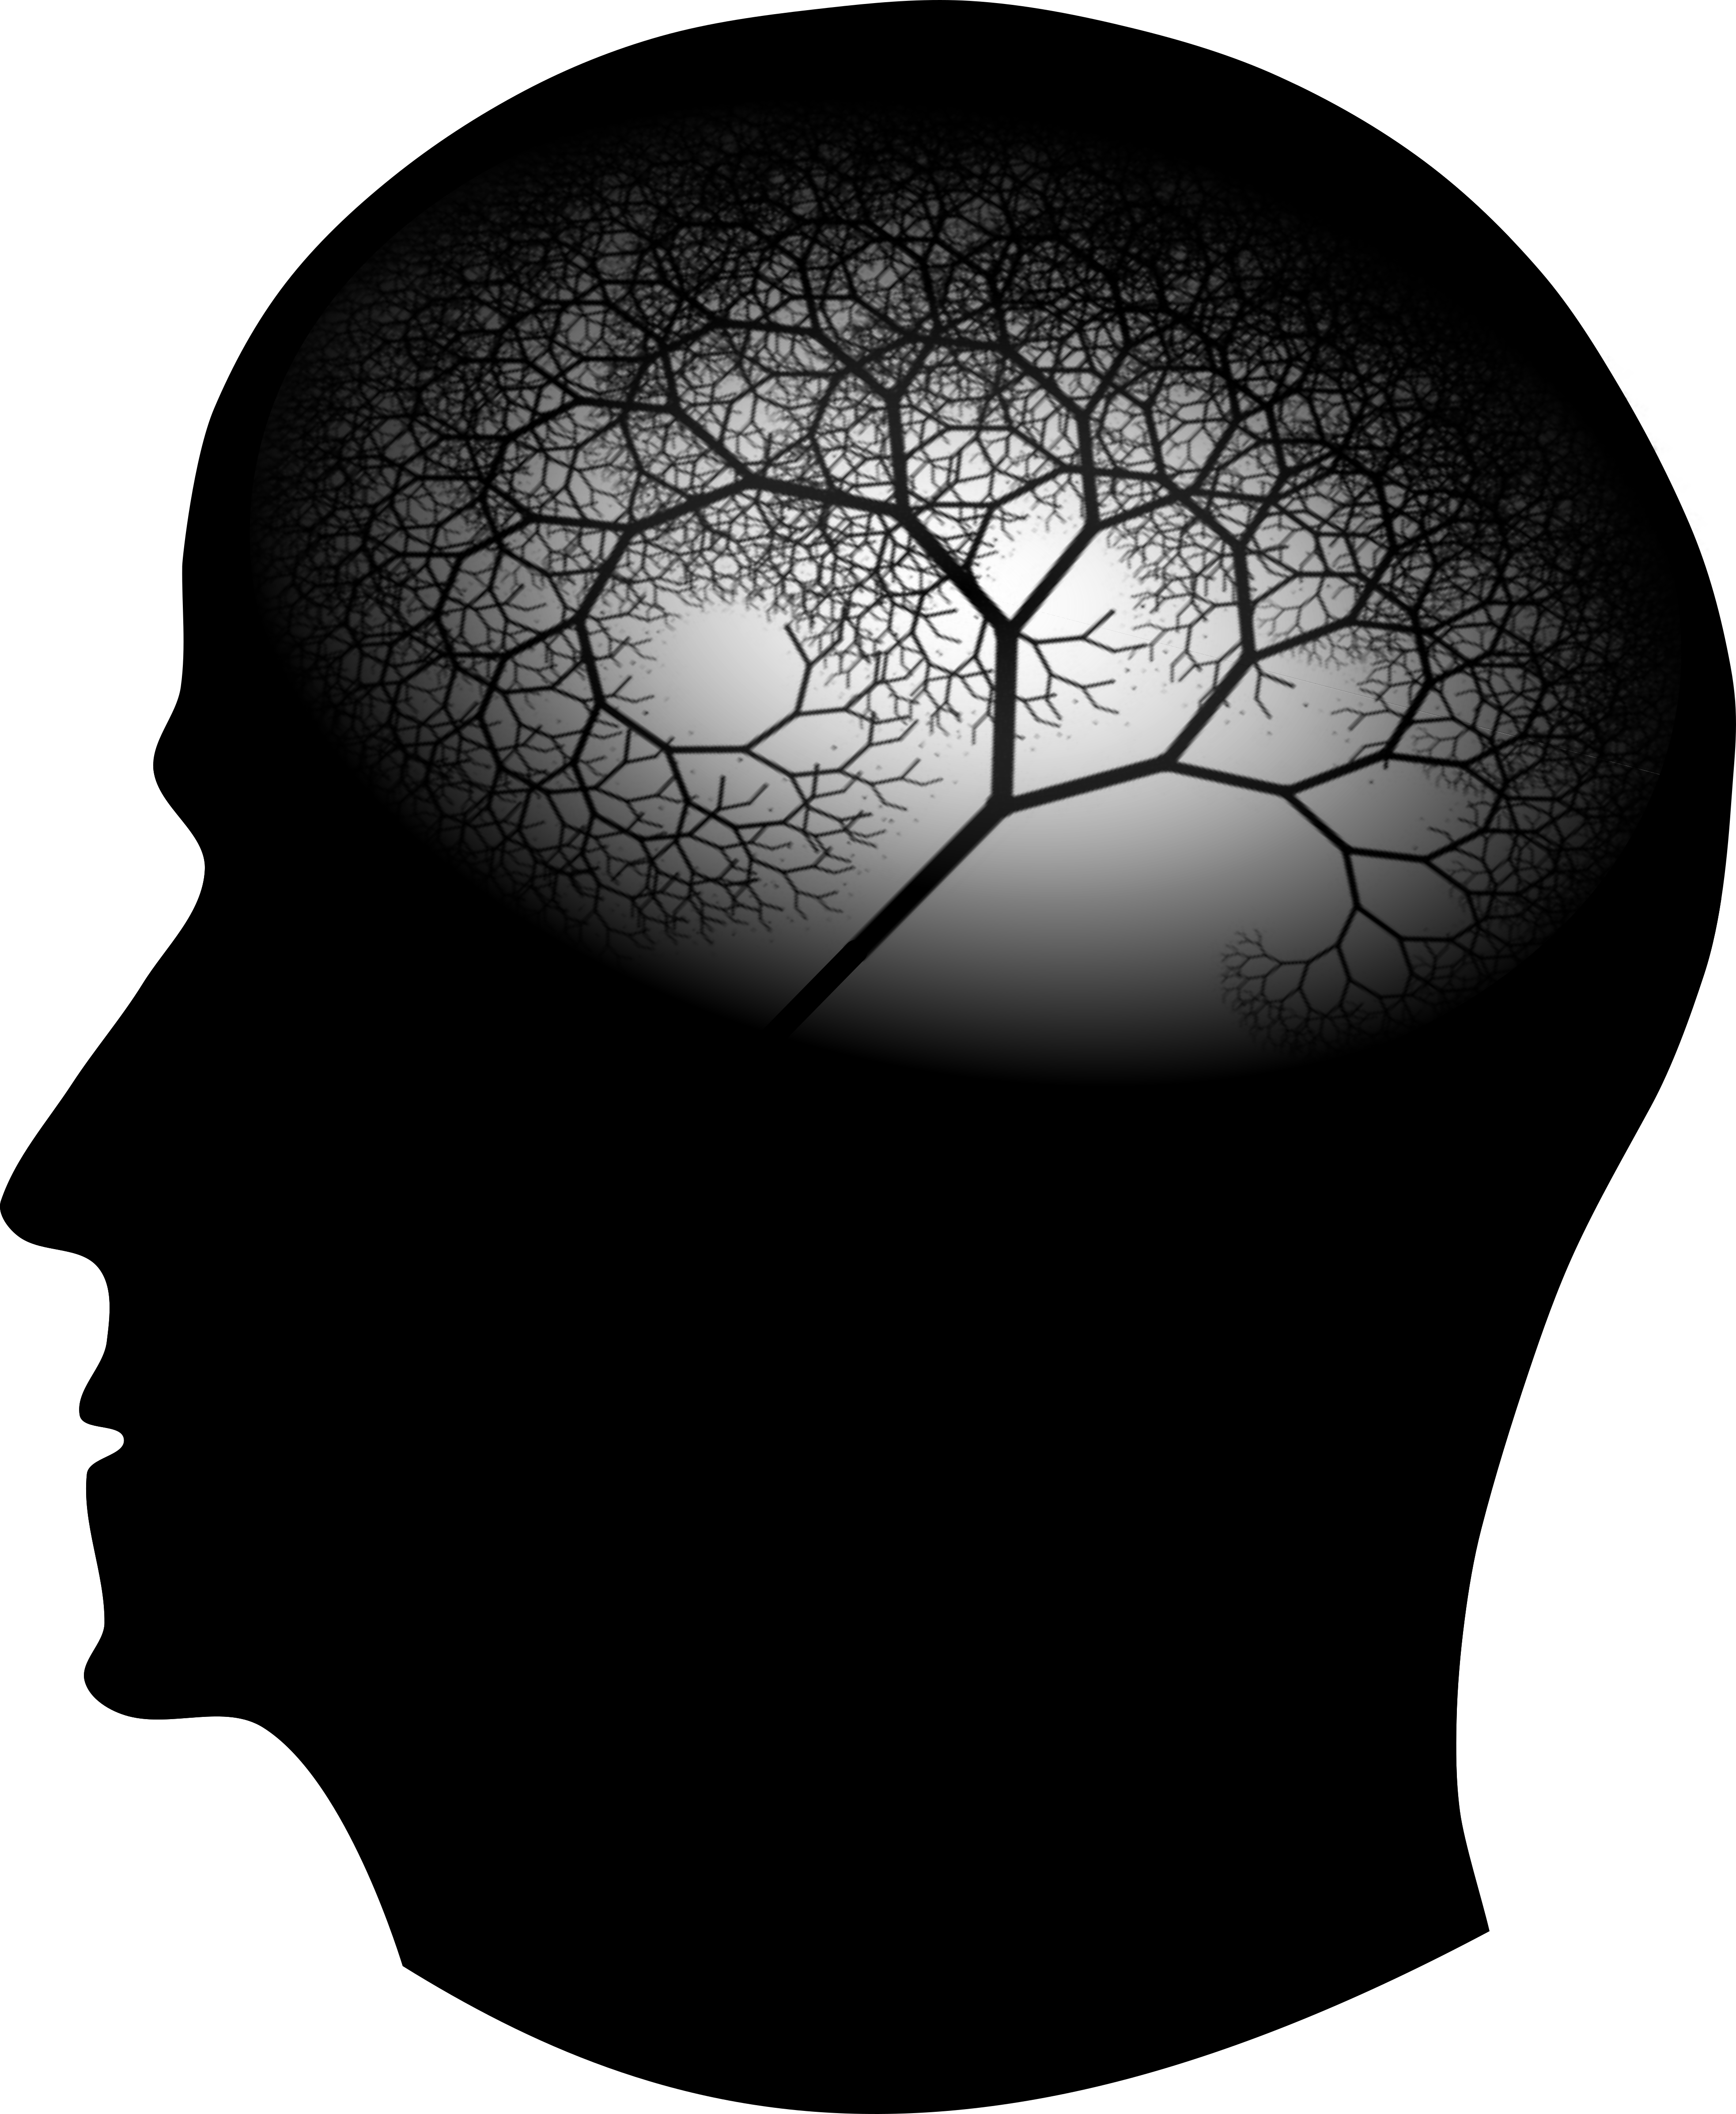
\includegraphics[width = 0.7\textwidth]{frase.png} 
\end{figure*}

\newpage

\setcounter{page}{1}
\pagenumbering{arabic}

%%%%%%%%%%%%%%%%%%%%%%%%%%%%%%%%%%%%%%%%%%%%%%%%%%%%%%%%%%%%%%%%%%%%%%%%%%%%%%%%%%%%%%%%%%%%%%%%%%%
%%%%%%%%%%%%%%%%%%%%%%%%%%%%%%%%%%%%%%%%%%%%%%%%%%%%%%%%%%%%%%%%%%%%%%%%%%%%%%%%%%%%%%%%%%%%%%%%%%%
%%%%%%%%%%%%%%%%%%%%%%%%%%%%%%%%%%%%%%%%%%%%%%%%%%%%%%%%%%%%%%%%%%%%%%%%%%%%%%%%%%%%%%%%%%%%%%%%%%%

\pagestyle{fancy}
%    \fancyhf{} 
    \fancyhead[LO]{\sectionmark}
    \fancyhead[RE]{\chaptermark}
    \fancyfoot[CE,CO]{}
    \fancyfoot[LE,RO]{\thepage}
    \renewcommand{\headrulewidth}{1.5pt}

%%%%%%%%%%%%%%%%%%%%%%%%%%%%%%%%%%%%%%%%%%%%%%%%%%%%%%%%%%%%%%%%%%%%%%%%%%%%%%%%%%%%%%%%%%%%%%%%%%%
%%%%%%%%%%%%%%%%%%%%%%%%%%%%%%%%%%%%%%%%%%%%%%%%%%%%%%%%%%%%%%%%%%%%%%%%%%%%%%%%%%%%%%%%%%%%%%%%%%%

\chapter*{Introducción}
\addcontentsline{toc}{chapter}{Introducción}

Gracias a los avances médicos del último siglo se ha incrementado la esperanza de vida y la calidad de vida. 
%
Desafortunadamente, también ha aumentado la presencia de enfermedades no-transmisibles asociadas con la edad. 
%
En México el sector de la población con más de 60 años de edad (considerados en alto riesgo para este tipo de enfermedades) contempló a 10 millones de personas en 2010, y en 2015 dicha cifra creció a 12 millones \cite{Censo10,Intercensal15}.
%
En este trabajo se destaca la demencia de entre las enfermedades asociadas con la edad.

La demencia consiste en el desarrollo de deficiencias cognoscitivas (especialmente en atención y memoria) suficientemente graves para interferir en las actividades del individuo.
%
Se considera que la demencia es irreversible, y no se han identificado curas definitivas \cite{PlanAlzheimer04}, debido a lo cual ha surgido un gran interés en definir y diagnosticar sus etapas tempranas.
%
El deterioro cognitivo leve (DCL), una etapa temprana de la demencia, se entiende como el desarrollo de deficiencias cognoscitivas \textit{objetivas} pero que no corresponden a daño físico del cerebro y no son lo suficientemente graves para calificarse como demencia.
%como ``una alteración adquirida y prolongada de una o varias funciones cognitivas, que no corresponde a un \textit{síndrome focal}\footnote{Se entiende por síndrome focal al daño en una estructura nerviosa específica, cuya causa es conocida (como una hemorragia o una embolia) y cuyo inicio sea inmediato y evidente. 
%%
%En contraparte, se considera que el inicio del DCL es \textit{insidioso} \cite{Petersen01}.
%} y que no cumple con criterios suficientes de gravedad para ser calificada como demencia" \cite{Robles02}.

%En el presente trabajo se delimita al DCL por fines de precisión, para lo cual se define el Posible Deterioro Cognitivo Leve (PDCL) como ``una disminución de las funciones cognitivas del sujeto con respecto las típicas de su edad y nivel de educación". 
%%
%En concreto, el desempeño de las funciones cognoscitivas para un individuo es medido usando la prueba neuropsicológica Neuropsi \cite{Ostrosky1999}; se considera un déficit si la puntuación obtenida es menor a un umbral predefinido para su grupo de edad y nivel de escolaridad. 
%%
%El umbral recomendado para la prueba Neuropsi debe calcularse como la media menos 3 desviaciones estándar de los puntajes típicos para individuos de cada grupo de edad y nivel de escolaridad. 
%%
%Estos parámetros fueron estimados para la población mexicana por Ostrosky-Solís y colaboradores \cite{Ostrosky1999}.

%El DCL puede detectarse por medio de diversos métodos que pueden ser complementarios. 
%%
%La forma más sencilla de detectarlo es por la autopercepción de fallas en la memoria o por la percepción de otros;
%es común que estos criterios subjetivos lleven a falsos negativos o falsos positivos, ésto por la percepción personal del nivel \textit{normal} de deterioro que se debe al envejecimiento.
%%
%Otras posibilidades para la detección incluyen la entrevista clínica de un especialista, o la aplicación de cuestionarios sobre dificultades en la memoria. 
%%
%Métodos más objetivos aún corresponden al diagnóstico con pruebas neuropsicológicas. 
%%
%Los análisis genéticos, químicos, de imágenes cerebral, entre otros, estudian el sistema nervioso central per se; dichas técnicas y otras, en combinación con las pruebas neuropsicológicas, permitirán diagnosticar más acertadamente el DCL y desentrañar los fenómenos neurobiológicos subyacentes.
%%Técnicas genéticas, químicas o de imágenes cerebrales u otras en elaboración, que pueden ser o no muy costosas, en su combinación con las neuropsicológicas, permitirían diagnosticar más acertadamente el DCL así como desentrañar sus correlatos neurobiológicos. 

Existen varios otros métodos alternativos para detectar --o definir-- el DCL; desde la autopercepción por parte del paciente, hasta análisis genéticos, químicos y de imagenología cerebral.
%
De entre estas técnicas se destaca a la polisomnografía (PSG), el registro conjunto de varias señales electrofisiológicas durante el sueño.
%
En particular, se considera una PSG compuesta por registros de electroencefalograma (EEG), electrooculograma (EOG) y electromiograma (EMG) para medir, respectivamente, actividad eléctrica cerebral, tono muscular y movimientos oculares.
%
El uso en particular de registros de PSG obedece principalmente a que (1) es una técnica relativamente barata y no invasiva, con relación al tipo de información que se obtiene, y (2) existe una cantidad moderadamente grande de marcadores para el DCL reportados usando la PSG.

Se ha encontrado, por ejemplo, correlaciones entre el DCL en adultos mayores con la \textit{presencia} de ciertos tipos de ondas cerebrales \cite{babiloni13,prichep94,prichep06}.
%
Sin embargo, otros estudios sugieren que el EEG durante el sueño es un mejor predictor del DCL [buscar y citar Baryet ??].
%
%El sueño MOR mejora la memoria y los procesos de atención mediante las entradas colinérgicas \cite{Braun} a través de pontine \cite{Datta2004} y las estructuras del basales del cerebro anterior \cite{Blake}. 
%%
%Durante el envejecimiento normal y especialmente durante el envejecimiento patológico, los procesos de atención y memoria se vuelven más vulnerables, y las neuronas colinérgicas son las más afectadas \cite{Schliebs11}. 
%
%El envejecimiento afecta a varias estructuras anatómicas que resultan en la pérdida de un eje dendrítico en las neuronas corticales que muestran una degradación en su complejidad fractal estructural \cite{Lipsitz}.

%%ANADÏ ESTO: y que normalmente estos marcadores electrofisiológicos se obtienen durante un estado de vigilia en reposo, es decir, despierto con ojos cerrados AGREGAR AQUÍ VARIAS REFS QUE ESTÁN AQUÍ ABAJITO  \cite{ Prichep et al., 1994; Rossini et al., 2006; Prichep et al., 2006; Rossini et al., 2008}. En general, se encontró que la potencia absoluta (PA) y relativa (PR) es mayor en la frecuencia de theta en estos pacientes y hay una correlación positiva con delta a más deterioro cognitivo en amplias regiones cerebrales y además la estabilidad de las fuentes de alfa en regiones posteriores sirve como un predictor confiable (Babiloni et al., 2013). Estos patrones se cree que representan alteraciones en el hipocampo relacionadas al deterioro cognitivo. 

%Montplaisir   citar aquí de la tesis de Gén la referencia, Julito, x fa hallan que el sueño MOR es mejor predictor que la vigilia

%arreglar la cita. Es decir, se espera hallar marcadores en la actividad eléctrica cerebral, muscular u ocular correlacionados con los déficits en alguna o varias funciones neuropsicológicas. Se usa el término de probable para ser congruentes con las especificaciones sobre los métodos, es decir, porque los análisis que se presentan pretenden arrojar mayores indicios anatómicos y fisiológicos sobre lo ya detectado con las pruebas.

En el presente trabajo se busca desarrollar métodos para determinar el DCL en base a registros de PSG en adultos mayores, como complemento a los resultados de pruebas neuropsicológicas.
%
Se mantiene presente que el deterioro cognitivo (más allá del DCL) no puede reducirse exclusivamente a tales mediciones; las conclusiones obtenidas usando registros de señales electrofisiológicas deben ser contrastadas siempre con resultados de análisis complementarios.


%El presente trabajo toma parte en el problema metodológico de que las señales electrofisiológicas típicamente representan procesos no--lineales y no--estacionarios, y sin 
%embargo suelen ser analizadas usando herramientas que suponen linealidad y estacionariedad. Se sabe que
%las señales biológicas son mayormente no estacionarias, pero en ventanas pequeñas de tiempo éstas son
%mayormente estacionarias.%AQUÍ PUEDEN PONER LA FIGURA DEL ARTÍCULO.
%Además estudios previos han demostrado que señales mayores de 20 segundos pueden ayudar 
%a inferir problemas neurológicos \cite{Cohen77}.
%
%En el caso particular del espectro de potencias, es común que sea calculado usando la 
%transformada de Fourier sobre segmentos cortos para evitar los \textit{efectos} de la 
%no--estacionariedad \cite{Kaiser00}.
%
%Es por ello que se buscan herramientas para verificar la estacionariedad débil (más detalles en 
%la sección de métodos)  en los registros electrofisiológicas, y con especial atención en la 
%posibilidad de que puedan usarse como marcadores de deterioro cognitivo.
%No se conocen otros estudios que empleen la prueba de Priestley-Subba-Rao (ref) que se explicará más adelante para probar estacionariedad con excepción de Rosales-Lagarde et al. (2017), sin embargo aquí se muestra con una mayor precisión.
%Rosales-Lagarde, A., Rodríguez-Torres, E.E., Enciso-Alva, J., Martínez-Alcalá, C., Vázquez-Tagle, G., Tetlamatzi-Montiel, M., Viveros, J. and López-Noguerola, J.S. (2017). Stationarity during REM sleep in Old Adults. Alzheimer´s and Dementia, P723-P724. doi: http://dx.doi.org/10.1016/j.jalz.2017.06.937

%%%%%%%%%%%%%%%%%%%%%%%%%%%%%%%%%%%%%%%%%%%%%%%%%%%%%%%%%%%%%%%%%%%%%%%%%%%%%%%%%%%%%%%%%%%%%%%%%%%
%%%%%%%%%%%%%%%%%%%%%%%%%%%%%%%%%%%%%%%%%%%%%%%%%%%%%%%%%%%%%%%%%%%%%%%%%%%%%%%%%%%%%%%%%%%%%%%%%%%

\section*{Antecedentes}
\addcontentsline{toc}{section}{Antecedentes}

En 2016 Vázquez-Tagle y colaboradores estudiaron el PDCL en adultos mayores del estado de Hidalgo con el método no lineal del Análisis de Fluctuaciones sin Tendencia (DFA, por sus siglas en inglés), encontrando efectivamente que los sujetos con PDCL presentan mayor ruido browniano en varias regiones en comparación con los pacientes sin PDCL\cite{VazquezTagle16}.
%
%Adicionalmente, la sugerencia de que sujetos con alteraciones neurológicas y deterioro cognitivo exhiben estacionariedad débil en sus 
%registros de EEG en mayor proporción (respecto a individuos sanos) fue sugerida anteriormente
%\cite{Cohen77}; aquél análisis se 
%refiere a su vez a trabajos anteriores sobre estacionariedad y normalidad en registros de EEG
%\cite{McEwen75,Sugimoto78,Kawabata73}.
%%
%Los estudios referidos se enmarcan en un primer intento de verificar que los registros 
%electrofisiológicos no pueden modelarse como señales \textit{simples} (lo contrario a señales 
%complejas).

%El presente trabajo tiene el objetivo de identificar concretamente
%los posibles cambios en los registros de PSG  debidos al PDCL. Siguiendo a Cohen \cite{Cohen77}, es posible predecir que en sujetos con PDCL habrá menores porcentajes de épocas estacionarias en comparación con sujetos controles, lo que puede deberse a una mayor cantidad de ondas lentas. Sin embargo, en esta tesis sólo se explorará si la primera condición se cumple, verificando el comportamiento estacionario de los registros.%CHECAR SI ASÍ ESTÁ BIEN DICHO...

%%%%%%%%%%%%%%%%%%%%%%%%%%%%%%%%%%%%%%%%%%%%%%%%%%%%%%%%%%%%%%%%%%%%%%%%%%%%%%%%%%%%%%%%%%%%%%%%%%%
%%%%%%%%%%%%%%%%%%%%%%%%%%%%%%%%%%%%%%%%%%%%%%%%%%%%%%%%%%%%%%%%%%%%%%%%%%%%%%%%%%%%%%%%%%%%%%%%%%%

En un estudio reciente, EEG de una noche polisomnografía de personas mayores con y sin deterioro cognitivo según las evaluaciones con el Neuropsi analizó el porcentaje de estacionariedad.  En sueño MOR el porcentaje fue menor que el del sueño NMOR y la vigilia, se obtuvo estacionariedad  como un índice para comparar NMOR versus sueño MOR en ambos grupos \cite{ROSALESLAGARDE2017}.

%El sueño MOR ha sido ampliamente reconocido como parte de la consolidación de la memoria, así como
%otras funciones cognitivas 
%\cite{Fishbein1971,Fishbein1977,Lucero1970,Pearlman1971,Pearlman1974,Smith1991}.
%%
%En el caso de adultos mayores, la correlación entre deterioro cognitivo y trastornos del sueño ha 
%sido reportada por varios autores a partir de estudios poblacionales 
%\cite{Amer13,Miyata13,Reid06,Potvin12}.
%%
%Tal correlación era de esperarse ya que los procesos de atención y memoria, por ejemplo, dependen de 
%los circuitos colinérgicos activados durante el sueño MOR \cite{Braun1997}; estos circuitos son 
%propensos a degradación estructural tanto en el envejecimiento normal como en el patológico,  y 
%especialmente en el segundo \cite{Schliebs11}.
%
%En 2016 Vázquez-Tagle y colaboradores estudiaron la epidemiología del DCL en adultos mayores dentro 
%del estado de Hidalgo y su posible relación con trastornos de sueño, encontrando efectivamente una 
%correlación entre una menor eficiencia del sueño (porcentaje de tiempo de sueño respecto al tiempo 
%en cama) y la presencia de deterioro cognitivo \cite{VazquezTagle16}.
%%
%En aquél estudio se efectuaron registros de PSG para algunos de los participantes, con la intención 
%de verificar que existen diferencias en los registros correspondientes a individuos con y sin DCL.
%%
%El presente trabajo se enmarca dentro de una reciente colaboración, con el objetivo de identificar concretamente
%los posibles cambios en los registros de PSG  ocurridos durante el DCL o PDC.
%
%La idea de que sujetos con deterioro cognitivo exhiban cambios en sus registros de PSG relacionados 
%a la estacionariedad débil, fue sugerida por Cohen en 1977 \cite{Cohen77}; aquél análisis se 
%refiere a su vez a trabajos anteriores sobre estacionariedad y normalidad en registros de EEG
%\cite{McEwen75,Sugimoto78,Kawabata73}.
%%
%Los estudios referidos se enmarcan en un primer intento de verificar que los registros 
%electrofisiológicos no pueden modelarse como señales \textit{simples} (lo contrario a señales 
%complejas).

%%%%%%%%%%%%%%%%%%%%%%%%%%%%%%%%%%%%%%%%%%%%%%%%%%%%%%%%%%%%%%%%%%%%%%%%%%%%%%%%%%%%%%%%%%%%%%%%%%%
%%%%%%%%%%%%%%%%%%%%%%%%%%%%%%%%%%%%%%%%%%%%%%%%%%%%%%%%%%%%%%%%%%%%%%%%%%%%%%%%%%%%%%%%%%%%%%%%%%%

\section*{Pregunta de investigación y objetivos}
\addcontentsline{toc}{section}{Pregunta de investigación y objetivos}

Los registros de PSG en adultos mayores, modelados como procesos estocásticos, ¿pueden considerarse como débilmente estacionarios?
%
¿Dicha caracterización es afectada si el individuo presenta PDCL?

%¿Las series de tiempo de los registros de polisomnografía en adultos mayores son débilmente estacionarias?
%%
%Si en efecto, son débilmente estacionarias ¿Ésta es distinta entre los sujetos con PDCL y sin PDCL?

%%%%%%%%%%%%%%%%%%%%%%%%%%%%%%%%%%%%%%%%%%%%%%%%%%%%%%%%%%%%%%%%%%%%%%%%%%%%%%%%%%%%%%%%%%%%%%%%%%%
%%%%%%%%%%%%%%%%%%%%%%%%%%%%%%%%%%%%%%%%%%%%%%%%%%%%%%%%%%%%%%%%%%%%%%%%%%%%%%%%%%%%%%%%%%%%%%%%%%%

%\subsection*{Hipótesis}
%
%Existen diferencias en la estacionariedad débil de la actividad eléctrica cerebral, muscular u ocular en adultos mayores con PDCL respecto a 
%individuos sanos. 
%\textit{presencia} deen registros de PSG.

%%%%%%%%%%%%%%%%%%%%%%%%%%%%%%%%%%%%%%%%%%%%%%%%%%%%%%%%%%%%%%%%%%%%%%%%%%%%%%%%%%%%%%%%%%%%%%%%%%%

\subsection*{Objetivo general}

Estudiar sobre pruebas estadísticas para detectar si una realización dada proviene de un proceso estocástico débilmente estacionario.
%
Usar tales pruebas sobre registros de PSG en adultos mayores con y sin PDCL.
%
Investigar si hay una relación entre la presencia de PDCL y la clasificación de los proceso estocásticos referidos como débilmente estacionarios.

% la presencia de más segmentos débilmente estacionarios se asocia con la condición de PDCL.

%%%%%%%%%%%%%%%%%%%%%%%%%%%%%%%%%%%%%%%%%%%%%%%%%%%%%%%%%%%%%%%%%%%%%%%%%%%%%%%%%%%%%%%%%%%%%%%%%%%

%\subsection*{Objetivos específicos}
%
%\begin{itemize}
%\item Estudiar la definición de estacionariedad para procesos estocásticos.
%
%\item Investigar cómo detectar, como prueba de hipótesis, si una serie de tiempo dada proviene
%de un proceso estocástico débilmente estacionario, y bajo qué supuestos 
%es válida dicha caracterización.
%
%\item Establecer si los registros de PSG durante las etapas de sueño son débilmente estacionarios.
%
%\item Investigar si la presencia de segmentos estacionarios en los registros es diferente si la
%PSG corresponde a un individuo con PDCL.
%\end{itemize}


\section*{Sobre la estructura del texto}
\addcontentsline{toc}{section}{Sobre la estructura del texto}

%En los capítulos del 1 al 3 se exponen tópicos que bien pueden considerarse como matemáticas puras: probabilidad, estimación de parámetros, pruebas de hipótesis, teoría de la medida, análisis funcional.

Debido al enfoque aplicado del presente trabajo, esta porción del texto fue estructurada pensando en dos tipos de lectores: por un lado aquellos interesados principalmente en los objetos matemáticos involucrados y sus conexiones, y por otro lado quienes ven los mismos como herramienta y esperan entenderlos mejor.
%
Los temas fueron ordenados pensando en el primer tipo de lector.
%
Para el segundo tipo de lector, se ha preparado en la figura \ref{intro:estructura} un \textit{mapa} del texto, pero principalmente de los temas sobre matemáticas.

En el primer capítulo se abordan varios temas preliminares sin lujo de detalles, con la finalidad de presentar un texto autocontenido;
%
la finalidad del capítulo es definir formalmente los procesos estocásticos, espacios de Hilbert y estimadores.

%El presente trabajo está conformado por 6 capítulos y un apéndice. El primer capítulo aborda conceptos preliminares como medida, integración, variables aleatorias, estimadores, pruebas de hipótesis, proceso estocásticos, espacios de Hilbert y la transformada de Fourier.

%El objeto principal de este trabajo es el estudio de la estacionariedad débil en registros de polisomnograma de adultos mayores para investigar si es posible usarlos para

En el segundo capítulo se definen los procesos estocásticos débilmente estacionarios, al conjunto de éstos se les da estructura de espacio de Hilbert, y finalmente se usa dicha estructura para definir el espectro de potencias como una generalización de la transformada de Fourier.
%
Una porción importante del capítulo trata sobre la estimación efectiva del espectro de potencias a partir de observaciones dadas de un proceso estocástico.

%En el segundo capítulo se expone una serie de temas relacionados con la \textit{estadística en el dominio espectral}, es decir, obtener el espectro de potencias de un proceso estocástico --particularmente de procesos débilmente estacionarios.
%%
%Debido a la notoria relación mutua entre estos temas, se decidió ilustrar en la figura \ref{intro:estructura} la red de temas según dependen unos de otros.

En el tercer capítulo se define el \textit{espectro evolutivo}, una generalización del espectro de potencias para una familia de procesos que no son débilmente estacionarios.
%
%En cierto sentido, el espectro evolutivo se define de modo que induzca una estructura parecida a la descrita en el capítulo dos, incluyendo la forma en que puede ser estimado.
%
Al final se expone una aplicación aparente menor del espectro evolutivo, pero que es fundamental para el resto del presente trabajo: la prueba de Priestley Subba-Rao. 
%
Esta prueba verifica --como prueba de hipótesis-- si el espectro evolutivo de un proceso puede reducirse a un espectro de potencias; en otras palabras, si un proceso es débilmente estacionario.

%En el tercer capítulo se expone el \textit{espectro evolutivo}, una generalización del espectro de potencias para procesos no estacionarios.
%%
%Como el espectro evolutivo de un proceso débilmente estacionario se reduce al espectro de potencias, se describe una metodología para detectar estacionariedad débil.

%
%Naturalmente, esta tarea implica la exposición de varios otros temas relativos a las condiciones bajo las cuales el espectro de potencias está bien definido, así como las condiciones bajo las cuales es posible su estimación.

%El objetivo final del capítulo es presentar una prueba de estacionariedad débil y que es usada para estudiar las propiedades de los registros.

En el cuarto capítulo se presentan conceptos de índole \textit{fisiológica}: psicología, psicometría, electroficiología.
%
El objetivo del capítulo es describir el DCL y cómo se detecta, describir qué es el sueño y como se analiza (en este caso a partir de la polisomnografía), y mencionar la relación entre el sueño y el DCL.

%En el cuarto capítulo se presentan conceptos preliminares de índole fisiológica como detección de deterioro cognitivo y su relación con el sueño. En particular se explora el estudio del sueño a través de la polisomnografía.

En el capítulo quinto se describe cómo se utilizó la prueba de estacionariedad débil para estudiar los registros de polisomnografía.
%
En el capítulo sexto se discuten los resultados obtenidos, y se concluye que la técnica utilizada no es un marcador diagnóstico para el DCL; se reportan algunos hallazgos incidentales.


%
%
%En el capítulo quinto describe cómo se aplica la metodología descrita en los capítulos anteriores.
%%
%Los registros son divididos en segmentos, llamados \textit{épocas}, que son analizadas en tres niveles:
%\begin{itemize}
%\item Se prueba la homogeneidad de cada época
%\item Se estudian las características de las distintas épocas dentro 
%\end{itemize}
%
%En el capítulo sexto se discuten los resultados obtenidos y se exponen las conclusiones.

%En el capítulo 2 se describe lo  que es el deterioro cognitivo leve y cómo se detecta a nivel de comportamiento, así como se describen varios esfuerzos por detectar este padecimiento en base a mediciones más objetivas a nivel de sistema (en particular, con el enfoque de mediciones de la actividad cerebral). 
%
%Dado que se ha reportado relaciones entre el sueño MOR y la memoria a corto y largo plazo, se dedica una sección a describir el sueño y sus características, y su estudio a través de la polisomnografía.
%
%En el capítulo 3 se muestran los sujetos de estudio; debido a que el trabajo se enmarca en una colaboración, se describe la metodología usada en trabajos anteriores usando esta misma base datos, y se considera como conocidos los datos sobre pruebas neuropsicológicas y los registros de PSG se consideran conocidos. 
%%
%Posteriormente se expone la metodología original en este trabajo correspondiente en cuanto el uso que se da a la prueba de PSR. El análisis se efectúa en dos niveles: 
%\begin{itemize}
%\item Para cada sujeto, los registros son segmentados en una colección de ventanas (épocas) que se clasifican como etapas según sus características tipificadas\footnote{Estas características son en su mayoría visuales, y se encuentran reguladas por lineamientos internacionales como aquél de la AASM \cite{AASM07}} , debido a la heterogeneidad del sueño, tiene sentido tratar a estas épocas como una población
%\item A nivel de grupo, algunas características son comparadas entre sujetos
%\end{itemize}
%conviene destacar que la heterogeneidad en los registros puede observarse intuitivamente de manera gráfica.

\begin{figure}
\centering
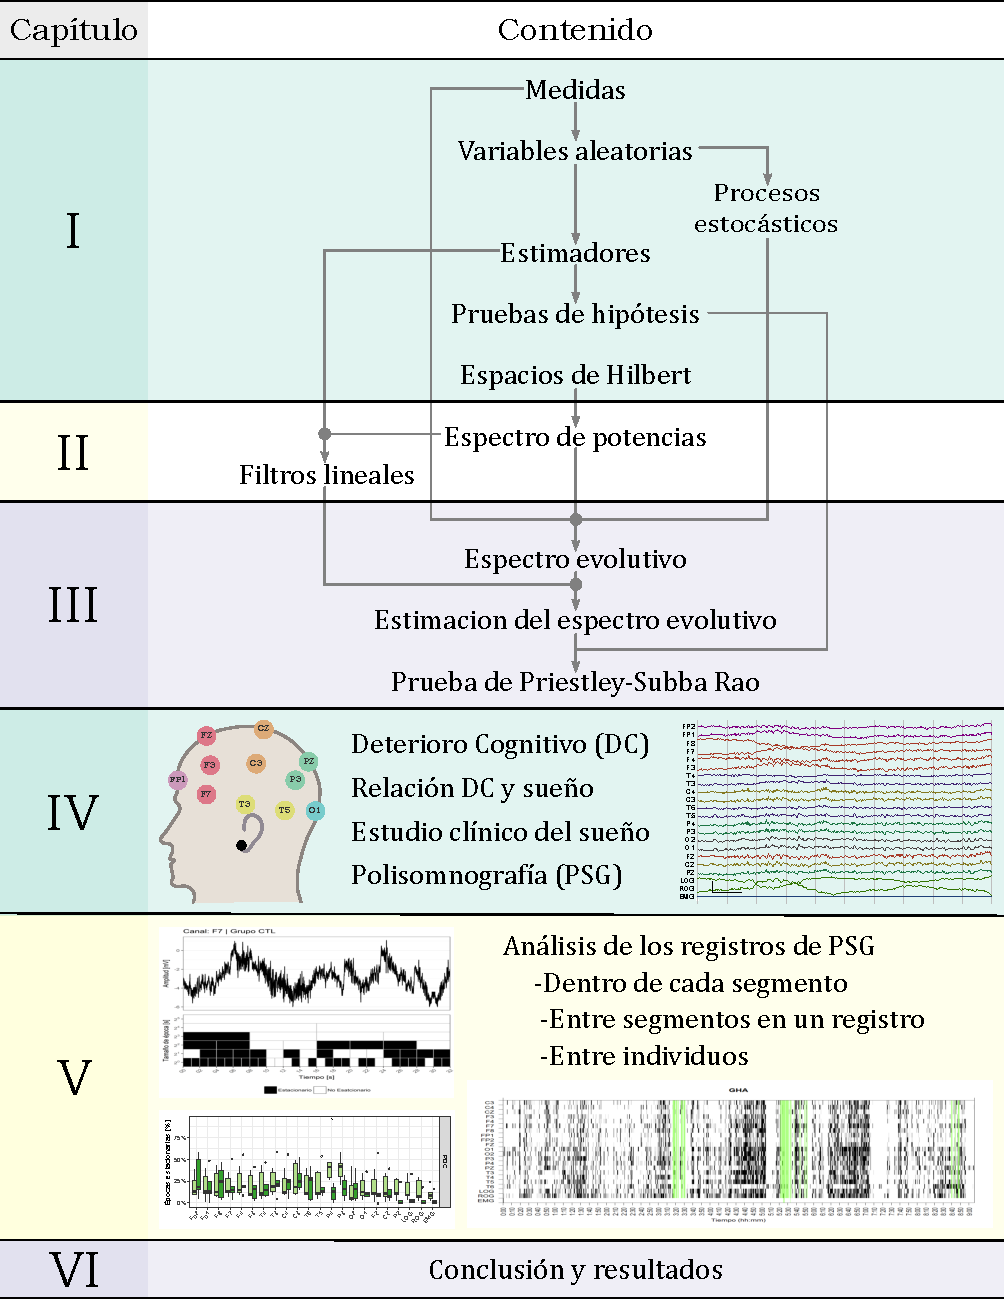
\includegraphics[width=.9\textwidth]{./estructura_texto_v2.pdf}
\caption[Estructura de la tesis]{Se ilustra gráficamente las \textit{dependencias} respecto a los tópicos de matemáticas, es decir, los temas que deben discutirse antes que otros. El resto del texto (incluyendo los tópicos de fisiología) son expuesto de forma más \textit{secuencial}, por lo que no se consideró necesario ilustrar sus dependencias.}
\label{intro:estructura}
\end{figure}

%%%%%%%%%%%%%%%%%%%%%%%%%%%%%%%%%%%%%%%%%%%%%%%%%%%%%%%%%%%%%%%%%%%%%%%%%%%%%%%%%%%%%%%%%%%%%%%%%%%
%%%%%%%%%%%%%%%%%%%%%%%%%%%%%%%%%%%%%%%%%%%%%%%%%%%%%%%%%%%%%%%%%%%%%%%%%%%%%%%%%%%%%%%%%%%%%%%%%%%

%%%%%%%%%%%%%%%%%%%%%%%%%%%%%%%%%%%%%%%%%%%%%%%%%%%%%%%%%%%%%%%%%%%%%%%%%%%%%%%%%%%%%%%%%%%%%%%%%%%
%%%%%%%%%%%%%%%%%%%%%%%%%%%%%%%%%%%%%%%%%%%%%%%%%%%%%%%%%%%%%%%%%%%%%%%%%%%%%%%%%%%%%%%%%%%%%%%%%%%
%%%%%%%%%%%%%%%%%%%%%%%%%%%%%%%%%%%%%%%%%%%%%%%%%%%%%%%%%%%%%%%%%%%%%%%%%%%%%%%%%%%%%%%%%%%%%%%%%%%

\chapter{Preliminares}

El lector interesado puede revisar mayores detalles sobre teoría de la medida, probabilidad y estadística en los libros \textit{``Probability for Statisticians"} por Galen R. Shorack \cite{probabilidad_shorack} y \textit{``Statistical Theory"} por Bernard W. Lindgren \cite{estadistica_lindgren}.
Redactar también \cite{estacionariedad_lindgren}.

%%%%%%%%%%%%%%%%%%%%%%%%%%%%%%%%%%%%%%%%%%%%%%%%%%%%%%%%%%%%%%%%%%%%%%%%%%%%%%%%%%%%%%%%%%%%%%%%%%%

\section{Medidas}

\begin{definicion}%[$\boldsymbol{\sigma}$-álgebra]
Sea $\Omega$ un conjunto y sea $\mathcal{U}$ una familia de subconjuntos de $\Omega$. Se dice que 
$\mathcal{U}$ es una \textbf{$\boldsymbol{\sigma}$-álgebra} si cumple
\begin{itemize}
\item $\Omega \in \mathcal{U}$
\item $A \in \mathcal{U} \Rightarrow A^{C} \in \mathcal{U}$
\item 
$ \displaystyle \{ A_n \}_{n\in \mathbb{N}} \subseteq \mathcal{U} 
\Rightarrow \cup_{n\in \mathbb{N}} A_n \in \mathcal{U}$
\end{itemize}
Donde $A^{C}$ es el complemento de $A$ en $U$
\end{definicion}

Los elementos de una $\sigma$-álgebra se denominan \textbf{conjuntos medibles}. 

\begin{definicion}
Sea $\Omega$ un conjunto y $\mathcal{A} \subseteq \Omega$ una familia de subconjuntos. Se define a $\sigma(\mathcal{A})$, la $\sigma$-álgebra generada por $\mathcal{A}$, como la intersección de todas las $\sigma$-álgebras que contienen a $\mathcal{A}$  
\end{definicion}

En el contexto de la probabilidad, es particularmente importante la $\sigma$-álgebra de Borel, definida como
\begin{equation}
\mathcal{B} = \sigma\left( \left\{ \left( -\infty , a \right] \subset \R \lvert a\in \R \right\} \right)
\end{equation}
Este tipo de $\sigma$-álgebras puede definirse sencillamente para algún subconjunto $A \subset \R$
\begin{equation}
\mathcal{B}_A = \sigma\left( \left\{ \left( -\infty , a \right] \cap A \subset \R \lvert a\in \R \right\} \right)
\end{equation}

\begin{definicion}
Sea $\Omega$ un conjunto y $\mathcal{U}$ una $\sigma$-álgebra definida en $\Omega$. El par $(\Omega,\mathcal{U})$ será referido como \textbf{espacio de medida}. Por nomenclatura, $\Omega$ es referido como \textit{espacio muestral} y $\mathcal{U}$ como \textit{$\sigma$-álgebra de sucesos}.
\end{definicion}

\begin{definicion}%[Medida]
Sea $(\Omega, \mathcal{U})$ un espacio de medida. Se dice que una función $\mu : \mathcal{U} \rightarrow \R_+$ es una \textbf{medida} si cumple que
\begin{itemize}
\item $\mu(\emptyset) = 0$
\item Si $\{ A_n \}_{n\in \mathbb{N}} \subseteq \mathcal{U}$ son tales que 
$A_n \cap A_m = \emptyset \Leftrightarrow m\neq n$, entonces
$$ \mu\left( \bigcup_{n\in \mathbb{N}} A_n \right) = \sum_{n\in \mathbb{N}} \mu(A_n)$$
\end{itemize}
Donde $\R_+ = \{ x\in \R | 0 \leq x \} \cup \{ \infty \}$ y $\emptyset$ es el conjunto vacío.
La terna $(\Omega,\mathcal{U},\mu)$ será referida como \textbf{espacio de medida}.
\label{medida}
\end{definicion}

\begin{definicion}%[Medida $\boldsymbol{\sigma}$-finita]
Sea $(\Omega,\mathcal{U},\mu)$ un espacio de medida. Se dice que $\mu$ es 
\textbf{$\boldsymbol{\sigma}$-finita} si existen una familia de conjuntos medibles $\{ A_n \}_{n\in \mathbb{N}}$ tales que
\begin{itemize}
\item $\mu\left( A_n \right) < \infty$
\item $ \bigcup_{n\in \mathbb{N}} A_n = \Omega$
\end{itemize}
\end{definicion}

\begin{definicion}
Considérese el espacio medible $(\R, \mathcal{B})$, con $\mathcal{B}$ la $\sigma$-álgebra de Borel. Se define la medida de Lebesgue, $\mu_L$, la medida en el espacio mencionado tal que 
\begin{equation}
\mu_L([a,b]) = b-a
\end{equation}
para cualesquiera $a,b \in \R$ con $a<b$
\end{definicion}

%\begin{proposicion}
%Sea $(\Omega,\mathcal{U},P)$ un espacio de probabilidad. Sea $\{ A_n \}_{n\in \mathbb{N}}$ una amilia de conjuntos medibles tales que 
%\begin{itemize}
%\item $A_n \subset A_{n+1}$ para todo $n \in \N$
%\item Existe un conjunto medible $A$ tal que $\cup_{n\in \N} A_n = A$
%\end{itemize}
%Entonces
%\begin{equation}
%\lim_{n\rightarrow \infty} P(A_n) = P(A)
%\end{equation}
%\end{proposicion}
%\begin{proof}
%Nótese que
%\begin{align*}
%P(A) &= P\left( \cup_{n\in \N} A_n \right) \\
%\end{align*}
%\end{proof}

\subsection{Integración en espacios medibles}

\begin{definicion}
Sea $(\Omega, \mathcal{U}, \mu)$ un espacio de medida y sea $f:\omega \rightarrow \R_+$ una función medible no-negativa. Sea $A\in \mathcal{U}$ un conjunto arbitrario y $\mathcal{C}_A \subset \mathcal{U}$ el conjunto de las particiones de $A$ en una cantidad finita de conjuntos medibles.
Se define la \textbf{integral de $f$ respecto a $\mu$ en el conjunto $A$} como
\begin{equation}
\int_A f(x) \mu(x) := \sup_{\mathcal{C}_A} \left[ \sum_{j=1}^{n} f(\lambda) \mu(E_m) \right]
\end{equation}
Donde $\mathcal{C}_A = \{ E_1, E_2, \dots, E_n \}$
\end{definicion}

\begin{definicion}
Sea $(\Omega, \mathcal{U}, \mu)$ un espacio de medida y sea $f:\omega \rightarrow \R_+$ una función medible. Se definen las funciones $f^{+}$ y $f^{-}$ como
\begin{align*}
f^{+}(x) &= \max (f(x), 0 ) \\
f^{-}(x) &= -\min (f(x), 0 )
\end{align*}
Se dice que $f$ es integrable en $A$ respecto a $\mu$ si cumple que $\int_A f^{+}(\lambda) d\mu(\lambda) < \infty$ y $\int_A f^{-}(\lambda) d\mu(\lambda) < \infty$; si así fuere, se define
\begin{equation}
\int_A f(\lambda) d\mu(\lambda) := \int_A f^{+}(\lambda) d\mu(\lambda) - \int_A f^{-}(\lambda) d\mu(\lambda)
\end{equation}
\end{definicion}

\begin{proposicion}
Sean $(\Omega_1,\mathcal{U}_1)$ y $(\Omega_2,\mathcal{U}_2)$ espacios medibles y $\mu$ una medida sobre el primero. Una función $g$ es integrable en $A \in \mathcal{U}_2$ respecto a $\mu_f$ si y sólo si $g \circ f$ es integrable en $f^{-1}(A)$ respecto a $\mu$. En dado caso, se satisface que
\begin{equation}
\int_A g(\lambda) d\mu_f(\lambda) = \int_{f^{-1}(A)} g \circ f (\lambda) d\mu(\lambda)
\end{equation}
\end{proposicion}
%\begin{proof}
%asdasd [?] pagina 47 del manual
%\end{proof}

%\begin{proposicion}
%Sea $(\Omega, \mathcal{U}, \mu)$ un espacio de medida y sea $f:\omega \rightarrow \R_+$ una función medible no-negativa. La función $\mu_f$ definida como
%\begin{equation}
%\mu_f(A) := \int_A f(\lambda) \mu(\lambda)
%\end{equation}
%es una medida en el espacio medible $(\Omega, \mathcal{U})$
%\end{proposicion}
%
%\begin{proof}
%[?] Si se necesita, en la pagina 39 el manual
%\end{proof}

%\begin{proposicion}
%Sean $f$ y $g$ funciones integrables en $A$ con respecto a $\mu$ y sean $\alpha, \beta \in \R$ arbitrarios. Se cumple que la función $(\alpha f + \beta g)$ es integrable y
%\begin{equation}
%\int_A \left[ \alpha f + \beta g \right] (\lambda) \mu(\lambda) = \alpha \int_A f(\lambda) \mu(\lambda) + \beta \int_A 
%\end{equation}
%\end{proposicion}

%%%%%%%%%%%%%%%%%%%%%%%%%%%%%%%%%%%%%%%%%%%%%%%%%%%%%%%%%%%%%%%%%%%%%%%%%%%%%%%%%%%%%%%%%%%%%%%%%%%

\section{Variables aleatorias}

Si una medida $\mu$ es acotada en todo el espacio de eventos se dice que es una \textbf{medida finita} (no confundir con $\sigma$-finita). 
%
Una medida de probabilidad puede entenderse como un caso particular de medida finita sobre los reales.

\begin{definicion}
El espacio de medida $(\Omega,\mathcal{U},P)$ se dice un \textbf{espacio de probabilidad} si satisface que $P(\Omega) = 1$ 
\end{definicion}

\begin{definicion}
Sean $(\Omega_1,\mathcal{U}_1)$ y $(\Omega_2,\mathcal{U}_2)$ dos espacios medibles. Se dice que una función $f: \omega_1 \rightarrow \Omega_2$ es \textbf{medible} si para todo $A\in \mathcal{U}_2$
$f^{-1}(A)\in\mathcal{U}$
\end{definicion}

\begin{definicion}
Sea $(\Omega,\mathcal{U})$ un espacio medible y $(I,\mathcal{B}_I,P)$ un espacio de probabilidad. Una \textbf{variable aleatoria} es una función medible $X: \Omega \rightarrow \mathcal{B}_I$ entre estos espacios
\end{definicion}

Siendo $X$ una variable aleatoria, intuitivamente se puede definir la función de densidad de probabilidad de un conjunto medible $A \in \mathcal{B}$ como
\begin{equation}
P_X(A) = P\left( X^{-1} \left( A \right) \right)
\end{equation}

%Los espacios de probabilidad pueden definirse para una gran variedad de conjuntos; por simplicidad, en el presente texto únicamente se manejan espacios de probabilidad de la forma $(I,\mathcal{B}_I,P)$, con $I\subseteq \R$ un intervalo.

%Comunmente se asocia el resultado de un experimento \textit{aleatorio} con un espacio de probabilidad; el espacio muestral correspondería a los resultados posibles, y la medida representaría la \textit{probabilidad} de que el resultado ocurra en determinado conjunto.
%%
%Es común interpretar que si la probabilidad de un conjunto medible es $p$, entonces se espera que el resultado ocurra en dicho conjunto el $100*p \%$ de las ocasiones que se repita el experimento.

\begin{definicion}%[Función de Probabilidad Acumulada]
Sea $(\R,\mathcal{B},P)$ un espacio de probabilidad. La \textbf{función de probabilidad acumulada}, $F : \R \rightarrow [0,1]$, se define como
\begin{equation*}
F (x) := P\left( \left(-\infty,x \right] \right)
\end{equation*}
\end{definicion}

Por comodidad, se define una notación alterna para la función de probabilidad acumulada de $X$ como
\begin{equation}
P_X(x\leq x) := F_X(x) = P_X\left( \left( -\infty,x \right] \right)
\end{equation}
Si se puede definir una función de densidad de probabilidad para $X$, entonces puede escribirse
\begin{equation}
P(x\in A) = \int_A f_X(\lambda) d\lambda 
\end{equation}

Una función de probabilidad acumulada satisface las siguientes propiedades
\begin{itemize}
\item Para cualesquiera $x,y\in \R$, $x < y \Rightarrow F(x) < F(y)$
\item Pra cualquier $x\in\R$, $F(x) = \lim_{x\rightarrow x^{-}} F(x) + P(\{x\})$
\item $\lim_{x\rightarrow +\infty} F(x) = 1$
\item $\lim_{x\rightarrow -\infty} F(x) = 0$
\end{itemize}

Conviene considerar las funciones que satisface las condiciones anteriores, referidas simplemente como \textbf{función de distribución}, pero que no necesariamente provienen de un espacio de probabilidad. Naturalmente, una función de distribución $F$ puede inducir una medida $\mu$.

\begin{proposicion}
Sea $F:\R \rightarrow \R$ una función de distribución; se puede contruir una medida $\mu_F$ sobre el espacio medible $(\R, \mathcal{B})$ tal que la función de probabilidad acumulada asociada al espacio de probabilidad $(\R, \mathcal{B}, \mu_F)$ es exactamente $F$.
%
La medida $\mu_F$ será referida como la \textbf{medida inducida} por $F$.
\end{proposicion}
%\begin{proof}
%Para cualesquiera $a, b \in \R$, puede escribirse
%\begin{equation}
%\mu((a,b]) := F(b) - F(a)
%\end{equation}
%[? pag 18, 25 del libro de teorei ade la medida],
%se necesita teorema de extension de caratheodory
%\end{proof}

Así entonces, es perfectamente posible definir variables aleatorias especificando su respectiva función de probabilidad acumulada.

%\begin{definicion}
Cuando dos variableas aleatorias $X, Y$ tienen la misma función de densidad de probabilidad, se denota como
\begin{equation}
X \sim Y
\end{equation}
%\end{definicion}

\begin{ejemplo}
Si una variable aleatoria tiene una función de distribución de probabilidad de la forma
\begin{equation}
F(x) = \begin{cases}
0 &, x < 0 \\
p &, 0 \leq x < 1 \\
1 &, 1 \leq x
\end{cases}
\end{equation}
para algún $p \in [0,1]$. Se dice entonces que $X$ sigue una \textbf{distribución de Bernaulli} con parámetro $p$, y se denota por $X\sim \text{B}(p)$.
\end{ejemplo}

\begin{ejemplo}
Si una variable aleatoria tiene una función de distribución de probabilidad de la forma
\begin{equation}
F(x) = \begin{cases}
0 &, x < 0 \\
1 &, z \leq x
\end{cases}
\end{equation}
para algún $p \in \R$. Se dice entonces que $X$ sigue una \textbf{distribución degenerada} con parámetro $k$, y se denota por $X\sim \text{D}(p)$.
\end{ejemplo}

\begin{ejemplo}
Si una variable aleatoria tiene una función de distribución de probabilidad de la forma
\begin{equation}
F(x) = \frac{1}{\sqrt{2 \pi \sigma^{2}}} \int_{-\infty}^{x} e^{-\frac{(x-\mu)^{2}}{2}} dx
\end{equation}
para algunos $\mu, \sigma \in \R$. Se dice entonces que $X$ sigue una \textbf{distribución normal} con parámetros $\mu$ y $\sigma^{2}$, y se denota por $X\sim \text{N}(\mu,\sigma^{2})$.
\end{ejemplo}

%%%%%%%%%%%%%%%%%%%%%%%%%%%%%%%%%%%%%%%%%%%%%%%%%%%%%%%%%%%%%%%%%%%%%%%%%%%%%%%%%%%%%%%%%%%%%%%%%%%

\subsection{Convergencia de variables aleatorias}

\begin{definicion}
Sea $\{ F_n \}_{n\in \N}$ una sucesión de funciones de probabilidad acumulada, correspondientes a la sucesión de varaibles aleatorias reales $\{ X_n \}_{n\in \N}$. Se dice que la sucesión $\{ X_n \}_{n\in \N}$ \textbf{converge en distribución} a una variable aleatoria $X$ si, para todo $x\in \R$, se cumple que
\begin{equation}
\lim_{n\rightarrow\infty} F_n(x) = F(x)
\end{equation}
donde $F$ es la función de probabilidad acumulada de $X$.
\end{definicion}

\begin{definicion}
Sea $\{ F_n \}_{n\in \N}$ una sucesión de funciones de probabilidad acumulada, correspondientes a la sucesión de varaibles aleatorias reales $\{ X_n \}_{n\in \N}$. Se dice que la sucesión $\{ X_n \}_{n\in \N}$ \textbf{converge en probabilidad} a una variable aleatoria $X$ si, para todo $x\in \R$, se cumple que
\begin{equation}
\lim_{n\rightarrow\infty} P\left( \abso{X_n-X} < \varepsilon \right) = 1
\end{equation}
donde, para cada $n$, $P$ es la medida de probabilidad para el vector $[X_n, X]$.
\end{definicion}

%%%%%%%%%%%%%%%%%%%%%%%%%%%%%%%%%%%%%%%%%%%%%%%%%%%%%%%%%%%%%%%%%%%%%%%%%%%%%%%%%%%%%%%%%%%%%%%%%%%

\subsection{Variables aleatorias continuas y discretas}

\begin{definicion}
Una función $F: \R \rightarrow \R$ se dice \textbf{absolutamente continua} si para cualquier $\varepsilon>0$ arbitrario existe un $\delta>0$ y una familia de intervalos, $\{ [a_n, b_n]\}_{n\in \N}$, tal que
\begin{equation}
\sum_{n\in \N} \abso{b_n - a_n} < \delta 
\end{equation}
\begin{equation}
\sum_{n\in \N} \abso{F(b_n) - F(a_n)} < \varepsilon 
\end{equation}
\end{definicion}

Se dice que una medida de probabilidad $P$ es \textbf{continua} si su función de probabilidad acumulada es absolutamente continua.

%\begin{proposicion}
Si una medida de probabilidad $F$ es absolutamente continua, entonces existe una función $f$ tal que 
\begin{equation}
F(x) = \int_{-\infty}^{x}f(y) dy
\end{equation}
Se dice que $f$ es la \textbf{función de densidad de probabilidad}.
%\end{proposicion}

Sea $P$ una medida de probabilidad, se define su \textbf{soporte} como
\begin{equation}
\mathcal{D}_P = \left\{ x\in \R \lvert P\left( \left\{ x\right\} \right)>0 \right\}
\end{equation}
%
Se dice que una medida de probabilidad, $P$, es \textbf{discreta} si su soporte es numerable.

%\begin{proposicion}
Si una medida de probabilidad $F$ es discreta, entonces existe una finito o infinito numerable $Q_F=\{q_n\}_{n\in \N}$ tal que 
\begin{equation}
F(x) = \sum_{n\leq x} q_n F({q_n})
\end{equation}
Es posible construir una función de densidad de probabilidad para $F$ como
\begin{equation}
f(x) = \begin{cases}
F({x}) &, x\in Q_F \\
0 &, \text{otro caso}
\end{cases}
\end{equation}
%\end{proposicion}

Naturalmente es posible construir medidas de probabilidad que no sean ni continuas ni discretas. Por ejemplo, considérese la función de Cantor $K$ que puede ser definida iterativamente como
\begin{equation}
K_{n+1}(x) =
\begin{cases}
\frac{1}{2} K_n(3 x) &, 0\leq x \leq \frac{1}{3} \\
\frac{1}{2} K_n(3 x-2) + \frac{1}{2} &, 0\leq x \leq \frac{1}{3} \\
0 &, \text{otro caso}
\end{cases}
\end{equation}
con $K_0(x) = x$ y $K := \lim_{n\rightarrow \infty} K_n$

\begin{figure}
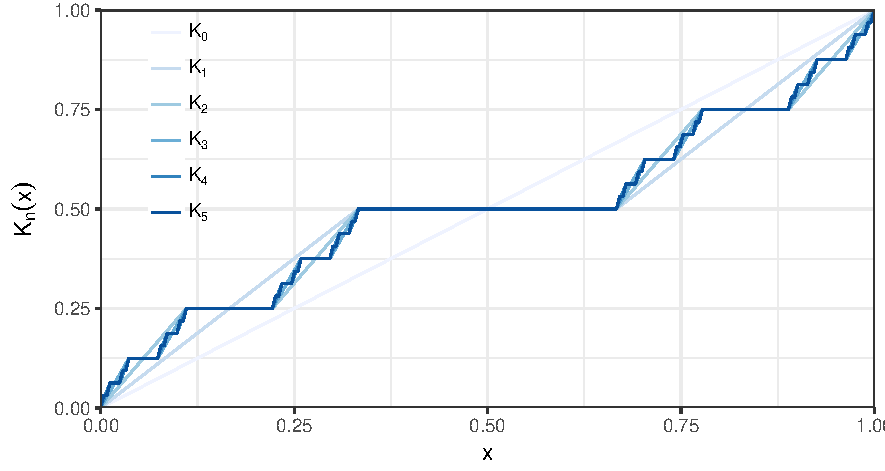
\includegraphics[width=\linewidth]{./img_mas_ejemplos/cantor.pdf}
\caption[Algunos pasos en la \textit{contrucción iterativa} de la función de Cantor]{Algunos pasos en la \textit{contrucción iterativa} de la función de Cantor, que es creciente, acotada y continua pero no absolutamente continua. En el texto, la función de Cantor es usado para construir medidas con propiedades patológicas.}
\end{figure}

%[?] demostracion de que la funcion de cantor esta bien definida
% https://es.wikipedia.org/wiki/Funci%C3%B3n_de_Cantor

\begin{proposicion}
La función de Cantor es continua pero no es absolutamente continua
\end{proposicion}

Luego entonces, puede construirse la siguiente función de distribución
\begin{equation}
F_K = \begin{cases}
K(x) &, 0\leq x \leq 1 \\
0 &, x < 0 \\
1 ,& x > 1
\end{cases}
\end{equation}
la cual no es ni continua ni discreta. Por simplicidad, en el presente trabajo únicamente se considerarán variables aleatorias que son continuas o discretas.

%La distinción entre variables aleatorias continuas y discretas puede verse más notoria en virtud del teorema \ref{Lebesgue_decomp}.

%\begin{teorema}[Descomposición de Radon-Nikodym]
%Sea $\mu$ una medida definida sobre la $\sigma$-álgebra $\mathcal{B}$, y sea $\nu$ una medida 
%$\sigma$-finita definida sobre $\mathcal{B}$. Entonces $\mu$ puede descomponerse de manera única como
%$\mu = \mu_A + \mu_S$, donde
%\begin{itemize}
%\item $\mu_A$ es absolutamente continua respecto a $\nu$
%\item Existe un conjunto $A$ tal que $\nu(A)=0$, $\mu_S\left(A^{C}\right) = 0$
%\end{itemize}
%\label{Lebesgue_decomp}
%\end{teorema}

%? pagina 109 del manual

%Dado que la medida de Lebesgue es $\sigma$-finita, cualquier medida de probabilidad puede 
%\textit{descomponerse} como la suma de una medida continua, una medida discreta y un \textit{residuo}.

\subsection{Valor esperado}

\begin{definicion}
Sea $X$ una variable aleatoria definida sobre el espacio de probabilidad $(\Omega, \mathcal{U}, P)$. Si $P$ es integrable en $\Omega$ respecto a $P$, entonces se define el \textbf{valor esperado} de $X$ como
\begin{equation}
\E{X} := \int_\omega X(\lambda) dP(\lambda)
\end{equation}
\end{definicion}

\begin{proposicion}
Sea $X$ una variable aleatoria y $g$ una función medible en el espacio edible $(\R,\mathcal{B})$. Entonces $g(X)$ es una variable aleatoria cuyo valor esperado es
\begin{equation}
\E{g(x)} = \int_\Omega [g(X)](\lambda) dP(\lambda) = \int_R g(x) dP(x)
\end{equation}
\end{proposicion}

\begin{definicion}
Sea $X$ una variable aleatoria, se definen su media $\mu_X$ y varianza $\sigma_X^{2}$ como
\begin{align}
\mu_X &{:=} \E{X} \\
\sigma_X^{2} &{:=} \E{(X-\mu_X)^{2}}
\end{align}
Por definición, no hay garantía que una variable aleatoria arbitraria tenga media o varianza bien definidas.
\end{definicion}

Naturalmente la notación $\mu_X$ únicamente se usa cuando no hay confusión con la notación para medidas. Así mismo, conviene mencionar ejemplos de varaibles aleatorias para las cuales no está bien definida su media o varianza.

? Ejemplos

%De manera más general, se define el $m$-momento de una variable aleatoria $X$ como
%\begin{equation}
%M
%\end{equation}

%\begin{definicion}
%Sea $X$ una varaible aleatoria. Se define su \textbf{función característica} como
%\begin{equation}
%\phi_X (\omega) := \E{e^{i \omega X}} = \int_\R e^{i \omega x} dF_X(x)
%\end{equation}
%donde, para todo $z\in \R$, $e^{i z} := \COS{z} + i \SEN{z}$
%\end{definicion}

\begin{definicion}
Sean $X$, $Y$ dos variables aleatorias. Se define su \textbf{covarianza} como
\begin{equation}
\Cov{X,Y} := \E{X Y} = \int_{\R^{2}} x y d P_{(X,Y)}(x,y) = \int_\R \int_\R x y dP_X(x) dP_Y(y)
\end{equation}
\end{definicion}

%\begin{proposicion}
%Si $X$, $Y$ son independientes, entonces $\Cov{X,Y} = 0$
%\end{proposicion}

\begin{definicion}
Sean $X$, $Y$ dos variables aleatorias. Se define su \textbf{coeficiente de correlación de Pearson} como
\begin{equation}
\rho (X,Y) := \sqrt{\frac{\Cov{X,Y}}{\Var{X} \Var{Y}}}
\end{equation}
\end{definicion}

%\begin{proof}
%en la pagina 65 del maual
%\end{proof}

\subsection{Vectores aleatorios}

El concepto de variable aleatoria real (definición ?) puede extenderse trivialmente a conjuntos más generales \textit{basados} en $\R$, como $\R^{n}$ para algún entero $n$; dicha generalización puede formalizarse fácilmente como otro caso particular.

\begin{definicion}
Se llama \textbf{vector aleatorio} a una variable aleatoria sobre el espacio de probabilidad $(\R^{n},\mathcal{B}^{n},P)$, para algún $n\in \N$. Se define a $\mathcal{B}^{n}$, la $\sigma$-álgebra de Borel $n$-dimensional, como
\begin{equation}
\mathcal{B}^{n} := \sigma\left(\left\{ \left(-\infty, a_1\right]\times \left(-\infty, a_2\right]\times \cdots \times \left(-\infty, a_n\right] \lvert a_1, \dots, a_n \in \R \right\}\right)
\end{equation}
\end{definicion}

Por notación, el vector aleatorio \textit{$n$-dimensional} $\boldsymbol{X}$ será referido como
\begin{equation}
\boldsymbol{X} = [X_1, X_2, \dots, X_n]
\end{equation}
esta notación para denotar vectores con \textit{símbolos gruesos} será usada durante el texto, extiendida igualmente para realizaciones y otros vectores dimilares.

\begin{ejemplo}
Se dice que un vector aleatorio $\boldsymbol{X} = [X_1, X_2, \cdots, X_d]$ sigue una \textbf{distribución multinormal} si su función de probabilidad acumulada conjunta tiene la forma
\begin{equation}
F_{\boldsymbol{X}}\left( \boldsymbol{x} \right) = \frac{1}{\sqrt{(2\pi)^{d}\abso{C}}} \exp\left( -\frac{\boldsymbol{x} C^{-1} \boldsymbol{x}^{\intercal} }{2} \right)
\end{equation}
donde $\boldsymbol{x} = (x_1, x_2, \cdots, x_d)$. El vector $\mu \in \R^{d}$ será referido como \textit{vector de medias}, y la matriz $C \in \R^{d\times d}$ como \textit{matriz de covarianza}.
\end{ejemplo}

% si se necesita, esta en la pagina 30 del manual

%%%%%%%%%%%%%%%%%%%%%%%%%%%%%%%%%%%%%%%%%%%%%%%%%%%%%%%%%%%%%%%%%%%%%%%%%%%%%%%%%%%%%%%%%%%%%%%%%%%

\section{Procesos estocásticos}

En el presente trabajo se maneja una definición muy superflua para procesos estocásticos: como una \textit{concatenación} de variables aleatorias indexadas por un conjunto $\mathcal{T} \subseteq \R$. 
%
En el libro [] se maneja una definición más formal cuya lectura es altamente recomendable; en el presente trabajo no usa tal enfoque debido a sus limitaciones y objetivos específicos.
%
Sin embargo, parece conveniente mencionarlo por comparabilidad.

Primeramente se define al conjunto $\R^{\mathcal{T}}$, de las funciones reales con dominio en $\mathcal{T}$, el cual será usado como espacio de eventos. 
%
Se pueden definir intervalos abiertos y cerrados en $\R^{\mathcal{T}}$; por ejemplo como esferas inducidas por alguna métrica, o más en concreto considerando conjuntos de la forma
\begin{equation}
B(f, R; g) = \left\{ f: \mathcal{T} \rightarrow \R \talque \int_{\mathcal{T}} \abso{f(x)-g(x)} dx < R \right\}
\end{equation}

En general, habiendo definido una colección \textit{suficientemente buena} de conjuntos se puede definir inmediatamente la $\sigma$-álgebra definida por dicha familia.
%
Finalmente, basta definir una medida sobre la $\sigma$-álgebra mencionada.

Escribir un proceso estocástico como variable aleatoria facilita algunas \textit{tareas}, como definir sus realizaciones y hablar sobre límites de procesos estocásticos. 
%
Por oto lado, ello dificulta tareas como construir procesos procedimentalmente, definir la autocovarianza y hablar sobre muestreo.
%
Bajo este comentario, escribir un proceso estocástico como concatenación de variables aleatorias es un enfoque intuitivamente contrario, pues \textit{invierte} las ventajas y desventajas.

\begin{definicion}
Un \textbf{proceso estocástico} \xt es una colección de variables aleatorias indexadas por el símbolo $t\in\mathcal{T}$
%\begin{equation}
%\{X(t)\}_{t\in \mathcal{T}} := \left\{ X(t) \lvert t\in \mathcal{T} \right\}
%\end{equation}
\end{definicion}

\begin{definicion}
Se dice que un proceso estocástico \xt es un \textbf{proceso estocástico en $\R$} si cumple que $\mathcal{T} \subseteq \R$.
%
Por notación, el índice $t$ es referido como \textbf{tiempo}, mientras que $\mathcal{T}$ es el conjunto de \textbf{tiempos admisibles}.
\end{definicion}

Por simplicidad sobre las condiciones del presente trabajo, sólo se trabajará con dos familias de procesos estocásticos en $\R$: si $\mathcal{T}$ es un intervalo, o si es parte de una \textit{malla}. 
%
La primera familia se reserva para modelar las señales electrofisiológicas per se, mientras que el segundo se usa para modelar los registros de estas mismas señales.
%
La distinción consiste en que las señales sólo pueden ser registradas digitalmente en un conjunto finito de puntos; ambos grupos merecen atención, y se espera que sus características sean similares.

\begin{definicion}
Se dice que un proceso estocástico en $\R$ es \textbf{a tiempo continuo} si existen $a, b \in \R \cup \{ -\infty, \infty \}$ tales que
\begin{equation}
\mathcal{T} = (a,b)
\end{equation}
Así mismo, se dice que un proceso estocástico en $\R$ es \textbf{a tiempo discreto} si existen $t_0, \Delta_X \in \R \cup \{ -\infty, \infty \}$ tales que
\begin{equation}
\mathcal{T} = \left\{ t_0 + t \in \R \talque {t} \cdot {\Delta_X} \in \Z \right\}
\end{equation}
Por notación, $\Delta_X$ es referida como \textit{frecuencia de muestreo}.
\end{definicion}

Conviene destacar que el nombre \textit{frecuencia de muestreo} hace referencia al proceso de registro, que algunos autores usan como equivalente a \textit{muestreo}; esta terminología entra claramente en conflicto con las muestras de una variable aleatoria. En lo siguiente se evita llamar muestreo al proceso de registro, pero se conservará el término frecuencia de muestro.

Cabe mencionar una cuestión similar con los términos \textit{tiempo continuo} y \textit{tiempo discreto}; cabe resaltar que \underline{no guardan ninguna analogía} con las variables aleatorias discretas y continuas, ni con los espectro de potencias puramente continuos o puramente discretos (ver el capítulo siguiente).
%
El uso de estos términos se debe principalmente a que se encuentran ampliamente extendidos en la literatura sobre análisis de señales.

Para evitar confusiones, los elementos que componen a un proceso estocástico son denotados como:\\
\begin{tabular}{cl}
\xt    & Todo el proceso \\
$X(t)$ & Variable aleatoria en el proceso, para el tiempo $t$ \\
$x(t)$ & Una realización de $X(t)$ \\
$F_{X(t)}$ & Función de probabilidad acumulada para $X(t)$
%$ {\Delta_t}$ & Frecuencia de muestreo (en tiempo discreto)
\end{tabular}\\

La estacionariedad es un indicativo de la \textit{homogeneidad} de un proceso; un proceso 
\textit{muy} estacionario sería aquél cuyas variable aleatoria que tiene distribuciones conjuntas que no cambian 
con el tiempo. 
%
La definición \ref{est_fuerte} representa con exactitud tales requerimientos, pero se le considera 
\textit{innecesariamente fuerte}; una definición común es \ref{est_m}.

\begin{definicion}[Estacionariedad fuerte]
Un proceso \xt se dice fuertemente estacionario si para cualesquiera 
$t_1, t_2, \dots, t_n \in \mathcal{T}$ y cualquier $\tau$ tal que $t_i + \tau \in \mathcal{T}$,
se cumple que
\begin{equation*}
F_{\left[ X(t_1), X(t_2), \dots, X(t_n) \right]} \equiv
F_{\left[ X(t_1 + \tau), X(t_2 + \tau), \dots, X(t_n + \tau) \right]}
\end{equation*}
Donde $F_{[v_1,v_2,\dots,v_N]}$ es la FPA conjunta para el vector $[v_1,v_2,\dots,v_N]$
\label{est_fuerte}
\end{definicion}

\begin{definicion}[Estacionariedad de orden $m$]
Un proceso \xt se dice estacionario de orden $m$ si, para cualesquiera
$t_1, t_2, \dots, t_n \in \mathcal{T}$ y cualquier $\tau$ tal que $t_i + \tau \in \mathcal{T}$,
se cumple que
\begin{equation*}
\E{X^{m_1}(t_1)X^{m_2}(t_2)\cdots X^{m_n}(t_n)} =
\E{X^{m_1}(t_1+\tau)X^{m_2}(t_2+\tau)\cdots X^{m_n}(t_n+\tau)}
\end{equation*}
para cualesquiera enteros $m_1, m_2, \dots, m_n$ tales que $m_1+m_2+\cdots+m_n \leq m$
\label{est_m}
\end{definicion}

Cabe mencionar que la definición \ref{est_m} no es equivalente a la definición \ref{est_fuerte}, ni
aún cuando $m\rightarrow \infty$; sin embargo permite asegurar que los \textit{momentos} 
($\E{X^{k}}$ para algún $k$) del proceso sean invariantes en el tiempo, y éstos suelen encontrarse
asociados a cantidades físicas.

Como un ejemplo muy particular conviene destacar la energía, que suele ser asociada con el segundo
momento (definición \ref{energia}). 
%
Dicha conexión motiva a escoger una definición de estacionariedad que permita analizar la energía 
del proceso: la estacionariedad débil.

\begin{definicion}[Estacionariedad débil]
Un proceso \xt se dice débilmente estacionario si existen constantes $\mu, \sigma \in \R$ y una 
función $R : \mathcal{T} \rightarrow \R \cup \{ \pm \infty \} $ tales que, para cualesquiera $t, s \in T$ se 
cumple
\begin{itemize}
\item $\E{X(t)} = \mu$
\item $\Var{X(t)} = \sigma^{2}$
\item $\Cov{X(t),X(s)} = R(s-t)$
\end{itemize}
\end{definicion}

\begin{figure}
\centering
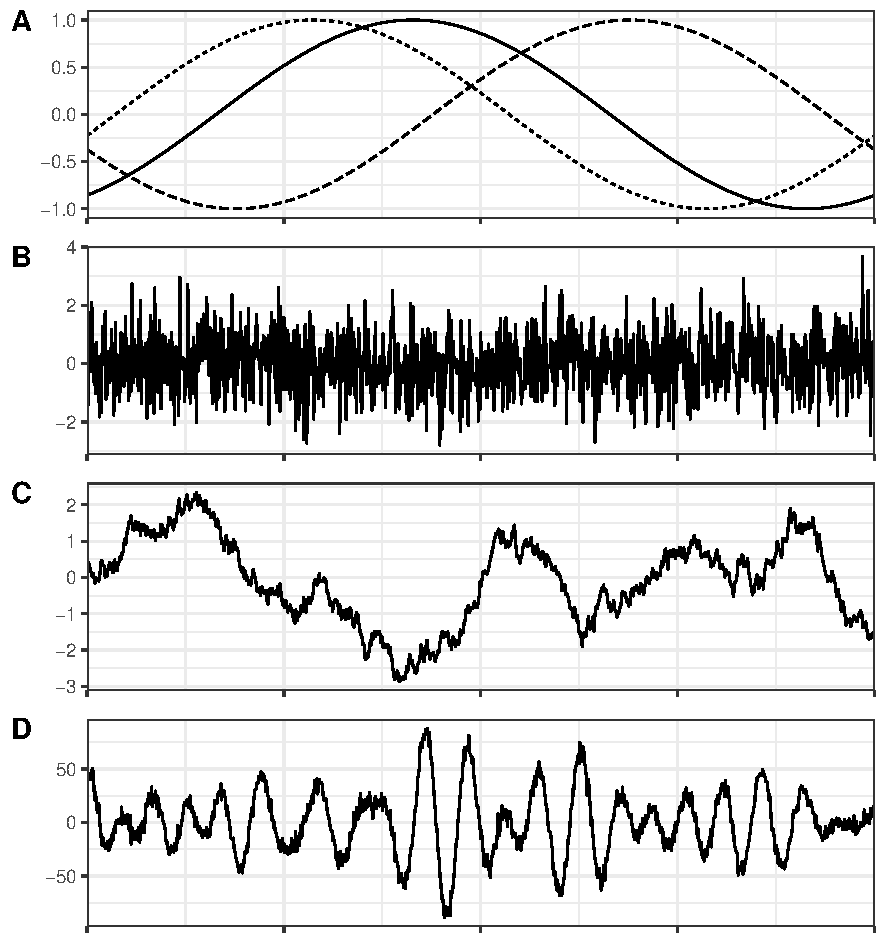
\includegraphics[width=\linewidth]{./img_mas_ejemplos/ruidos_ejemplos.pdf}
\caption[Realizaciones de algunos proceos débilmente estacionarios]{Realizaciones de algunos procesos débilmente estacionarios. \textbf{A.} Proceso oscilante, del cual se grafican tres realizaciones diferentes. \textbf{B.} Proceso ruido blanco. \textbf{C.} Proceso de medias móviles (MA). \textbf{D.} Proceso tipo alfa. \textbf{E.} Proceso ruido rosa.}
\end{figure}

\begin{proposicion}
Un proceso estocástico es débilmente estacionario si y sólo si es estacionario de orden 2.
\end{proposicion}

La proposición anterior deja en claro que la estacionariedad débil puede entenderse como una \textit{estabilidad} en los momentos conjuntos de orden al menos dos, condición suficiente para trabajar con la media y la varianza del proceso.
%
Sin embargo, en ocasiones se requerirán condiciones más fuertes sobre los procesos. Como ejemplo, cuando se quiere obtener la varianza para un estimador del espectro de potencias, se necesita que la serie sea estacionaria de orden 4. 

%Cabe destacar que la estacionariedad débil no sólo tiene como condición que todas las variables del
%proceso tengan la misma media y varianza, sino que también supone que éstas son finitas.
%
%Sobre la función de covarianza $R$ (que en un único proceso es referida como \textit{autocovarianza}),
%no hay restricciones sobre los valores que pueda tomar, excepto que 
%$R(0) = \Var{X(\bullet)} < \infty$. 
%%
En el marco del modelo de series electrofisiológicas, conviene suponer que los registros 
corresponden a procesos a tiempo continuo que son continuos de alguna forma; se ha elegido la 
continuidad en media cuadrática.

Cuando una señal electrofisiológica se modela como un proceso estocástico, es necesario suponer que su media y varianza son finitas en todo momento. 
%
Esto se debe a que existen umbrales \textit{naturales} en los que ocurren las mediciones, fuera de los cuales la vida misma es imposible; este comentario aplica también sobre la energía dentro del sistema.
%
Más aún, la actividad eléctrica cerebral y muscular presentan una actividad característica del estado de reposo (\textit{actividad basal}) de la cual no se \textit{alejan mucho} el resto del tiempo; esta suerte de media intuitiva es referida como \textit{línea base}, y se refleja dentro del modelado con la insistencia heurística de tratar a los procesos como si tuvieran media cero.

\begin{observacion}
Sea \xt un proceso débilmente estacionario y $R$ su función de autocovarianza. Si $R$ es continua
en 0 entonces es continua en todo $\R$.
\end{observacion}

\begin{definicion}[Continuidad estocástica en media cuadrática]
Un proceso a tiempo continuo \xt es estocásticamente continuo, en el sentido de media cuadrática, 
en un tiempo admisible $t_0$ si
\begin{equation*}
\lim_{t \rightarrow t_0} \E{\left( X(t) - X(t_0) \right)^{2}} = 0
\end{equation*}
\label{cont_est}
\end{definicion}

%Una forma natural de pensar en la definición \ref{cont_est} es que si $\abso{t-t_0}$ es muy pequeño 
%entonces $X(t)$ y $X(t_0)$ difieren muy poco entre sí, como variables aleatorias.
%%
%Hablando de procesos débilmente estacionarios, la continuidad estocástica de un proceso es 
%equivalente a que su función de autocovarianza sea continua en 0.

\begin{proposicion}
Sea \xt un proceso a tiempo continuo y débilmente estacionario, y sea $R$ su función de autocovarianza. El proceso es estocásticamente continuo si y sólo si $R$ es continua en 0.
\end{proposicion}

%%%%%%%%%%%%%%%%%%%%%%%%%%%%%%%%%%%%%%%%%%%%%%%%%%%%%%%%%%%%%%%%%%%%%%%%%%%%%%%%%%%%%%%%%%%%%%%%%%%

\section{Estimación de parámetros}

Es común que se conozca cierta información de estos fenómenos que permita suponer que se comportan como variables aleatorias con cierta forma. Por ejemplo, ?.%se suele suponer que entre la población, 
%
Conviene destacar el caso de fenómenos que son \textit{forzados} a seguir una distribución conocida; por ejemplo, la metodología para aplicar la prueba Neuropsi \cite{Ostrosky00} ha sido diseñada de tal forma que los puntajes siguen una distribución normal para cada segmento poblacional.

En este tipo de escenarios se puede hablar de una función de distribución $f(\bullet; \theta)$ que depende de un parámetro $\theta \in \Omega$, donde $\Omega$ se conoce como \textbf{espacio de parámetros}; el objetivo consiste en deducir el valor de $\theta$ a partir de los datos recabados.

\begin{definicion}
Sea $X$ una variable aleatoria. Una \textbf{muestra de $X$ de tamaño $N$} es una colección de variables aleatorias $\{ X_1, X_2, \dots, X_N \}$ tales que son independientes y que comparten la misma distribución de $X$
\end{definicion}

\begin{proposicion}
Sea $X$ una variable aleatoria que admite una función de densidad $f_X$, y sea $\{ X_1, X_2, \dots, X_N \}$ una muestra. La función de densidad de probabilidad conjunta para el vector $[ X_1, X_2, \dots, X_N ]$ es
\begin{equation}
f_{[ X_1, \dots, X_N ]}(x_1, \dots, x_N ) = \prod_{j=1}^{N} f(x_j)
\end{equation}
Mientras no se indique lo contrario, las variables aleatorias en la muestra no están ordenadas.
\end{proposicion}

\begin{proposicion}
Sea $X$ una variable aleatoria, $\{ X_1, X_2, \dots, X_N \}$ una muestra y $\{ x_1, x_2, \dots, x_N \}$ un conjunto de observaciones. Se define la \textbf{función de distribución muestral} como
\begin{equation}
F_{X; N} (x) := \frac{1}{N} \sum_{x_j \leq x } 1
\end{equation}
\end{proposicion}

\begin{proposicion}
Si el tamaño de una muestra de $X$ se vuelve arbitrariamente grande, la función de distribución muestral converge en probabilidad a $F$, la función de probabilidad acumulada de $X$
\begin{equation}
\lim_{N \rightarrow \infty} F_{X; N} = F_X
\end{equation}
\end{proposicion}

%\begin{proof}
%Ver seccion 5.2 C R Rao, Linear Statistic Inference and its applications 2 ed pag 42
%\end{proof}

\begin{definicion}
Un \textbf{estadístico} es una función de las observaciones en una muestra
\end{definicion}

Ejemplo en pagina 112 del libro de lindgren.
Si $X\sim N(\mu,\sigma^{2})$, sea $\overline{X} = \frac{1}{N} \sum X_j$, entonces
\begin{equation}
\overline{X} \sim N(\mu,\frac{\sigma^{2}}{N})
\end{equation}

\begin{teorema}[Cramér-Rao]
Sea $\widehat{\theta}$ un estimador insesgado de $\theta$. Si la función de verosimilitud asociada al estimador, $L$, es diferenciable, entonces
\begin{equation}
\Var{\widehat{\theta}} \geq \left( \E{\frac{\partial}{\partial\theta} L(X; \theta)} \right)^{-2}
\end{equation}
La igualdad se alcanza si y sólo si existe una función positiva $k$ tal que puede escribirse
\begin{equation}
\frac{\partial}{\partial\theta} L(X; \theta) = k(\theta) \left[ \widehat{\theta}(X) - \theta \right] 
\end{equation}
\end{teorema}


%Ejemplo.
%Considérese la variable aleatoria binomial $X \sim B(\theta)$ con $\theta \in [0, 1]$, cuya FDP es
%\begin{equation}
%f_X(x; \theta) = \begin{cases}
%\theta^{x} (1-\theta)^{1-x} &, x\in \{ 0,1 \} \\
%0 &, \text{otro caso}
%\end{cases}
%\end{equation}
%La FDP conjunta para una muestra de tamaño $N$ es
%\begin{equation}
%f_N(x_1, \dots, x_N; \theta) = 
%\begin{cases}
%\theta^{\sum_i x_i}(1-\theta)^{\sum_i(1-x_i)} &, x_i \in \{ 0,1 \}, i\in \{1, \dots, N\} \\
%0 &, \text{otro caso}
%\end{cases}
%\end{equation}
%
%Se puede entender a $f_N$, evaluada en los datos obtenidos y como función de $\theta$, como la probabilidad de que se hayan obtenido los datos que de hecho se obtuvieron.
%%
%Esta redundancia sugiere que una elección adecuada para el parámetro $\theta$ sería aquél que maximice a tal función, que que recibe el nombre de \textbf{función de verosimilitud}
%\begin{equation}
%L(\theta; x_1, \dots, x_N) = \theta^{\sum_i x_i}(1-\theta)^{\sum_i(1-x_i)}
%\end{equation}
%con $\theta \in [0, 1]$. Por simplicidad técnica, se maximizará a $L$ igualando a cero la derivada de $\log \circ L$ con respecto a $\theta$.
%\begin{align*}
%\frac{d}{d\theta} \log\left( L(\theta; x_1, \dots, x_N)\right)
%&= 
%\frac{d}{d\theta} \log\left(\theta^{\sum_1^{N} x_i}(1-\theta)^{\sum_1^{N}(1-x_i)}\right) \\
%&=
%\frac{d}{d\theta} \left[ \left( \sum_{1}^{N} x_i \right) \log(\theta) + 
%\left( \sum_{1}^{N}(1-x_i) \right) \log (1-\theta)\right] \\
%&= \left( \sum_{i=1}^{N} x_i \right) \frac{1}{\theta} -
%\left( N - \sum_{i=1}^{N}(x_i) \right) \frac{1}{1-\theta}
%\end{align*}
%
%Luego entonces, la función de verosimilitud es maximizada usando $\theta = \frac{1}{N} \sum_{1}^{N}(x_i)$.

\begin{definicion}
Sea $X$ una variable aleatoria que depende de un parámetro $\theta$ y $X_1, \dots, X_N$ una muestra de tamaño $N$. Un estimador $\widehat{\theta}$ es \textbf{suficiente} si
la distribución de la variable $X \lvert \widehat{\theta}$ no depende de $\theta$
\end{definicion}

\begin{teorema}
Sea $X$ una varaible aleatoria que depende del paraámetro $\theta$. Un estadístico $\widehat{\theta}$ es suficiente si y sólo si existen funciones $g$ y $h$ tales que
\begin{equation}
f_X(\bullet; \theta ) = g(\widehat{\theta},\theta) h_X(\bullet)
\end{equation}
\end{teorema}

%\begin{proof}
%ver pagina 121 del libro de lindgren
%\end{proof}

%El \textbf{espacio de datos} es 

%Usando la desigualdad de Chebyshev de puede deducir que
%\begin{equation}
%P\left( \abso{\widehat{\theta} - \theta} > \varepsilon \right) \leq 
%\frac{1}{\varepsilon^{2}} \E{\left( \widehat{\theta} - \theta \right)^{2}}
%\end{equation}

\begin{definicion}
El \textbf{error de media cuadrática} para el estimador $\widehat{\theta}$ se define como
\begin{equation}
\text{EMC}(\widehat{\theta}) := \E{\left( \widehat{\theta} - \theta \right)^{2}} =
\Var{\widehat{\theta}} + \left( \E{\theta} - \theta^{2} \right)
\end{equation}
\end{definicion}

\begin{definicion}
Sea $X$ una variable aleatoria que depende de un parámetro $\theta$ y $X_1, \dots, X_N$ una muestra de tamaño $N$. Un estimador $\widehat{\theta}$ es \textbf{insesgado} si cumple que
\begin{equation}
\E{\widehat{\theta}} = \theta
\end{equation}
\end{definicion}

Se puede hablar del \textbf{sesgo} del estimador $\widehat{\theta}$ como $\E{\widehat{\theta}}-\theta$

\begin{definicion}
Sea $X$ una variable aleatoria que depende de un parámetro $\theta$ y $\left\{ \widehat{\theta}_n \right\}_{n\in \N}$ una familia de estimadores definidos para muestras de $X$ de tamaño arbitrario. La familia de estimadores se dice \textbf{consistente} si para cualquier $\varepsilon > 0$
\begin{equation}
\lim_{n\rightarrow\infty} P\left( \abso{\widehat{\theta}_n-\theta} > \varepsilon \right) = 0
\end{equation}
\end{definicion}

\begin{definicion}
Así como en la definición anterior, se dice que a familia de estimadores \textit{converge en media cuadrática} si
\begin{equation}
\lim_{n\rightarrow\infty} \E{\left( \widehat{\theta}_n - \theta \right)^{2}} = 0
\end{equation}
Si esto se cumple, se dice que la familia de estimadores es \textbf{consistente en media cuadrática} \end{definicion}

\begin{proposicion}
Si $\widehat{\theta}_n$ es una familia de estimadores consistente en media cuadrática, entonces es consistente
\end{proposicion}

\begin{proposicion} COROLARIO
Una condición suficiente para para que una familia sea consistente en en media cuadrática es
\begin{align}
\lim_{n\rightarrow\infty} \E{\widehat{\theta}_n} &= \theta \\
\lim_{n\rightarrow\infty} \Var{\widehat{\theta}_n} &= 0
\end{align}
\end{proposicion}

%\begin{proof}
%? pag 141 del libro de lindgren
%\end{proof}

\begin{teorema}[Límite central]
Sea $\{ X_1, \cdots, X_N\}$ una muestra de tamaño $N$ de una variable aleatoria con distribución normal, $X\sim N(\mu,\sigma^{2})$. Defínase la variable aleatoria $Y_N$ como
\begin{equation}
Y_N = \frac{\sum_{i=1}^{N}X_i - N \mu}{\sqrt{N \sigma^{2}}}
\end{equation}
Entonces $\{ Y_N \}_{N \in \N}$ converge en probabilidad a una distribución normal $N(0,1)$.
\end{teorema}

%%%%%%%%%%%%%%%%%%%%%%%%%%%%%%%%%%%%%%%%%%%%%%%%%%%%%%%%%%%%%%%%%%%%%%%%%%%%%%%%%%%%%%%%%%%%%%%%%%%

\section{Pruebas de hipótesis}

%? empieza en la pagina 156 del libro de lindgren

Una hipótesis es una afirmación sobre algún aspecto desconocido.
%
Es tarea común en la estadística el decidir si alguna afirmación puede sostenerse a partir de la
información proporcionada por un conjunto de observaciones. 
%
A partir de la aplicación masiva de pruebas neuropsicológicas a un grupo de adultos mayores uno 
puede preguntarse, por ejemplo, si hombres y mujeres tienden a obtener puntajes diferentes en las
pruebas, o si la edad de los participantes está correlacionada con su desempeño en tareas de 
memoria.
%
En la tabla ... se muestran los datos sobre una simulación (artificial) de dicho escenario.

Una herramienta de uso común para producir estas decisiones es la \textbf{pruebas de hipótesis},
la cual consiste en dos afirmaciones complementarias, es decir, tales que exactamente una de ellas es verdadera; tales afirmaciones
son referidas como \textit{hipótesis}, y deben elegirse de forma que sean equivalentes a la 
decisión que se busca. 
%
Usualmente la primera de las hipótesis (hipótesis nula, $H_0$) representa la afirmación más general o que se cree verdadera por omisión, mientras que la segunda hipótesis (hipótesis alternativa, $H_A$) se tomará como verdadera si
existe suficente información para rechazar la veracidad de la primera.
%
%La idea intuitiva detrás de las pruebas estadísticas es que una muestra de la población se comporta de manera similar a la población.
%
El enfoque de prueba de significancia es  tomar un estadístico $\est{\theta}$ y evaluarlo sobre los datos, posteriormente se analiza qué tan diferente es el valor obrevado del típico cuando la hipótesis nula es verdadera.

Los estadísticos de prueba suele ser un estadístico construido para tener una distribución conocida salvo unos pocos parámetros fáciles de estimar.
%
La interpretación usual es que, si $H_0$ es verdadera entonces $\est{\theta}$ puede no tener el valor predicho debido a factores ajenos al fenómeno estudiado, en consecuencia se suele hablar de una región de rechazo en el espacio de estados (ver más adelante).
%
Bajo esta interpretación, un valor de $\widehat{\theta}$ dentro de la región de rechazo significa que los datos representan evidencia para rechazar $H_0$; un no-rechazo no significa precisamente que $H_0$ sea verdadera, sino que las observaciones no representan evidencia suficiente para rechazar $H_0$.

\begin{definicion}
En una prueba de hipótesis, rechazar $H_0$ cuando es verdadero es un \textbf{error del tipo I}. Así msimo, aceptar $H_0$ cuando es falsa es un \textbf{error del tipo II}.
\end{definicion}

La naturaleza e intepretación de los estadísticos de prueba suelen ser muy particulares de las situaciones bajo las cuales son definidos.
%
Una forma típica de normalizar los diferentes estadísticos es a través del $p$-valor, definido como la probabilidad de que ocurra un valor extremo del estadístico de prueba; 
el $p$-valor suele interpretarse como la \textit{fuerza} de la evidencia contra $H_0$.

\begin{definicion}
Sea $\widehat{\theta}$ un estadístico de prueba. El \textbf{$\boldsymbol{p}$-valor} asociado al $\widehat{\theta}=\theta_0$ es la probabilidad $P\left(\widehat{\theta}\right>\theta_0)$
\end{definicion}

Una \textbf{prueba de sinificancia} se entiende como una pruebas de hipótesis para algunos $p$-valores predefinidos, usualmente 0.05, 0.01, 0.005, entre otros.
%
Un error común, pero muy extendido, es interpretar al $p$-valor como la probabilidad de obtener $H_0$.

\begin{definicion}
Dada una muestra poblacional y dos afirmaciones complementarias $H_0$ y $H_A$, una \textbf{prueba de hipótesis} es una regla de decisión que asigna a cada punto del espacio de estados una acción del conjunto Aceptar $H_0$, rechazar $H_A$, Rechazar $H_0$, aceptar $H_A$.

Al conjunto del espacio muestral sonde se rechaza $H_0$ se le denomina \textbf{región crítica}. 
\end{definicion}

%\begin{definicion}
%La función de potencia es el supremo, sobre todas las distribuciones muestrales, de la probabilidad de que una muestra
%\end{definicion}

%Por comodidad, uno puede redefinir a la región crítica en términos del estimador $\widehat{\theta}$. 
Una propiedad deseable para un estadístico de prueba es poder acotar los errores de tipo I y de tipo II; para ello, para alguna región crítica arbitraria $\mathcal{C}$ se define el \textbf{nivel de significancia} de la prueba como
\begin{equation}
\alpha := \sup_{\theta \in H_0} p(\mathcal{C} \lvert \theta)
\end{equation}

Ejemplo:
Retomando los datos de la tabla ..., considérese la pregunta \textit{¿Los hombres y mujeres tienden
a obtener puntajes diferentes en las pruebas neuropsicológicas?}. 
%
En este ejemplo se supone que los puntajes de los hombres en la prueba siguen una distribución normal con media $\mu_H$ y varianza 1, y similarmente para las mujeres con media $\mu_M$ y varianza 1.
%
Como hipótesis nula se elige la posibilidad de que en promedio ambos grupos (hombre y mujeres) obtengan el mismo puntaje en la prueba, es decir
\begin{equation}
H_0 : \mu_H = \mu_M
\end{equation}
y como hipótesis alternativa está la posibilidad de que los puntajes sean diferentes
\begin{equation}
H_A : \mu_H \neq \mu_M
\end{equation}

%\subsection{Clasificación de dos vías}
%
%Un \textbf{diseño aleatorio por bloques} es un muestreo aleatorio en varias categorías de sujetos 

%%%%%%%%%%%%%%%%%%%%%%%%%%%%%%%%%%%%%%%%%%%%%%%%%%%%%%%%%%%%%%%%%%%%%%%%%%%%%%%%%%%%%%%%%%%%%%%%%%%
%%%%%%%%%%%%%%%%%%%%%%%%%%%%%%%%%%%%%%%%%%%%%%%%%%%%%%%%%%%%%%%%%%%%%%%%%%%%%%%%%%%%%%%%%%%%%%%%%%%

\section{Espacios de Hilbert}

\section{Transformada de Fourier}
\label{sec:fourier1}

Para exponer formalmente lo que es la transformada de Fourier, conviene mencionar los espacios de 
las \textbf{series $\boldsymbol{p}$-sumables} ($\lp$), y las  \textbf{funciones 
$\boldsymbol{p}$-integrables} sobre un intervalo $I \subseteq \R$ ($\llp_I$).
\begin{align*}
\ell^{p} &:= \left\{ s: \Z\rightarrow\C \talque \sum_{n=-\infty}^{\infty} \abso{s(n)}^{p} < \infty \right\}
\\
L^{p}_I &:= \left\{ S: I\rightarrow\C \talque \int_I \abso{S(t)}^{p} dt < \infty \right\}
\end{align*}

Estos conjuntos admiten las operaciones  suma ($+$), producto ($\cdot$) y multiplicación por 
escalares de la manera usual.
%
Para el caso particular $p=2$, los conjuntos $\ldos$ y $\lldos$ admiten los siguientes productos 
internos:
%
\begin{align*}
\left\langle s,z \right\rangle &= \sum_{n=-\infty}^{\infty} s(n) \overline{z(n)}\\
\left\langle S,Z \right\rangle &= \int_I S(t) \overline{Z(t)} dt
\end{align*}

Usando dichos productos internos, junto con las normas y métricas que inducen, los conjuntos 
$\ldos$ y $\lldos$ tienen estructura de \textit{espacio de Hilbert}.

Las definiciones anteriores revelan cómo $\ldos$ y $\lldos$ son \textit{muy} parecidos, luego
entonces se puede definir la transformada de Fourier como una conexión natural entre ellos.

\begin{definicion}[Serie de Fourier]
Sea $S: \R \rightarrow \C$ una función periódica con periodo $2T$ y tal que 
$S \in L^{2}_{[-T,T]}$. Se dice que $A$ es la serie de Fourier para $S$ si satisface
\begin{equation*}
A(n) = \frac{1}{2 T} \simint{T} S(t) e^{-\nicefrac{ i \abso{n} t}{2T}} dt
\end{equation*}
\label{FourierClasico}
\end{definicion}

\begin{definicion}[Transformada de Fourier]
Sean $S$ y $A$ como en la definición \ref{FourierClasico}. Se le llama transformada de Fourier a la
función $\mathcal{F}_T : L^{2}_{[-T,T]} \rightarrow \ldos : S \mapsto A$
\end{definicion}

Puede interpretarse a $A$ como las \textit{coordenadas} de $S$ en $L^{2}_{[-T,T]}$, usando una base 
de funciones ortonormales $\left\{ e^{\nicefrac{i \abso{n} t}{2 T}} \right\}_{n\in \Z}$; esta base 
en particular es conocida como la \textbf{base de Fourier}.
%
Cabe mencionar las siguientes propiedades de $\mathcal{F}_T$
\begin{itemize}
\item Es lineal, $\mathcal{F}_T[cS + Z] = c\mathcal{F}_T[S] + \mathcal{F}_T[Z]$

\item \textbf{No} es invertible, aunque se le suele definir una pseudoinversa como
\begin{equation*}
\mathcal{F}_{T}^{\text{inv}} : \ldos \rightarrow L^{2}_{[-T,T]} :
A \mapsto \sum_{n -\infty}^{\infty} A(n) e^{\nicefrac{i \abso{n} t}{2 T}}
\end{equation*}
\end{itemize}

Se define, de manera pragmática, la \textbf{energía disipada} y la \textbf{potencia} de una función 
$S$ en un intervalo $[a,b]$ como 
\begin{align}
\text{energía}[S]_{[a,b]} &= \int_a^{b} \abso{S(t)}^{2} dt \nonumber \\
\text{potencia}[S]_{[a,b]} &= \frac{1}{b-a} \int_a^{b} \abso{S(t)}^{2} dt
\label{energia}
\end{align}

Es evidente que la energía y potencia están relacionadas a la norma en $L^{2}_{[-T,T]}$ inducida por
su producto interno.
%
Dicha relación junto a las propiedades \textit{agradables} de $\mathcal{F}_T$ pueden ser usadas 
para conectar la energía con la norma en $\ldos$ (teorema \ref{parseval}): la energía disipada por 
una función equivale a la suma de las energías disipada por cada una de sus \textit{componentes} en 
la base de Fourier.
%
Conviene, entonces, definir una función que \textit{desglose} estos \textit{aportes}.

\begin{teorema}[Parseval]
Sea $S \in L^{2}_{[-T,T]}$, y sea $A = \mathcal{F}[S]$. Se cumple que
\begin{equation*}
\int_{-T}^{T} \abso{S(t)}^{2} dt = \sum_{n=-\infty}^{\infty} \abso{A(n)}^{2}
\end{equation*}
\label{parseval}
\end{teorema}

%\begin{definicion}[Espectro de potencias]
%Sea $S \in L^{2}_{[-T,T]}$, y sea $A = \mathcal{F}[S]$. Se llama espectro de potencias 
%para $S$ a la función $h_S : \R \rightarrow \R $, definida como
%\begin{equation*}
%h_S(\omega) = 
%\begin{cases}
%\abso{A(n)}^{2} & \text{ , si } \omega = \nicefrac{n}{2T}, \text{   con } n\in \mathbb{Z} \\
%0 & \text{ ,  otro caso}
%\end{cases}
%\end{equation*}
%\label{espec}
%\end{definicion}

Un elemento que será de crucial importancia en el desarrollo posterior es la \textbf{convolución} 
($\ast$), una tercera operación binaria en estos espacios y definida como
%
\begin{align*}
[s \ast z] (\tau) &= \sum_{n=-\infty}^{\infty} s(n) \overline{z(\tau-n)} \\
[S \ast Z] (\tau) &= \int_I S(t) \overline{Z(\tau-t)}
\end{align*}
%
donde $\overline{c}$ es el conjugado complejo de $c$. 
%
%Esta operación cobra importancia por la forma en que se relaciona con $\mathcal{F}_T$
%%
%\begin{observacion}%[de la convolución]
%Sean $S,Z \in L^{2}_{[-T,T]}$, entonces se satisface que
%\begin{align*}
%\mathcal{F}_T[S\ast Z]  &= \mathcal{F}_T[S] \cdot \mathcal{F}_T[Z] \\
%\mathcal{F}_T[S\cdot Z] &= \mathcal{F}_T[S] \ast  \mathcal{F}_T[Z] 
%\end{align*}
%\label{t_convolucion}
%\end{observacion}

\begin{teorema}
Sean $f, g \in \ldos$, las cuales poseen una transformada de Fourier de la forma
\begin{align*}
F(\omega) = \intR e^{-i \omega t} f(t) dt \\
G(\omega) = \intR e^{-i \omega t} g(t) dt 
\end{align*}
Entonces
\begin{equation}
F(\omega) \overline{G(\omega)} = \intR e^{i \omega t} k(t) dt
\end{equation}
donde
\begin{equation}
k(t) = \intR f(u) g(u-t) du
\end{equation}
\end{teorema}

\begin{proof}
Nótese que
\begin{align*}
\intR e^{i \omega t} k(t) dt &= \intR e^{i \omega t} \left[ k(t) = \intR f(u) g(u-t) du \right] dt \\
&= \intR e^{-i \omega u} f(u) \left[ \intR e^{i \omega (u-t)} g(u-t) \right] du \\
&= \intR e^{-i \omega u} f(u) \overline{G(\omega)} du \\
&= \overline{G(\omega)} \intR e^{-i \omega u} f(u)  du \\
&= \overline{G(\omega)} F(\omega) \\
\end{align*}
\end{proof}

\begin{align*}
[s \ast z] (\tau) &= \sum_{n=-\infty}^{\infty} s(n) \overline{z(\tau-n)} \\
[S \ast Z] (\tau) &= \int_I S(t) \overline{Z(\tau-t)}
\end{align*}

\begin{teorema}
COROLARIO. Usando $f \equiv g$ en el teorema anterior
\begin{equation}
\abso{F(\omega)}^{2} = \intR e^{- i \omega t} k(t) dt 
\end{equation}
donde 
\begin{equation}
k(t) = \intR f(u) f(u-t) du
\end{equation}
\end{teorema}

%%%%%%%%%%%%%%%%%%%%%%%%%%%%%%%%%%%%%%%%%%%%%%%%%%%%%%%%%%%%%%%%%%%%%%%%%%%%%%%%%%%%%%%%%%%%%%%%%%%
%%%%%%%%%%%%%%%%%%%%%%%%%%%%%%%%%%%%%%%%%%%%%%%%%%%%%%%%%%%%%%%%%%%%%%%%%%%%%%%%%%%%%%%%%%%%%%%%%%%

\section{Otros resultados importantes}

Los siguientes teoremas y proposiciones se refieren a propiedades únicamente de los objetos descritos en el capítulo.
%
Aunque no son una consecuencia clara de los resultados expuestos anteriormente, son una base importante de algunos resultados que se expondrán en capítulos posteriores.

El teorema de Isserlis es una identidad relativamente poco conocida sobre los cuartos momentos de una distribución multinormal; el caso particular de cuatro variables será usado para calcular la covarianza de algunos estimadores del espectro de potencias.

\begin{proposicion}
Sea $g$ una función cuando menos dos veces derivable cuyo dominio es $\mathcal{D}_g$, y sea $X$ una variable aleatoria real tal que $P(X\notin \mathcal{D}) = 0$. 
%Si los momentos de $X$ están acotados y la secuencia $\left\{ \frac{1}{n !} \frac{d^{n}}{dx^{n}} g\left( \E{X} \right) \right\}$ está acotada, entonces 
Pueden usarse las siguientes aproximaciones
\begin{align}
\E{g(X)} &\approx g\left( \E{X} \right) \\
\Var{g(X)} &\approx \Var{X} \left[ g\prima \left( \E{X} \right) \right]^{-2}
\end{align}
\end{proposicion}

\begin{proof}
Usando polinomio de Taylor de grado 2 para $g$, alrededor de $\E{X}$ y evaluada en $X$
\begin{equation}
g(X) = g\left( \E{X} \right) + \left(X - \E{X} \right) g\prima \left( \E{X} \right) + \frac{\left( X - \E{X} \right)^{2}}{2} g^{\prime \prime}(\xi)
\end{equation}
donde la variable aleatoria $\xi$ satisface $\abso{\xi} \leq \abso{X - \E{X}}$.
%
La aproximación, con una obvia pérdida, consiste en considerar que $\frac{1}{2}\left( X - \E{X} \right)^{2} g^{\prime \prime}(\xi) \approx 0$.
\begin{equation}
g(X) \approx g\left( \E{X} \right) + \left(X - \E{X} \right) g\prima \left( \E{X} \right)
\end{equation}
Si se toma el valor esperado de ambos lados
\begin{align*}
\E{g(X)} &\approx \E{g\left( \E{X} \right)} + \E{\left(X - \E{X} \right)} g\prima \left( \E{X} \right) \\
&= g\left( \E{X} \right)
\end{align*}
Lo cual consiste en la primera parte del resultado. Por otro lado, se se elevan ambos lados al cuadrado
\begin{align}
\left[g(X)\right]^{2} &\approx \left[g\left( \E{X} \right)\right]^{2} + 2 g\left( \E{X} \right) \left(X - \E{X} \right) g\prima \left( \E{X} \right) \nonumber \\
&\pheq + \left(X - \E{X} \right)^{2} \left[ g\prima \left( \E{X} \right] \right)^{2}
\end{align}
Si se toma el valor esperado de ambos lados
\begin{align*}
\E{\left[g(X)\right]^{2}} &\approx \E{\left[g\left( \E{X} \right)\right]^{2}} + 2 g\left( \E{X} \right) \E{X - \E{X} } g\prima \left( \E{X} \right) \nonumber \\
&\pheq + \E{\left(X - \E{X} \right)^{2}} \left[ g\prima \left( \E{X} \right] \right)^{2} \\
&= \left[g\left( \E{X} \right)\right]^{2} + \Var{X} \left[ g\prima \left( \E{X} \right] \right)^{2}
\end{align*}
entonces
\begin{equation}
\Var{g(X)} = \E{\left[g(X)\right]^{2}} - \left[g\left( \E{X} \right)\right]^{2} \approx \Var{X} \left[ g\prima \left( \E{X} \right] \right)^{2}
\end{equation}
de donde se sigue la segunda parte del resultado.
\end{proof}

\begin{corolario}
Si se usa el teorema anterior con $g = \log$ se obtiene
\begin{align}
\E{\log(X)} &\approx \log\left( \E{X} \right) \\
\Var{\log(X)} &\approx \frac{\Var{X}}{\left( \E{X} \right)^{2}}
\end{align}
\end{corolario}

\begin{teorema}[Isserlis]
Sea $(X_1, X_2, X_3, X_4)$ un vector aleatorio siguiendo una distribución multinormal con media cero y matriz de covrianza finita. Se cumple que
\begin{equation}
\E{X_1 X_2 X_3 X_4} = \E{X_1 X_2} \E{X_3 X_4} + \E{X_1 X_3} \E{X_2 X_4} + \E{X_1 X_4} \E{X_2 X_3}
\end{equation}
\label{teo:isserlis}
\end{teorema}

%\begin{proof}
%Si $\phi$ es la función característica de $(X_1, X_2, X_3, X_4)$, entonces puede escribirse
%\begin{equation}
%\E{X_1 X_2 X_3 X_4} = \frac{\partial^{2}}{\partial s_1 \partial s_2 \partial s_3 \partial s_4} \phi(s_1, s_2, s_3, s_4) \vert_{s_i = 0}
%\end{equation}
%
%[?] completar, no es dificil
%\end{proof}

\begin{proposicion}
Sea $\mathcal{R}$ el conjunto de variables aleatorias con media cero y varianza finita. Se define un producto interno entre dos variables aleatorias arbitrarias, $U$ y $V$, como
\begin{equation}
\langle U , V \rangle := \E{U, \overline{V}}
\end{equation}
Usando la suma y productos usuales de variables aleatorias, junto al producto interno descrito, el espacio $\mathcal{R}$ tiene la estructura de espacio de Hilbert.
\end{proposicion}

\begin{proposicion}
Sea \xt un proceso débilmente estacionario y $R$ su función de autocorrelación. Se cumple que $R$ es una función positiva definida.
\end{proposicion}

\begin{teorema}[Bochner]
Sea $f$ una función real arbitraria. Una condición suficiente y necesaria para que $f$ sea definida positiva es que exista una función real $F$ monótonamente creciente, continua por la derecha y acotada tal que puede escribirse
\begin{equation}
f(t) = \intR e^{i \omega t} dF(\omega)
\end{equation}
\end{teorema}

%\begin{proof}
%Para demostrar que la condición es suficiente, supóngase que puede escribirse
%\begin{equation}
%f(t) = \intR e^{i \omega t} dF(\omega)
%\end{equation}
%Luego, sean $a_1, a_2, \cdot, a_N \in \C$ y $t_1, t_2, \cdots, t_N \in \R$ arbitrarios, entonces
%\begin{align*}
%\sum_{m = 1}^{N} \sum_{n = 1}^{N} f(t_m - t_n) a_m \overline{a_n} &=
%\sum_{m = 1}^{N} \sum_{n = 1}^{N} \left[ \intR e^{i \omega (t_m-t_n)} dF(\omega) \right] a_m \overline{a_n} \\
%&= \intR \left[ \sum_{m = 1}^{N} \sum_{n = 1}^{N} a_m e^{i \omega t_m} \overline{a_n e^{i \omega t_n}} \right] dF(\omega) \\
%&= \intR \abso{ \sum_{n = 1}^{N} a_n e^{i \omega t_n} }^{2} dF(\omega) \geq 0
%\end{align*}
%\end{proof}

%%%%%%%%%%%%%%%%%%%%%%%%%%%%%%%%%%%%%%%%%%%%%%%%%%%%%%%%%%%%%%%%%%%%%%%%%%%%%%%%%%%%%%%%%%%%%%%%%%%
%%%%%%%%%%%%%%%%%%%%%%%%%%%%%%%%%%%%%%%%%%%%%%%%%%%%%%%%%%%%%%%%%%%%%%%%%%%%%%%%%%%%%%%%%%%%%%%%%%%
%%%%%%%%%%%%%%%%%%%%%%%%%%%%%%%%%%%%%%%%%%%%%%%%%%%%%%%%%%%%%%%%%%%%%%%%%%%%%%%%%%%%%%%%%%%%%%%%%%%


%%%%%%%%%%%%%%%%%%%%%%%%%%%%%%%%%%%%%%%%%%%%%%%%%%%%%%%%%%%%%%%%%%%%%%%%%%%%%%%%%%%%%%%%%%%%%%%%%%%
%%%%%%%%%%%%%%%%%%%%%%%%%%%%%%%%%%%%%%%%%%%%%%%%%%%%%%%%%%%%%%%%%%%%%%%%%%%%%%%%%%%%%%%%%%%%%%%%%%%
%%%%%%%%%%%%%%%%%%%%%%%%%%%%%%%%%%%%%%%%%%%%%%%%%%%%%%%%%%%%%%%%%%%%%%%%%%%%%%%%%%%%%%%%%%%%%%%%%%%

\chapter{Espectro de potencias}

Existe una larga tradición para entender y modelar las señales electrofisiológicas en términos de 
\textit{ondas y frecuencias}, ya que fundamentalmente son fenómenos eléctricos \cite{Kaiser00}.
%
%Se aborda el enfoque usual del espectro de potencias: se asocia la energía de una señal con su 
%dispersión (varianza) y se estudia cómo se distribuye en la base de Fourier.
%%
%En el entendido de que el espectro de potencias puede variar en el tiempo, la estacionariedad
%es equivalente a que el tal cambio no ocurra.
%
En este capítulo se expone el enfoque \textit{usual} en cuanto a modelar las señales electrofisiológicas como procesos estocásticos a los cuales se puede definir un \textit{espectro de potencias}.
%
El espectro de potencias es entendido como una generalización para el módulo de la transformada de Fourier; conserva algunas de sus propiedades, como el ser una norma inducida por un producto interno, así como la interpretación asociada como distribución de \textit{energía}.

%La sección \ref{sec:fourier1} trata específicamente sobre la transformada de Fourier y algunas de sus propiedades, así como algunas de sus generalizaciones para varios espacios importantes en el contexto de series fisiológicas.
%
En la sección \ref{sec:fde} se define el espectro de potencias para procesos estocásticos débilmente estacionarios y se establecen condiciones de existencia; la discusión sobre unicidad se ubica en la sección \ref{sec:representacion}, donde se define una forma de representar al proceso en términos de su espectro.
%
Finalmente, la sección \ref{sec:estimadores} trata sobre la estimación del espectro de un proceso a partir de una realización del mismo; se aborda el enfoque de obtener una versión \textit{suavizada} del espectro en aras de que los estimadores sean consistentes.

Un hecho que conviene reiterar es que todos los temas son expuestos dos veces: para procesos estocásticos a tiempo continuo y para aquellos a tiempo discreto; 
%
Cabe mencionar que en este capítulo se trata únicamente el caso de procesos estocásticos \textit{débilmente estacionarios}, mientras que en el siguiente se explora una familia más general de procesos estocásticos.
%
Dentro del contexto global del presente trabajo, el capítulo entero pudiera etiquetarse como el estudio de un caso particular salvo por simplicidad expositiva.

%%%%%%%%%%%%%%%%%%%%%%%%%%%%%%%%%%%%%%%%%%%%%%%%%%%%%%%%%%%%%%%%%%%%%%%%%%%%%%%%%%%%%%%%%%%%%%%%%%%
%%%%%%%%%%%%%%%%%%%%%%%%%%%%%%%%%%%%%%%%%%%%%%%%%%%%%%%%%%%%%%%%%%%%%%%%%%%%%%%%%%%%%%%%%%%%%%%%%%%

\section{Espacios de variables aleatorias}

\begin{proposicion}
Sea $\mathcal{R}$ el conjunto de variables aleatorias con media cero y varianza finita. Se define un producto interno entre dos variables aleatorias arbitrarias, $U$ y $V$, como
\begin{equation}
\langle U , V \rangle := \E{U, \overline{V}}
\end{equation}
Usando la suma y productos usuales de variables aleatorias, junto al producto interno descrito, el espacio $\mathcal{R}$ tiene la estructura de espacio de Hilbert.
\end{proposicion}



\begin{teorema}[Bochner]
Sea $f$ una función real arbitraria. Una condición suficiente y necesaria para que $f$ sea definida positiva es que exista una función real $F$ monótonamente creciente, continua por la derecha y acotada tal que puede escribirse
\begin{equation}
f(t) = \intR e^{i \omega t} dF(\omega)
\end{equation}
\end{teorema}

%\begin{proof}
%Para demostrar que la condición es suficiente, supóngase que puede escribirse
%\begin{equation}
%f(t) = \intR e^{i \omega t} dF(\omega)
%\end{equation}
%Luego, sean $a_1, a_2, \cdot, a_N \in \C$ y $t_1, t_2, \cdots, t_N \in \R$ arbitrarios, entonces
%\begin{align*}
%\sum_{m = 1}^{N} \sum_{n = 1}^{N} f(t_m - t_n) a_m \overline{a_n} &=
%\sum_{m = 1}^{N} \sum_{n = 1}^{N} \left[ \intR e^{i \omega (t_m-t_n)} dF(\omega) \right] a_m \overline{a_n} \\
%&= \intR \left[ \sum_{m = 1}^{N} \sum_{n = 1}^{N} a_m e^{i \omega t_m} \overline{a_n e^{i \omega t_n}} \right] dF(\omega) \\
%&= \intR \abso{ \sum_{n = 1}^{N} a_n e^{i \omega t_n} }^{2} dF(\omega) \geq 0
%\end{align*}
%\end{proof}

\begin{corolario}
Usando $f \equiv g$ en el teorema anterior
\begin{equation}
\abso{F(\omega)}^{2} = \intR e^{- i \omega t} k(t) dt 
\end{equation}
donde 
\begin{equation}
k(t) = \intR f(u) f(u-t) du
\end{equation}
\end{corolario}

%%%%%%%%%%%%%%%%%%%%%%%%%%%%%%%%%%%%%%%%%%%%%%%%%%%%%%%%%%%%%%%%%%%%%%%%%%%%%%%%%%%%%%%%%%%%%%%%%%%
%%%%%%%%%%%%%%%%%%%%%%%%%%%%%%%%%%%%%%%%%%%%%%%%%%%%%%%%%%%%%%%%%%%%%%%%%%%%%%%%%%%%%%%%%%%%%%%%%%%

\section{Función de densidad espectral}
\label{sec:fde}

La forma más \textit{natural} de definir un espectro de potencias para un proceso estacionario es a través de la transformada de Fourier de sus realizaciones. 
%
Tal enfoque no funciona en general, pues no se puede garantizar que las realizaciones arbitrarias admitan una transformada de Fourier (ni aún de Fourier-Stieltjes).
%
Se define entonces el espectro en base a un límite de subcolecciones de la realización, de modo que éstas sí admitan una transformada de Fourier.

\begin{definicion}[Función de densidad espectral, tiempo continuo]
Sea \xt un proceso estacionario a tiempo continuo. Se define su {función de densidad 
espectral} como
\begin{equation}
h(\omega) = \frac{1}{2 \pi} \lim_{T\rightarrow \infty} \E{ \frac{1}{2T} 
\abso{ \int_{-T}^{T} X(t) e^{-i \omega t} dt}^{2} }
\label{txt_FDE_cont}
\end{equation}
\end{definicion}

%De la defunción se deduce que la función de densidad espectral (FDE) siempre es una función
%no-negativa

[? ejemplos: ruido rosa esta bien definido, proceso oscilatorio no esta definido, ruido blanco no esta definido]

\begin{definicion}[Función de densidad espectral, tiempo discreto]
Sea $\{X(t)\}_{\nicefrac{t}{\Delta_t}\in \Z}$ un proceso estacionario a tiempo discreto. Se 
define su {función de densidad espectral} como
\begin{equation}
h(\omega) = \frac{1}{2 \pi} \lim_{N\rightarrow \infty} \E{ \frac{1}{2N} 
\abso{ \sum_{n=-N}^{N} X(n \Delta_t) e^{-i \omega n \Delta_t}}^{2} }
\label{txt_FDE_disc}
\end{equation}
\end{definicion}

%%%%%%%%%%%%%%%%%%%%%%%%%%%%%%%%%%%%%%%%%%%%%%%%%%%%%%%%%%%%%%%%%%%%%%%%%%%%%%%%%%%%%%%%%%%%%%%%%%%
%%%%%%%%%%%%%%%%%%%%%%%%%%%%%%%%%%%%%%%%%%%%%%%%%%%%%%%%%%%%%%%%%%%%%%%%%%%%%%%%%%%%%%%%%%%%%%%%%%%

\section{Representación espectral}
\label{sec:representacion}

\begin{teorema}
Sea \xt un proceso continuo de media cero, débilmente estacionario, y que admite una función de densidad espectral $h$, sea $R$ su función de autocovarianza. Entonces
\begin{equation}
h(\omega) = \frac{1}{2\pi} \intR e^{i \omega \tau} R(\tau) d\tau
\end{equation}
\label{teo:corr_four}
\end{teorema}
\begin{proof}
Usando que $h = \lim_{T\rightarrow\infty} G_T$, nótese que
\begin{align*}
\abso{G_T(\omega)}^{2} &= 
\intR e^{i \omega t} \left[ \left(\frac{1}{\sqrt{2\pi}} \right)^{2} \intR X_T(u) X_T(u-\tau) du \right] d\tau \\
&=
\frac{1}{2\pi} \intR e^{i \omega t} \left[ \intR X_T(u) X_T(u-\tau) du \right] d\tau \\
\end{align*}
Esta integral puede verse como la transformada de Fourier de la función de autocorrelación de la serie truncada, $\widehat{R}_T$
\begin{align*}
\widehat{R}_T (\tau) &= \frac{1}{2T} \intR X_T(u) X_T(u-\tau) du \\
&= \begin{cases}
\frac{1}{2T} \int_{-T+\abso{\tau}}^{T} X(u) X(u-\abso{\tau}) du &, \abso{\tau} \leq T \\
0 &, \text{otro caso}
\end{cases}
\end{align*}
Así entonces
\begin{align*}
h(\omega) &=
\lim_{T\rightarrow \infty} \E{\frac{1}{2T} \abso{G_T(\omega)}^{2}} \\
&=
\lim_{T\rightarrow \infty}
\E{\frac{2T}{2\pi} \intR e^{i \omega t} \widehat{R}_T(\tau) d\tau }\\
&=
\frac{1}{2\pi}
\lim_{T\rightarrow \infty}
2T \intR e^{i \omega t} \E{\widehat{R}_T(\tau)} d\tau\\
\end{align*}
Para esto, si $\abso{\tau} \leq 2T$
\begin{align*}
\E{\widehat{R}_T(\tau)} &=
\E{\frac{1}{2T} \intR X_T(u) X_T(u-\tau) du} \\
&=
\E{ \frac{1}{2T} \int_{-T+\abso{\tau}}^{T} X(u) X(u-\tau) du } \\
&=
\frac{1}{2T} \int_{-T+\abso{\tau}}^{T} \E{X(u) X(u-\tau)} du \\
&=
\frac{1}{2T} \int_{-T+\abso{\tau}}^{T} R(\tau) du \\
&=
\frac{1}{2T} \left( 1 - \frac{\abso{\tau}}{2T} \right) R(\tau)
\end{align*}
pero si $\abso{\tau}>2T$ entonces $\widehat{R}_T = 0$. Luego entonces
\begin{align*}
h(\omega) &=
\frac{1}{2\pi} \lim_{T\rightarrow \infty}
\int_{-T}^{T} e^{i \omega t} \left( 1 - \frac{\abso{\tau}}{2T} \right) R(\tau) d\tau\\
&=
\frac{1}{2\pi} \lim_{T\rightarrow \infty}
\intR e^{i \omega t} g_T(t) R(\tau) d\tau
\end{align*}
con
\begin{equation}
g_T = \begin{cases}
1 - \nicefrac{\abso{\tau}}{2T} &, \abso{\tau} \leq 2T \\
0 &, \text{otro caso}
\end{cases}
\end{equation}

Para establecer el límite anterior nótese que para cualesquiera $\tau, T$ se cumple que $0\leq g_\tau \leq 1$, entonces
\begin{align*}
\intR e^{i \omega t} g_T(t) R(\tau) d\tau
&\leq
\abso{\intR e^{i \omega t} g_T(t) R(\tau) d\tau } \\
&\leq
\intR \abso{g_T(\tau)} \abso{ R(\tau)} d\tau \\
&\leq
\intR \abso{ R(\tau)} d\tau 
\end{align*}

%Suponiendo que $\intR \abso{ R(\tau)} d\tau < \infty$. 
Para cada $\omega$, el módulo de $\int_{-T}^{T} e^{i \omega t} g_\tau(t) R(\tau) d\tau$ es monótonamente creciente y acotado, luego entonces, por el teorema de convergencia dominada de Lebesgue, se tiene que
\begin{align*}
h(\omega) &=
\frac{1}{2\pi} \lim_{T\rightarrow \infty}
\intR e^{i \omega t} g_T(t) R(\tau) d\tau\\
&=
\frac{1}{2\pi} 
\intR e^{i \omega t} \left[ \lim_{T\rightarrow \infty} g_T(t) \right] R(\tau) d\tau\\
&=
\frac{1}{2\pi} 
\intR e^{i \omega t} R(\tau) d\tau\\
\end{align*}
\end{proof}

Es posible definir una \textbf{función de espectro integrado}, $H$, como
\begin{equation}
H(\omega_2) - H(\omega_1) = \frac{1}{2 \pi} \int_{\omega_1}^{\omega_2} h(\omega) d\omega =
\frac{1}{2\pi} \intR \frac{e^{i \omega_2 \tau}-e^{i \omega_1 \tau}}{i \tau} R(\tau) d\tau
\end{equation}

Usando que $h$ es una función simétrica tal que $\intR h(\omega) d\omega = \sigma_X^{2}$, entonces puede escribirse
\begin{equation}
H(\omega) = \frac{\sigma_X^{2}}{2} + \frac{1}{2 \pi} \intR \frac{e^{i \omega_1 \tau}-1}{i \tau} R(\tau) d\tau = \frac{\sigma_X^{2}}{2} + \frac{1}{2 \pi} \intR \frac{\SEN{\omega \tau}}{\tau} R(\tau) d\tau
\end{equation}

Conviene remarcar que el teorema \ref{teo:corr_four} sólo aplica si el proceso admite una función de densidad espectral, y en consecuencia no es claro si el espectro integrado queda bien definido para procesos que no admiten una densidad espectral. 
%
Por ejemplo, considérese el proceso $P$ definido como 
%$$ P(t) = \int_{t-\nicefrac{1}{2}}^{t+\nicefrac{1}{2}} \overline{\varepsilon} $$

El siguiente teorema permite establecer condiciones generales para las cuales se puede definir un espectro de potencias para un proceso estacionario.

\begin{teorema}[Wiener-Khintchine]
Una condición suficiente y necesaria para que $\rho$ sea una función de autocorrelación de 
algún proceso estocástico a tiempo continuo \xt débilmente estacionario y 
estocásticamente continuo, es que exista una función $F$ que tenga las siguientes propiedades
\begin{itemize}
\item Monótonamente creciente
\item $F(-\infty) = 0$
\item $F(+\infty) = 1$
\end{itemize}
y tal que para todo $\tau \in \R$ se cumple que
\begin{equation*}
\rho(\tau) = \intR e^{i \omega \tau} dF(\omega)
\end{equation*}
Como notación, el factor $dF$ será referido como la \textit{función de espectro integrado normalizado} para el proceso.
\label{t_wienerkhinchin}
\end{teorema}

Una vez definido y probada la existencia de la función de espectro integrado normalizado $dF$, se define la \textbf{función de espectro integrado} $dH$ (sin el adjetivo \textit{normalizado}) como
$dH := \sigma_X^{2} dF$.

%%%%%%%%%%%%%%%%%%%%%%%%%%%%%%%%%%%%%%%%%%%%%%%%%%%%%%%%%%%%%%%%%%%%%%%%%%%%

Una vez establecidas las condiciones de existencia para el espectro de potencias de un proceso débilmente estacionario, una pregunta muy natural es sobre la unicidad.
%
Cuando se discutió la transformada de Fourier para funciones en $L^{2}$, se dejó en claro que es un operador invertible salvo por su núcleo (definición ?).

Se mostró que la transformada de Fourier puede ser parameterizada en módulo y argumento, siendo el primero es equivalente (salvo una función invertible) al espectro.
%
El espectro de un proceso estacionario fue definido como
\begin{align*}
h(\omega) &= \lim_{T\rightarrow\infty} \E{\abso{ G_T(\omega)}^{2}} \\
G_T(\omega) &= \int_{-T}^{T} e_{i \omega t} X(t) dt
\end{align*}
la componente $G_T$ cumple intuitivamente el papel de la transformada de Fourier, pero es omitida para demostrar más fácilmente la existencia del espectro $h$. Contemplando la parametrización de la transformada de Fourier, ¿puede definirse algo equivalente al argumento para un proceso estacionario?
%
%Un enfoque propuesto por Winer [citar, 1930, capitulo 1] es
[? mejorar redacción]

\begin{teorema}
Sea \xt un proceso a tiempo continuo, débilmente estacionario, de media 0 y estocásticamente continuo en el sentido de media cuadrática. Existe un proceso ortogonal $\{Z(\omega)\}$ tal que, para todo tiempo $\omega$ admisible, se puede escribir
\begin{equation*}
X(t) = \intR e^{i t \omega} dZ(\omega)
\end{equation*}
Donde el proceso $\{Z(t)\}$ tiene las siguientes propiedades para todo $\omega$
\begin{itemize}
\item $\E{dZ(\omega)} = 0$
%\item $\E{\abso{dZ(\omega)}^{2}} = dH(\omega)$
\item $\Cov{dZ(\omega),dZ(\lambda)} = dH(\omega) \delta(\omega, \lambda)$
\end{itemize}
Donde $dH(\omega)$ el espectro integrado de \xt
\label{rep_espectral}
\end{teorema}

%\begin{proof}
%Se considera a \xt, un proceso que satisface las condiciones del teorema, y a $\{x(t)\}_{t\in \mathcal{T}}$, una realización. Se define $x_T$, una extensión periódica de la restricción de longitud $T$ para $x$, como
%%\begin{equation}
%%x_T(t) = x\left( 2T \entero{\frac{t+T}{2T}} -T \right)
%%\end{equation}
%\begin{equation}
%x_T(t) = \begin{cases}
%x(t) &, \abso{t} \leq T \\
%x(t_*+2pT) &, p \text{ tal que } \abso{t_*}\leq T
%\end{cases}
%\end{equation}
%Como $x_T$ es periódica, con periodo $2T$, puede escribirse como
%\begin{align*}
%x_T(t) &= \sum_{n=-\infty}^{\infty} A_n e^{i \nicefrac{2\pi n t }{T}} \\
%A_n &= \frac{1}{2T} \int_{-T}^{T} x_T(t) e^{-i \nicefrac{2\pi n t }{T}}
%\end{align*}
%Se define entonces una función $G_T$, análoga a la usada al definir el espectro, como
%\begin{equation}
%G_T(\omega) = \int_{-T}^{T} \frac{1}{\sqrt{2 \pi}} x_T(t) e^{i \omega t} dt = \int_{-T}^{T}     \frac{1}{\sqrt{2 \pi}} x_T(t) e^{i \omega t} dt
%\end{equation}
%Luego entonces, puede escribirse
%\begin{equation}
%asdasd
%\end{equation}
%\end{proof}

\begin{proof}
Se mostró anteriormente que $\mathcal{R}$, el conjunto de variables aleatorias con media cero y varianza finita, tiene la estructura de espacio de Hilbert con el producto interno
\begin{equation}
\langle U , V \rangle := \Cov{U,V} = \E{U, \overline{V}}
\end{equation}
Ahora bien, un proceso débilmente estacionario \xt puede verse como una \textit{curva} en $\mathcal{R}$ indexada por $t \in \mathcal{T}$.
%
Por el teorema de Winer-Khintchine, existe un proceso ortogonal $dH$ tal que puede escribirse
\begin{equation}
\pint{X(t),X(s)} = R(t-s) = \intR e^{i \omega (t-s)} dH(\omega)
\end{equation} 
De manera más general, puede hablarse de una familia de funciones $\{ \phi_t \}_{t\in \mathcal{T}}$ (anteriormente se usó $\phi_t(\omega) = e^{i \omega t}$) y escribir
\begin{equation}
\pint{X(t),X(s)} = \intR \phi_t(\omega) \overline{\phi_s(\omega)} dH(\omega)
\end{equation} 
Usando la familia de funciones $\{ \phi_t \}_{t\in \mathcal{T}}$ puede construirse un segundo espacio de Hilbert, $\mathcal{H}_\phi$, como las combinaciones lineales de estas funciones.
A este segundo espacio se le define el producto interno
\begin{equation}
\pint{\phi_1,\phi_2}_H := \intR \phi_1(\omega) \overline{\phi_2(\omega)} dH(\omega)
\end{equation} 
Posteriormente se define un mapeo $M : \mathcal{H}_\phi \rightarrow \mathcal{R}$ como
\begin{equation}
M[\phi_t] := X(t)
\end{equation}
el cual se extiende linealmente para cualesquiera coeficientes $c_1, c_2, \cdots \in \R$ y tiempos admisibles $t_1, t_2, \cdots \in \mathcal{T}$
\begin{equation}
M\left[ \sum_i c_i \phi_{t_i} \right] = \sum_i c_i M\left[ \phi_{t_i} \right]
\end{equation}
Trivialmente, $M$ conserva productos internos; basta notar que
\begin{equation}
\pint{X(t),X(s)} = \intR \phi_1(\omega) \overline{\phi_2(\omega)} dH(\omega) = \pint{\phi_1,\phi_2}_H
\end{equation}
Ahora, para trabajar con las funciones $\phi$ conviene descomponerlas en una base más \textit{sencilla}, como límite de funciones simples. Para ello, se define una función indicadora
\begin{equation}
I(\omega; \omega_0, \omega_f) := \begin{cases}
1 &, \omega_0 \leq \omega < \omega_f \\
0 &, \text{otro caso}
\end{cases}
\end{equation}
Luego, sea $\{\omega_0, \omega_1, \cdots, \omega_N\}$ una partición del intervalo $[-n,n]$, con $n>>N$. Entonces, en virtud del teorema de convergencia dominada de Lebesgue
\begin{equation}
\phi_t(\omega) = \lim_{n\rightarrow\infty} \sum_{i=1}^{N} I(\omega; \omega_{i-1}, \omega_i) \left[  \inf_{\omega \in [\omega_{i-1},\omega_i]} \phi_t(\omega_{i})\right]
\label{asd}
\end{equation}
Usando tal representación para las funciones $\phi$'s, se define a $Z$ como
\begin{equation}
Z(\omega_f) - Z(\omega_0) = M\left[ I(\omega; \omega_f, \omega_0) \right]
\end{equation}
Luego entonces, aplicando $M$ a ambos lados de la expresión \ref{asd} se obtiene
\begin{align*}
M\left[ \phi_t(\omega) \right] &= M\left[ \lim_{n\rightarrow\infty} \sum_{i=1}^{N} I(\omega; \omega_{i-1}, \omega_i) \left[  \inf_{\omega \in [\omega_{i-1},\omega_i]} \phi_t(\omega_{i})\right] \right] \\
&= \lim_{n\rightarrow\infty} \sum_{i=1}^{N} M\left[I(\omega; \omega_{i-1}, \omega_i) \right] \left[  \inf_{\omega \in [\omega_{i-1},\omega_i]} \phi_t(\omega_{i})\right] \\
&= \lim_{n\rightarrow\infty} \sum_{i=1}^{N} \left( Z(\omega_i) - Z(\omega_{i-1})\right) \left[  \inf_{\omega \in [\omega_{i-1},\omega_i]} \phi_t(\omega_{i})\right] \\
&= \intR \phi_t(\omega) dZ(\omega)
\end{align*}
El resultado que se busca queda establecido porque $M[\phi_t] = X(t)$
\begin{equation}
X(t) = \intR \phi_t(\omega) dZ(\omega)
\end{equation}
\end{proof}



\subsection{Representación de procesos a tiempo discreto}

La existencia de espectros para procesos a tiempo discreto es dada por el teorema

\begin{teorema}[Wold]
Una condición suficiente y necesaria para que $\rho$ sea una función de autocorrelación de 
algún proceso estocástico a tiempo discreto \xt débilmente estacionario es que exista 
una función $F$ con las siguientes propiedades
\begin{itemize}
\item Monótonamente creciente
\item $F(-\pi) = 0$
\item $F(+\pi) = 1$
\end{itemize}
y tal que para todo $\tau \in \R$ se cumple que
\begin{equation*}
\rho(\tau) = \intPI e^{i \omega \tau} dF(\omega)
\end{equation*}
\label{t_wold}
\end{teorema}

\begin{proof}
Por simplicidad, supóngase que $\Delta_X=1$. A tiempo discreto, la función de autocovarianza adquiere la forma de una secuencia $\{R(\tau)\}_{\tau\in \Z}$. Se define una función $R_C$ que es igual a $R$ pero cuyo dominio es $\R$, de la forma
\begin{equation}
R_C(\tau) = \left( 1 - \tau + \entero{\tau} \right) R\left( \entero{\tau} \right) +
\left( s - \entero{\tau} \right) R\left( \entero{\tau} +1 \right)
\end{equation}
Se demuestra en Priestley 1963 [?] que existe un proceso estacionario cuya función de autovarianza es $R_C$, luego entonces por el teorema \ref{t_wienerkhinchin} existe una función de distribución $Q$ tal que 
\begin{equation}
R_C(\tau) = \intR e^{i \omega \tau} dQ(\omega)
\end{equation}
Dado que $R$ y $R_C$ son iguales cuando $\tau$ es entero, se puede considerar la siguiente manipulación con $\tau \in \Z$.
\begin{align*}
R(\tau) &= 
\intR e^{i \omega \tau} dQ(\omega) \\
&=
\sum_{s = -\infty}^{\infty} \int_{(2s-1)\pi}^{2s+1 \pi} e^{i \omega \tau} Q(\omega) \\
&=
\sum_{s = -\infty}^{\infty} \int_{-\pi}^{\pi} e^{i \left(\omega + 2\pi s \right) \tau} Q(\omega + 2 \pi s) \\
&=
\sum_{s = -\infty}^{\infty} \int_{-\pi}^{\pi} e^{i \omega \tau} Q(\omega + 2 \pi s) \\
&=
\int_{-\pi}^{\pi} e^{i \omega \tau} \left[ \sum_{s = -\infty}^{\infty} Q(\omega + 2 \pi s) \right] \\
\end{align*}
Finalmente se puede definir a $F$, la función de densidad descrita por el teorema, usando
\begin{equation}
dF(\omega) = \sum_{s = -\infty}^{\infty} Q(\omega + 2 \pi s)
\end{equation}
El que $F$ sea monótonamente se deduce de que $Q$ lo es. Como $dQ$ es simétrica, puede definirse convenientemente que $F(-\pi)=0$ y $F(\pi) = 1$ con base a que
\begin{equation}
F(\pi) = \intPI \left[ \sum_{s = -\infty}^{\infty} Q(\omega + 2 \pi s) \right] = \intR dQ(\omega) = 1
\end{equation}
\end{proof}

En virtud del teorema de Wold, se puede obtener una variante del teorema \ref{rep_espectral} para procesos a tiempo discreto cambiando el intervalo de integración.

\begin{teorema}
Sea \xt un proceso a tiempo discreto, débilmente estacionario y de media 0. Existe un proceso ortogonal $\{Z(\omega)\}$ tal que, para todo tiempo $\omega$ admisible, se puede escribir
\begin{equation*}
X(t) = \intPI e^{i t \omega} dZ(\omega)
\end{equation*}
Donde el proceso $\{Z(t)\}$ tiene las siguientes propiedades para todo $\omega$
\begin{itemize}
\item $\E{dZ(\omega)} = 0$
%\item $\E{\abso{dZ(\omega)}^{2}} = dH(\omega)$
\item $\Cov{dZ(\omega),dZ(\lambda)} = dH(\omega) \delta(\omega, \lambda)$
\end{itemize}
Donde $dH(\omega)$ el espectro integrado de \xt
\label{rep_espectral2}
\end{teorema}

La demostración es completamente análoga, reemplazando el teorema de Winer-Khintchine por el de Wold. Como notación, las representaciones en los teoremas \ref{rep_espectral} y \ref{rep_espectral2} son referidas como \textbf{representaciones de Wold-Cramér}.

%%%%%%%%%%%%%%%%%%%%%%%%%%%%%%%%%%%%%%%%%%%%%%%%%%%%%%%%%%%%%%%%%%%%%%%%%%%%%%%%%%%%%%%%%%%%%%%%%%%
%%%%%%%%%%%%%%%%%%%%%%%%%%%%%%%%%%%%%%%%%%%%%%%%%%%%%%%%%%%%%%%%%%%%%%%%%%%%%%%%%%%%%%%%%%%%%%%%%%%

\section{Efecto {alias}}

Hasta ahora se han tratado por separado los procesos a tiempo discreto y a tiempo continuo. 
%
Una vez expuestos algunos resultados importantes, se procede a explorar la familia de los procesos a tiempo discreto generados como subcolección de algún proceso a tiempo continuo. 
%
Dicha familia se vuelve importante porque se ha decidido modelar a las señales electrofisiológicas como procesos a tiempo continuo, pero sólo se pueden obtener registros de ellas a tiempo discreto.

%En este trabajo no se habla sobre el proceso per se por el cual se obtienen registros a partir de las señales, un tópico que puede ser explorado con mayor detalle en el libro \textit{``Medical Instrumentation. Applications and Design"} por John G. Webster \cite{Webster}.
%
Este tópico es relevante desde el punto de vista práctico, ya que existe una amplia variedad de condiciones técnicas bajo las cuales se suelen efectuar los registros. La AASM establece un mínimo de 128 puntos por segundo (\hz) para registrar el polisomnograma, pero la frecuencia de muestreo usualmente es decidida dependiendo del fenómeno a observar y las características del aparato de registro a usarse.
%
Siguiendo esta idea, conviene hablar del posible efecto de obtener registros con una mayor o menor cantidad de puntos por unidad de tiempo

%Dicho  al tomar un conjunto discreto de puntos en el tiempo, procedimiento referido como \textit{muestreo}.
%
%Dicho procedimiento está limitado por la velocidad con que se pueden registrar mediciones, así 
%como por la capacidad para almacenar los datos obtenidos; tales limitaciones deben tomarse en 
%cuenta dentro del diseño experimental para el fenómeno que se estudia, pero no se discutirán aquí.
%
%El objetivo de las siguientes observaciones es describir el efecto de un cambio en la frecuencia de muestreo sobre el espectro deducido a partir de los registros.

Considérese un proceso a tiempo continuo y débilmente estacionario, \xt, y sea $\Delta_t \in \R$ arbitrario.
%
Se construye al proceso $\{Y(n)\}_{n\in \mathbb{N}}$ como
\begin{equation}
Y(n) = X(n \Delta_t)
\end{equation}

En virtud del teorema \ref{rep_espectral}, \xt admite una representación de la forma
\begin{equation}
X(t) = \intR e^{i \omega t }  dZ_X(\omega)
\end{equation}

Luego entonces puede reescribirse
\begin{align}
Y(n) &= \intR e^{i \omega n \Delta_t} dZ_X(\omega) \nonumber \\
&= \sum_{k \in \N} \int_{\nicefrac{(2k-1)\pi}{\Delta_t}}^{\nicefrac{(2k+1)\pi}{\Delta_t}}
e^{i \omega n \Delta_t} dZ_X(\omega) \nonumber \\
&= \sum_{k \in \N} \int_{-\nicefrac{\pi}{\Delta_t}}^{\nicefrac{\pi}{\Delta_t}}
e^{i \left( \omega + \frac{2 k \pi}{\Delta_t} \right) n \Delta_t}
dZ_X\left( \omega + \nicefrac{2 k \pi}{\Delta_t}\right) \nonumber \\
&= \sum_{k \in \N} \int_{-\nicefrac{\pi}{\Delta_t}}^{\nicefrac{\pi}{\Delta_t}}
e^{i \omega n \Delta_t}
dZ_X\left( \omega + \nicefrac{2 k \pi}{\Delta_t}\right)
\end{align}

Con base a lo anterior, puede definirse para 
$\omega \in \left[ -\nicefrac{\pi}{\Delta_t} , \nicefrac{\pi}{\Delta_t} \right]$
\begin{equation}
dZ_Y(\omega) := \sum_{k \in \N} dZ_X\left( \omega + \nicefrac{2 k \pi}{\Delta_t}\right)
\end{equation}

En base al teorema \ref{rep_espectral}, se define para 
$\abso{\omega} \leq \nicefrac{\pi}{\Delta_t}$
\begin{align}
dH_Y(\omega) &= \E{\abso{dZ_Y(\omega)}^{2}} \nonumber \\
&= \E{\abso{\sum_{k \in \N} dZ_X\left( \omega + \nicefrac{2 k \pi}{\Delta_t}\right)}^{2}}
\nonumber \\
&= \sum_{k \in \N} \E{\abso{dZ_X\left( \omega + \nicefrac{2 k \pi}{\Delta_t}\right)}^{2}}
\nonumber \\
&= \sum_{k \in \N} dH_X\left( \omega + \nicefrac{2 k \pi}{\Delta_t}\right)
\end{align}

En el segundo paso se usa que $\{ dZ_X \}$ es un proceso ortogonal de media cero.
Antes de poder declara que $dH_Y$ es el espectro integrado del proceso discretizado,
conviene hacer el cambio de variable $\wdd := \omega \Delta_t$
\begin{align*}
dH_Y(\wdd) &= dH_Y(\omega \Delta_t) \frac{d\wdd}{d\omega} \\
&= \frac{1}{\Delta_t} dH_Y(\omega \Delta_t)
\end{align*}
donde $\abso{\wdd} \leq \pi$.
%
Si \xt posee un espectro puramente continuo --de manera equivalentemente, si $dH_X$ es 
absolutamente continua-- entonces puede escribirse
\begin{equation}
h_Y(\wdd) = \frac{1}{\Delta_t} \sum_{k \in \N} h_X\left( \omega + \nicefrac{2 k \pi}{\Delta_t}\right)
\end{equation}
con $\abso{\omega} \leq \pi$. 
%
Así entonces $h_Y$ puede entenderse como una versión \textit{colapsada} de $h_X$, fenómeno conocido 
como \textbf{efecto alias}.

%%%%%%%%%%%%%%%%%%%%%%%%%%%%%%%%%%%%%%%%%%%%%%%%%%%%%%%%%%%%%%%%%%%%%%%%%%%%%%%%%%%%%%%%%%%%%%%%%%%

\section{Filtros lineales}

%Otra familia de procesos que merecen atención, sobre todo con miras a la estimación, son aquellos de la forma son aquellos construidos como
%\begin{equation}
%Y(t) = \intR g(u) X(t-u) du
%\end{equation}
%%
%donde \xt es un proceso a tiempo continuo débilmente estacionario, y $g\in L^{2}$ es una función arbitraria; el proceso $\{Y(n)\}_{n\in \mathbb{N}}$ es referido como un proceso \textit{filtrado}. 

\begin{definicion}
Se dice que un operador $\mathcal{L}_g : L^{2} \rightarrow L^{2}$ es un \textbf{filtro lineal} si puede escribirse de la forma
\begin{equation}
\mathcal{L}_g[f] = \intR g(u) f(t-u) du
\end{equation}
para alguna función $g\in L^{2}$ que es referida como \textbf{función de respuesta}.
\end{definicion}

Naturalmente, los filtros lineales son funciones lineales. 
%
Son continuos en la identidad aditiva de $L^{2}$, y por tanto son continuos en todo $L^{2}$. 
%
Como los filtros lineales son funciones lineales y continuas, entonces son funciones medibles bajo la medida de Lebesgue. 
%
Se puede hablar de la composición de un filtro lineal $\mathcal{L}_g$ con un proceso estocástico \xt, es decir, definir un proceso de la forma
\begin{equation}
Y(t) = \mathcal{L}_g[X](t) =  \intR g(u) X(t-u) du
\label{eq:filtrado}
\end{equation}

Los procesos generados como en \ref{eq:filtrado}, usualmente referidos como \textit{procesos filtrados}, son comunes en el análisis de señales. 
%
En este trabajo serán usados para construir estimadores consistentes para el espectro de potencias.
%
Para ello, conviene describir la relación entre el espectro de un proceso y el de su \textit{versión filtrada}.

Sea \xt un proceso a tiempo continuo, débilmente estacionario. Usando el teorema de representación espectral [?], puede escribirse
\begin{equation}
X(t) = \intR e^{i \omega t }  dZ_X(\omega)
\end{equation}
Ahora bien, escribiendo al proceso $\{Y(t)\}_{n\in \mathbb{N}}$
\begin{align*}
Y(t) &= \intR g(u) X(t-u) du \\
&= \intR g(u) \left[ \intR e^{i \omega (t-u) }  dZ_X(\omega) \right] du \\
&= \intR e^{i \omega t } \left[ \intR g(u) e^{i \omega -u } du \right] dZ_X(\omega) \\
&= \intR e^{i \omega t } \Gamma(\omega) dZ_X(\omega)
\end{align*}
donde $\Gamma(\omega) = \intR g(u) e^{i \omega -u } du$ será referida como la \textbf{función de transferencia} asociada al filtro. 
%
Luego entonces
\begin{align*}
dH_Y(\omega) &= \E{\abso{dZ_Y(\omega)}^{2}}  \\
&= \E{\abso{\Gamma(\omega) dZ_X(\omega)}^{2}}  \\
&= \abso{\Gamma(\omega)}^{2} dH_X(\omega)
\end{align*}

Se concluye que si ambos procesos tengan FDE bien definidas, se cumple que
\begin{equation}
h_Y(\omega) = \abso{\Gamma(\omega)}^{2} h_X(\omega)
\label{rel:espectros}
\end{equation}
%Como notación, la función $g$ será referida como \textbf{función de respuesta}, mientras que 
%$\Gamma$ es la \textbf{función de transferencia}. 
%%
%Estos nombres se deben a motivos históricos que no serán discutidos en este texto.
%
Conviene notar que la relación \ref{rel:espectros} era de esperarse como una generalización del teorema [fourier ?].

%%
%Estos nombre nacen de la interpretación de $Y$ como el resultado de \textit{pasar} a $X$ a través 
%de un circuito RC:
%si $X$ no fuera un un \textit{pulso} unitario de longitud infinitesimal entonces $Y$ sería $g$,
%y si $X$ fuera una función periódica entonces $Y$ sería un pulso unitario.

%Conviene destacar que el papel de los filtros se ve incrementando en dos casos particulares:
%\begin{itemize}
%\item En la interpretación como circuito RC, si $\Gamma$ fuera 1 sobre un intervalo de frecuencias
%y 0 en otro caso entonces puede decirse que el sistema \textit{filtra} dichas frecuencias.
%%
%Estos objetos son físicamente posibles de manera aproximada, y son de uso común 
%en el procesamiento de señales para eliminar algunos artefactos
%\item Considérese una versión más general de $Y$ como
%\begin{equation}
%Y(t) = \intR X(t-u) dG(u)
%\end{equation}
%con $G$ absolutamente continua. Entonces es posible generalizar la teoría de filtros para incluir
%al operador de retraso, definido como $B_{\Delta_t}[Y](t) = Y(t-\Delta_t)$, y con ello se pueden
%establecer equivalencias con los métodos basados en modelos tipo ARIMA
%\end{itemize}
%Por simplicidad, ninguno de estos enfoques será explorado en el presente trabajo.

\subsection{Filtros de banda}

Como se mencionó, los filtros lineales tienen múltiples aplicaciones en el análisis de señales, además de la estimación del espectro de potencias.
%
Conviene destacar, aún como comentario, la familia de filtros lineales cuya función de transferencia es de la forma
\begin{equation}
\Gamma_{\omega_0}^{\star} (\omega) = \begin{cases}
1 &, \abso{\omega} \leq \omega_0 \\
0 &, \text{otro caso}
\end{cases}
\end{equation}
este tipo de filtros son referidos como \textit{filtros pasa bajas}.%; en la literatura en español es común verlos referidos por su nombre en inglés, \textit{low-pass filter}.
%
Análogamente, un \textit{filtro pasa altas} tiene una la misma forma cambiando la condición por $\abso{\omega} \geq \omega_0$.

Cuando se aplica un filtro pasa bajas a un proceso, el efecto producido suele interpretarse como la \textit{eliminación de los componentes de frecuencia} mayores a $\omega_0$. 
%
Tal efecto es deseable si, por ejemplo, se desea estudiar la actividad alfa en el lóbulo frontal (7--12 \hz) pero se espera la interferencia de actividad muscular en el rostro (típicamente $>100$ \hz); bastaría construir un filtro pasabajas con $\omega_0 = $ 100 \hz.

[?] escribir la forma que debería tener $g$

%Naturalmente no es posible construir físicamente este tipo de filtros, ya que requieren actuar sobre una señal de longitud infinita.
%%
%Sin embargo, es común la construcción de 

%En lo siguiente no se explora más este tipo de filtros, pero éstos efectivamente son utilizados durante el registro de las señales electrofisiológicas que componen el PSG.
%
Este tipo de pre-procesamiento garantiza, por ejemplo, que en los registros no hay ruido inducido por la corriente eléctrica (120 \hz); en general, el uso de filtros pasa bajas y pasa bajas garantiza heurísticamente la eliminación de una variedad de ruidos comunes.
%
En el presente texto no se exploran con más detalles este tipo de filtros y sus efectos, el lector interesado puede dirigirse al libro \textit{``Medical {I}nstrumentation. {A}pplications and {D}esign"} por John G. Webster \cite{Webster}.

%%%%%%%%%%%%%%%%%%%%%%%%%%%%%%%%%%%%%%%%%%%%%%%%%%%%%%%%%%%%%%%%%%%%%%%%%%%%%%%%%%%%%%%%%%%%%%%%%%%
%%%%%%%%%%%%%%%%%%%%%%%%%%%%%%%%%%%%%%%%%%%%%%%%%%%%%%%%%%%%%%%%%%%%%%%%%%%%%%%%%%%%%%%%%%%%%%%%%%%

\section{Estimadores}
\label{sec:estimadores}

El objetivo de esta sección es calcular el espectro de potencias de un proceso a partir de una realización del mismo; en el contexto del presente trabajo, las palabras \textit{observación} y \textit{registro} serán usadas como sinónimos.
%
Con vista en la expresión \ref{txt_FDE_disc}, un estimador \textit{natural} para el espectro sería el \textit{periodograma}.

\begin{definicion}
Sea \xt un proceso débilmente estacionario a tiempo discreto, cuyo espectro es puramente continuo y cuya frecuencia de muestreo es $\Delta_X=1$. Sea \xtd una realización de longitud $N$. 
%
El \textbf{periodograma}, $I_N$, es un estimador 
%para el espectro 
definido como
\begin{equation}
I_N(\omega) = \frac{1}{N} \abso{\sum_{t = 0}^{N} e^{i \omega t} x(t)}^{2}
\end{equation}
\label{txt_periodograma}
\end{definicion}

\begin{proposicion}
El periodograma ($I_N$) es un estimador insesgado para el espectro de potencias ($h$), es decir
\begin{equation}
\E{I_N(\omega)} = h(\omega)
\end{equation}
\end{proposicion}

\begin{proposicion}
La familia de estimadores $\{I_N\}_{N\in\N}$ satisface que
\begin{equation}
\lim_{N\rightarrow \infty} \Var{I_N(\omega)} = \left[ h(\omega) \right]^{2}
\end{equation}
\end{proposicion}

%Para poder estudiar mejor al periodograma conviene escribirlo como
%\begin{align*}
%I_N(\omega) &= \frac{1}{N} \abso{\sum_{t = 0}^{N} e^{i \omega t} x(t)}^{2} \\
%&= \frac{1}{N} \left( \sum_{t = 0}^{N} e^{i \omega t} x(t) \right)
%\overline{ \left( \sum_{t = 0}^{N} e^{i \omega t} x(t) \right) } \\
%&= \frac{1}{N} \left( \sum_{t = 0}^{N} e^{i \omega t} x(t) \right)
%\left( \sum_{t = 0}^{N} e^{-i \omega t} x(t) \right) \\
%&= \frac{1}{N} \sum_{n = 0}^{N}
%x(n)^{2} \\
%&\phantom{=}
%+ \frac{1}{N} \sum_{\tau = -N}^{-1} \sum_{n = 0}^{N+\tau}
%x(n)x(n-\tau) e^{i \omega \tau} \\
%&\phantom{=}
%+ \frac{1}{N} \sum_{\tau = 1}^{N} \sum_{n = \tau}^{N}
%x(n)x(n-\tau) e^{i \omega \tau} \\
%\end{align*}

Se puede demostrar que $\E{I_N(\omega)} = h(\omega)$, de modo que es un estimador 
\textbf{insesgado}. Sin embargo, también se demuestra que
\begin{equation*}
\lim_{N\rightarrow \infty} \Var{I_N(\omega)} = \left( h(\omega) \right)^{2}
\end{equation*}
de modo que es un estimador \textbf{inconsistente}, lo cual lo descalifica para usarse en la 
práctica.
%
Para entender por qué el periodograma es inconsistente, conviene escribirlo como
\begin{equation}
I_N(\omega) = 2 \sum_{\tau = -(N-1)}^{N-1} \widehat{R}^{\star}(\tau) \COS{\omega \tau}
\label{txt_periodograma2}
\end{equation}
%
donde $\widehat{R}^{\star}$ es un estimador para la función de autocovarianza, $R$, definido como
\begin{equation}
\widehat{R}^{\star} (\tau) = \frac{1}{N} \sum_{t = 1}^{N-\abso{\tau}} x(t) x(t+\abso{\tau})
\end{equation}

%Se puede demostrar que $\widehat{R}^{\star}$ es consistente y \textit{asintóticamente insesgado}.
%
%La expresión \ref{txt_periodograma2} bien puede verse como una inversión de la relación entre la
%FDE y la autocovarianza dada por el teorema \ref{t_wold}.
%
Así mismo, la misma expresión puede interpretarse como que el periodograma es una suma ponderada de 
los valores de $\widehat{R}^{\star}$; mientras más grande es $\tau$, menos parejas de puntos cuya 
distancia es $\tau$, y entonces $\widehat{R}^{\star}$ tiene mayor varianza cuanto mayor sea $\tau$. 

Dado que la inconsistencia del periodograma es porque el periodograma es construido usando 
estimadores con varianza elevada, la solución natural es evitar tales componentes. Para ello, 
escójase una función de pesos, $g: \R \rightarrow \R$, defínase
%
\begin{equation}
\widehat{h}(\omega) = \frac{1}{2 \pi} \sum_{\tau = -(N-1)}^{N-1} g(\tau) \widehat{R}^{\star}(\tau) 
e^{i \omega \tau} 
\label{txt_estimador}
\end{equation}

Resulta ilustrativo reescribir a $\widehat{h}$ en términos del periodograma
\begin{equation*}
\widehat{h}(\omega) = \frac{1}{2 \pi} \intPI I_N(\theta) \Gamma(\omega - \theta) d\theta
\end{equation*}
donde $\Gamma(\omega) = \intR g(u) e^{i \omega -u } du$.
%
Se puede demostrar que este tipo de estimadores son asintóticamente insesgado y consistentes.

\begin{SidewaysTable}
\caption{Ejemplos de funciones ventana (función de respuesta)}
\centering
\begin{tabular*}{\textwidth}{lll}
\toprule
Nombre & $k(u), \abso{u} \leq \pi$ & Bosquejo \\
\midrule
Bartlett &
$\displaystyle 
1 
$
& 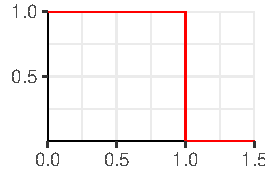
\includegraphics[scale=.4]{./img_ventanas/ventana_bartlett.pdf}\\
\rowcolor{gris}
Fejer &
$\displaystyle 
1-\abso{u}
$
& 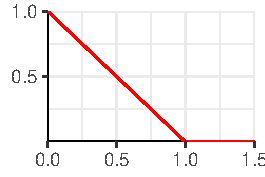
\includegraphics[scale=.4]{./img_ventanas/ventana_fejer.pdf} \\
Daniell &
$\displaystyle 
\frac{\SEN{\pi u}}{\pi u}
$
& 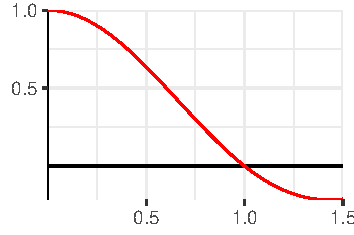
\includegraphics[scale=.4]{./img_ventanas/ventana_daniell.pdf} \\
\rowcolor{gris}
Bartlett-Priestley &
$\displaystyle 
\frac{3}{(\pi u)^{2}} \left[ \frac{\SEN{\pi u}}{\pi u} - \COS{\pi u} \right]
$
& 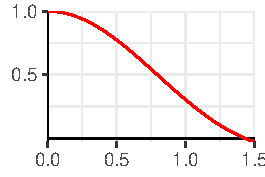
\includegraphics[scale=.4]{./img_ventanas/ventana_bartlet_priestley.pdf} \\
Cosenoidal &
$\displaystyle 
\COS{\pi u}
$
& 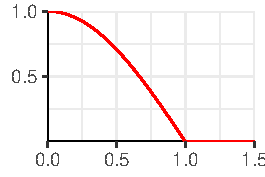
\includegraphics[scale=.4]{./img_ventanas/ventana_cosenoidal.pdf} \\
%\bottomrulec
\bottomrule
\end{tabular*}
\label{ventanas}
\end{SidewaysTable}

\begin{SidewaysTable}
\caption{Ejemplos de funciones ventana (función de transferencia)}
\centering
\begin{tabular}{lll}
\toprule
Nombre & $K(\theta)$ & Bosquejo \\
\midrule
Bartlett &
$\displaystyle 
\frac{1}{\pi} \frac{\SEN{\theta}}{\theta}
$
& 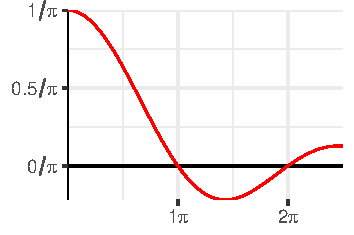
\includegraphics[scale=.4]{./img_ventanas/ventana_2_bartlett.pdf} \\
\rowcolor{gris}
Fejer &
$\displaystyle 
\frac{1}{2\pi} \left[ \frac{\SEN{\nicefrac{\theta}{2}}}{\nicefrac{\theta}{2}} \right]^{2}
$
& 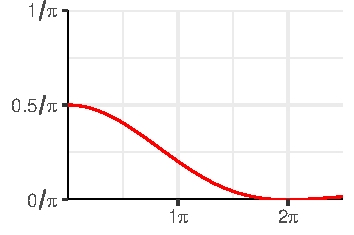
\includegraphics[scale=.4]{./img_ventanas/ventana_2_fejer.pdf} \\
Daniell &
$
\displaystyle 
\nicefrac{1}{2\pi} \text{, si } \abso{\theta}\leq \pi
$
& 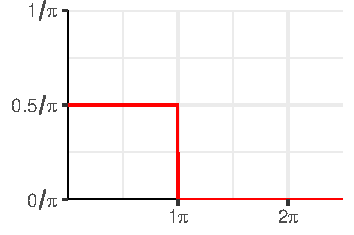
\includegraphics[scale=.4]{./img_ventanas/ventana_2_daniell.pdf} \\
\rowcolor{gris}
Bartlett-Priestley &
$\displaystyle 
\frac{3}{4 \pi} \left[ 1 - \left( \nicefrac{\theta}{\pi} \right) \right]
\text{, si } \abso{\theta}\leq \pi
$
& 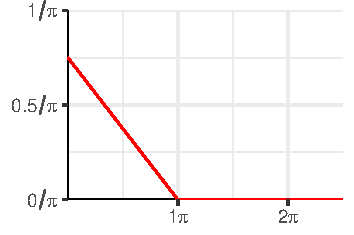
\includegraphics[scale=.4]{./img_ventanas/ventana_2_bartlet_priestley.pdf} \\
Cosenoidal &
$\displaystyle 
d
$
& 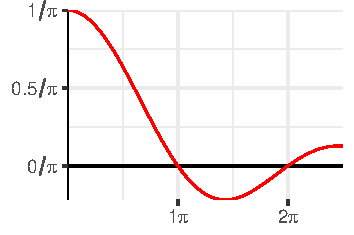
\includegraphics[scale=.4]{./img_ventanas/ventana_2_bartlett.pdf} \\
\bottomrule
\end{tabular}
\end{SidewaysTable}

%%%%%%%%%%%%%%%%%%%%%%%%%%%%%%%%%%%%%%%%%%%%%%%%%%%%%%%%%%%%%%%%%%%%%%%%%%%%%%%%%%%%%%%%%%%%%%%%%%%
%%%%%%%%%%%%%%%%%%%%%%%%%%%%%%%%%%%%%%%%%%%%%%%%%%%%%%%%%%%%%%%%%%%%%%%%%%%%%%%%%%%%%%%%%%%%%%%%%%%
%%%%%%%%%%%%%%%%%%%%%%%%%%%%%%%%%%%%%%%%%%%%%%%%%%%%%%%%%%%%%%%%%%%%%%%%%%%%%%%%%%%%%%%%%%%%%%%%%%%

%%%%%%%%%%%%%%%%%%%%%%%%%%%%%%%%%%%%%%%%%%%%%%%%%%%%%%%%%%%%%%%%%%%%%%%%%%%%%%%%%%%%%%%%%%%%%%%%%%%
%%%%%%%%%%%%%%%%%%%%%%%%%%%%%%%%%%%%%%%%%%%%%%%%%%%%%%%%%%%%%%%%%%%%%%%%%%%%%%%%%%%%%%%%%%%%%%%%%%%
%%%%%%%%%%%%%%%%%%%%%%%%%%%%%%%%%%%%%%%%%%%%%%%%%%%%%%%%%%%%%%%%%%%%%%%%%%%%%%%%%%%%%%%%%%%%%%%%%%%

\chapter{Espectro evolutivo}

En esta sección se introduce el \textit{espectro evolutivo}, una generalización del espectro de 
potencias para procesos no-estacionarios cuya estructura cambia lentamente en el tiempo.
%
Esta definición en particular fue presentada por Maurice Priestley en 1965 \cite{Priestley65}; la
información del presente capítulo puede revisarse con mayor detalle en su libro \textit{"Spectral
Analysis and Time Series"} \cite{Priestley81}, particularmente en el capítulo 11.

%Las secciones \ref{sec:frecuencias2}, ..., pueden verse como preliminares de este capítulo y pueden
%omitirse en una primera lectura, pues lidian con detalles sobre diferentes posibilidades para 
%generalización el espectro.

Es importante mencionar que la sección \ref{sec:espectro} representa la parte central de este
capítulo, describiendo un objeto matemático bien definido que lidia con un problema que roza la 
vaguedad; es por ello que viene acompañado de una discusión que podría ser omitida dentro del 
contexto global del trabajo, pero que tiene repercusiones importantes en el uso práctico del 
espectro evolutivo.
%
Por ejemplo, en la sección \ref{sec:estimacion} se discute sobre las condiciones bajo las cuales es 
\textit{posible} estimar el espectro evolutivo del proceso, mientras que la sección 
\ref{sec:doble_ventana} parte de tales condiciones para describir cómo efectuar la estimación.

Finalmente, en la sección \ref{sec:psr} se describe una aplicación aparentemente menor del espectro 
evolutivo, pero que constituye una parte central en el presente trabajo: la detección de 
estacionariedad débil a partir del espectro evolutivo.

%%%%%%%%%%%%%%%%%%%%%%%%%%%%%%%%%%%%%%%%%%%%%%%%%%%%%%%%%%%%%%%%%%%%%%%%%%%%%%%%%%%%%%%%%%%%%%%%%%%
%%%%%%%%%%%%%%%%%%%%%%%%%%%%%%%%%%%%%%%%%%%%%%%%%%%%%%%%%%%%%%%%%%%%%%%%%%%%%%%%%%%%%%%%%%%%%%%%%%%

\section{Definición del espectro evolutivo}
\label{sec:espectro}

Considérese un proceso estocástico a tiempo continuo \xtin{\R} que, por simplicidad, tiene media 
cero y varianza finita en todo momento, es decir
\begin{equation*}
\E{X(t)} = 0 \text{  ,  } \Var{X^{2}(t)} < \infty
\end{equation*}

Se define el \textit{núcleo de covarianza} para el proceso como
\begin{equation}
R(s,t) := \E{\overline{X(t)}X(s)}
\end{equation}

Conviene recordar el caso de un proceso estacionario, en el cual el núcleo de covarianza $R(t,s)$ 
puede verse como función de la variable $\abso{t-s}$, y en virtud del teorema de Winer-Khintchine 
acepta una representación de la forma
%
\begin{equation}
R(s,t) = \intR e^{i \omega (t-s)} dH(\omega)
\label{s6:kernel}
\end{equation}
%
donde $H$ es el espectro integrado del proceso y tiene las propiedades de una función de 
distribución sobre $\R$.
%
Como consecuencia, \xtin{\R} admite una representación de la forma
\begin{equation}
X(t) = \intR e^{i\omega t} dZ(\omega)
\end{equation}
%
donde $Z$ es un proceso estocástico que satisface
\begin{equation}
\Cov{dZ(\omega_1),dZ(\omega_2)} = 
\begin{cases}
dH(\omega_1) &, \text{si } \omega_1 = \omega_2 \\
0 &, \text{otro caso}
\end{cases}
\end{equation}

En general, se espera tener una generalización que conserve las propiedades anteriores. Con vista
a la ecuación \ref{s6:kernel}, puede restringirse la atención a procesos no-estacionarios que
acepten una representación de la forma
\begin{equation}
R(s,t) = \intR \overline{\phi(\omega;s)}\phi(\omega;t) d\mu(\omega)
\label{s6:erre}
\end{equation}
%
Para alguna medida $\mu$ definida en $\R$ y alguna familia de funciones 
$\ef = \left\{ \phi: \R \times \mathcal{T} \rightarrow \C \right\}$; debido a la interpretación que 
se le va a dar a este tipo de funciones, la variable $t\in \ef$ será referida como un índice.
%
Una condición a satisfacer es que $\Var{X^{2}(t)} = R(t,t) < \infty$, para lo cual cada 
$\phi \in \ef$ debe ser cuadrado integrable con respecto a $\mu$, es decir
\begin{equation}
\intR \phi^{2}(\omega;t) d\mu(\omega) < \infty
\end{equation}

Se puede demostrar t(4.11.12) que bajo estas condiciones el proceso \xt acepta una representación de la forma 
\begin{equation}
X(t) = \intR \phi(\omega;t) dZ(\omega)
\label{s6:representacion}
\end{equation}
donde el proceso $Z$ satisface que
\begin{equation}
\Cov{dZ(\omega_1),dZ(\omega_2)} = 
\begin{cases}
\mu(\omega_1) &, \text{si } \omega_1 = \omega_2 \\
0 &, \text{otro caso}
\end{cases}
\end{equation}


Se puede demostrar p(parzen 1959) que si un proceso admite una representación de la forma \ref{s6:representacion} para alguna familia de funciones $\ef$, entonces tiene admite múltiples
representaciones usando diferentes familias de funciones.
%
%Para poder dar a estas representaciones la interpretación de espectro, conviene usar una familia de
%funciones que conserven algunas propiedades de los senos y cosenos.
%

Para dar a estas representaciones la interpretación de espectro, conviene usar una familia de funciones que conserve algunas propiedades de los senos y cosenos; por ejemplo, las funciones oscilatorias

\begin{definicion}
Una función $\phi: \R \rightarrow \C$ se dice \textbf{oscilatoria} si admite una representación de la forma
\begin{equation}
\phi(t) = A(t) e^{i \omega t} 
\end{equation}
donde $A$ es de la forma
\begin{equation}
A(t) = \intR e^{i \omega t} dK(\omega)
\end{equation}
y donde $\abso{dK(\omega)}$ tiene un único máximo global en $\omega = 0$
\label{oscilatorio}
\end{definicion}

Si una función $\phi$ es oscilatoria como en la definición \ref{oscilatorio}, entonces puede entenderse como una función senoidal \textit{modulada} por una función $A$; no se permite que la función $A$ sea predominantemente periódica.

Como se mencionó, las expresiones \ref{s6:erre} y \ref{s6:representacion} pueden ser interpretadas como espectro si se usa una familia $\ef$ de funciones oscilatorias.

\begin{align}
R(s,t) &= \intR \overline{A(\omega; s)} A(\omega; t) e^{i\omega (t-s)} d\mu(\omega) \\
X(t) &= \intR A(\omega; t) e^{i \omega t} dZ(\omega)
\end{align}


\begin{definicion}
Sea \xt un proceso oscilatorio y $\ef$ una familia de funciones oscilatorias de la forma
$\phi(\omega;t) = A(\omega;t) e^{i \omega t}$. 
Sea $\mu$ tal que ...
Se define al \textbf{espectro evolutivo} del proceso respecto a la familia $\ef$ como
\begin{equation}
dH(t,\omega) := \abso{A(\omega;t)}^{2} d\mu(\omega)
\end{equation}
\label{def:oscilatorio}
\end{definicion}

%%%%%%%%%%%%%%%%%%%%%%%%%%%%%%%%%%%%%%%%%%%%%%%%%%%%%%%%%%%%%%%%%%%%%%%%%%%%%%%%%%%%%%%%%%%%%%%%%%%
%%%%%%%%%%%%%%%%%%%%%%%%%%%%%%%%%%%%%%%%%%%%%%%%%%%%%%%%%%%%%%%%%%%%%%%%%%%%%%%%%%%%%%%%%%%%%%%%%%%

\section{Estimación del espectro evolutivo}
\label{sec:estimacion}

En el capítulo anterior se mostró un estimador consistente para el espectro de potencias de un proceso estacionario; dicho estimador usaba la transformada de Fourier discreta, \textit{suavizada} por un filtro lineal (también referido como función ventana).
%
El objetivo de esta sección es aclarar algunos teoremas que permitan usar una técnica similar, la cual requiere imponer algunas condiciones más fuertes que ser oscilatorios.

\subsection{Filtros lineales}

Sea \xt un proceso oscilatorio, no necesariamente estacionario, y sea $g\in \lldos$; se construye al proceso $\{Y(t)\}_{t\in \mathcal{T}}$ como\footnote{En el texto de Priestley se considera un filtro de la forma $Y(t) = \intR g(u) X(t-u) e^{-i \omega_0 (t-u)} du$ para algún $\omega_0$ constante. 
Por simplicidad se considera únicamente el caso $\omega_0=0$}
\begin{equation}
Y(t) = \intR g(u) X(t-u) du
\end{equation}

Entonces puede escribirse 
\begin{equation}
Y(t) = \intR \Gamma_t(\omega) e^{i \omega t} dZ(\omega) 
\label{se6:filtrado}
\end{equation}
donde $\Gamma_\bullet$ es la \textbf{función de transferencia generalizada} para $g$ con respecto a la familia $\ef$, y que es definida como
\begin{equation}
\Gamma_t (\omega) := \intR g(u) A(\omega; t-u) e^{i \omega u} du
\label{se6:trans_general}
\end{equation}

%En general no puede garantizarse que la expresión en \ref{se6:filtrado} satisfaga las propiedades de un espectro evolutivo; si se escribe
%\begin{equation*}
%\Gamma_t(\omega) = \intR e^{i \omega t} dK(\omega)
%\end{equation*}
%no siempre se cumple que $\abso{dK}$ tiene un único máximo global en 0.

Un caso particular muy interesante ocurre cuando $A$, como función de $\omega$, varía lentamente en comparación de $g$, la cual decae rápidamente a 0; en tal caso podría decirse que $\Gamma_\bullet \approx \Gamma$


\begin{definicion}
Una familia de funciones $\ef$ se dice \textbf{semi-estacionaria} si, para todo $\omega \in \R$, se cumple que
\begin{equation}
\intR \abso{\omega} \abso{dK(\omega)} < \infty
\end{equation}
En cuyo caso se define su \textbf{ancho característico}
\begin{equation}
B_\ef := \left[ \sup_\omega \intR \abso{\omega} \abso{dK(\omega)} \right]^{-1}
\end{equation}
\end{definicion}

\begin{definicion}
Un proceso \xt se dice \textbf{semi-estacionario} si admite una representación de la forma \ref{s6:representacion} para alguna familia semi-estacionaria
\end{definicion}

%\begin{definicion}
%Sea \xt un proceso semi-estacioario, y sea $\mathcal{C}$ la clase de las familias semi-estacionarias con las cuales el proceso admite una representación de la forma [?].
%Se define el \textbf{ancho de banda característico} de \xt como 
%\begin{equation}
%B_X := \sup_{\ef \in \mathcal{C}} B_\ef
%\end{equation}
%\end{definicion}

\begin{definicion}
Se dice que una función $u$ es 
\textbf{pseudo-$\boldsymbol{\delta}$ de orden $\boldsymbol{\varepsilon}$} con respecto a la función $v$ si, para cualquier $k$ existe un $\varepsilon << 1$ tal que 
\begin{equation}
\abso{\intR u(x) v(x+k) dx  -  v(k)\intR u(x)} < \varepsilon
\end{equation}
\end{definicion}


De manera similar, se define el \textbf{ancho de banda} para $g$ como 
\begin{equation}
B_g := \intR \abso{u} \abso{g(u)} du
\end{equation}

Supóngase que $g$ está normalizada de modo que
\begin{equation}
2 \pi \intR \abso{g(u)}^{2} du = \intR \abso{\Gamma(\omega)} d\omega = 1
\label{s6:norm_g}
\end{equation}
con $\Gamma$ la función de respuesta para $g$.

\begin{teorema}
Sea $\ef$ una familia semi-estacionaria con ancho de banda característico $B_\ef$, y sea $g$ una función normalizada como en \ref{s6:norm_g} y cuyo ancho de banda es $B_g$. Entonces, para cualesquiera $t, \omega \in \R$ se cumple que $e^{i \omega t} dK(\omega)$ es una función pseudo-$\delta$ de orden $\nicefrac{B_g}{B_\ef}$ con respecto a $g$
\label{teo:s6:lema}
\end{teorema}
\begin{proof}
Suponiendo que $\Gamma$ sea una vez derivable, su expansión de Taylor alrededor de $k$ es
\begin{equation*}
\intR e^{i\theta t} \Gamma(\theta + k) dK(\omega)
= \Gamma(k) \intR e^{i \theta t} dK(\omega) + 
\intR e^{i \theta t} \theta \Gamma\prima(k + \nu) dK(\omega)
\end{equation*}
para algún $\nu \in (0,\theta)$. Respecto al segundo sumando, puede observarse que
\begin{align*}
\intR e^{i \theta t} \theta \Gamma\prima(k + \nu) dK(\omega)
&\leq
\abso{ \intR e^{i \theta t} \theta \Gamma\prima(k + \nu) dK(\omega)} \\
&\leq
\intR \abso{ \theta} \abso{ \Gamma\prima(k + \nu)} \abso{ dK(\omega)} \\
&\leq
\intR \abso{ \theta} \left[ \sup_\omega \abso{ \Gamma\prima(\omega)} \right] \abso{ dK(\omega)} \\
&\leq
\left[ \sup_\omega \abso{ \Gamma\prima(\omega)} \right]
\left[ \sup_\omega
\intR \abso{ \theta} \abso{ dK(\omega)} \right]
\end{align*}
Usando la conexión entre $g$ y $\Gamma$
\begin{align*}
\Gamma\prima(\omega) 
&= \frac{d}{d\omega} \left( \intR e^{i \omega u} g(u) du \right) \\
&= \intR \left( \frac{d}{d\omega} e^{i \omega u} g(u) \right) du \\
&= i \intR u e^{i \omega u} g(u) du \\
\end{align*}
Luego entonces
\begin{align*}
\intR e^{i \theta t} \theta \Gamma\prima(k + \nu) dK(\omega)
&\leq
\left[ \sup_\omega \abso{ \Gamma\prima(\omega)} \right] 
\left[ \sup_\omega
\intR \abso{ \theta} \abso{ dK(\omega)} \right] \\
&\leq 
\left[ \sup_\omega \abso{ \intR i u e^{i \omega u} g(u) du } \right] 
B_\ef^{-1} \\
&\leq 
B_\ef^{-1}
\left[ \sup_\omega \intR \abso{ u } \abso{ g(u)} du \right] \\
&\leq
B_\ef^{-1} B_g
\end{align*}
\end{proof}

Con el teorema anterior a la mano se puede declarar formalmente la idea de que $A$ varía más lentamente que $g$

\begin{teorema}
Sea $\ef$ una familia semi-estacionaria con ancho de banda característico $B_\ef$, sea $\varepsilon >0$ arbitrario, y sea $g$ un filtro normalizado como en \ref{s6:norm_g} y cuya función de transferencia generalizada con respecto a $\ef$ es $\Gamma_\bullet$. 
%
Si $g$ es elegida de tal modo que $\nicefrac{B_g}{B_\ef} < \varepsilon$, entonces para cualesquiera $t, \omega$ se cumple que
\begin{equation}
\abso{\Gamma_t(\omega)- A(\omega; t)\Gamma(\omega)} < \varepsilon
\end{equation}
\label{teo:aprox_gamma} 
\end{teorema}

\begin{proof}
Por la mera definición de $\Gamma_\bullet$ (expresión \ref{se6:trans_general}) se sabe que
\begin{equation*}
\Gamma_t (\omega) = \intR g(u) A(\omega; t-u) e^{i \omega u} du
\end{equation*}
Si se sustituye a $A$ en términos de $dK$ (ver definición \ref{def:oscilatorio})
\begin{align*}
\Gamma_t (\omega) &= \intR g(u) A(\omega; t-u) e^{i \omega u} du \\
&= 
\intR g(u) \left[ \intR e^{i \theta (t-u)} dK(\theta) \right] e^{i \omega u} du \\
&=
\intR \intR g(u) e^{i \theta t} e^{i (\omega- \theta) u} dK(\theta) du \\
&=
\intR e^{i \theta t} \left[ \intR g(u) e^{i (\omega- \theta) u} du \right] dK(\theta) \\
&=
\intR e^{i \theta t} \Gamma(\omega - \theta) dK(\theta) \\
\end{align*}
Usando el lema \ref{teo:s6:lema} junto al hecho que $\nicefrac{B_g}{B_\ef} < \varepsilon$, se puede escribir que
\begin{align*}
\varepsilon 
&> 
\abso{\intR e^{i \theta t} \Gamma(\omega - \theta) dK(\theta) - 
\Gamma(\omega) \intR e^{i \theta t} dK(\theta) } \\
&=
\abso{\Gamma_t (\omega) - 
\Gamma(\omega) \intR e^{i \theta t} dK(\theta) } \\
&=
\abso{\Gamma_t (\omega) - 
\Gamma(\omega) A(\omega; t) }
\end{align*}
En el último renglón se ha reemplazado nuevamente a $A$ en términos de $dK	$
\end{proof}

\begin{teorema}
Sea \xt un proceso semi-estacionario con ancho de banda característico $B_X$, sea $g$ un filtro normalizado como en \ref{s6:norm_g} y cuyo ancho de banda es $B_g$ y cuya función de respuesta es $\Gamma$. 
%
Sea $\{Y(t)\}_{t\in \mathcal{T}}$ un proceso definido como \ref{se6:filtrado}.

Sea $\efstar$ una familia semi-estacionaria cuyo ancho de banda característico es $B_X$ o es muy parecido a $B_X$ (lo cual es posible por cómo se definió $B_X$).
Se cumple que
\begin{equation}
\E{\abso{Y(t)}^{2}} = \intR \abso{\Gamma(\omega)}^{2} dH^{*}(\omega; t) + \orden{\epsilon}
\end{equation}
donde $H^{*}$ es el espectro integrado respecto a la familia $\efstar$ y $\orden{\epsilon}$ es un término que puede hacerse arbitrariamente pequeño si $B_g$ es suficientemente pequeño respecto a $B_X$
\label{teo:aprox_orden}
\end{teorema}

\begin{proof}
Usando la expresión \ref{se6:filtrado} para este caso particular, puede escribirse
\begin{equation}
Y(t) = \intR \Gamma_t^{*} (\omega; t) A^{*}(\omega; t) e^{i \omega t} dZ^{*}(\omega)
\end{equation}
donde $\omega_\bullet^{*}$, $A^{*}$ y $Z^{*}$ están definidos respecto a la familia $\efstar$.
Nótese que, debido a que los $dZ$'s son ortogonales
\begin{align*}
\E{\abso{Y(t)}^{2}} 
&= 
\E{
\overline{\intR \Gamma_t^{*} (\omega; t) e^{i \omega t} dZ^{*}(\omega)}
\intR \Gamma_t^{*} (\omega; t) e^{i \omega t} dZ^{*}(\omega) }\\
&= ... \\
&= \intR \abso{\Gamma_t^{*} (\omega; t)}^{2} d\mu^{*}(\omega)
\end{align*}

Si se elige a $g$ de modo que $\frac{B_g}{B_X} < \varepsilon$, en virtud del teorema \ref{teo:aprox_gamma} puede escribirse
\begin{equation}
\Gamma_t^{*}(\omega; t) = A^{*}(\omega; t) \Gamma(\omega) + R(\omega; t)
\end{equation}
con $\abso{R(\omega,t)} < \varepsilon$. Luego entonces
\begin{align*}
\E{\abso{Y(t)}^{2}} 
&= 
\intR \abso{\Gamma_t^{*} (\omega; t)}^{2} d\mu^{*}(\omega) \\
&= 
\intR \abso{A^{*}(\omega; t) \Gamma(\omega) + R(\omega; t)}^{2} d\mu^{*}(\omega) \\
&= 
\intR \abso{A^{*}(\omega; t) \Gamma(\omega)}^{2} d\mu^{*}(\omega) +\\
&\pheq
\intR \overline{A^{*}(\omega; t) \Gamma(\omega)} R(\omega; t) d\mu^{*}(\omega) +\\
&\pheq
\intR A^{*}(\omega; t) \Gamma(\omega) \overline{ R(\omega; t)} d\mu^{*}(\omega) +\\
&\pheq
\intR \abso{R(\omega; t)}^{2} d\mu^{*}(\omega) 
\end{align*}

El cuarto sumando satisface claramente que
\begin{equation}
\intR \abso{R(\omega; t)}^{2} d\mu^{*}(\omega)  < \varepsilon^{2} \intR d\mu^{*}(\omega) 
= \orden{\varepsilon^{2}}
\end{equation}

Respecto al segundo sumando, nótese que 
\begin{align*}
\intR \overline{A^{*}(\omega; t) \Gamma(\omega)} R(\omega; t) d\mu^{*}(\omega)
&< \intR \abso{A^{*}(\omega; t)} \abso{ \Gamma(\omega)} \abso{R(\omega; t)} d\mu^{*}(\omega) \\
&< \varepsilon \intR \abso{A^{*}(\omega; t)}\abso{ \Gamma(\omega)} d\mu^{*}(\omega)
\end{align*}
Una cota similar puede hallarse para el tercer sumando.
Falta demostrar que la cota permanece finita cuando $B_g \rightarrow 0$, lo cual debería lograrse definicendo el conjunto
\begin{equation}
\Omega = \left\{ \omega \in \R | \abso{\Gamma(\omega)} \abso{A^{*}(\omega; t)} \leq 1 \right\} 
\end{equation}
y luego, claramente
\begin{equation}
\intR \abso{A^{*}(\omega; t)}\abso{ \Gamma(\omega)} d\mu^{*}(\omega) = 
\int_\Omega \mu^{*}(\omega) + 
\int_{\Omega^{C}} \abso{A^{*}(\omega; t)}\abso{ \Gamma(\omega)} d\mu^{*}(\omega)
\end{equation}
el primer sumando es clarametne finito y no depende de $g$, mientras que el segundo debería ser finito [?] ya que $\Gamma$ está normalizada.
\end{proof}

%%%%%%%%%%%%%%%%%%%%%%%%%%%%%%%%%%%%%%%%%%%%%%%%%%%%%%%%%%%%%%%%%%%%%%%%%%%%%%%%%%%%%%%%%%%%%%%%%%%
%%%%%%%%%%%%%%%%%%%%%%%%%%%%%%%%%%%%%%%%%%%%%%%%%%%%%%%%%%%%%%%%%%%%%%%%%%%%%%%%%%%%%%%%%%%%%%%%%%%

\section{Estimador de doble ventana}
\label{sec:doble_ventana}

Para esta sección se considera un proceso a tiempo continuo \xtin{\R} y una muestra del mismo de longitud $T$ (o equivalentemente un proceso \xtin{[0,T]}), suficientemente larga. El objetivo en esta sección es construir un estimador para el espectro evolutivo $dH(\omega; t)$.
%
Por simplicidad, se supondrá que la medida $\mu$ es absolutamente continua respecto a la medida de Lebesgue, y entonces puede escribirse
\begin{equation}
h(\omega,t) := dH(\omega; t)
\end{equation}

Para efectuar la estimación del espectro se hará uso del teorema \ref{teo:aprox_gamma}, para lo cual se necesita un filtro $g$ normalizado según \ref{s6:norm_g} y cuyo anho de banda, $B_g$, satisface
\begin{equation}
B_g << B_X << T
\label{s6:anchos_banda}
\end{equation}

Se construye entonces a $U$, una versión filtrada de $X$ usando a $g$
\begin{equation}
U(t) = \int_{t-T}^{t} g(u) X(t-u) du
\end{equation}

Bajo la condición \ref{s6:anchos_banda}, la integral que define a $U$ puede extenderse a todo $\R$ sin cambiar mucho su valor (excepto cerca de 0 y $T$), e incluso se llega a ser exacta si $g$ es 0 fuera de un intervalo pequeño alrededor de 0. Entonces, en virtud del teorema \ref{teo:aprox_orden}
aplica de manera aproximada, y entonces se cumple que
\begin{equation}
\E{\abso{U(\omega; t)}^{2}} = \intR \abso{\Gamma(\omega)}^{2} h(\omega, t)d\omega + \orden{\nicefrac{B_g}{B_X}}
\end{equation}


\begin{proposicion}
Dadas las condiciones, y si \xt es un proceso normal cuyo que admite un espectro evolutivo uniformemente continuo, se tiene que
\begin{equation}
\Var{\abso{U(\omega;t)}^{2}} \approx \left[ \intR \abso{\Gamma(\omega)}^{2} h(\omega, t)d\omega \right]^{2}
\end{equation}
\end{proposicion}

La demostración al teorema anterior puede ahllarse en el artículo de Maurice Priestley \textit{Design Relations for Non-Stationary Processes} \cite{Priestley66}, sección 3.

%\begin{proof}
%En general, puede escribirse para $t,s \in \mathcal{T}$, $\omega, \lambda \in \R$
%\begin{align*}
%\Cov{\abso{U(\omega;t)}^{2},\abso{U(\lambda;s)}^{2}} &=
%\E{\abso{U(\omega;t)}^{2},\abso{U(\lambda;s)}^{2}} \\
%&=
%\int \int \int \int_{R^{4}} g(u) g(v) g(w) g(z) e^{i u \omega} e^{i v \omega} e^{i w \lambda} e^{i z \lambda} \\
%&\pheq \times
%\E{{X(t-u)} {X(t-v)} {X(s-w)} {X(s-z)}}
%du dv dw dz 
%\end{align*}
%Si \xt es normal, entonces
%\begin{align*}
%\E{X(t-u) {X(t-v)} {X(t-w)} X(t-z)} &=
%R(t-u,t-v)R(s-w,s-z) \\
%&\pheq + R(t-u,s-z)R(t-v,s-w) \\
%&\pheq + R(t-u,s-w)R(t-v,s-z)
%\end{align*}
%donde
%\begin{equation}
%R(p,q) = \intR e^{i \omega (p-q)} A(\omega; p)\overline{A(\omega; q)} d\mu(\omega) 
%\end{equation}
%Así entonces, puede escribirse
%\begin{align*}
%\Cov{\abso{U(\omega;t)}^{2},\abso{U(\lambda;s)}^{2}} &=
%\E{\abso{U(\omega, t)}^{2}} \E{\abso{U(\lambda, s)}^{2}} + S_1 + S_2
%\end{align*}
%donde
%\begin{align*}
%S_1 &= 
%\int \int \int \int_{\R^{4}} g(u) g(v) g(w) g(z) e^{i u \omega} e^{i v \omega} e^{i w \lambda} e^{i z \lambda} \\
%&\pheq \times \left( 
%\int \int_{\R^{2}} 
%\left[ 
%e^{-i \theta (s-z-t+u)} A(\theta; t-u) \overline{A(\theta; s-z)} 
%\right] 
%\right. \\
%&\pheq 
%\left. \vphantom{\int}
%\left[ e^{-i \phi (s-w-t+u)} A(\phi; t-v) \overline{A(\theta; s-w)} \right] d\theta d\phi
%\right) du dv dw dz
%\end{align*}
%Puede escribirse
%\begin{align*}
%S_1 &= \int \int_{\R^{2}} \Gamma(\theta+ \omega; t, \theta) \overline{\Gamma(\phi + \omega; t, \phi)}
% \Gamma(\phi+ \lambda; s, \phi) \overline{\Gamma(\theta + \lambda; s, \theta)} \\
% &\pheq \times
% \left[
% A(\theta; t) \overline{A(\phi; t)} A(\phi; s) \overline{A(\theta; t)}
% \right] d\theta d\phi
%\end{align*}
%Usando el teorema [?], si $B_g << B_X$ entonces $\Gamma(\bullet; t, \lambda) \approx \Gamma(\bullet)$, luego
%\begin{align*}
%S_1 &\approx \left[ e^{-i \theta (s-t) } A(\theta; t) \overline{A(\theta; s)} \Gamma(\theta + \omega) \Gamma(\theta + \lambda) d\theta\left] \\
%\phantom{\approx} \times
%\left[ e^{-i \phi (s-t) } A(\theta; t) \overline{A(\phi; s)} \Gamma(\phi + \omega) \Gamma(\phi + \lambda) d\phi\left] \\
%\end{align*}
%\end{proof}

Un resultado que es muy análogo a la estimación del espectro en el caso de estacionariedad.
%
Siguiendo con la analogía, este problema es resuelto al usar un filtro $w_\tau$ que satisfaga las siguientes propiedades
\begin{itemize}
\item $w_\tau(t) \geq 0$ para cualesquiera $t$, $\tau$
\item $w_\tau(t) \rightarrow 0$ cuando $\abso{t} \rightarrow \infty$, para todo $\tau$
\item $\displaystyle \intR w_\tau(t) dt = 1$ para todo $\tau$
\item $\displaystyle \intR \left( w_\tau(t) \right)^{2} dt < \infty$ para todo $\tau$
\item $\exists C \in \R$ tal que  
$\displaystyle \lim_{\tau\rightarrow\infty} \tau \intR \abso{ W_{\tau}(\lambda) }^{2} d\lambda = C$
\end{itemize}
donde $W_\tau = \intR e^{-i \lambda t} w_\tau(t) d\lambda$. Se define el segundo estimador
\begin{equation}
V(t) = \int_{T-t}^{t} w_\tau (u) \abso{U(t-u)}^{2} du
\label{estimador_doble_ventana}
\end{equation}

El supuesto sobre que $g$ decaiga lejos de 0, aplicado ahora a $w_\tau$, permite reemplazar el intervalo de integración que define a $V$ por $\R$. 

De manera sencilla puede verse que
\begin{align*}
\E{V(t)} &= 
\E{\intR w_\tau (u) \abso{U(t-u)}^{2} du} \\
&= 
\int_{T-t}^{t} w_\tau (u) \E{\abso{U(t-u)}^{2}} du \\
&=
\intR w_\tau (u) \left[
\intR \abso{\Gamma(\omega)}^{2} h(\omega, t-u)d\omega + \orden{\nicefrac{B_g}{B_X}} \right] du \\
&=
\intR \intR w_\tau (u) \abso{\Gamma(\omega)}^{2} h(\omega, t-u)d\omega du +
\orden{\nicefrac{B_g}{B_X}} \intR w_\tau (u) du \\
&=
\intR \abso{\Gamma(\omega)}^{2} \left[ \intR w_\tau (u) h(\omega, t-u) du \right] d\omega du +
\orden{\nicefrac{B_g}{B_X}} \intR w_\tau (u) du \\
&=
\intR \abso{\Gamma(\omega)}^{2} \overline{h}(\omega,t) d\omega du +
\orden{\nicefrac{B_g}{B_X}} \\
\end{align*}
donde
\begin{equation}
\overline{h}(\omega,t) = \intR w_\tau (u) h(\omega, t-u) du
\end{equation}

Es demostrado en Priestley [1966?] que
\begin{equation}
\Var{V(t)} \approx \widetilde{h}^{2}(\omega_0,t) \left[ \intR \abso{W_\tau(\omega)}^{2} d\omega \right] \left[ \intR \abso{\Gamma(\omega)}^{4} \right] (1+\delta(0,\omega_0))
\end{equation}
donde
\begin{equation}
\widetilde{h}^{2} = \frac{\intR h^{2}(\omega_0,t) \left(w_\tau(u)\right)^{2}}{\intR \left(w_\tau(u)\right) du}
\end{equation}

Aún más, si se usa la propiedad de en el límite de $\tau W_\tau$ se puede escribir
\begin{equation}
\Var{V(t)} \approx 
\widetilde{h}^{2}(\omega_0,t) \frac{C}{\tau} \left[ \intR \abso{\Gamma(\omega)}^{4} \right] (1+\delta(0,\omega_0))
\end{equation}

Una aproximación muy similar 
puede hacerse respecto al segundo término, de modo que $\widetilde{h}\approx h$ y 
$\overline{h}^{2}\approx h^{2}$.
Tales aproximaciones serán mejores en tanto las ventanas $w_{\tau}$ y $W_{\tau}$ sean más 
cercanas a funciones tipo \dirac.
Dicho esto, se pueden hacer las siguientes aproximaciones, un poco más arriesgadas:
\begin{itemize}
\item $\displaystyle \E{\est{h}(t,\omega)} \approx h(t,\omega)$
\item $\displaystyle \Var{\est{h}(t,\omega)} \approx 
\frac{C}{\tau} h^{2}(t,\omega) \intR \abso{\Gamma_\kappa (\theta)}^{4} d\theta$
\end{itemize}

%%%%%%%%%%%%%%%%%%%%%%%%%%%%%%%%%%%%%%%%%%%%%%%%%%%%%%%%%%%%%%%%%%%%%%%%%%%%%%%%%%%%%%%%%%%%%%%%%%%
%%%%%%%%%%%%%%%%%%%%%%%%%%%%%%%%%%%%%%%%%%%%%%%%%%%%%%%%%%%%%%%%%%%%%%%%%%%%%%%%%%%%%%%%%%%%%%%%%%%

\section{Prueba de Priestley-Subba Rao}
\label{sec:psr}

La prueba de estacionariedad propuesta por Priestley y Subba Rao \cite{Priestley69} consiste en 
probar la hipótesis de que el espectro evolutivo efectivamente cambia en el tiempo. 
%
El proceso consiste en \textit{calcular} el logaritmo del espectro evolutivo para algunos tiempos y 
frecuencias puntuales, para lo cual se usa el estimador de doble ventana, y posteriormente usar un
análisis ANOVA para verificar si dichas cantidades tienen el mismo valor esperado --recordando que
el estimador de doble ventana es asintóticamente consistente.

Sea \xt un proceso semi-estacionario y sea \xtd un conjunto de observacion, cuya frecuencia de 
muestreo es $\Delta_t=1$ por simplicidad.
%
Usando estos datos se construye el estimador de doble ventana, $\widehat{h}$; para ello se eligen 
como parámetros las funciones $g_\kappa$ y $w_\tau$, que dependen a su vez de los parámetros 
$\kappa$ y $\tau$, y por consecuencia a sus respectivas tr. de Fourier $\Gamma_\kappa$ y $W_\tau$.
%
Bajo las condiciones descritas en la sección anterior, se satisface que
%
\begin{align*}
\E{\widehat{h}(t,\omega)} &\approx h(t,\omega) \\
\Var{\widehat{h}(t,\omega)} &\approx 
\frac{C}{N} h^{2}(t,\omega) \intR \abso{\Gamma^{4}(\theta)} d\theta
\end{align*}
%
donde $\displaystyle C = \lim_{T\rightarrow \infty} T \intR \abso{W_T(\lambda)} d\lambda$.
%
Como es habitual en el estudio del espectro de potencias, se propone la cantidad 
\begin{equation}
Y(t,\omega) = \log\left(\widehat{h}(t,\omega)\right)
\end{equation}
que, por ser $\log$ una función inversible y derivable, cumple que
%
\begin{align*}
\E{Y(t,\omega)} &\approx \log\left(h(t,\omega)\right) \\
\Var{Y(t,\omega)} &\approx 
\frac{C}{T} \intR \abso{\Gamma_\kappa(\theta)}^{4} d\theta \\
\end{align*}

Cabe destacar que la varianza de $Y$ no es independiente de $h$ en el sentido formal, sino que 
sólo es \textit{aproximadamente independiente} pues depende en mayor medida de la forma de 
$\widehat{h}$ que del mismo $h$.
%
Esto era de esperarse, ya que el estimador de doble ventana fue diseñado para exagerar el 
\textit{peso} de la información local. 
%
En otra dirección, la independencia aproximada sugiere que $Y$ puede escribirse como

\begin{equation}
Y(t,\omega) = \log\left(h(t,\omega) \right) + \varepsilon(t,\omega)
\label{ye}
\end{equation}
%la cual \textit{hereda} las características
%\begin{align*}
%\E{\varepsilon(t,\omega)} &\approx 0 \\
%\Var{\varepsilon(t,\omega)} 
%&\approx \frac{C}{T} \intR \abso{\Gamma_\kappa(\theta)}^{4} d\theta
%\end{align*}

El que la varianza de $Y$ sea aproximadamente constante en todos los tiempos y frecuencias lo hace 
una excelente elección para verificar que el espectro evolutivo es constante en el tiempo.
%
Dos problemas respecto a la expresión \ref{ye} son (1) la covarianza de $\varepsilon$ entre
tiempos y frecuencias y (2) computacionalmente sólo es posible evaluar a $Y$ sobre una malla
de puntos en tiempo y frecuencia.

Sea una malla de puntos en el tiempo y las frecuencias, equiespaciado en el tiempo con distancia 
$\delta_t$ y en las frecuencias con distancia $\delta_\omega$.
%$\left\{ (t_i,\omega_j) \in \mathcal{T} \times [-\pi,\pi] | i = 1,\dots,I ; j=1,\dots,J \right\}$
Es demostrado en \cite{Priestley66} que si $\delta_\omega$ o $\delta_t$ son suficientemente grandes
como para que se cumpla alguna de las condiciones en \ref{separacion}, entonces los valores de $Y$
sobre la cuadrícula son aproximadamente no-correlacionados.

\begin{equation}
\left.
\begin{aligned}
\intR \abso{\Gamma_\kappa(\theta)}^{2}\abso{\Gamma_\kappa(\theta+\delta_\omega)}^{2} d\theta 
&\approx 0 \\
\frac{1}{\delta_t} \intR \abso{t} \abso{w_\tau (t)} dt &\approx 0
\end{aligned}
\right\rbrace
\Rightarrow
\Cov{Y(t,\omega),Y(t,\omega_0)} \approx 0
\label{separacion}
\end{equation}

Así entonces, sea
$\left\{ (t_i,\omega_j) \in \mathcal{T} \times [-\pi,\pi] | i = 1,\dots,I ; j=1,\dots,J \right\}$
la cuadrícula descrita, con $\delta_t= \abso{t_i - t_{i+1}}$ y 
$\delta_\omega = \abso{\omega_j-\omega_{j+1}}$. 
%
Se define el estimador
\begin{equation}
Y_{i,j} = \log\left(\widehat{h}(t_i,\omega_j)\right)
\end{equation}
%
el cual tiene las siguientes propiedades
%
\begin{align*}
Y_{i,j} &\approx \log\left(h(t_i,\omega_j)\right) + \varepsilon_{i,j} \\
\E{\varepsilon_{i,j}} &\approx 0 \\
\Var{\varepsilon_{i,j}} &\approx
\frac{C}{T} \intR \abso{\Gamma_\kappa(\theta)}^{4} d\theta \\
\Cov{\varepsilon_{i,j},\varepsilon_{i_0,j_0}} &\approx 0 
\Leftarrow (i,j)\neq (i_0,j_0)
\end{align*}

%Si el número de puntos es \textit{suficientemente grande}, entonces aproximadamente
%$\varepsilon_{i,j} \sim N(0,\sigma^{2})$.

Una vez definido un estimador adecuado para detectar la estacionariedad débil, conviene escribir
explícitamente las condiciones para tal detección.
%
La estacionariedad débil, en términos del espectro evolutivo $h$, puede expresarse como
%
\begin{equation*}
H_{E_1} : h(t_0,\omega_j) = h(t_1,\omega_j) = \cdots = h(t_I,\omega_j)
\text{ , para } j = 1, 2, \dots , J
\end{equation*}
%
condición que puede reescribirse\footnote{$H_{E_1}$ y $H_{E_2}$ son equivalentes en cuanto a la
decisión que producen} en términos de $Y$, en su versión discreta
%
\begin{equation*}
H_{E_2} : \E{Y_{0,j}} = \E{Y_{1,j}} = \cdots = \E{Y_{I,j}} \text{ , para } j = 1, 2, \dots , J
\end{equation*}
%
la cual, a su vez, puede reescribirse como
\begin{equation*}
H_{E_3} : \E{\varepsilon_{0,j}} = \E{\varepsilon_{1,j}} = \cdots =
\E{\varepsilon_{I,j}} \text{ , para } j = 1, 2, \dots , J
\end{equation*}

Sin embargo, la condición $H_{E_3}$ es una consecuencia directa de las propiedades de $Y$ si
$H_{E_2}$ es cierta; este \textit{juego} de equivalencias pierde consistencia si resulta que
$H_{E_3}$ fuera rechazada, lo cual implicaría en una contradicción.

El objetivo de la prueba puede fijarse en verificar efectivamente ocurre la contradicción
referida, en cuyo caso se podrá concluir que el proceso \textbf{no} es débilmente estacionario.
%
Con base a la forma de $H_{E_2}$, la prueba puede formularse en términos de un análisis ANOVA de dos
factores, el cual parte de un modelo general
%
\begin{equation*}
H_0 : Y_{i,j} = \mu + \alpha_i + \beta_j + \gamma_{i,j} + \varepsilon_{i,j}
\end{equation*}
%
donde $\varepsilon$ es como se definió anteriormente. 
%
Dentro del contexto, las cantidades involucradas pueden interpretarse como
\begin{description}
\item[$\mu$] Promedio de $h$ sobre tiempo y frecuencia
\item[$\alpha$] Efecto al variar el tiempo
\item[$\beta$] Efecto al variar la frecuencia
\item[$\gamma$] Efecto no lineal de tiempo y frecuencia (\textit{interacción})
\end{description}

La diferencia entre $\gamma$ y $\varepsilon$ consiste en que se conocen (por diseño) la media y 
varianza de $\varepsilon$, y se espera que siga una distribución normal si se cuentan con 
suficientes puntos; en contraparte, no se ha supuesto nada sobre $\gamma$.

Ahora bien, la hipótesis $H_{E_2}$ puede reescribirse para contrastarse contra $H_0$ como
%
\begin{equation*}
H_A : \hspace{1em} Y_{i,j} = \mu + \alpha_i + \varepsilon_{i,j}
\end{equation*}

Por simplicidad, conviene considerar un paso intermedio
\begin{equation*}
H_{\text{inter}} : Y_{i,j} = \mu + \alpha_i + \beta_j + \varepsilon_{i,j}
\end{equation*}

Como es usual con los ANOVA, se definen las sumas de cuadrados dentro de los grupos y entre los
grupos (cuadro \ref{cantidades_psr}), las cuales siguen distribuciones $\chi^{2}$.
%
Al probar $H_0$ contra $H_{\text{inter}}$ se usa el estadístico de prueba 
$\nicefrac{S_{I+R}}{\sigma^{2}}$, mientras que al probar $H_{\text{inter}}$ contra $H_A$ se usa
$\nicefrac{S_T}{\sigma^{2}} = 0$.

\begin{table}
\caption{Estadísticos involucrados en la prueba PSR}
\centering
\bordes{1.1}
\begin{tabular}{lll}
\toprule
Descripción & Estadístico & {Gr. de libertad} \\
\midrule
Efecto tiempo &
$S_T =J \sum_{i=1}^{I} \left( Y_{i,\bullet} - Y_{\bullet,\bullet} \right)^{2}$ 
& $I-1$ \\
Efecto frecuencia &
$S_F = I \sum_{j=1}^{J} \left( Y_{\bullet,j} - Y_{\bullet,\bullet} \right)^{2}$ 
& $J-1$ \\
Interacción &
$S_{I+R} = \sum_{i=1}^{I} \sum_{j=1}^{J} 
\left( Y_{i,j} - Y_{i,\bullet} - Y_{\bullet,j} + Y_{\bullet,\bullet} \right)^{2}$ 
& $(I-1)(J-1)$ \\
%\midrule
\rowcolor{gris}
Total &
$S_{0} = \sum_{i=1}^{I} \sum_{j=1}^{J} 
\left( Y_{i,j} - Y_{\bullet,\bullet} \right)^{2}$ 
& $IJ -1$ \\
\midrulec
Prom. tiempo &
$Y_{i,\bullet} = \frac{1}{J} \sum_{j=1}^{J} Y_{i,j}$ & \\
Prom. frecuencia &
$Y_{\bullet,j} = \frac{1}{I} \sum_{i=1}^{I} Y_{i,j}$ & \\
Prom. general &
$Y_{\bullet,\bullet} = \frac{1}{I J} \sum_{i=1}^{I} \sum_{j=1}^{J} Y_{i,j}$ & \\
\bottomrule
\end{tabular} \\
\label{cantidades_psr}
\end{table}

Cabe mencionar que en la formulación original de la prueba de PSR se exploran algunas otros 
modelos. 
%
Por ejemplo, si se acepta $H_{\text{inter}}$ entonces el proceso es referido como
\textbf{uniformemente modulados} y necesariamente pueden expresarse como $X(t) = S(t) X_0(t)$, 
donde $\{X_0(t)\}_{t\in \mathcal{T}}$ es un proceso débilmente estacionario.

\begin{algorithm}
%\SetAlgoLined
\DontPrintSemicolon
\KwData{$X = \left(x_1, x_2, \cdots, x_N \right)$}
\KwResult{p-valores para $S_{I+R} = 0$, $S_T = 0$, $S_F = 0$}
%initialization\;

$ X \leftarrow \left(x_1, x_2, \cdots, x_N \right)$\;
\For{$i = 1, \cdots$; $j=1, \cdots $}{
    $ U[i,j] \leftarrow \sum_{u = t-T}^{T} g(u) X[t-u] \exp\left(-\boldsymbol{i} \omega_j i\right)$ \;
}
\For{$i = 1, \cdots$; $j=1, \cdots $}{
    $ \widehat{f}[i,j] \leftarrow \sum_{u = t-T}^{T} w_\tau (u) \abso{U[i-u,j]}^{2}$ \;
}
$Y \leftarrow \log{\widehat{f}}$\;
\For{$i=1,\cdots, I$}{
    $Y_{i,\bullet} = \frac{1}{J} \sum_{j=1}^{J} Y_{i,j}$\;
}
\For{$j=1,\cdots, J$}{
    $Y_{\bullet,j} = \frac{1}{I} \sum_{i=1}^{I} Y_{i,j}$\;
}
$Y_{\bullet,\bullet} = \frac{1}{I J} \sum_{i=1}^{I} \sum_{j=1}^{J} Y_{i,j}$ \;

\If{$S_{I+R} > 0$}{Aceptar $H_0$\; 
\Return
}
\If{$S_{T} > 0$}{Aceptar $H_1$\; 
\Return
}
Aceptar $H_2$ \;
%\displaystyle

\caption{Prueba de Priestley-Subba Rao}
\label{algoritmo_stationarity}
\end{algorithm}

\begin{figure}
\centering
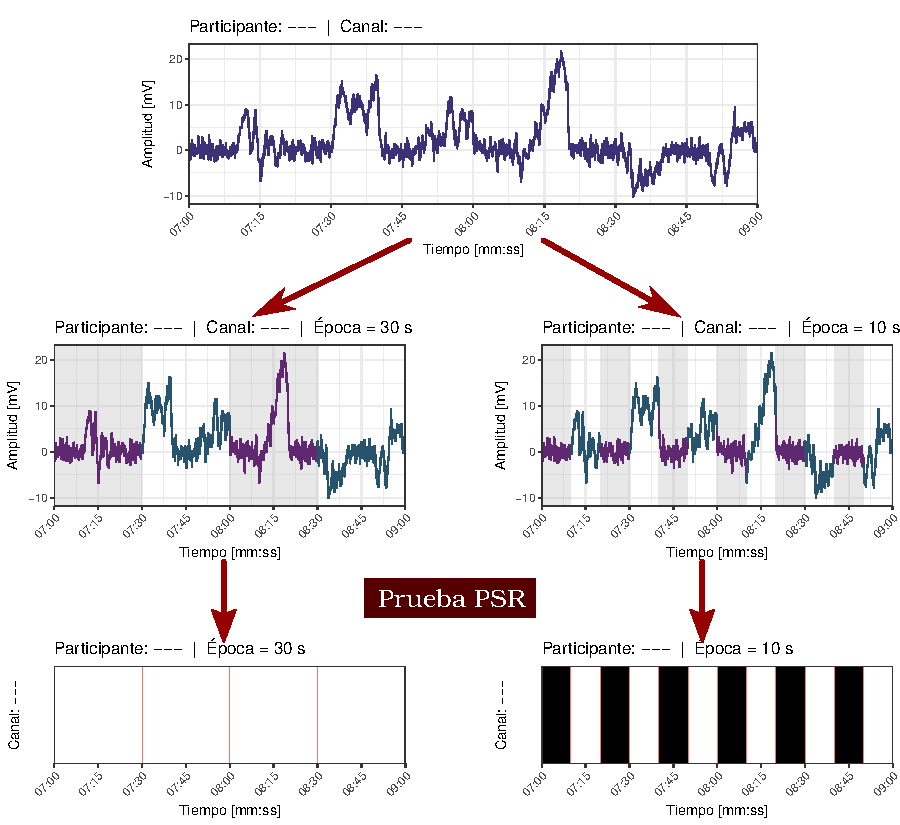
\includegraphics[width=\linewidth]{./img_diagramas/epocas_diferentes_v3.pdf}
\caption{Efecto del tamaño de ventana sobre la clasificación de estacionariedad.}
\label{epocas_diferentes}
\end{figure}

%%%%%%%%%%%%%%%%%%%%%%%%%%%%%%%%%%%%%%%%%%%%%%%%%%%%%%%%%%%%%%%%%%%%%%%%%%%%%%%%%%%%%%%%%%%%%%%%%%%
%%%%%%%%%%%%%%%%%%%%%%%%%%%%%%%%%%%%%%%%%%%%%%%%%%%%%%%%%%%%%%%%%%%%%%%%%%%%%%%%%%%%%%%%%%%%%%%%%%%
%%%%%%%%%%%%%%%%%%%%%%%%%%%%%%%%%%%%%%%%%%%%%%%%%%%%%%%%%%%%%%%%%%%%%%%%%%%%%%%%%%%%%%%%%%%%%%%%%%%
%%%%%%%%%%%%%%%%%%%%%%%%%%%%%%%%%%%%%%%%%%%%%%%%%%%%%%%%%%%%%%%%%%%%%%%%%%%%%%%%%%%%%%%%%%%%%%%%%%%

%%%%%%%%%%%%%%%%%%%%%%%%%%%%%%%%%%%%%%%%%%%%%%%%%%%%%%%%%%%%%%%%%%%%%%%%%%%%%%%%%%%%%%%%%%%%%%%%%%%
%%%%%%%%%%%%%%%%%%%%%%%%%%%%%%%%%%%%%%%%%%%%%%%%%%%%%%%%%%%%%%%%%%%%%%%%%%%%%%%%%%%%%%%%%%%%%%%%%%%
%%%%%%%%%%%%%%%%%%%%%%%%%%%%%%%%%%%%%%%%%%%%%%%%%%%%%%%%%%%%%%%%%%%%%%%%%%%%%%%%%%%%%%%%%%%%%%%%%%%

\chapter{Marco conceptual del problema}

Para poder identificar marcadores significativos para el diagnóstico del deterioro cognitivo, es 
posible usar la técnica de electroencefalografía, que es usada para medir cierto tipo de actividad 
cerebral y que posiblemente esté asociada al deterioro cognitivo. 
%
En esta sección se presenta el deterioro cognitivo en adultos mayores, con énfasis en su 
caracterización.

%%%%%%%%%%%%%%%%%%%%%%%%%%%%%%%%%%%%%%%%%%%%%%%%%%%%%%%%%%%%%%%%%%%%%%%%%%%%%%%%%%%%%%%%%%%%%%%%%%%
%%%%%%%%%%%%%%%%%%%%%%%%%%%%%%%%%%%%%%%%%%%%%%%%%%%%%%%%%%%%%%%%%%%%%%%%%%%%%%%%%%%%%%%%%%%%%%%%%%%

\section{Psicología}

La \textbf{demencia} es, según el Manual diagnóstico de y estadístico de trastornos mentales 
(DSM-V, por la versión consultada)
\begin{quote}
Un síndrome que consiste en el desarrollo de déficit cognoscitivos suficientemente graves como para 
interferir significativamente en las actividades laborales y sociales, respecto al nivel de 
actividad previo \cite{DCM5}.
%
Los sujetos con demencia tienen una baja capacidad para aprender información nueva y suelen olvidar 
lo aprendido anteriormente, siendo éste el síntoma más prominente.
\end{quote}

Cuando un sujeto presenta cambios marcados en su conducta, es relativamente fácil identificar la 
demencia; caso contrario es el diagnóstico temprano de la misma, el cual es importante para un 
tratamiento adecuado que revierta o desacelere el avance de este síndrome \cite{Knopman01}.

Considerando a los \textbf{adultos mayores} --entendidos como individuos de 60 años o más--
conviene mencionar que el envejecimiento es determinado por una serie de procesos moleculares, 
celulares, fisiológicos y psicológicos que conducen directamente al deterioro de funciones 
cognitivas, específicamente atención y memoria \cite{Park09}.
%
La funcionalidad durante esta etapa se relaciona con el estilo de vida, los factores de riesgo, el 
acceso a la educación y las acciones para el cuidado de la salud realizadas en edades más 
tempranas \cite{Sanhueza14}.

Al momento de diagnosticar deterioro cognitivo en adultos mayores, deben tenerse en cuenta el 
envejecimiento normal y la posible \textbf{pseudodemencia depresiva}, ya que presentan 
características similares. 
%
Con respecto a ésta última, definida como \textit{un trastorno del afecto y que produce un aparente 
deterioro cognitivo} \cite{DCM5}, aunque no se suele considerar como un tipo de demencia.

Así mismo, para realizar un diagnóstico temprano se considerará como etapa precursora de la 
demencia al \textbf{deterioro cognitivo leve}, definido como 
\begin{quote}
Una alteración adquirida y prolongada de una o varias funciones cognitivas, que no corresponde a un 
síndrome focal y no cumple criterios suficientes de gravedad para ser calificada como demencia
\cite{Robles02}.
\end{quote}
dentro del presente escrito, este síndrome será manejado como \textbf{posible deterioro cognitivo} 
(PDC) amén de que está etapa de daño se considera reversible.

%%%%%%%%%%%%%%%%%%%%%%%%%%%%%%%%%%%%%%%%%%%%%%%%%%%%%%%%%%%%%%%%%%%%%%%%%%%%%%%%%%%%%%%%%%%%%%%%%%%
%%%%%%%%%%%%%%%%%%%%%%%%%%%%%%%%%%%%%%%%%%%%%%%%%%%%%%%%%%%%%%%%%%%%%%%%%%%%%%%%%%%%%%%%%%%%%%%%%%%

\subsection{Psicometría}

En psicología los instrumentos de medición comunes son las \textbf{pruebas neuropsicológicas}, 
entendidas como muestras de alguna conducta de interés a las que se asignan puntajes para comparar 
cuantitativamente a los sujetos \cite{Ardila12}.
%
Es a través de estas herramientas que se declaran formalmente las deficiencias cognitivas o 
conductuales, así como su severidad y clasificación.

Las habilidades que se miden usando este tipo de pruebas se suelen agrupar en áreas o 
\textbf{dominios}: atención, lenguaje, cálculo, memoria y aprendizaje, percepción, motricidad, 
funciones somatosensoriales, habilidades espaciales, funciones ejecutivas, entre otros. 
%
La clasificación de dominios suele variar según algunos autores.

En el estudio realizado por Vázquez-Tagle en 2016 \cite{VazquezTagle16} se investigó el deterioro
cognitivo en el estado de Hidalgo, para lo cual se aplicó la siguiente batería de pruebas
neuropsicológicas:
\begin{itemize}
\item Estado cognoscitivo general
\begin{itemize}
\item {Evaluación Neuropsicológica (\textbf{Neuropsi})} \cite{Solis03}
\item {Mini Mental State Examination (\textbf{MMSE})} \cite{Velasco15}
\end{itemize}
\item Detectar pseudodemencia depresiva y ansiedad
\begin{itemize}
\item {Escala breve para la detección de ansiedad del anciano (\textbf{SATS})} \cite{Vargas11}
\item {Escala de Depresión Geriátrica (\textbf{GDS})} \cite{Yesavage82,Greenberg12}
\end{itemize}
\item Detectar cambios en la vida cotidiana
\begin{itemize}
\item {Escala sobre las actividades cotidianas de la vida diaria (\textbf{KATZ})} \cite{Roumec14}
\end{itemize}
\end{itemize}

%%%%%%%%%%%%%%%%%%%%%%%%%%%%%%%%%%%%%%%%%%%%%%%%%%%%%%%%%%%%%%%%%%%%%%%%%%%%%%%%%%%%%%%%%%%%%%%%%%%
%%%%%%%%%%%%%%%%%%%%%%%%%%%%%%%%%%%%%%%%%%%%%%%%%%%%%%%%%%%%%%%%%%%%%%%%%%%%%%%%%%%%%%%%%%%%%%%%%%%

\section{Fisiología}

El registro de la actividad eléctrica en el cerebro, referido como \textbf{electroencefalograma} 
(EEG), está tradicionalmente relacionado con la exploración de procesos mentales y sus trastornos; 
como ejemplo se puede citar que Hans Berger, reconocido como el inventor del EEG, reportó usar 
dicha técnica en 1932 para estudiar posibles cambios en un paciente con Alzheimer 
\cite{historia_eeg}.

El mecanismo base para la propoagación de campos eléctricos en las neuronas, depende de la 
capacidad de la membana celular para mantener un equilibrio estable de iones con el medio 
extracelular.
%
Dicho fenómeno fue ampliamente estudiado por Hodkin y Huxley y puede describirse brevemente de la 
siguiente manera: cuando existe un desequilibrio puntual y súbito en la concentración extracelular 
de iones, se bombean iones a través de la mebrana para reestablecer el equilibrio en tal punto; 
esta acción genera desequilibrios secundarios en regiones vecinas de la mebrana, que a su vez 
activan mecanismos similares. 
%
Como consecuencia, la perturbación en el potencial de membrana se propaga a lo largo de ésta y se 
genera la transmisión de impulsos nerviosos en neuronas.
%
Un excelente referente sobre el tema es el libro por Ermentrout \cite{Ermentrout10}.

El EEG mide indirectamente la transmisión de impulsos nerviosos entre neuronas de la corteza 
cerebral, de modo que constituye una medida del la \textit{cantidad} de actividad cerebral. 
%
La actividad registrada en el EEG consta principalmente de la actividad postsináptica de las 
neuronas piramidales en la corteza cerebral; éstas se encuentran altamente conectadas entre sí
forman capas densas.

%%%%%%%%%%%%%%%%%%%%%%%%%%%%%%%%%%%%%%%%%%%%%%%%%%%%%%%%%%%%%%%%%%%%%%%%%%%%%%%%%%%%%%%%%%%%%%%%%%%
%%%%%%%%%%%%%%%%%%%%%%%%%%%%%%%%%%%%%%%%%%%%%%%%%%%%%%%%%%%%%%%%%%%%%%%%%%%%%%%%%%%%%%%%%%%%%%%%%%%

\subsection{Polisomnografía}

Usualmente estos registros de EEG muestra una actividad oscilatoria continua y cambiante, cuya
frecuencia se considera entre 0.5 y 100 \hz. Su composición está fuertemente relacionada con el 
grado de actividad mental mostrando diferencias claras durante vigilia y sueño, o durante quietud 
y concentración \cite{Clark98_2}.

Aunque el EEG es irregular la mayor parte del tiempo, también muestra patrones relativamente 
organizadas conocidos como \textbf{ondas cerebrales}. 
%
Las ondas cerebrales más comunes y estudiadas se tipifican en cuatro grupos según su 
\textit{frecuencia}: alfa, beta, gamma, delta, theta.
%
En la figura \ref{ritmos} se representa un arquetipo visual de cada tipo de onda.

\begin{figure}
\centering
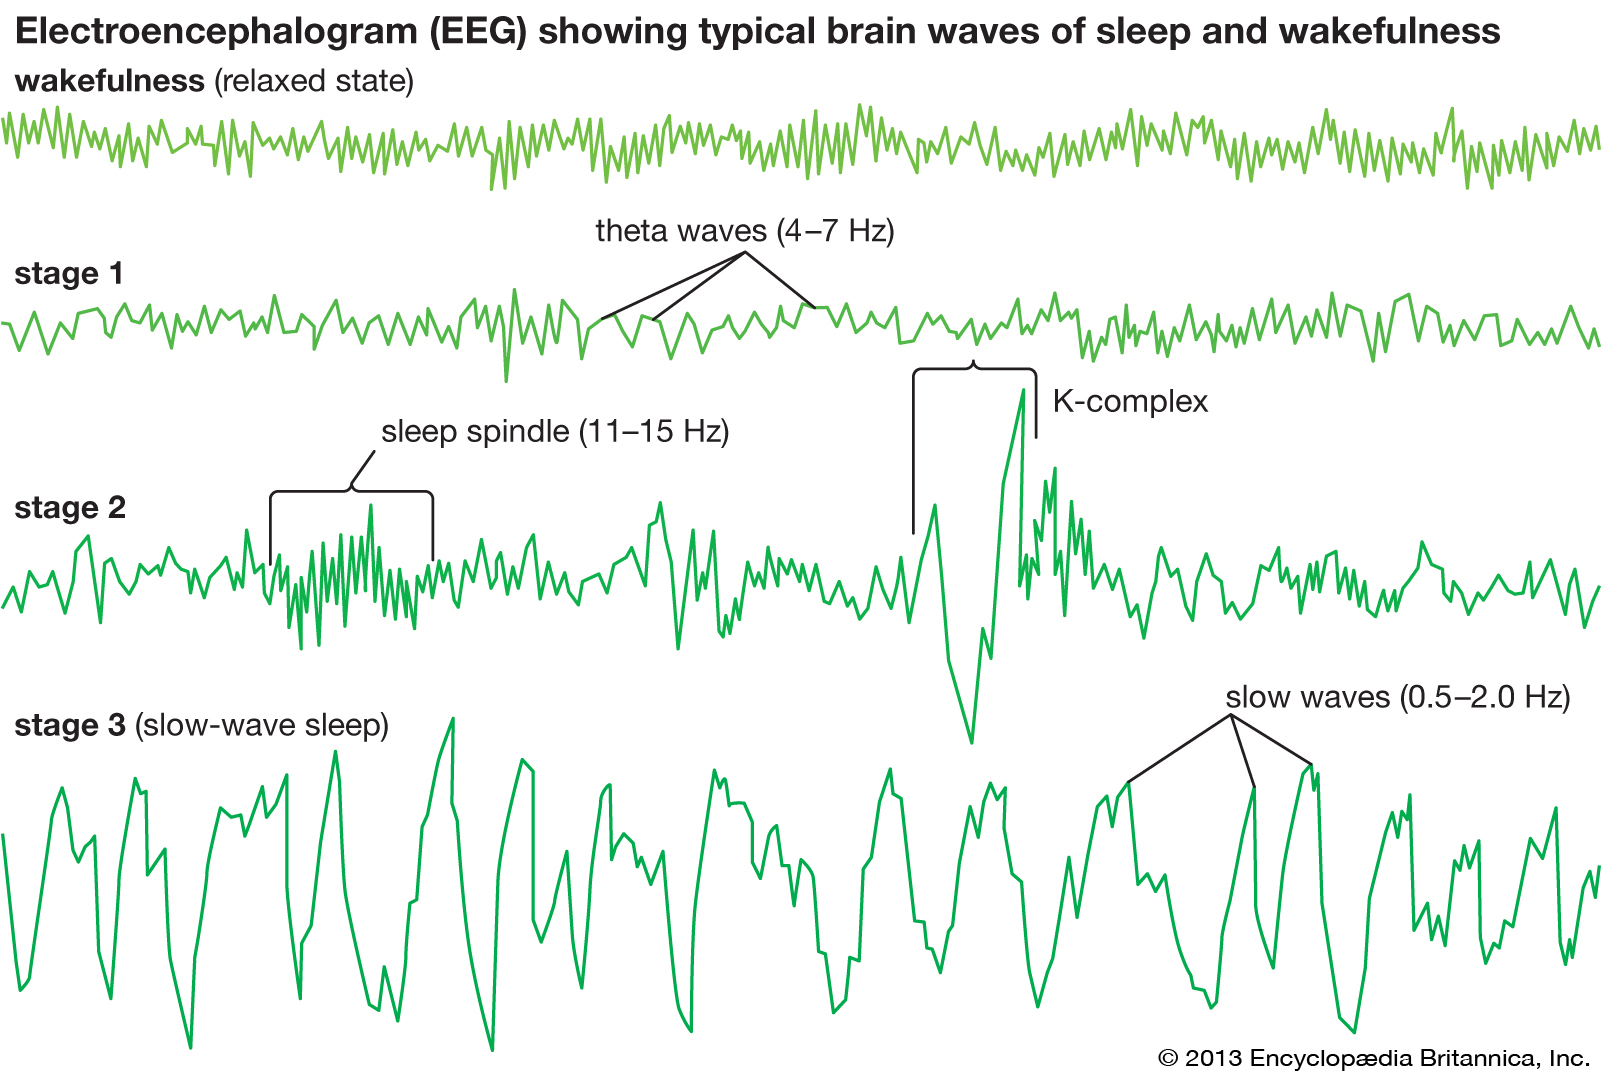
\includegraphics[width=0.95\linewidth]{./img_diagramas/ondas_britannica.jpg} 
\caption[Ejemplos de ondas cerebrales encontradas en el EEG]
{Ejemplos de ondas cerebrales encontradas en el EEG. Imagen tomada de Encyclop{\ae}dia Britannica, 
versión en línea \cite{Britannica}}
\label{ritmos}
\end{figure}

\begin{table}
\centering
\caption{Generalidades sobre ondas cerebrales}
{\small
\begin{tabular}{lclll}
\toprule
Tipo de onda & Frecuencia [\hz] & {Ubicación usual} & {Condiciones usuales} \\
\midrule
Delta & 0.5 -- 3.5 &         & Síndromes focales. Sueño \\
      &            &         & profundo en infantes \\
Theta & 3.5 -- 7   & P, T    & Durante estrés emocional \\
      &            &         & En infantes \\
Alfa  & 7 -- 12    & F, P, O & Vigilia en reposo con \\
      &            &         & ojos cerrados \\
Beta  & 12 -- 30   & P, F    &      Actividad mental en\\
      &            &         & adultos \\
Gamma & 30 -- 100  &         &\\
      &            &         & \\
%\midrule
%{Husos de} &&&\\
%sueño &&& \\
%{Complejo K} &&&\\
%&&& \\
\bottomrule
\end{tabular}\\
Se abrevian los lóbulos cerebrales: F=frontal, P=parietal, T=temporal, O=occipital
}
\label{tabla_ondas}
\end{table}

Para realizar el registro \textit{per se} en una forma estandarizada y comparable, se definen
arreglos llamados \textbf{montajes}, entendidos como el conjunto de (1) los sitios donde se colocan 
los electrodos de registro y (2) la manera en que los electrodos de registro están conectados entre 
sí.

En el trabajo de Vázquez Tagle \cite{VazquezTagle16} se usa un montaje \textit{referencial}, en el 
cual los electrodos se conectan en paralelo con un electrodo de referencia cuya actividad eléctrica 
es constante y negligible (lóbulos de las orejas, electrodos cortocircuitados A1, A2); los 
electrodos fueron colocados según el \textbf{Sistema 10--20} \cite{Jasper58,Klem99}.
%
Dicho sistema define los sitios según una cuadrícula construida respecto a distancias relativas 
entre varios puntos de referencia: el \textit{inion}, protuberancia la región posterior del cráneo, 
el \textit{nasión}, unión del hueso frontal y los huesos nasales, y el \textit{punto preauricular}, 
ubicado arriba del cartílago que protege el canal auditivo.

\begin{figure}
\centering
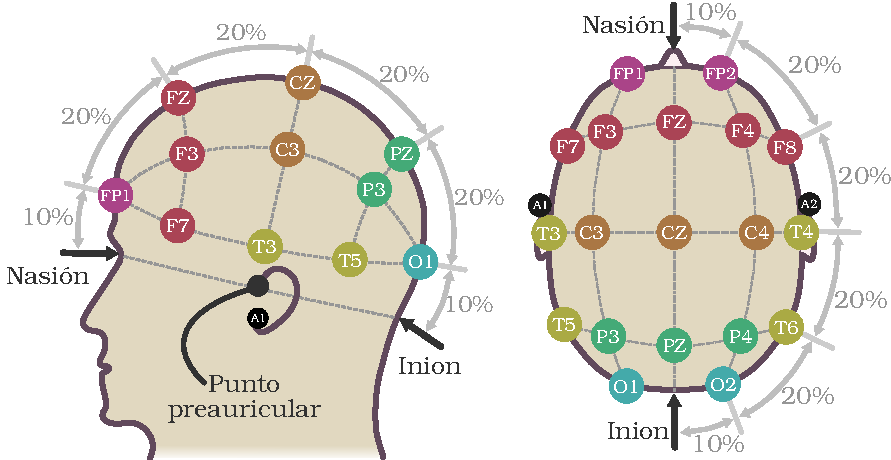
\includegraphics[width=\linewidth]{./img_diagramas/cabeza_proporcionada_color_v2.pdf} 
\caption{Colocación de electrodos según el sistema 10--20}
\label{img1020}
\end{figure}

Debido a que las neuronas en la corteza cerebral tienen orientaciones muy diversas y a que disparan 
de manera asíncrona, además de que el cerebro se encuentra cubierto por las muchas capas descritas
anteriormente, las señales captadas por los electrodos deben ser amplificadas analógicamente antes 
de ser registradas digitalmente.
%
A ello hay que añadir la difusión generada por las meninges, el líquido encefalorraquídeo y el 
cráneo.

Un efecto colateral de amplificar la señal es la inclusión de \textbf{ruido}, entendido como 
señales que son registradas de manera no deseada; como ejemplo, los músculos faciales medianamente 
contraídos generan campos eléctricos con frecuencia de 100 \hz.
%
Este tipo de ruido \textit{persistentes} son eliminados usando un filtro que \textit{elimine} los 
componentes de frecuencia específicos.
%
Los ruidos de duración corta son referidos como \textbf{artefactos}; como ejemplo, pestañear 
voluntariamente durante un episodio de quietud mental interrumpe las ondas alfa por cerca de dos 
segundos. 

Adicionalmente al registro del EEG, el PSG incluye el registro de algunas otras \textit{variables 
fisiológicas}, como respiración, ritmo cardiaco, temperatura, entre otros. 
%
En el estudio por Vázquez Tagle el registro de PSG fue complementado con registros de actividad 
ocular (\textbf{electrooculograma}, EOG) y tono muscular (\textbf{electromiograma}, EMG), según las 
recomendaciones de la AASM; la ubicación de los electrodos pertinentes es ilustrado en la figura 
\ref{emg_eog}.

\begin{figure}
\centering
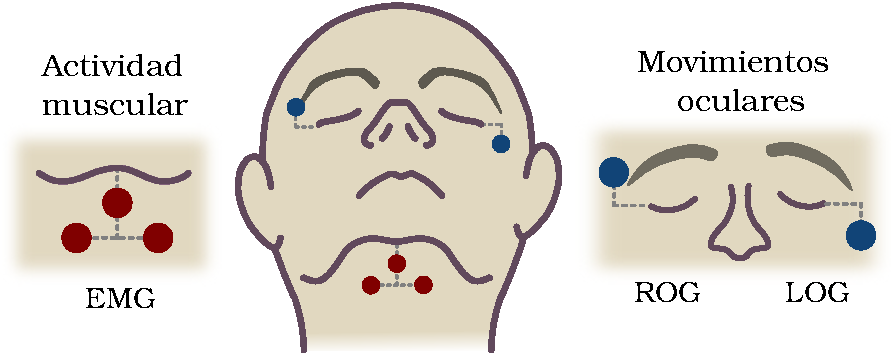
\includegraphics[width=\linewidth]
{./img_diagramas/emg_eog_v3.pdf}
\caption{Colocación de electrodos para registrar actividad ocular y tono muscular}
\label{emg_eog}
\end{figure}

Para interpretar los registros de EOG (canales LOG, ROG) se puede entender al ojo como una batería
cuyos  polos son la retina y la pupila, y que genera pequeñas variaciones en el campo eléctrico
cuando se mueve; el registro consiste en la proyección del movimiento sobre el eje que forman los
electrodos.
%
Los registros de EMG (canal EMG) admiten una interpretación más \textit{sencilla}, ya que los
músculos son activados directamente por señales eléctricas: el tono muscular es la actividad 
muscular basal, y se relaciona con la velocidad con que los músculos pueden \textit{salir} del 
reposo.

%%%%%%%%%%%%%%%%%%%%%%%%%%%%%%%%%%%%%%%%%%%%%%%%%%%%%%%%%%%%%%%%%%%%%%%%%%%%%%%%%%%%%%%%%%%%%%%%%%%
%%%%%%%%%%%%%%%%%%%%%%%%%%%%%%%%%%%%%%%%%%%%%%%%%%%%%%%%%%%%%%%%%%%%%%%%%%%%%%%%%%%%%%%%%%%%%%%%%%%

\subsection{Estructura del sueño}

Se entiende al sueño como un proceso vital, con una estructura característica, y que en el ser 
humano presenta las siguientes propiedades \cite{CarrilloMora}:
\begin{enumerate}
\item Disminución de conciencia y reactividad a estímulos externos
\item Fácilmente reversible, a diferencia de estados patológicos como estupor y coma
\item Inmovilidad y relajación muscular
\item Periodicidad típica circadiana (diaria)
\item Los individuos adquieren una postura estereotipada
\item La privación induce alteraciones conductuales y 
fisiológicas, además de que genera una \textit{deuda} acumulativa
\end{enumerate}

La duración del sueño es determinada en gran parte por la edad; el recién nacido duerme entre 14 y 
18 horas, el lactante entre 12 y 14 horas, el niño en etapa escolar entre 11 y 12 horas y en la 
edad adulta, la mayoría duerme entre 7 y 8 horas por noche \cite{Contreras13}.
%
Paralelemante el sueño no es un proceso homogéneo, sino que tiene una estructura por etapas con 
rasgos electroencefalográficos y fisiológicos distintivos.

Para su estudio, el sueño se divide en dos etapas: N y R.
%
La \textbf{fase N}, se caracteriza por movimientos oculares lentos, tono muscular que decrece 
constantemente, actividad cerebral que recuerda al reposo, y la presencia de husos de sueño y 
complejos K; en base a ello se divide en las sub-fases N1, N2, N3.

Durante la \textbf{fase R} el tono muscular disminuye (excepto para los músculos respiratorios y 
los esfínteres), la frecuencia cardiaca y respiratoria se vuelve irregular, y el sujeto exhibe 
movimientos oculares rápidos (MOR); en base a lo cual la fase R es conocida como \textbf{sueño 
MOR}.
%
En el EEG, aparecen ondas rápidas de bajo voltaje, irregulares, y que recuerdan la actividad 
durante el estado de alerta; estos patrones no interrumpen el sueño sino que, contrariamente,
incrementan el umbral para estímulos externos, motivo por el cual esta fase también es referida 
como \textbf{sueño paradójico}.
%
Cabe mencionar que durante el sueño MOR se producen la mayoría de las ensoñaciones (referidas 
coloquialmente como \textit{sueños}), y que la mayoría de los pacientes que despiertan durante esta 
fase suelen recordar vívidamente el contenido de sus ensoñaciones \cite{Rosales14}.

\begin{table}
\caption[Criterios para la clasificación de etapas de sueño]
{Criterios para la clasificación de etapas de sueño según la AASM}
\centering
{\small
\begin{tabular}{lllll}
\toprule
&&   & Movimientos & Tono \\
\multicolumn{2}{l}{Etapa}& Características del EEG & oculares & muscular \\
\midrule
Vigilia & W  & {Ritmo alfa} en $>50$\% de la época en   & No & Alto \\
        &    & la región occipital                &    &      \\
NMOR 1  & N1 & Cambio de alfa por AABFM, atenuación & Lentos & $<$W     \\
        &    & del ritmo dominante. Ondas agudas   &    &      \\
NMOR 2  & N2 & Husos de sueño y complejos K en la    & No & $<$W, $>$R     \\
        &    & primera mitad de la época. AABFM &    &     \\
NMOR 3  & N3 & {Ondas lentas} (0.5--2 \hz, $>75$ \mv) en& No & $<$N2, $\approx$R \\
        &    & $>20$\% de la época. Husos de sueño       &&      \\
MOR     & R  & Actividad baja amplitud y frecuencias & MOR's & Bajo  \\
        &    & mixtas. Ondas 'saw-tooth'             &       &       \\
\bottomrule
\multicolumn{4}{l}{Se abrevia AABFM=Actividad de Amplitud Baja y Frecuencias Mixtas}
\end{tabular}\\
}
\end{table}

\begin{figure}
\centering
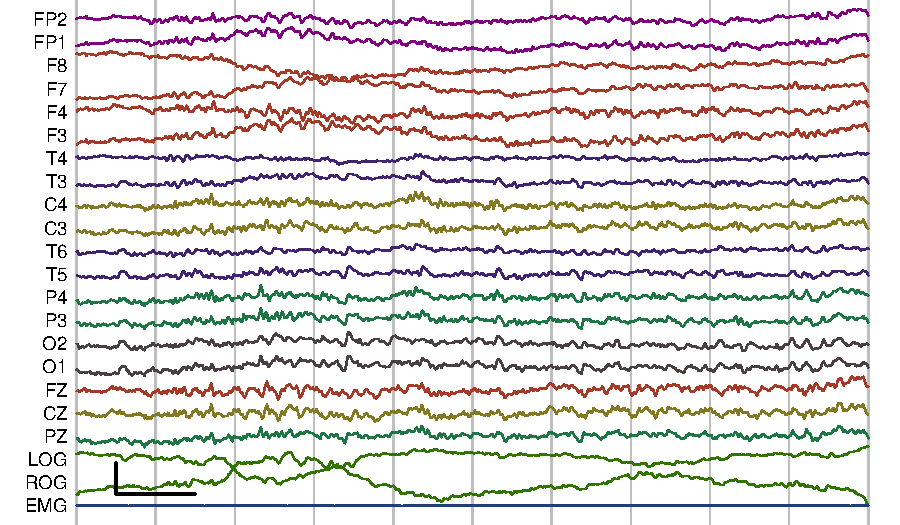
\includegraphics[width=\linewidth]
{./img_ejemplos/MJNN_epoca_stam.pdf}
\caption[Registro de polisomnograma durante sueño MOR]
{Registro de polisomnograma durante sueño MOR. Marca de calibración: vertical, 10 \mv, horizontal, 
1 segundo}
\label{ejemplos_mor}
\end{figure}

%%%%%%%%%%%%%%%%%%%%%%%%%%%%%%%%%%%%%%%%%%%%%%%%%%%%%%%%%%%%%%%%%%%%%%%%%%%%%%%%%%%%%%%%%%%%%%%%%%%
%%%%%%%%%%%%%%%%%%%%%%%%%%%%%%%%%%%%%%%%%%%%%%%%%%%%%%%%%%%%%%%%%%%%%%%%%%%%%%%%%%%%%%%%%%%%%%%%%%%
%%%%%%%%%%%%%%%%%%%%%%%%%%%%%%%%%%%%%%%%%%%%%%%%%%%%%%%%%%%%%%%%%%%%%%%%%%%%%%%%%%%%%%%%%%%%%%%%%%%

%%%%%%%%%%%%%%%%%%%%%%%%%%%%%%%%%%%%%%%%%%%%%%%%%%%%%%%%%%%%%%%%%%%%%%%%%%%%%%%%%%%%%%%%%%%%%%%%%%%
%%%%%%%%%%%%%%%%%%%%%%%%%%%%%%%%%%%%%%%%%%%%%%%%%%%%%%%%%%%%%%%%%%%%%%%%%%%%%%%%%%%%%%%%%%%%%%%%%%%
%%%%%%%%%%%%%%%%%%%%%%%%%%%%%%%%%%%%%%%%%%%%%%%%%%%%%%%%%%%%%%%%%%%%%%%%%%%%%%%%%%%%%%%%%%%%%%%%%%%

\chapter{Metodología y resultados}
\label{ch:metodologia}

El presente trabajo surge de una colaboración con el Laboratorio de Sueño, Emoción y Cognición, dependiente del Instituto de Ciencias de la Salud de la UAEH y a cargo de la Dra. Alejandra Rosales Lagarde.
%
La colaboración incluye acceso a los registros obtenidos en un estudio por Vázquez-Tagle en 2016 \cite{VazquezTagle16}. 
%
Dicho estudio se centró en la epidemiología de los trastornos del sueño en adultos mayores dentro del estado de Hidalgo, y consideró registros de PSG para evaluar parámetros relacionados al sueño MOR.
%
El presente trabajo tiene como objetivo particular analizar con mayor detalle dichos registros.

En este capítulo se describe primeramente la metodología seguida para obtener los registros de PSG.
%
Posteriormente se describe la metodología usada para analizar los registros de PSG, usando las herramientas descritas en el capítulo \ref{capitulo:espectro_evo}.

Los registros de PSG fueron segmentados en ventanas de 30 segundos, referidas como \textbf{épocas}.
%
El análisis de los registros de PSG se llevó a cabo a tres niveles:
\begin{itemize}
\item Dentro de cada época.
\item Entre las diferentes épocas en un registro.
\item Entre los diferentes participantes.
\end{itemize}

El análisis a nivel de época contempla su clasificación según etapa de sueño (limitada a MOR y NMOR), y su clasificación como estacionarias (usando la prueba de PSR).
%
El uso de épocas como unidades de estudio se justifica por la gran heterogeneidad del sueño nocturno; paralelamente, destaca el supuesto fisiológico de que las etapas de sueño son \textit{comunes} entre los humanos.
%
En suma, los registros de PSG para un sólo individuo pueden interpretarse como una población de épocas.

El análisis a nivel de registro surge de considerar la heterogeneidad del sueño pero usando al registro entero como unidad de estudio.
%
El tomar las épocas junto con su estructura temporal reveló algunos patrones interesantes de actividad.

Para el análisis entre participantes (divididos en grupos), varias de las características descritas fueron \textit{colapsadas} para constituir características \textit{simples}. 
%
Debido a las características de la muestra (ver más adelante), los resultados obtenidos no pueden extrapolarse a la población en general.
%
Los resultados obtenidos, entonces, se presentan como \textit{indicios}.

%%%%%%%%%%%%%%%%%%%%%%%%%%%%%%%%%%%%%%%%%%%%%%%%%%%%%%%%%%%%%%%%%%%%%%%%%%%%%%%%%%%%%%%%%%%%%%%%%%%

\section{Características de los participantes}

Los participantes fueron elegidos usando un muestreo \textit{no probabilístico por conveniencia} bajo los siguientes criterios de inclusión:
\begin{itemize}
\item Edad entre 60 y 85 años
\item Diestros (mano derecha dominante)
\item Sin ansiedad, depresión ni síndromes focales
\item No usar medicamentos o sustancias para dormir
\item Firma de consentimiento informado
\item Voluntario para el registro de PSG
\end{itemize}

Un total de 16 adultos mayores cumplieron los criterios de inclusión. 
%
Con el fin de detectar el DCL en estos pacientes, éstos fueron sometidos a una batería de pruebas neuropsicológicas para determinar su estado cognoscitivo general (Neuropsi, MMSE), detectar cambios en su vida cotidiana (KATZ) y descartar cuadros depresivos (SAST, GDS); para más detalles ver capítulo anterior, sección \ref{seccion:pruebas}.
%
En la tabla \ref{puntajes} se reportan los puntajes obtenidos por los participantes en dichas pruebas; estos datos deben ser interpretados según los \textit{puntajes de corte} de cada prueba, que se incluyen en el apéndice \ref{apendice_pruebas}.
%reportados en las tablas \refrange{anexo:sast_gds,anexo:mmse,anexo:neuropsi,anexo:katz}.
% \crefrange{anexo:sast_gds,anexo:mmse,anexo:neuropsi,anexo:katz}.
%
Se determinó que 11 de los voluntarios no padecen depresión o ansiedad, ni presentan afectaciones significativas en la vida diaria; el participante MGG presenta un cuadro depresivo, pero fue incluido en ausencia de afecciones cognitivas objetivas.
%
Debido a motivos técnicos, sólo 9 participantes fueron considerados para el presente trabajo; se reportan únicamente los datos relativos a esos participantes.

En base al diagnóstico de Posible Deterioro Cognitivo Leve, los 9 participantes fueron divididos en dos grupos: PDCL y CTRL. 
%
Es importante mencionar que, bajo las condiciones muestrales, el grupo CTRL no puede fungir satisfactoriamente como grupo control; una descripción más adecuada sería \textit{grupo sin PDCL}.

%Para esta clasificación se dio mayor atención al puntaje de Neuropsi, estandarizado según edad y 
%escolaridad (cuadro \ref{puntajes}). 
%
%Cabe mencionar que intencionalmente se dio menor importancia a los puntajes de la prueba MMSE en cuanto al diagnóstico del PDCL; ésto porque se ha reportado que, en la población mexicana, esa prueba tiene baja sensibilidad para el diagnóstico de DCL en general, y baja especificidad para individuos con escolaridad muy baja o muy alta \cite{Ostrosky00}.
%%
%Para fines del comentario anterior, se entiende por \textit{sensibilidad} a la probabilidad de obtener verdaderos positivos, y por \textit{especificidad} a la probabilidad de obtener verdaderos negativos.

\begin{table}
\caption{Datos generales de los participantes}
\centering
\bordes{1.1}
{\small
\begin{tabular}{llcrrrrrrr}
\toprule
 \phantom{mmm}&
 & {Sexo} & {Edad} & {Escol.} & {Neuropsi} & {MMSE} & {SAST} & {KATZ} & {GDS} \\
\midrule
\multicolumn{2}{l}{\textbf{Grupo CTRL}}\\
&MJH    & F    & 72\pz & 9\pz  & 113\pz & 30\pz & 18\pz & 0\pz & 0\pz  \\
&JAE    & F    & 78\pz & 5\pz  & 102\pz & 28\pz & 19\pz & 0\pz & 5\pz  \\
&MGG    & F    & 61\pz & 9\pz  & 114\pz & 28\pz & 29\pz & 1\pz & 14\pz \\
&EMT    & F    & 50\pz & 22\pz & 117\pz & 30\pz & 15\pz & 0\pz & 4\pz  \\
\rowcolor{gris}
&\multicolumn{1}{c}{$\widehat{\mu}$} & 
               & 65.3  & 11.3  & 111.5  & 29.0  & 20.3  & 0.3  & 5.8  \\
\rowcolor{gris}
&\multicolumn{1}{c}{$\widehat{\sigma}$} & 
               & 12.4  & 7.4   & 6.6    & 1.2   & 6.1   & 0.5  & 5.9  \\
\midrulec
%\hline
\multicolumn{2}{l}{\textbf{Grupo PDCL}}\\
& CLO   & F    & 68\pz &  5\pz &  81\pz & 28\pz & 22\pz & 1\pz &  6\pz \\
& RLO   & F    & 63\pz &  9\pz &  90\pz & 29\pz & 20\pz & 0\pz &  3\pz \\
& JGZ   & M    & 65\pz & 11\pz &  87\pz & 25\pz & 20\pz & 0\pz &  1\pz \\
& AEFP  & M    & 73\pz &  8\pz &  96\pz & 29\pz &   \pz & 0\pz &  2\pz \\
& PCM   & M    & 71\pz &  9\pz & 111\pz & 28\pz & 20\pz & 0\pz & 10\pz \\
\rowcolor{gris}
&\multicolumn{1}{c}{$\widehat{\mu}$} & 
              &  68.0  & 8.4   & 93.0   & 27.8  & 20.5  & 0.2  & 4.4  \\
\rowcolor{gris}
&\multicolumn{1}{c}{$\widehat{\sigma}$} & 
              & 4.1    & 2.2   & 11.4   & 1.6   & 1.0   & 0.4  & 3.6 \\
\bottomrulec
\end{tabular} 
}
\label{tab_sujetos}
\end{table}

%%%%%%%%%%%%%%%%%%%%%%%%%%%%%%%%%%%%%%%%%%%%%%%%%%%%%%%%%%%%%%%%%%%%%%%%%%%%%%%%%%%%%%%%%%%%%%%%%%%
%%%%%%%%%%%%%%%%%%%%%%%%%%%%%%%%%%%%%%%%%%%%%%%%%%%%%%%%%%%%%%%%%%%%%%%%%%%%%%%%%%%%%%%%%%%%%%%%%%%

\subsection{Registro del polisomnograma}

Para efectuar el registro de la PSG, los participantes acudieron a las instalaciones del Laboratorio de Sueño, Emoción y Cognición. 
%
Los participantes recibieron instrucciones de realizar una rutina normal de actividades durante la semana que precedió al estudio, y se les recomendó no ingerir bebidas alcohólicas o energizantes (como café o refresco) durante las 24 horas previas al experimento, y que no durmieran siesta ese día.
%
Bajo estas condiciones experimentales se garantiza que los registros son representativos del sueño nocturno de cada participante.

El registro per se fue efectuado usando un polisomnógrafo Medicid 5 (Neuronic Mexicana). El protocolo de la PSG incluye los siguientes electrodos\footnote{Para más detalles ver el capítulo anterior, particularmente la sección \ref{capitulo:psg}}:
\begin{itemize}
\item 19 electrodos de EEG colocadas según el Sistema Internacional 10--20.
\item 2 electrodos de EOG para movimientos oculares.
\item 2 electrodos de EMG para tono muscular en los músculos submentonianos.
\end{itemize}

Los electrodos para EEG fueron conectados en paralelo usando como referencia común los lóbulos de las orejas; se mantuvo por debajo de \SI{50}{\micro\ohm}.
%
Las señales fueron amplificadas analógicamente usando amplificadores de alta ganancia en cadena, 
y adicionalmente fueron \textit{pasado} filtros analógicos pasa bandas: 0.1--100 Hz 
para EEG, 3--20 Hz para EOG. 
%
Los registros fueron digitalizados con una frecuencia de muestreo de 512 puntos por segundos (Hz), y posteriormente almacenados en formato de texto bajo la codificación ASCII.

Como se mencionó anteriormente, los registros fueron segmentados en segmentos de 30 segundos, referidas como \textbf{épocas}; en lo posterior se usará la palabra `época' como un caso particular de ventana.
%
Cada una de las épocas fue clasificada como MOR o NMOR; la clasificación fue llevada a cabo por dos expertos de ICSA, y bajo los estándares de la AASM.

Por simplicidad técnica, los registros fueron truncados para poder considerar épocas completas; algunos datos al final de cada registro fueron omitidos, aunque representan una cantidad negligible de tiempo.
%
Cabe mencionar que cada época de 30 segundos, a una frecuencia de 512 Hz, representa un total de 15,360 puntos.

En la tabla \ref{tab:psg} se describe la duración de los registros, así como la cantidad de tiempo del registro clasificado como sueño MOR.
%
La cantidad de tiempo en vigilia registrado es negligible ($<5$ minutos por cada participante), de modo que ésta no es reportada; con una pérdida mínima de generalidad, se puede afirmar que los registros fuera del sueño MOR corresponden a sueño NMOR.

\begin{table}
\centering
\caption{Datos generales sobre los registros de PSG}
\bordes{1.2}
\begin{tabular}{llllcllr}
\toprule
    \phantom{mmm}&
    & \multicolumn{2}{l}{Total} & \phantom{l}   & \multicolumn{3}{l}{MOR*}\\
    \cmidrule{3-4}  \cmidrule{6-8}
    &          &Épocas  &  Tiempo   &&Épocas  &  Tiempo   &  \% \\
\midrule
\multicolumn{2}{l}{\textbf{Grupo CTL}}\\
&MJH &    1032   &      8:36:00  &&    127   &   1:03:30 &12.31 \\
&JAE &\ppu 904   &      7:32:00  &&    171   &   1:25:30 &18.92 \\
&MGG &    1024   &      8:32:00  &&    166   &   1:23:00 &16.21 \\
&EMT &\ppu 552   &      4:36:00  &&\ppu 47   &   0:23:00 & 8.51 \\
 
\rowcolor{gris}
&\multicolumn{1}{c}{$\widehat{\mu}$}  
     &\ppu 878.0 &      7:19:00 &&    128.0 &   1:03:53&13.99 \\
\rowcolor{gris}
&\multicolumn{1}{c}{$\widehat{\sigma}$} 
     &\ppu 225.1 &      1:52:32 &&\ppu 57.3  &   0:28:39&4.55 \\ 
\midrulec

\multicolumn{2}{l}{\textbf{Grupo PDC}}\\
&CLO  &\ppu 944   &\ppu 7:52:00 &&    132   &   1:06:00 & 13.98 \\
&RLO  &\ppu 840   &\ppu 7:00:00 &&\ppu 99   &   0:49:30 & 11.79 \\
&JGZ  &    1200   &    10:00:00 &&\ppu 34   &   0:17:00 &  2.83 \\
&AEFP &\ppu 952   &\ppu 7:56:00 &&\ppu 41   &   0:20:00 &  4.31 \\
&PCM  &\ppu 752   &\ppu 6:16:00 &&\ppu 59   &   0:29:30 &  7.85 \\
 
\rowcolor{gris}
&\multicolumn{1}{c}{$\widehat{\mu}$}  
      &\ppu 937.6 &\ppu 7:48:48 &&\ppu 73.0 &   0:36:30 & 8.15 \\
\rowcolor{gris}
&\multicolumn{1}{c}{$\widehat{\sigma}$} 
      &\ppu 168.1 &\ppu 1:24:04 &&\ppu 41.5 &   0:20:46 & 4.75 \\
\bottomrulec
\end{tabular}\\
*El sueño MOR aparece fragmentado, se reporta la suma de tales tiempos
\label{tab:psg}
\end{table}

%%%%%%%%%%%%%%%%%%%%%%%%%%%%%%%%%%%%%%%%%%%%%%%%%%%%%%%%%%%%%%%%%%%%%%%%%%%%%%%%%%%%%%%%%%%%%%%%%%%
%%%%%%%%%%%%%%%%%%%%%%%%%%%%%%%%%%%%%%%%%%%%%%%%%%%%%%%%%%%%%%%%%%%%%%%%%%%%%%%%%%%%%%%%%%%%%%%%%%%

\section{Características muestrales}

Previo a los análisis de los registros de PSG, se corroboró si los dos grupos de participantes efectivamente se \textit{comportan} como grupos estadísticamente diferentes.
%
Con dicho objetivo, se aplicaron pruebas $U$ de Wilcoxon-Mann-Whithney (WMW) entre los dos grupos, para todas las variables consideradas. 
%
De lo anterior se exceptúa al puntaje de la prueba KATZ, ya que es un parámetro cualitativo. 
%
Se concluye que las mediciones son parecidas en ambos grupos para todas las variables observadas, excepto para el puntaje en la prueba Neuropsi; ello era de esperarse ya que el puntaje en Neuropsi fue usado para designar a los participantes en los grupos.
%
Los resultados de estas pruebas se reportan en la tabla \ref{tab:var_wilcox}.

\begin{table}
\centering
\caption{Variables independientes entre grupos}
\begin{tabular}{lrlcrlcccr}
\toprule
 & \multicolumn{2}{l}{Grupo CTRL} & \phantom{.} & \multicolumn{2}{l}{Grupo PDCL} 
 & \phantom{.} & \multicolumn{2}{l}{Prueba de WMW}
 \\
\cmidrule{2-3} \cmidrule{5-6} \cmidrule{8-9}
& Media & (DE) & & Media & (DE) & & $p$ & $W$ \\
\midrule
Edad          & 65.3     & 12.4     &      & 68.0     & 4.1      &        & 0.905 & 9.0  \\
Escolaridad   & 11.3     & 7.4      &      & 8.4      & 2.2      &        & 0.797 & 11.5 \\
Neuropsi      & 111.5    & 6.6      &      & 93.0     & 11.4     &        &\bf 0.032 & 19.0 \\
MMSE          & 29.0     & 1.2      &      & 27.8     & 1.6      &        & 0.366 & 14.0 \\
SATS          & 20.3     & 6.1      &      & 20.5     & 1.0      &        & 0.301 & 4.0  \\
GDS           & 5.8      & 5.9      &      & 4.4      & 3.6      &        & 0.905 & 11.0 \\
Sueño {[}s{]} & 7:19:00  & 1:52:32  &      & 7:48:48  & 1:24:04  &        & 1.000 & 10.0 \\
MOR {[}s{]}   & 1:03:52  & 0:28:39  &      & 0:36:30  & 0:20:46  &        & 0.190 & 16.0 \\
MOR {[}\%{]}  & 14.0\%   & 4.5\%    &      & 8.2\%    & 4.8\%    &        & 0.111 & 17.0 \\
\bottomrule 
\multicolumn{8}{l}{DE=Desviación Estándar, WMW=Wilcoxon--Mann--Whitney}
\end{tabular} 
\label{tab:var_wilcox}
\end{table}

Se verificó si hay correlaciones entre las variables consideradas, lo cual podría afectar la interpretación de los resultados posteriores.
%
Para ello se aplicó la prueba de correlación de Spearman a cada par de variables; para la prueba de Spearman estima de la correlación entre variables, y se prueba la hipótesis de que la correlación es diferente de cero.
%
Estos resultados se reportan en el cuadro \ref{tab:correlacion}.

\begin{table}
\centering
\caption{Prueba de correlación de Spearman (estimación y p-valor)}
\begin{tabular}{ccccccccc}
\toprule
             & \rotatebox{90}{Escolaridad} & \rotatebox{90}{Neuropsi} & \rotatebox{90}{MMSE} & \rotatebox{90}{SAST} & \rotatebox{90}{GDS} & \rotatebox{90}{Sueño [s]} & \rotatebox{90}{MOR [s]} & \rotatebox{90}{MOR [\%]} \\
\midrule
Edad     & -0.699 & -0.267 & -0.079 & -0.171 & -0.233 & 0.200  & 0.183  & 0.100   \\
         & (\textbf{0.04}) & (0.49) & (0.84) & (0.69) & (0.55) & (0.61) & (0.64) & (0.81)  \\
\rowcolor{gris}
Escol.   &        & 0.437  & 0.194  & -0.366 & -0.254 & -0.044 & -0.586 & -0.525  \\
\rowcolor{gris}
         &        & (0.24) & (0.62) & (0.37) & (0.51) & (0.91) & (0.10) & (0.15)  \\

Neuropsi &        &        & 0.501  & -0.415 & 0.200  & -0.267 & 0.150  & 0.200   \\
         &        &        & (0.17) & (0.31) & (0.61) & (0.49) & (0.71) & (0.61)  \\

\rowcolor{gris}
MMSE     &        &        &        & -0.628 & -0.378 & -0.316 & -0.070 & 0.018   \\
\rowcolor{gris}
         &        &        &        & (0.09) & (0.32) & (0.41) & (0.86) & (0.96)  \\

SATS     &        &        &        &        & 0.610  & 0.317  & 0.293  & 0.195   \\
         &        &        &        &        & (0.11) & (0.44) & (0.48) & (0.64)  \\

\rowcolor{gris}
GDS      &        &        &        &        &        & -0.433 & 0.517  & 0.467   \\
\rowcolor{gris}
         &        &        &        &        &        & (0.25) & (0.16) & (0.21)  \\

Sueño [s]&        &        &        &        &        &        & -0.050 & -0.067  \\
         &        &        &        &        &        &        & (0.91) & (0.88)  \\

\rowcolor{gris}
MOR [s]  &        &        &        &        &        &        &        & 0.983   \\
\rowcolor{gris}
         &        &        &        &        &        &        &        & (\textbf{0.00})  \\
%\bottomrule
\bottomrulec
%\multicolumn{7}{l}{Niveles de significancia: *$<$.05 , **$<$.01 , ***$<$.005 , ****$<$.001}
\end{tabular}
\label{tab:correlacion}
\end{table}

Sólo se encontraron correlaciones significativas entre dos pares de variables: edad y escolaridad, y tiempo en MOR \textit{medido} en segundos y en porcentaje.

La primera relación, no muy fuerte, puede explicarse como un \textit{efecto generacional}: la educación superior ha aumentado su cobertura durante las últimas décadas, y entonces los grupos poblacionales más jóvenes tienen en promedio más años de escolaridad. 
%
%En base a estudios horizontales de larga escala, algunos autores han sugerido que un bajo nivel de escolaridad es un factor de riesgo para padecer deterioro cognitivo \cite{Mejia_Arango2007}.
%
Una segunda hipótesis para esta correlación es la contribución del participante EMT, quien tiene una edad menor y un nivel de educación mayor al resto de los participantes.
%
Para contrastar la segunda hipótesis se calculó nuevamente la prueba de Spearman pero retirando los datos de EMT: se halló una correlación estimada de 0.179 con un p-valor asociado de 0.672, que no permite rechazar el que la correlación sea diferente de cero.

Se descarta entonces la hipótesis del efecto generacional, cuando menos para el grupo de participantes considerados, y se acepta que la correlación es debida a valores atípicos. Se concluye que, usando los datos recabados, no se pueden obtener información relevante sobre el efecto del nivel de educación ni la edad sobre el PDCL, ni con los marcadores del PSG que se describirán más adelante.

Intuitivamente era de esperarse la correlación entre el tiempo en MOR y el porcentaje de sueño que es MOR.
%
Sin embargo, la hipótesis de que el sueño tenga una \textit{estructura característica} --y por tanto, que las etapas de sueño aparezcan en proporciones similares en varios individuos--- es ajena a los supuestos estadísticos.
%
Con base a este resultado, en adelante se usará el porcentaje de MOR como \textit{sustituto} del tiempo real de MOR porque (1) dichas variables están fuertemente correlacionadas, y (2) porque el porcentaje permite comparar intuitivamente a características de registros con duraciones muy diferentes.

%%%%%%%%%%%%%%%%%%%%%%%%%%%%%%%%%%%%%%%%%%%%%%%%%%%%%%%%%%%%%%%%%%%%%%%%%%%%%%%%%%%%%%%%%%%%%%%%%%%
%%%%%%%%%%%%%%%%%%%%%%%%%%%%%%%%%%%%%%%%%%%%%%%%%%%%%%%%%%%%%%%%%%%%%%%%%%%%%%%%%%%%%%%%%%%%%%%%%%%

\section{Análisis a nivel de época}
\label{sec:analisis_epoca}

Como se mencionó anteriormente, los registros fueron fragmentados en ventanas de 30 segundos, referidas como épocas, para su clasificación en etapa de sueño.
%
De manera independiente, cada una de estas épocas fue sometida a la prueba de estacionariedad de Prietley--Subba Rao (PSR) para investigar si es estacionaria en el sentido de homogeneidad espectral; para más detalles ver la sección \ref{sec:psr}.

En base a la prueba de PSR, cada una de las épocas consideradas fue clasificada como \textit{estacionaria} 
si fue rechazada la hipótesis de no--estacionariedad con un nivel de significancia $p<0.05$.
%
La aplicación per se de la prueba de PSR fue efectuada usando el software estadístico R; en particular, se utilizó la implementación incluida en el paquete \texttt{fractal} bajo la función \texttt{stationarity} \cite{R_fractal}.

Con cada época clasificada según etapa de sueño (MOR o NMOR) y según estacionariedad, se procedió primeramente a revisar cómo están relacionadas ambas características.
%
Para ello se planteó la hipótesis de que la cantidad de épocas estacionarias es diferente en MOR y NMOR. 
%
Debido a que la cantidad de épocas en NMOR es considerablemente mayor a las épocas en MOR, y en base a las observaciones de la sección anterior, se usaron proporciones en lugar del total de épocas;
para simplificar la referencia, las proporciones de épocas clasificadas como estacionarias en MOR y NMOR serán referidas como $\text{p}_{\text{MOR}}$ y $\text{p}_{\text{NMOR}}$, respectivamente.
%
Dado que ambas clasificaciones son dicotómicas, la hipótesis $\text{p}_{\text{MOR}}\neq\text{p}_{\text{NMOR}}$ fue probada usando la prueba $\chi^{2}$ de Pearson para cada sujeto en todas las derivaciones consideradas.

Los resultados obtenidos se reportan en el apéndice \ref{apendiceA}, y en la figura \ref{cabeza_new} se muestra de forma esquemáticamente en qué derivaciones se encontraron diferencias significativas.
%
No se encontraron patrones claros que pudieran relacionar el PDCL --ni otros factores considerados-- con las regiones con diferencias significativas.

\begin{figure}
\centering
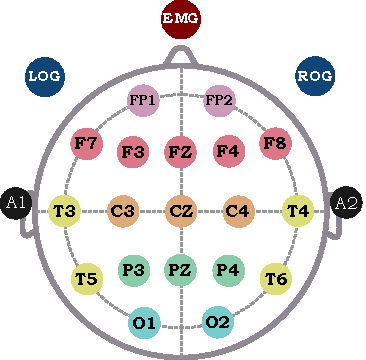
\includegraphics[scale=1.2]
{./img_diagramas/estampa_v1.pdf}
\caption{Representación minimalista de los electrodos considerados en el registro de PSG;
%: 19 para el EEG, dos para el EOG, un grupo de 3 para el EMG y dos electrodos de referencia.
para más detalles ver las secciones \ref{sec:eeg} y \ref{sec:emg_eog}.
Esta forma de ordenar las gráficas será usado en gráficos posteriores.}
\label{img:estampa}
\end{figure}

\begin{figure}
\centering
\begin{tabular}{c}
\begin{tabular}{cccc}
MJH & JAE & MGG & EMT \\
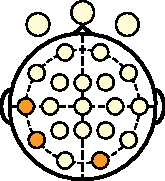
\includegraphics[width=0.17\textwidth]{./img_art_dfa/prop_MJH_30.pdf} &
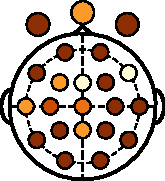
\includegraphics[width=0.17\textwidth]{./img_art_dfa/prop_JAE_30.pdf} &
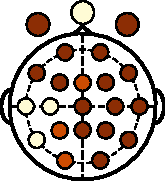
\includegraphics[width=0.17\textwidth]{./img_art_dfa/prop_MGG_30.pdf} &
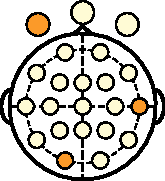
\includegraphics[width=0.17\textwidth]{./img_art_dfa/prop_EMT_30.pdf} \\
\end{tabular} \\
\midrule
\begin{tabular}{ccccc}
CLO & RLO & JGZ & AEFP & PCM \\
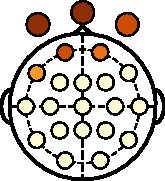
\includegraphics[width=0.17\textwidth]{./img_art_dfa/prop_CLO_30.pdf} &
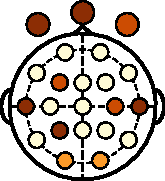
\includegraphics[width=0.17\textwidth]{./img_art_dfa/prop_RLO_30.pdf} &
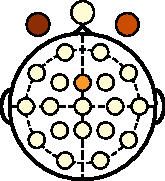
\includegraphics[width=0.17\textwidth]{./img_art_dfa/prop_JGZ_30.pdf} &
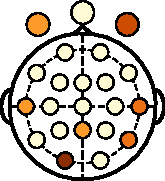
\includegraphics[width=0.17\textwidth]{./img_art_dfa/prop_AEFP_30.pdf} &
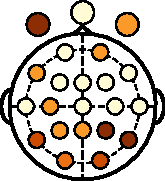
\includegraphics[width=0.17\textwidth]{./img_art_dfa/prop_PCM_30.pdf} \\
\end{tabular}
 \\

\includegraphics[scale=.7]{./img_art_dfa/escala.pdf} \\
\end{tabular}
\caption{Derivaciones para las cuales la proporción de épocas clasificadas como estacionarias fue significativamente diferente en MOR y NMOR.
%
En la parte superior se representa al grupo CTRL y en la parte inferior al grupo PDCL.
%
Para esta figura se usaron épocas de 30 segundos de duración.
%
La posición de los círculos representan a las derivaciones, en correspondencia con la figura \ref{img:estampa}.}
\label{cabeza_new}
\end{figure}

Con base a la hipótesis sobre estacionariedad local, discutida en la sección \ref{sec:est_local}, se procedió a repetir la clasificación de estacionariedad pero usando ventanas de diferentes tamaños.
%
Por fines de comparabilidad y por motivos técnicos, los tamaños de ventana se eligieron de la forma $30 \times 2^{n}$ segundos.
%
El tamaño de ventana más pequeño fue de $\nicefrac{30}{32}$ segundos para poder utilizar la prueba de PSR de forma confiable, mientras que el tamaño más grande fue de $120$ segundos tomando en cuenta que las ventanas más grandes serían demasiado heterogéneos para considerarse como unidades de estudio fiables.

En la figura \ref{cabeza_repoio} se muestra únicamente las proporciones estimadas de épocas estacionarias para MOR y NMOR ($\text{p}_{\text{MOR}}$ y $\text{p}_{\text{NMOR}}$) para un participante; los gráficos construidos para todos los participantes puede encontrarse en el apéndice \ref{apendiceA}.
%
Usando épocas de mayor duración, se encuentra que una proporción menor de estas son clasificadas como estacionarias; sin embargo, usando épocas de menor duración no se garantiza el efecto contrario.
%
Dicho fenómeno \textit{apoya} a la hipótesis de estacionariedad local en los registros de PSG en adultos mayores, aunque no representa evidencia suficiente para relacionarlo con el PDCL.

\begin{figure}
\centering
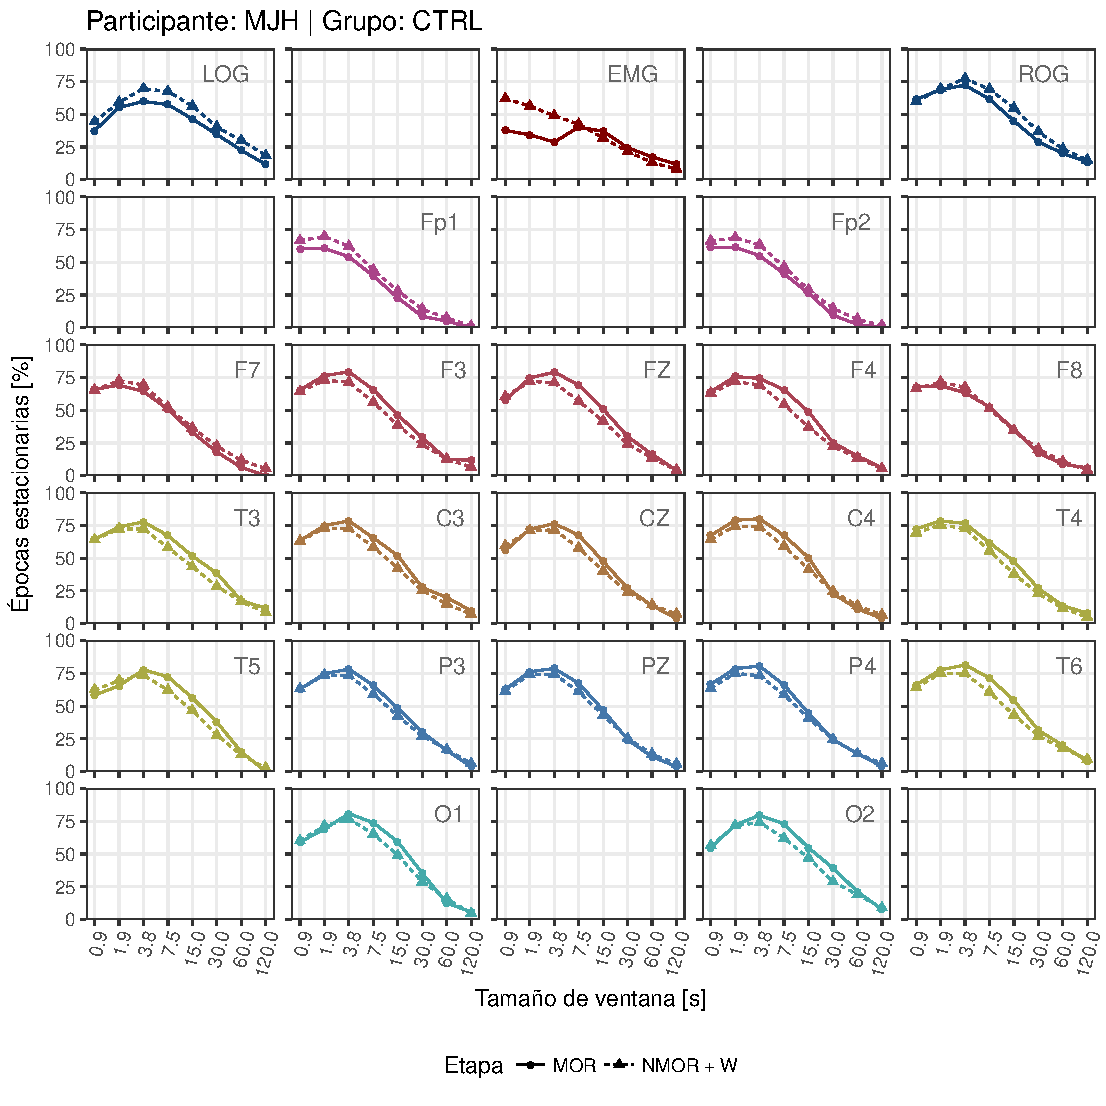
\includegraphics[width=\linewidth]{./scripts_graf_res/MJNNVIGILOS_cabeza_epocas_v2.pdf}
\caption{Cambio en la proporción de épocas estacionarias respecto al tamaño de ventana usado, durante MOR y NMOR. El análisis se repite en todas las derivaciones consideradas; la posición y color de cada gráfico se corresponden a aquellos de la figura \ref{img:estampa}. Sea abrevia W = vigilia, recordando que la cantidad tiempo de los registros clasificada como vigilia es negligible.}
\label{cabeza_repoio}
\end{figure}

En resumen, no se pudo identificar una conexión clara entre el PDCL y las características de las épocas como unidades autónomas.
%
Debido a ello se consideran otros niveles de organización sobre los registros: los registros como un conjunto de épocas distribuidas en el tiempo con \textit{cierta estructura}, y al individuo como unidad en la variabilidad de dichas estructuras.
%
En particular sobre el último, si se supone que las cantidades descritas en esta sección son características \textit{representativas} de cada participante, entonces tiene sentido intentar verificar similitudes con otros participantes o correlaciones con otras observaciones.

%%%%%%%%%%%%%%%%%%%%%%%%%%%%%%%%%%%%%%%%%%%%%%%%%%%%%%%%%%%%%%%%%%%%%%%%%%%%%%%%%%%%%%%%%%%%%%%%%%%
%%%%%%%%%%%%%%%%%%%%%%%%%%%%%%%%%%%%%%%%%%%%%%%%%%%%%%%%%%%%%%%%%%%%%%%%%%%%%%%%%%%%%%%%%%%%%%%%%%%

\section{Análisis a nivel de registro}
\label{sec:analisis_registro}

Como se mencionó en la sección \ref{sec:pdcl_sueno}, se ha reportado cambios en la estructura del sueño en adultos mayores con deterioro cognitivo, respecto a adultos mayores saludables.
%
El objetivo de esta subsección es intentar detectar estos \textit{cambios de estructura} usando los métodos descritos y bajo las condiciones descritas.

Con el fin de explorar cómo se relacionan las épocas estacionarias con la \textit{estructura del sueño}, se procedió a \textit{graficar} la estacionariedad.
%
Para efectuar lo anterior se consideró una cuadrícula, con una fila por cada derivación y una columna por cada época analizada (se registró el mismo número de épocas para cada derivación); sobre la cuadrícula el espacio correspondiente a cada época fue coloreado a según la clasificación de la época como estacionaria.
%
Se procedió similarmente para ilustrar la clasificación según etapa de sueño.
%
En la figura \ref{img:patrones} se ejemplifica este tipo de gráficos, además de otros detalles a mencionarse.

\begin{figure}
\centering
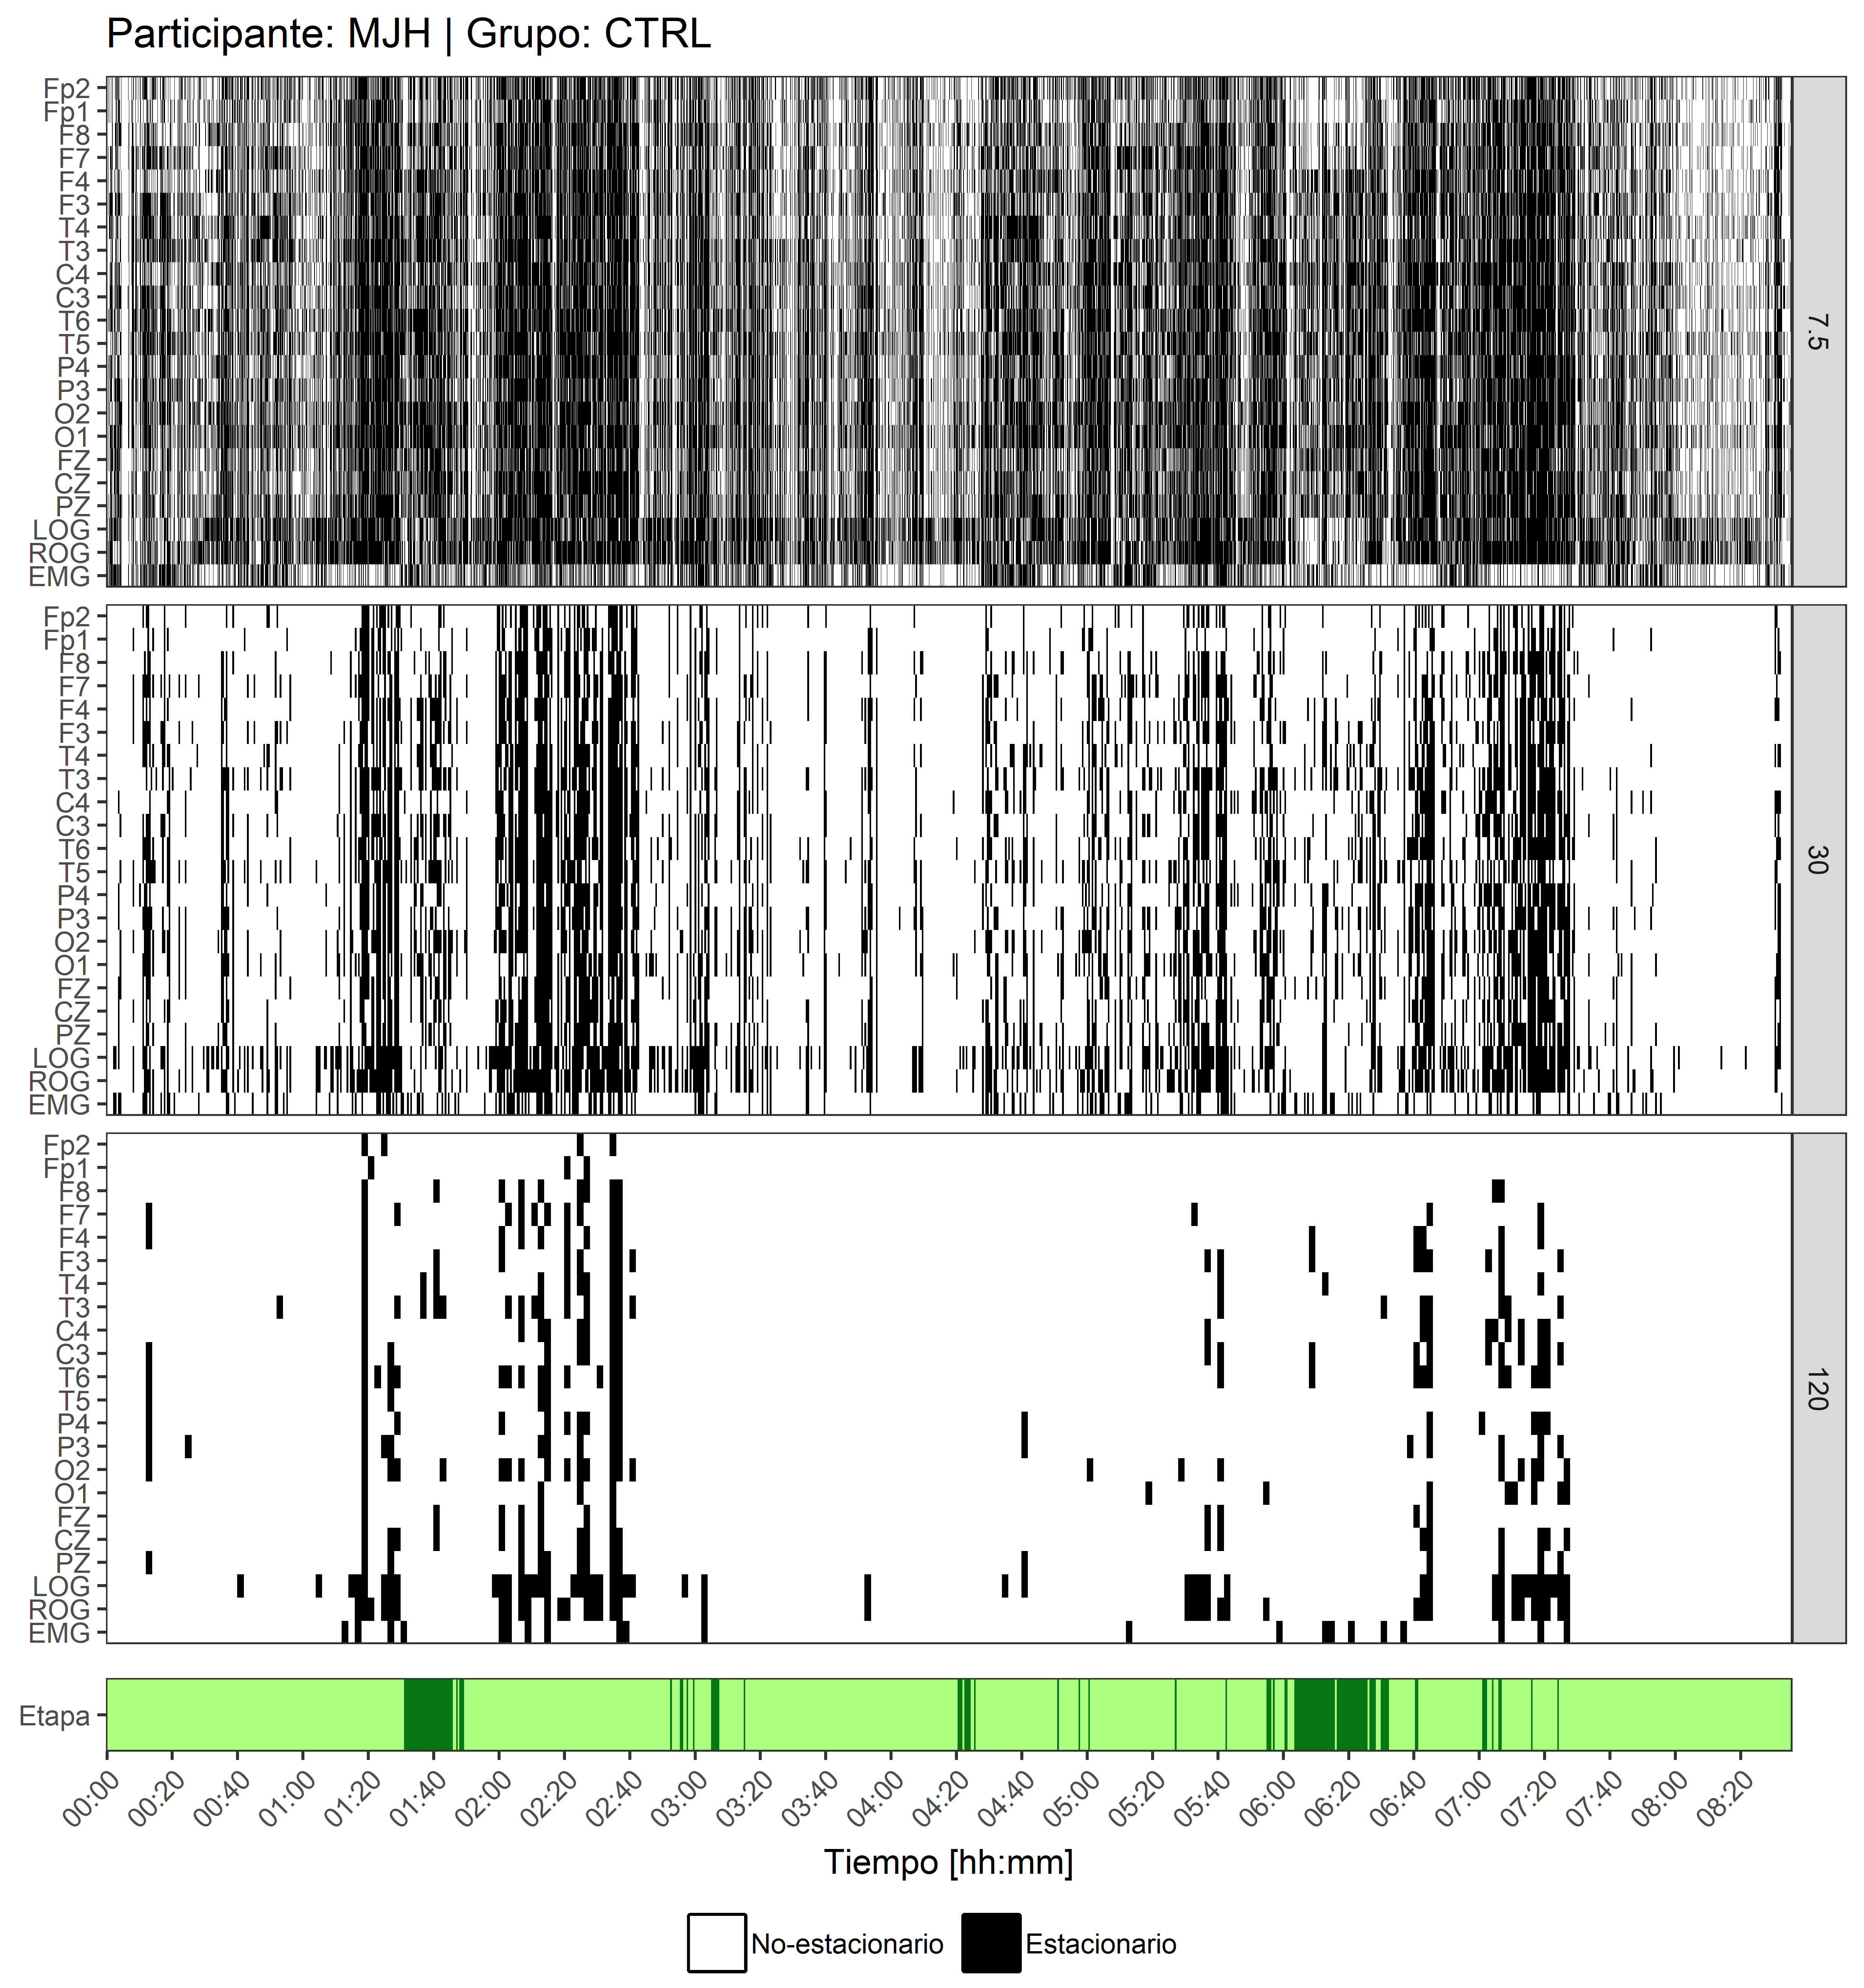
\includegraphics[width=\linewidth]
{./scripts_graf_res/MJNNVIGILOS_patrones_show.png}
\caption[Distribución en el tiempo de las ventanas clasificadas como estacionarias, considerando diferentes tamaños de ventana]{Distribución en el tiempo de las ventanas clasificadas como estacionarias, considerando diferentes tamaños de ventana. 
Cada ventana fue representada en una cuadrícula según su derivación (margen izquierdo) y momento (margen inferior) de procedencia; posteriormente fue \textit{coloreada} según su clasificación como estacionaria.
Dado que la clasificación de estacionariedad se repitió usando diversos tamaños de ventana, éstos se indican en el margen derecho.
En la parte inferior se representan las mismas épocas en su clasificación según etapa de sueño.
%Adicionalmente, en la parte superior se indican los \textit{patrones emergentes} de estacionariedad; para más detalles al respecto, ver el texto.
}
\label{img:patrones}
\end{figure}

Los gráficos obtenidos mediante este procedimiento mostraron algunas regularidades que merecen especial atención: \textit{bloques emergentes} de épocas que comparten clasificación como estacionarias (o como no--estacionarias).
%
Estos bloques identificados visualmente se extienden entre diversas derivaciones; puede verse un ejemplo de ello en la figura \ref{img:patrones}.
%
Debido a la forma en que se efectuó la clasificación de estacionariedad (usando la prueba de PSR) puede garantizarse que estos patrones emergentes no son producidos por la clasificación per se.
%
Se hipotetiza que estos \textit{patrones de estacionariedad}
corresponden a las diferentes etapas de sueño.
%
Posteriormente se discutirá con más detalle al respecto.

El procedimiento de graficación se repitió para las clasificaciones de estacionariedad obtenidas usando diferentes tamaños de ventana, con el fin de verificar si la presencia de los bloques podría atribuirse al tamaño de ventana usado.
%
Se encontró que los patrones aparecen con mayor o menor \textit{nitidez} en los gráficos obtenidos usando diferentes tamaños de ventana, tal como se ilustra en la figura \ref{img:patrones}.

%\begin{figure}
%\centering
%\includegraphics[width=.9\textwidth]
%{./img_art_dfa/zoom_noVCR_v2.png} \\
%\includegraphics[width=.9\textwidth]
%{./img_art_dfa/zoom_siVCR_v2.png}
%\caption[Ubicación de épocas estacionarias en el tiempo y patrones emergentes]
%{Ubicación de épocas estacionarias en el tiempo y patrones emergentes. \textbf{Arriba:} 
%Ubicación de épocas estacionarias en el tiempo.
%\textbf{Abajo:} Patrón de bloques relacionado con el sueño MOR}
%\label{patroncito}
%\end{figure}

%Usando la clasificación de épocas estacionarias, obtenida para diferentes tamaños de ventana, se 
%construyeron más gráficos sobre la ubicación de épocas estacionarias en el tiempo. Estos nuevos
%gráficos, como el de la figura \ref{comp_VCR}, refuerzan heurísticamente la hipótesis de que los 
%patrones son significativos fisiológicamente. 

%Entonces, se propone que los registros de PSG se comportan como procesos localmente estacionarios; 
%más aún, se propone que esta característica cambia cualitativamente en adultos mayores con PDC,
%para los cuales el \textit{nivel de homogeneidad} del PSG es muy similar durante MOR y NMOR.

%\begin{figure}
%\centering
%\includegraphics[width=\linewidth]
%{./img_art_dfa/VCNNS1_comp_est_.png}
%\caption{Distribución en el tiempo de ventanas estacionarias, usando diferentes tamaños
%de ventana.}
%\label{comp_VCR}
%\end{figure}

Dentro del contexto del PDCL en adultos mayores, estos patrones de estacionariedad no serán definidos formalmente ni estudiados detalladamente; se presentan como un hallazgo incidental y como verificación empírica de las capacidades de la técnica descrita para distinguir características que varían en el tiempo.
%
Esta decisión fue tomada considerando la naturaleza fuertemente cualitativa de dichos patrones.

%%%%%%%%%%%%%%%%%%%%%%%%%%%%%%%%%%%%%%%%%%%%%%%%%%%%%%%%%%%%%%%%%%%%%%%%%%%%%%%%%%%%%%%%%%%%%%%%%%%

\section{Análisis a nivel de grupo}

Para fines de esta subsección, se ha supuesto que las proporciones de épocas estacionarias durante MOR y NMOR ($\text{p}_{\text{MOR}}$ y $\text{p}_{\text{NMOR}}$) son características intrínsecas de cada individuo. 
%
En otras palabras, si se repite el registro de PSG para el mismo individuo y bajo condiciones similares, y se realiza el mismo procedimiento de segmentación y clasificación de épocas, entonces se espera que las cantidades $\text{p}_{\text{MOR}}$ y $\text{p}_{\text{NMOR}}$ serán las mismas.
%
Este supuesto se basa en que las fases de sueño son \textit{casi indistinguibles} entre diferentes individuos con características similares, y más aún entre diferentes jornadas de sueño para el mismo individuo.
%; para un estudio más detallado de estas últimas afirmaciones, consultar el libro \textit{``Psicofisiología del sueño"} \cite{Corsi1983}.

Con base a los resultados de la subsección anterior, se puede afirmar intuitivamente que la metodología descrita \textit{percibe} parte de algunas fases (o subfases) de sueño, las cuales son comunes entre individuos.
%
Sin embargo, aun si tales observaciones fueran verificadas rigurosamente, el supuesto de que $\text{p}_{\text{MOR}}$ y $\text{p}_{\text{NMOR}}$ son características individuales debería ser verificado por separado.
%
Debido a las limitaciones del presente trabajo --especialmente el tamaño muestral reducido y la limitación de un registro por participante-- el supuesto será usado como tal, y no se verificará debido a la falta de datos.
%
En consecuencia, los resultados en la presente subsección se presentan como \textit{indicios}, con la idea de explorarlos en trabajos futuros.

Entonces bien, las cantidades $\text{p}_{\text{MOR}}$ y $\text{p}_{\text{NMOR}}$, calculadas por separado para todos los participante y todas las derivaciones consideradas, fueron tratados como características que se distribuyen de forma aproximadamente normal sobre las poblaciones que representan los grupos CTRL y PDCL.
%
Se efectuó un ANOVA de dos vías para observar los cambios sobre $\text{p}_{\text{MOR}}$ y $\text{p}_{\text{NMOR}}$ debidos al grupo y la etapa de sueño, cuyos resultados se muestran en el cuadro \ref{tabla:anova_prop}.
%
Se encontró que no hay interacciones significativas entre los factores de etapa y grupo para ninguna derivación; así mismo se encontró que hay diferencias significativas para las derivaciones Fp2, F7, LOG y ROG que pueden ser explicadas por el \textit{efecto} de la etapa se sueño, y de forma similar para las derivaciones LOG y ROG con el efecto de grupo.

Las diferencias para LOG y ROG debido, debidas al efecto de `etapa de sueño', puede explicarse perfectamente por la presencia característica de movimientos oculares rápidos en el sueño MOR; en cierto sentido, este resultado era de esperarse.
%
Las diferencias en Fp2 y F7 requieren una explicación más cautelosa, ya que el efecto es significativo en la región frontal, la cual típicamente es asociada con la toma de decisiones; sin embargo, la \textit{significancia} es débil y no es consistente sobre la región frontal.
%
Para explorar más a fondo los resultados de la ANOVA, en la figura \ref{comparacion_verde} se han graficado (como diagramas de caja) los valores $\text{p}_{\text{MOR}}$ y $\text{p}_{\text{NMOR}}$ muestrales; se observa que intuitivamente las cantidades $\text{p}_{\text{MOR}}$ y $\text{p}_{\text{NMOR}}$ entre grupos y entre etapas, pero no resultan significativas debido a la gran variablidad dentro de las categrorías.
%
En principio es posible justificar dicha falla por una muestra muy pequeña.

Con respecto a las diferencias entre grupos para las derivaciones LOG y ROG, puede decirse que recientemente se ha sugerido que es posible detectar diferencias entre sujetos con y sin DCL usando registros de --entre otras derivaciones-- movimientos oculares [articulo??].

\begin{SidewaysTable}
\centering
\caption{ANOVA para los efectos Grupo y Etapa de sueño sobre las cantidades $\text{p}_{\text{MOR}}$ y $\text{p}_{\text{NMOR}}$.}
\label{tabla:anova_prop}
\begin{tabular}{lllllllllllllrllrllrl}
\toprule
 & \multicolumn{5}{l}{CTRL} &  & \multicolumn{5}{l}{PDCL} &  & \multicolumn{8}{l}{ANOVA} \\
\cmidrule{2-6} \cmidrule{8-12} \cmidrule{14-18}
 & \multicolumn{2}{l}{NMOR} &  & \multicolumn{2}{l}{MOR} &  & \multicolumn{2}{l}{NMOR} &  & \multicolumn{2}{l}{MOR} &  & \multicolumn{2}{l}{Grupo} &  & \multicolumn{2}{l}{Etapa} &  & \multicolumn{2}{l}{G$\times$E} \\
\cmidrule{2-3} \cmidrule{5-6} \cmidrule{8-9} \cmidrule{11-12} \cmidrule{14-15} \cmidrule{17-18} \cmidrule{20-21} 
 & M & DE & & M & DE & & M & DE & & M & DE & & F & p & & F & p & & F & p \\
\midrule
Fp2 & .172 & .040 &  & .063 & .058 &  & .106 & .084 &  & .037 & .070 &  & 2.08 & .171 &  & 7.51 & .016 &  & .40 & .537 \\
Fp1 & .175 & .090 &  & .091 & .115 &  & .108 & .105 &  & .045 & .077 &  & 1.53 & .237 &  & 2.48 & .138 &  & .05 & .829 \\
F8 & .193 & .076 &  & .147 & .133 &  & .125 & .078 &  & .089 & .140 &  & 1.43 & .252 &  & .60 & .453 &  & .01 & .918 \\
F7 & .190 & .050 &  & .077 & .076 &  & .126 & .096 &  & .055 & .106 &  & 1.09 & .314 &  & 4.81 & .046 &  & .25 & .621 \\
F4 & .200 & .055 &  & .162 & .145 &  & .144 & .125 &  & .152 & .151 &  & .30 & .595 &  & .04 & .836 &  & .14 & .716 \\
F3 & .199 & .040 &  & .144 & .099 &  & .151 & .138 &  & .171 & .230 &  & .02 & .890 &  & .03 & .858 &  & .27 & .610 \\
T4 & .224 & .076 &  & .212 & .171 &  & .162 & .078 &  & .262 & .190 &  & .01 & .926 &  & .57 & .461 &  & .71 & .414 \\
T3 & .272 & .066 &  & .281 & .148 &  & .187 & .095 &  & .245 & .207 &  & .79 & .390 &  & .28 & .603 &  & .13 & .726 \\
C4 & .294 & .079 &  & .232 & .159 &  & .169 & .124 &  & .256 & .188 &  & .53 & .481 &  & .09 & .772 &  & 1.15 & .301 \\
C3 & .255 & .054 &  & .248 & .115 &  & .188 & .122 &  & .250 & .180 &  & .28 & .604 &  & .27 & .614 &  & .31 & .585 \\
T6 & .315 & .105 &  & .241 & .151 &  & .170 & .093 &  & .250 & .210 &  & .94 & .349 &  & .03 & .871 &  & 1.20 & .292 \\
T5 & .294 & .167 &  & .337 & .231 &  & .222 & .149 &  & .320 & .178 &  & .27 & .612 &  & .74 & .403 &  & .10 & .755 \\
P4 & .258 & .060 &  & .201 & .134 &  & .158 & .100 &  & .227 & .194 &  & .33 & .576 &  & .04 & .843 &  & .95 & .345 \\
P3 & .256 & .097 &  & .227 & .138 &  & .187 & .101 &  & .286 & .190 &  & .01 & .939 &  & .42 & .526 &  & .93 & .350 \\
O2 & .272 & .078 &  & .243 & .181 &  & .183 & .112 &  & .255 & .210 &  & .26 & .615 &  & .13 & .721 &  & .47 & .506 \\
O1 & .278 & .095 &  & .291 & .209 &  & .175 & .117 &  & .253 & .206 &  & .81 & .383 &  & .40 & .539 &  & .17 & .685 \\
FZ & .234 & .031 &  & .242 & .109 &  & .168 & .139 &  & .215 & .178 &  & .55 & .469 &  & .24 & .634 &  & .10 & .758 \\
CZ & .225 & .062 &  & .187 & .111 &  & .164 & .120 &  & .178 & .127 &  & .46 & .510 &  & .03 & .865 &  & .24 & .633 \\
PZ & .229 & .049 &  & .176 & .100 &  & .160 & .119 &  & .230 & .177 &  & .02 & .904 &  & .07 & .797 &  & 1.06 & .321 \\
LOG & .505 & .103 &  & .229 & .132 &  & .343 & .089 &  & .094 & .096 &  & 9.10 & .009 &  & 28.19 & .000 &  & .08 & .786 \\
ROG & .542 & .149 &  & .305 & .173 &  & .342 & .171 &  & .143 & .133 &  & 5.89 & .029 &  & 8.53 & .011 &  & .07 & .800 \\
EMG & .151 & .082 &  & .162 & .094 &  & .068 & .074 &  & .139 & .166 &  & .99 & .337 &  & .68 & .423 &  & .31 & .588 \\
\bottomrule 
\multicolumn{20}{l}{M=media muestral; SD=Desviación estándar; G$\times$E=interacción Grupo y Etapa}
\end{tabular}
\end{SidewaysTable}

\begin{figure}
\centering
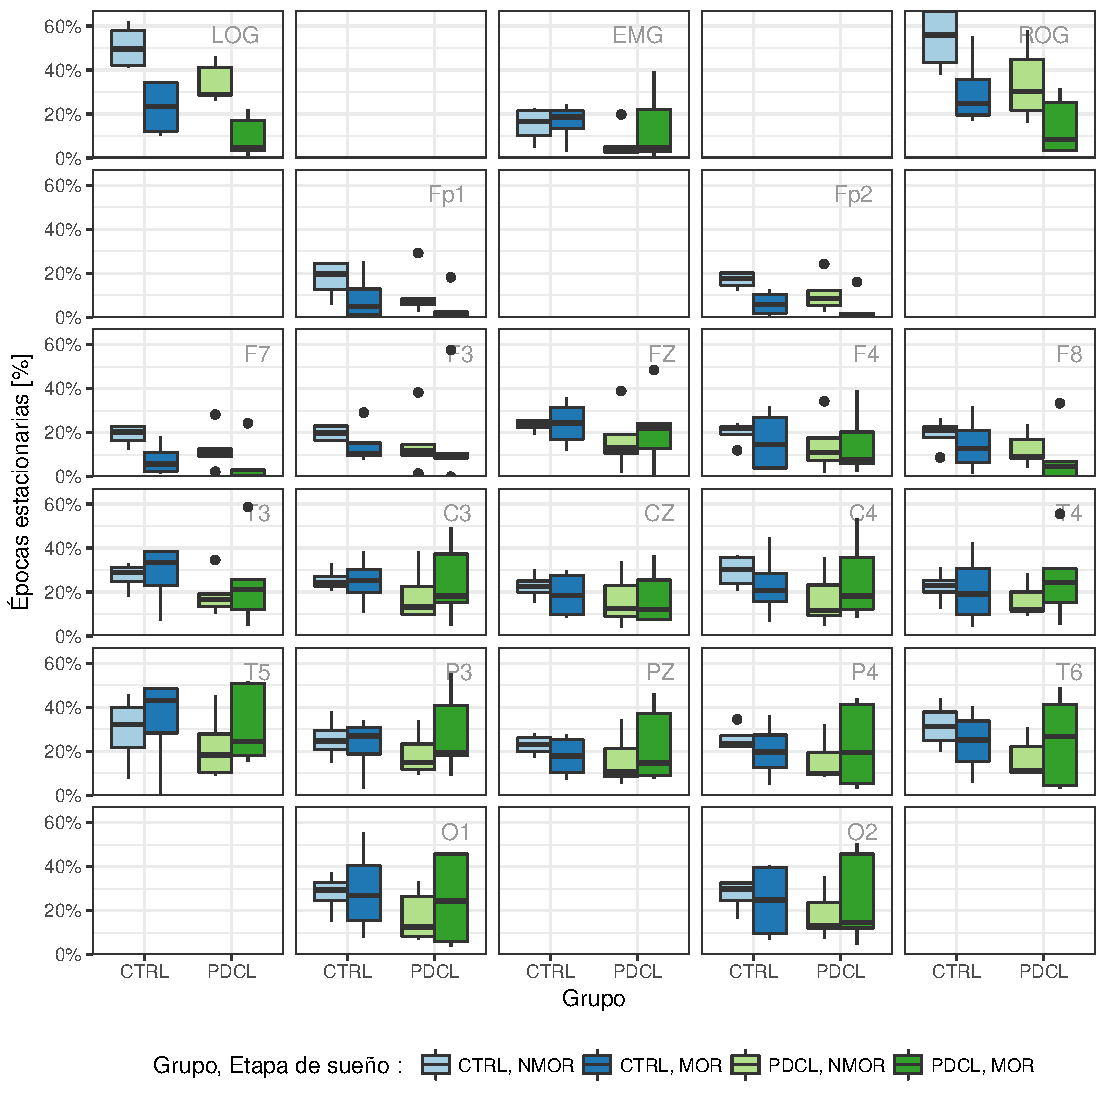
\includegraphics[width=\linewidth]
{./scripts_graf_res/comparacion_cabeza.pdf}
\caption{Proporciones de épocas estacionarias, durante sueño MOR y NMOR y para todas las derivaciones.
%
Los puntos representan valores \textit{atípicos}, según su definición para diagramas de caja (ver sección ??).
%; es decir, aquellos valores fuera del intervalo $[Q_1-1.5 R, Q_3 + 1.5 R]$, con $Q_1$ y $Q_3$ el primero y tercer cuartiles muestrales y $R=Q_3-Q_1$.
%
La posición de cada gráfico se corresponden con aquellos de la figura \ref{img:estampa}.}
\label{comparacion_verde}
\end{figure}

%\begin{figure}
%\centering
%\includegraphics[width=\linewidth]
%{./img_art_dfa/Comparacion_gpos_CTL_PDC_v3.pdf}
%\caption{Proporciones de épocas estacionarias, durante sueño MOR y NMOR.}
%\label{comparacion_verde}
%\end{figure}
%
%\begin{figure}
%\centering
%\includegraphics[width=\linewidth]
%{./img_art_dfa/Comparacion_gpos_MOR_NMOR_v3.pdf}
%\caption{Proporciones de épocas estacionarias, grupos CTL y PDC.}
%\label{comparacion_graf}
%\end{figure}

%%%%%%%%%%%%%%%%%%%%%%%%%%%%%%%%%%%%%%%%%%%%%%%%%%%%%%%%%%%%%%%%%%%%%%%%%%%%%%%%%%%%%%%%%%%%%%%%%%%
%%%%%%%%%%%%%%%%%%%%%%%%%%%%%%%%%%%%%%%%%%%%%%%%%%%%%%%%%%%%%%%%%%%%%%%%%%%%%%%%%%%%%%%%%%%%%%%%%%%
%%%%%%%%%%%%%%%%%%%%%%%%%%%%%%%%%%%%%%%%%%%%%%%%%%%%%%%%%%%%%%%%%%%%%%%%%%%%%%%%%%%%%%%%%%%%%%%%%%%

%%%%%%%%%%%%%%%%%%%%%%%%%%%%%%%%%%%%%%%%%%%%%%%%%%%%%%%%%%%%%%%%%%%%%%%%%%%%%%%%%%%%%%%%%%%%%%%%%%%
%%%%%%%%%%%%%%%%%%%%%%%%%%%%%%%%%%%%%%%%%%%%%%%%%%%%%%%%%%%%%%%%%%%%%%%%%%%%%%%%%%%%%%%%%%%%%%%%%%%
%%%%%%%%%%%%%%%%%%%%%%%%%%%%%%%%%%%%%%%%%%%%%%%%%%%%%%%%%%%%%%%%%%%%%%%%%%%%%%%%%%%%%%%%%%%%%%%%%%%

\section{Aplicación de la prueba de Priestley-Subba Rao}

Se fragmentaron los registros en ventanas de 30 segundos de duración, sin traslape. Cada una de 
estas ventanas fue sometida a la prueba de PSR, y se clasificó como \textit{estacionaria en el 
sentido de PSR} si fue posible rechazar ($p<0.05$) la hipótesis de no-estacionariedad. 
%
Los resultados obtenidos (una lista de las épocas que son estacionarias) se guardaron en archivos 
de texto para su posterior análisis. 
%
Debido a la gran variabilidad entre el tiempo que los participantes pasaron en sueño MOR, se decidió
basar las comparaciones en proporciones de épocas; por ejemplo, se calculó la proporción de
épocas MOR que son estacionarias para todos los participantes.

%\begin{figure}
%\centering
%\begin{lstlisting}[caption={}]
%Priestley-Subba Rao stationarity Test for datos
%-----------------------------------------------
%Samples used              : 3072 
%Samples available         : 3069 
%Sampling interval         : 1 
%SDF estimator             : Multitaper 
%  Number of (sine) tapers : 5 
%  Centered                : TRUE 
%  Recentered              : FALSE 
%Number of blocks          : 11 
%Block size                : 279 
%Number of blocks          : 11 
%p-value for T             : 0.4130131 
%p-value for I+R           : 0.1787949 
%p-value for T+I+R         : 0.1801353 
%\end{lstlisting}
%\caption[Resultado típico para la función \texttt{stationarity}]
%{Resultado típico para la función \texttt{stationarity}. La función de densidad espectral es
%referida como SDF, mientras que los p valores. El p-valor para \texttt{T+I+R} corresponde al 
%estadístico $S_{I+R}$, y el p-valor para \texttt{T} corresponde $S_T$
%}
%\label{res_psr}
%\end{figure}

Como análisis exploratorio se graficaron en el tiempo las épocas, en todos los canales, como se 
muestra en la figura \ref{patroncito}. Este tipo de gráficos \textit{revelan} cierto tipo de 
\textit{bloques} de épocas estacionarias o no-estacionarias. Heurísticamente se puede afirmar que 
éstos patrones son independientes de la prueba de PSR, y anteriormente se reportó que estos patrones
suelen coincidir con la aparición de sueño MOR. Más adelante se ofrece una discusión al 
respecto.

\begin{figure}
\centering
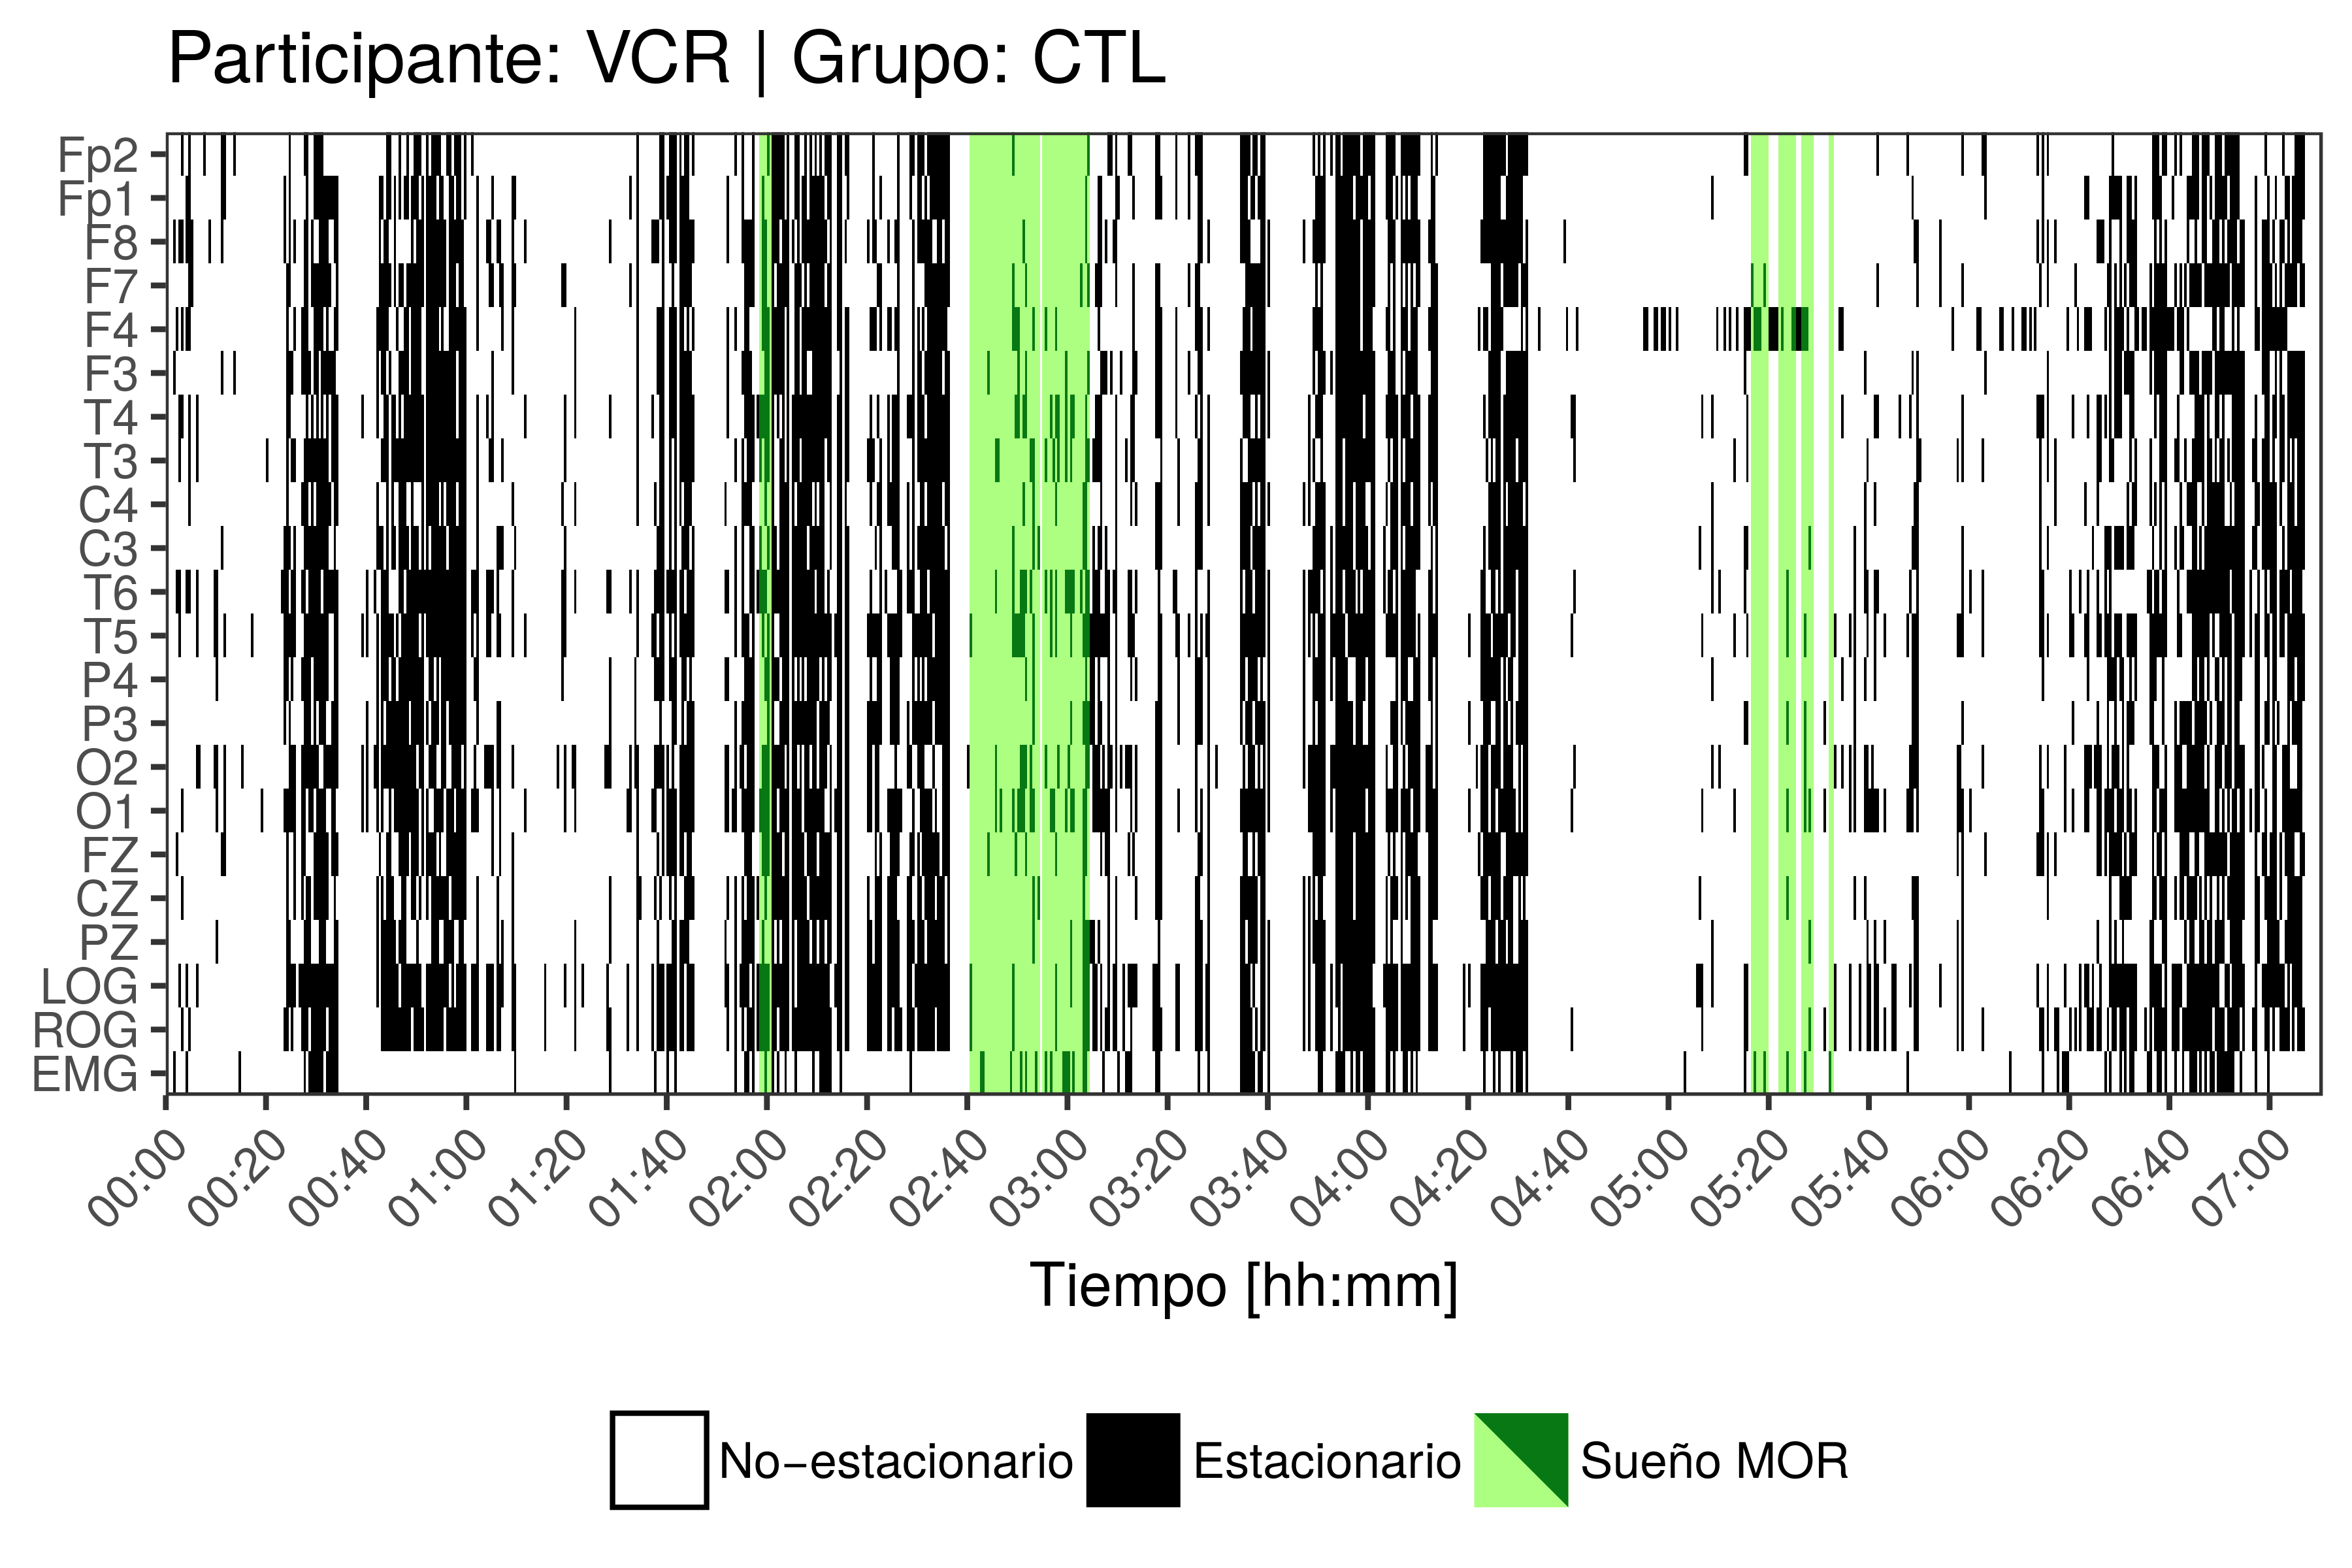
\includegraphics[width=.9\textwidth]
{./img_art_dfa/zoom_noVCR_v2.png} \\
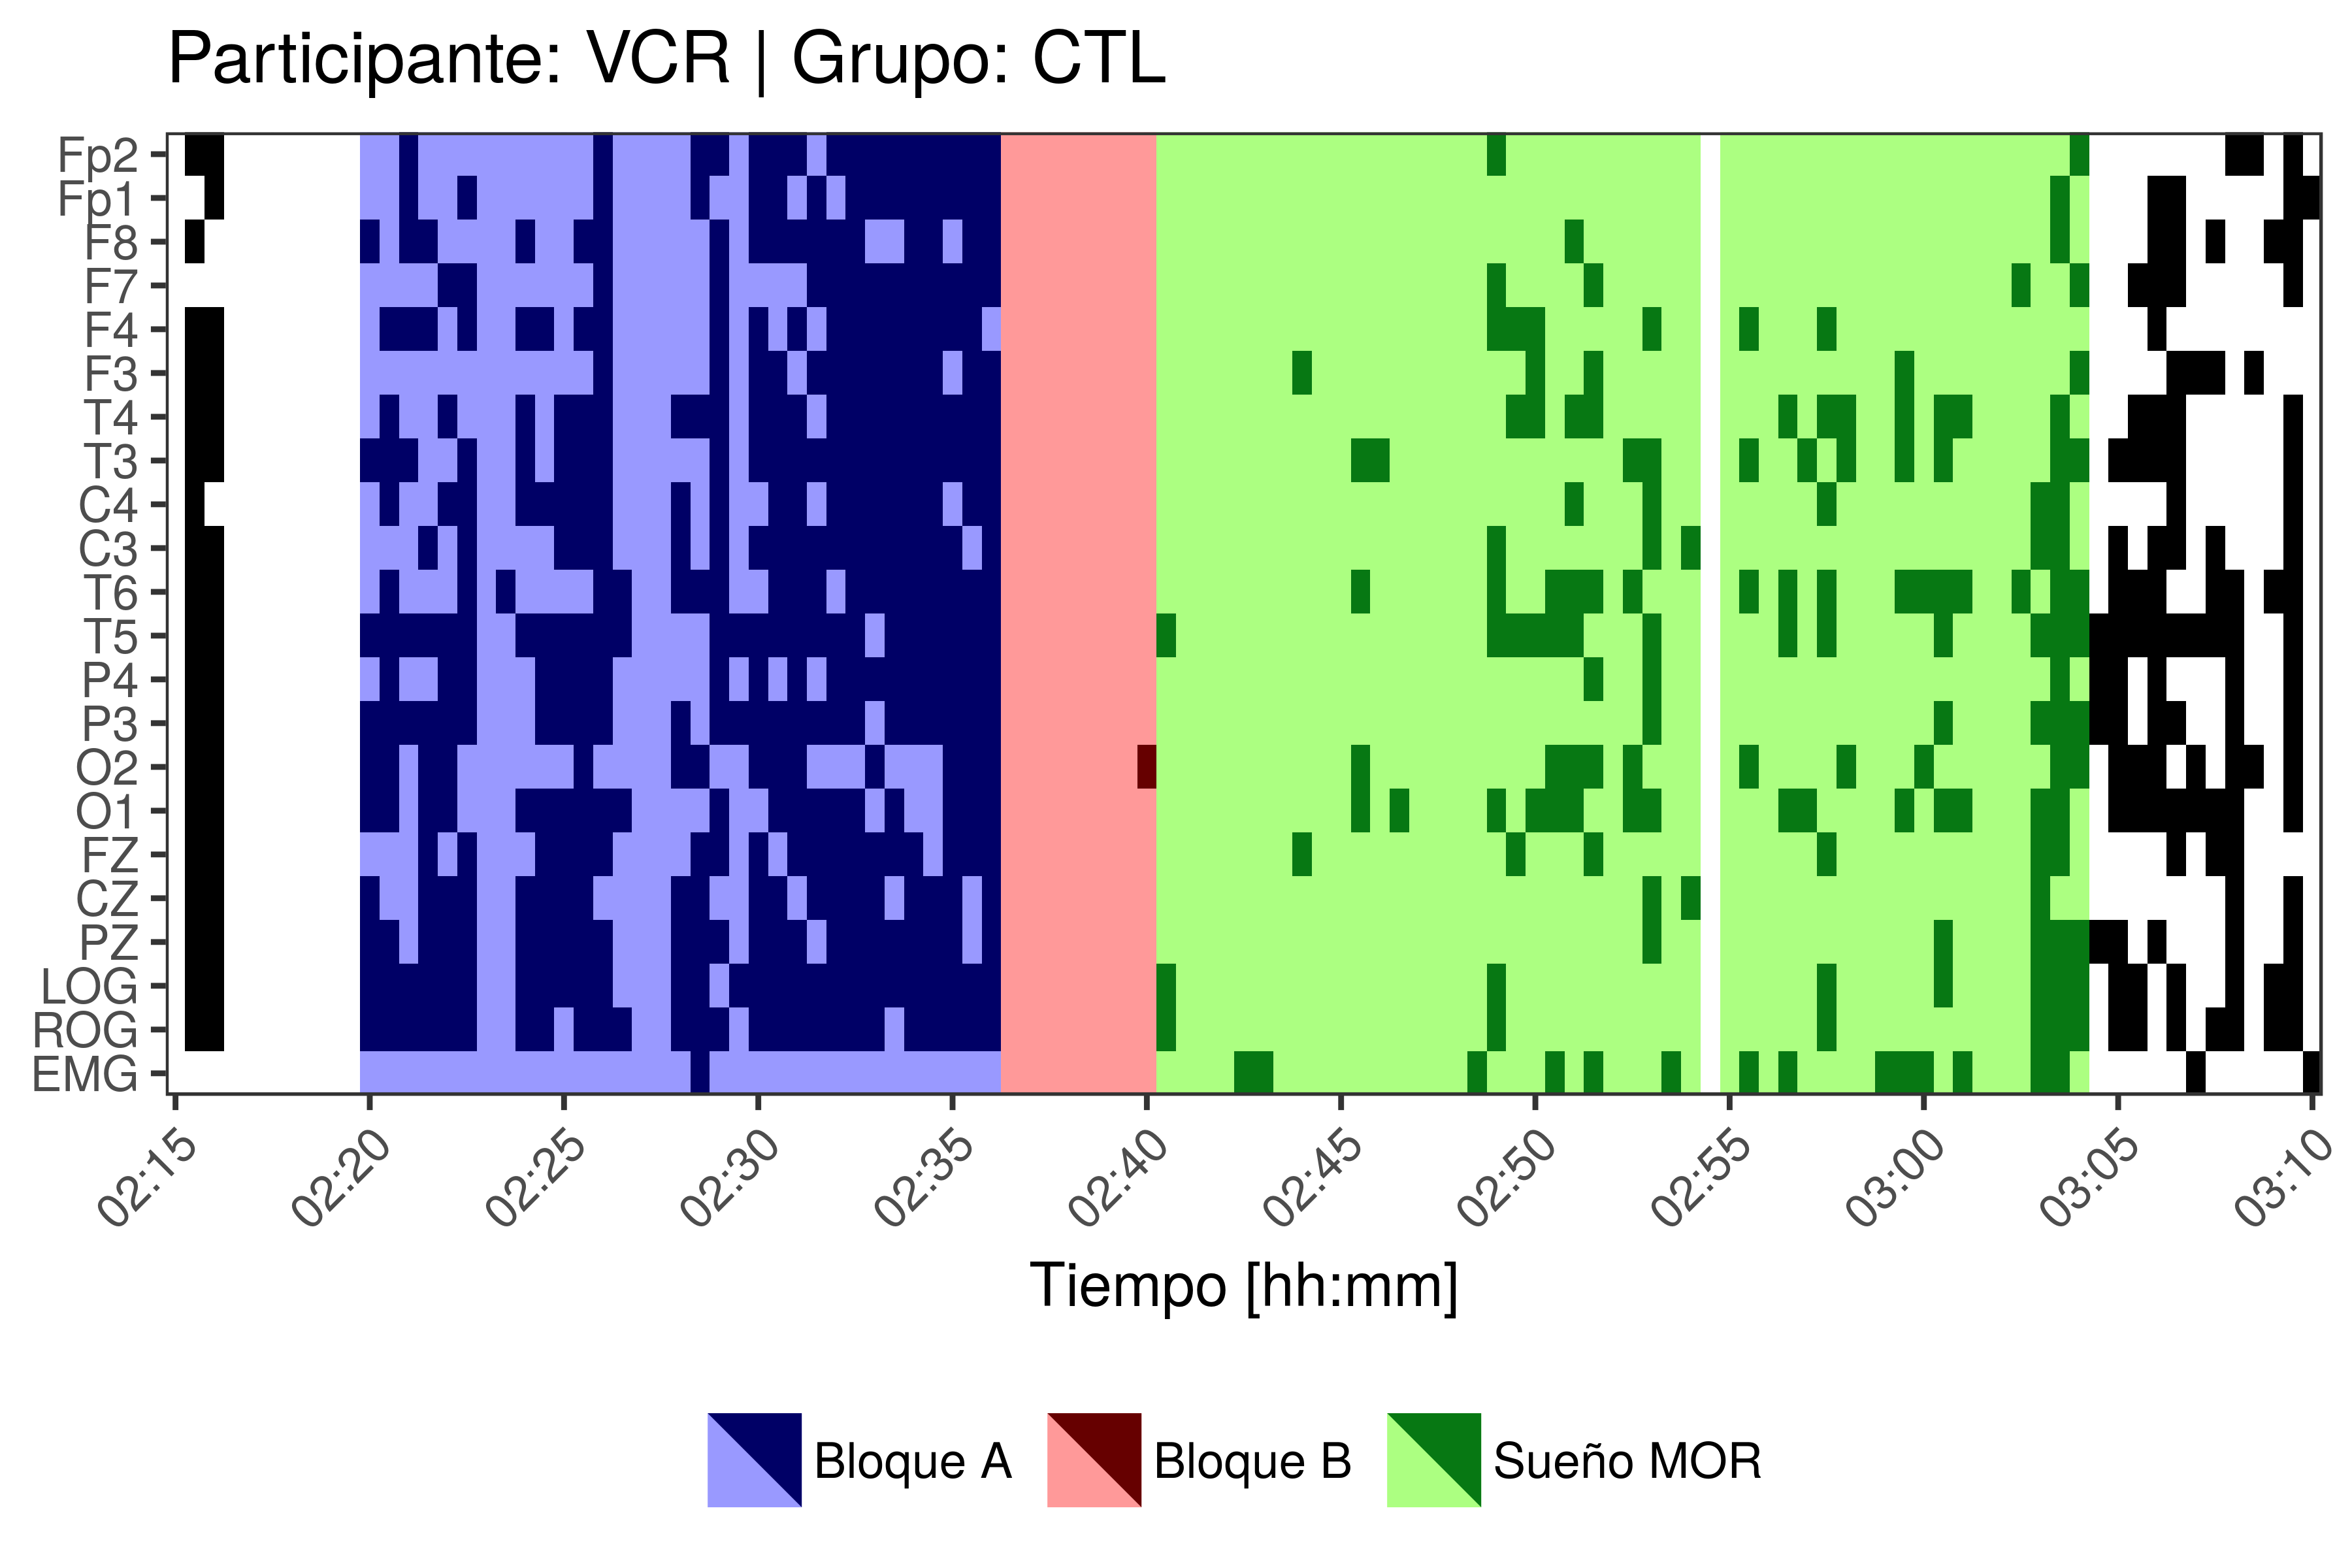
\includegraphics[width=.9\textwidth]
{./img_art_dfa/zoom_siVCR_v2.png}
\caption[Ubicación de épocas estacionarias en el tiempo y patrones emergentes]
{Ubicación de épocas estacionarias en el tiempo y patrones emergentes. \textbf{Arriba:} 
Ubicación de épocas estacionarias en el tiempo.
\textbf{Abajo:} Patrón de bloques relacionado con el sueño MOR}
\label{patroncito}
\end{figure}

En otro ámbito, se replicó la metodología usada por McEwen \cite{McEwen75} para contrastar la 
afirmación de que las series de tiempo \textit{suficiente cortas} son estacionarias. 
%
Este procedimiento consistió en repetir la clasificación de épocas variando el tamaño de ventana; 
los tamaños de ventana se tomaron de la forma $30 \times 2^{n}$ segundos, para comparar con el 
tamaño de época recomendado por la AASM.

Usando la clasificación de épocas estacionarias, obtenida para diferentes tamaños de ventana, se 
construyeron más gráficos sobre la ubicación de épocas estacionarias en el tiempo. Estos nuevos
gráficos, como el de la figura \ref{comp_VCR}, refuerzan heurísticamente la hipótesis de que los 
patrones son significativos fisiológicamente. 

En base a resultados previos usando esta técnica, se espera que el comportamiento de los patrones 
visuales obedezca al fenómeno de \textbf{estacionariedad local}; esta característica, descrita por 
Dahlhaus \cite{Dahlhaus97}, implica que un proceso puede ser aproximado a trozos 
\textit{ensamblando} procesos estacionarios.
%
Esta caracterización del EEG ha sido usada anteriormente de manera fructífera pero problemática
\cite{Barlow85,Kaplan99}.
%
Dentro del modelo para registros de PSG, la estacionariedad local significa que el PSG no es
formalmente homogéneo \textit{pero} puede entenderse como varios segmentos homógeneos. En un
sentido más general, es coherente pensar que el PSG se componga tanto de segmentos homógeneos
como de \textit{eventos puntuales} y artefactos.

En la figura \ref{epocas_diferentes} se muestra esquemáticamente cómo el tamaño
de las ventanas puede influir para su clasificación como estacionarias/homogéneas.

Entonces, se propone que los registros de PSG se comportan como procesos localmente estacionarios; 
más aún, se propone que esta característica cambia cualitativamente en adultos mayores con PDC,
para los cuales el \textit{nivel de homogeneidad} del PSG es muy similar durante MOR y NMOR.

\begin{figure}
\centering
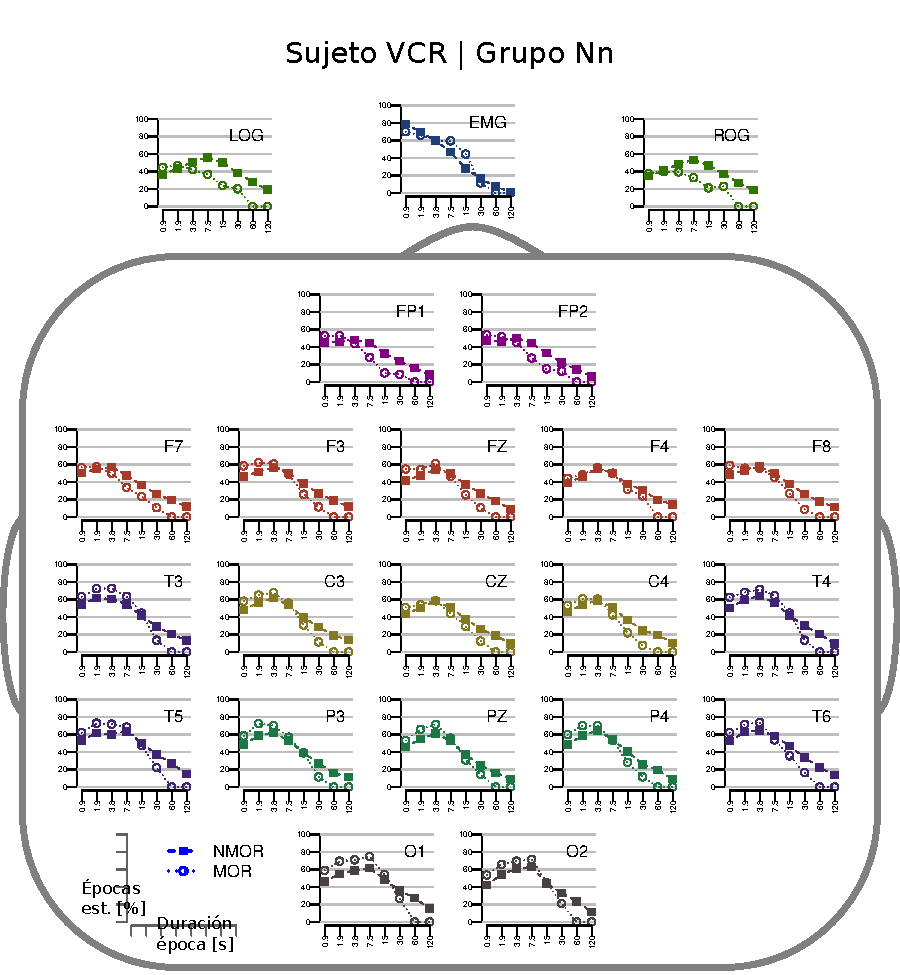
\includegraphics[width=.9\linewidth]{./img_resultados/cabeza_VCR.pdf}
\caption{Cambio en el porcentaje de épocas estacionarias conforme el tamaño de ventana}
\label{cabeza_repoio}
\end{figure}

\begin{figure}
\centering
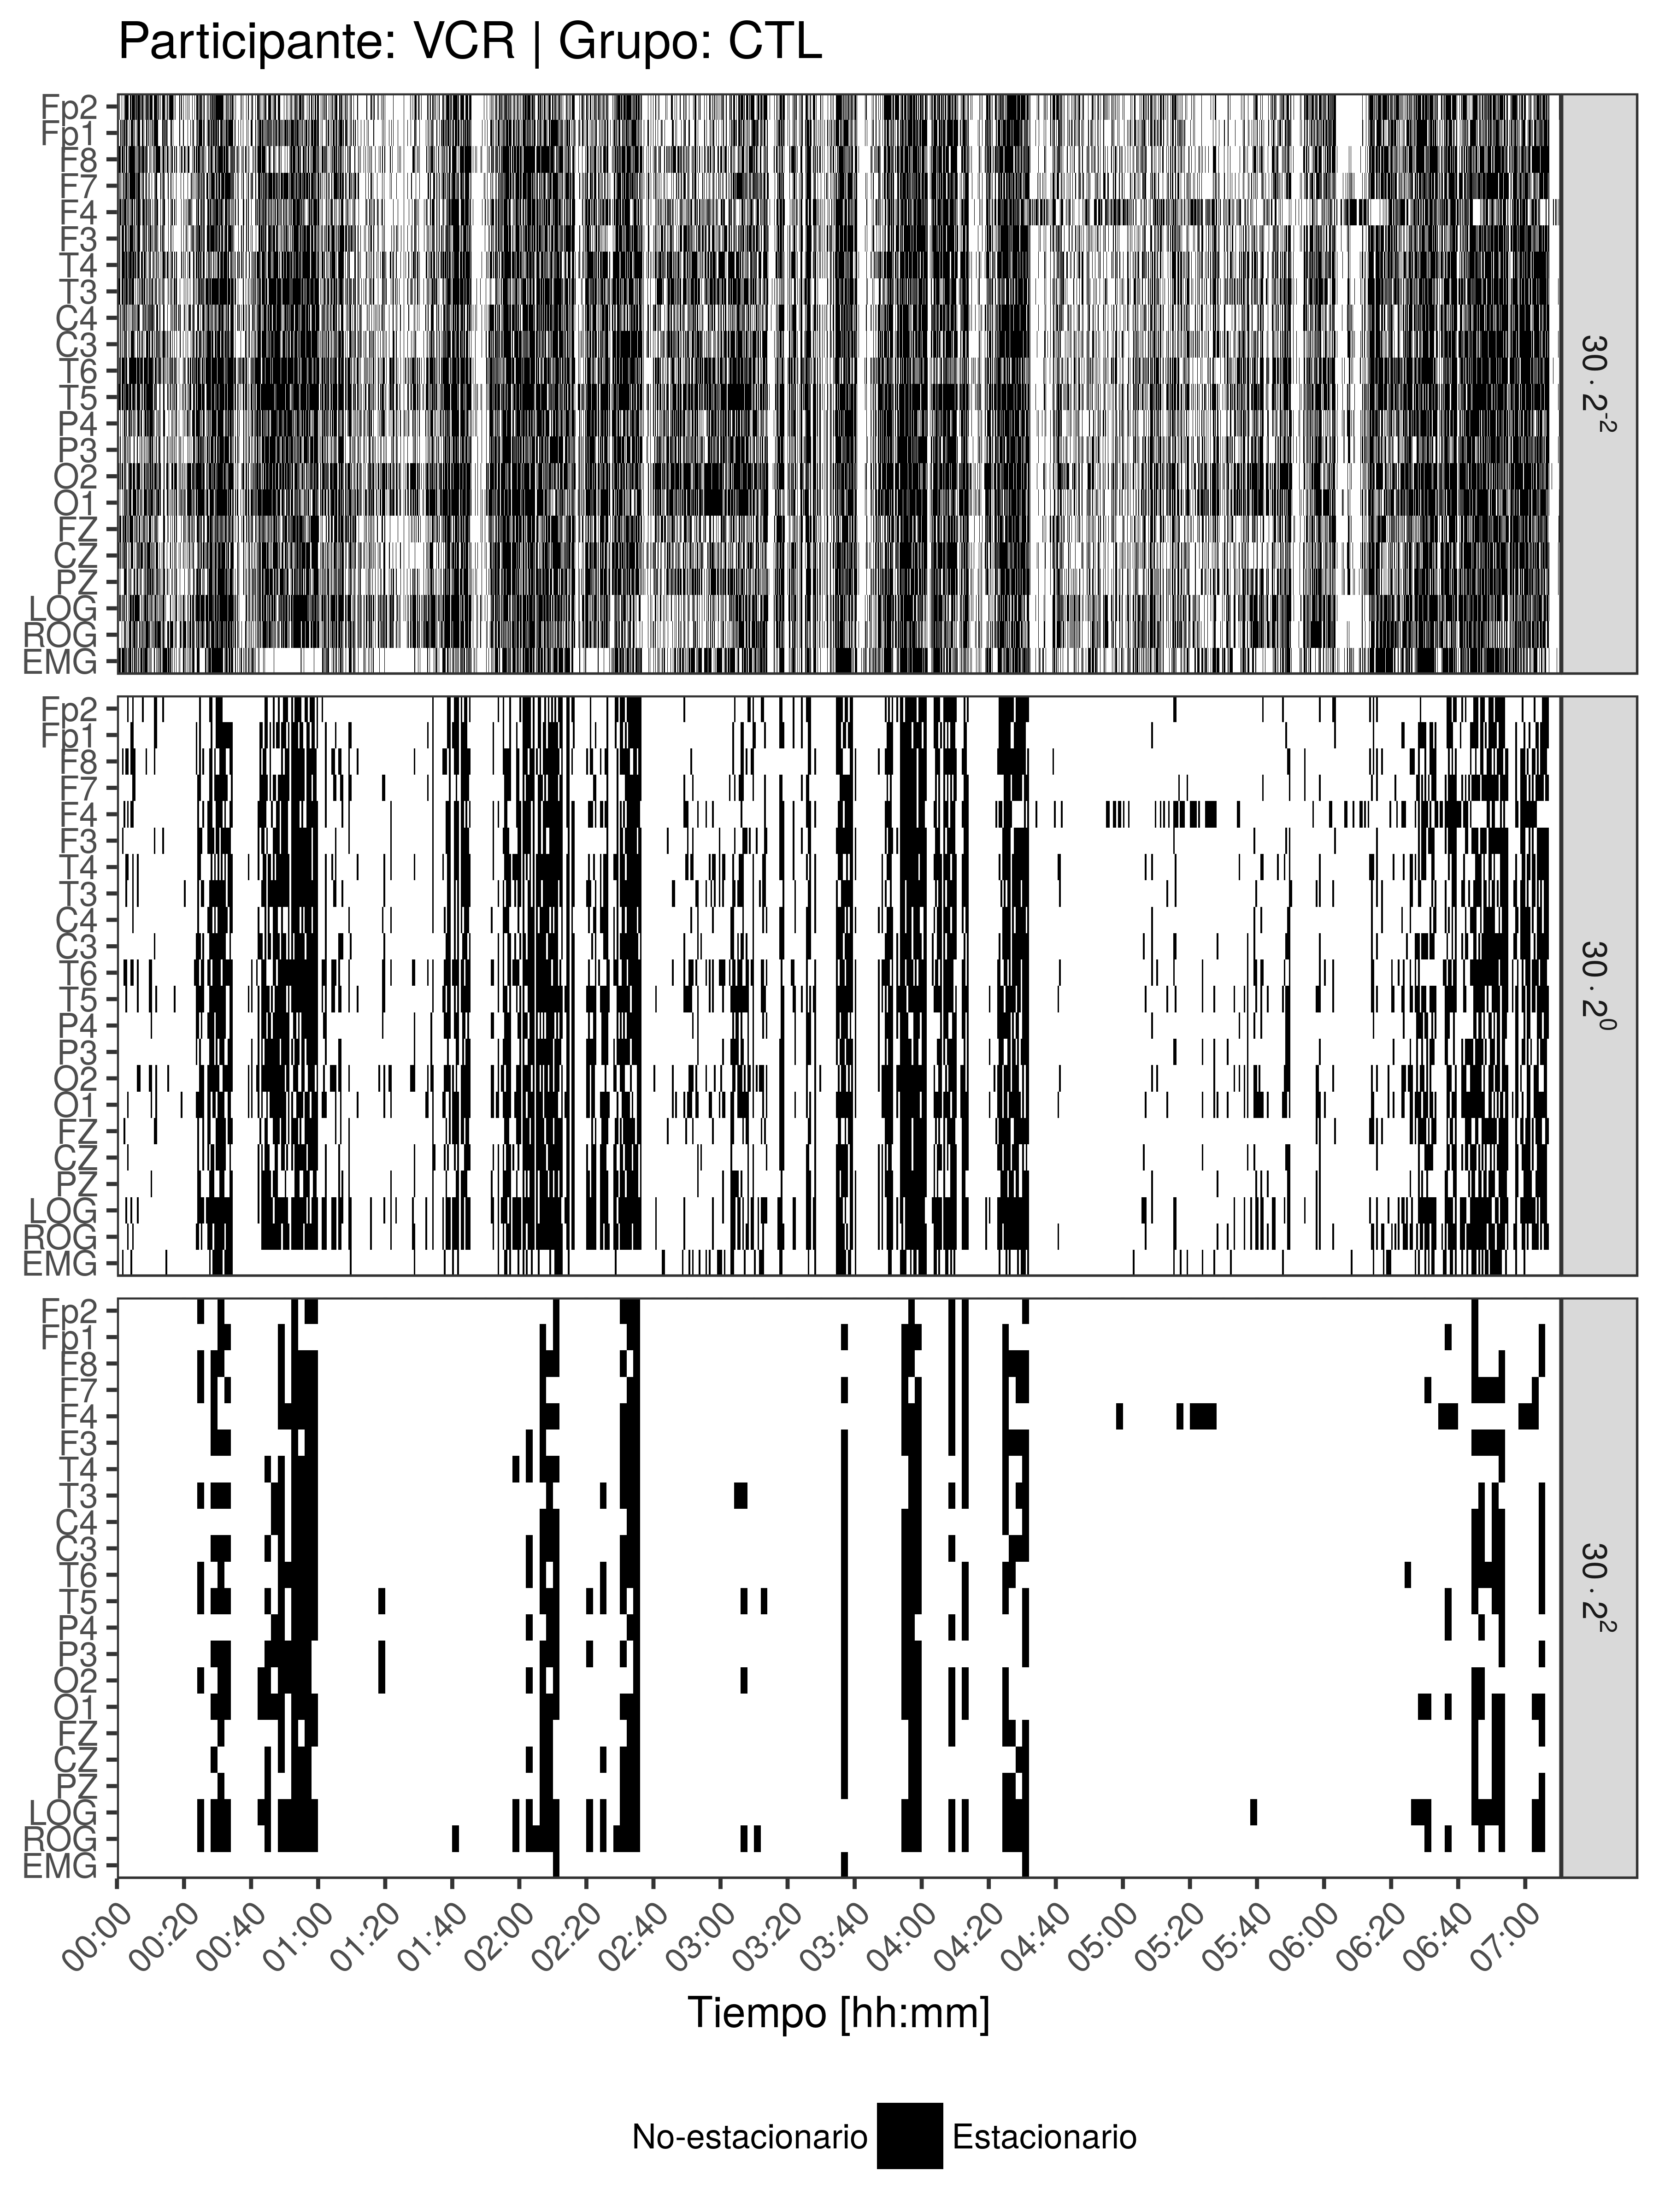
\includegraphics[width=\linewidth]
{./img_art_dfa/VCNNS1_comp_est_.png}
\caption{Distribución en el tiempo de ventanas estacionarias, usando diferentes tamaños
de ventana.}
\label{comp_VCR}
\end{figure}

Cabe destacar que la aplicación \textit{per se} de la prueba fue efectuada usando el software 
estadístico R \cite{R_citar}. En particular, se utilizó la implementación 
incluida en el paquete \texttt{fractal} \cite{R_fractal} bajo la función \texttt{stationarity}.

%%%%%%%%%%%%%%%%%%%%%%%%%%%%%%%%%%%%%%%%%%%%%%%%%%%%%%%%%%%%%%%%%%%%%%%%%%%%%%%%%%%%%%%%%%%%%%%%%%%
%%%%%%%%%%%%%%%%%%%%%%%%%%%%%%%%%%%%%%%%%%%%%%%%%%%%%%%%%%%%%%%%%%%%%%%%%%%%%%%%%%%%%%%%%%%%%%%%%%%

%\section{Espectro de potencias}
%
%Adicionalmente a la clasificación de épocas como estacionarias, se calculó su espectro de potencia. 
%Como una metodología común, se calculó el \textbf{espectro de banda ancha},
%es decir, la potencia total y relativa correspondientes a las frecuencias que caracterizan las ondas 
%delta, theta, alfa, beta y gamma (ver cuadro \ref{tabla_ondas}).
%
%\begin{figure}
%\centering
%\includegraphics[width=\linewidth]
%{./img_art_dfa/VCNNS1_espectral_total.png} 
%\caption[Espectro de potencias de banda ancha]{Espectro de potencias de banda ancha (delta, theta
%alfa, beta, gamma).}
%\end{figure}
%
%Usando los espectros de banda ancha se ha calculado el coeficiente de enlentecimiento \lento, 
%definido en la 
%expresión \ref{enlentecimiento}, con particular atención al sueño MOR. Esta cantidad
%se ha reportado como un posible marcador de deterioro cognitivo leve en adultos mayores 
%\cite{Brayet16}.
%
%\begin{equation}
%\text{R}_{\text{E}} = \frac{\text{potencia}_{\delta}+\text{potencia}_{\theta}}
%{\text{potencia}_{\alpha}+\text{potencia}_{\beta}} =
%\frac{\int_{\text 0.5 \hz}^{\text{7 \hz}}h(\omega) d\omega}
%{\int_{\text 7 \hz}^{\text{30 \hz}}h(\omega) d\omega}
%\label{enlentecimiento}
%\end{equation}
%
%El espectro de potencias se ha calculado usado el estimador adaptativo propuesto por
%Barbour y Parker \cite{Barbour14}, el cual se encuentra implementado dentro del paquete
%\texttt{psd} bajo la función \texttt{pspectrum}.
%Se ha usado dicho estimador para garantizar heurísticamente que el espectro de potencias
%calculado (1) es independiente del usado para determinar la estacionariedad y (2)
%es compatible con la metodología \textit{usual}; como el algoritmo \texttt{psd} 
%supone estacionariedad débil se espera que emule resultados 
%obtenidos bajo tal supuesto.
%
%Como se discute posteriormente, los bloques de épocas estacionarias están relacionados a bloques
%cuyo espectro de potencia son distintos. Así mismo son diferentes los coeficientes \lento calculados
%para dichos bloques.

%%%%%%%%%%%%%%%%%%%%%%%%%%%%%%%%%%%%%%%%%%%%%%%%%%%%%%%%%%%%%%%%%%%%%%%%%%%%%%%%%%%%%%%%%%%%%%%%%%%
%%%%%%%%%%%%%%%%%%%%%%%%%%%%%%%%%%%%%%%%%%%%%%%%%%%%%%%%%%%%%%%%%%%%%%%%%%%%%%%%%%%%%%%%%%%%%%%%%%%

\section{Variablidad dentro del sujeto}

Se sometió a prueba la hipótesis de que durante sueño MOR ocurre en mayor medida la estacionariedad
débil, en comparación con el sueño NMOR. Para ello, se compararon el porcentaje de épocas 
estacionarias en el sentido de PSR, ocurridas durante sueño MOR y NMOR. La comparación fue efectuada
usando la prueba $\chi^{2}$ de Pearson. Se encontró
de manera consistente que los canales ROG y LOG presentaron diferencias significativas ($p<0.05$) 
entre sueño MOR y NMOR, lo cual puede explicarse por los movimientos oculares rápidos característicos
del sueño MOR. En los canales que corresponden al EEG no se encontraron patrones consistentes y 
claros entre los sujeto (ver figura \ref{cabeza_new}).

\begin{figure}
\centering
\begin{tabular}{ccccc}
VCR & MJH & JAE & GHA & MFGR \\
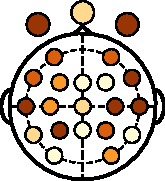
\includegraphics[width=0.17\textwidth]{./img_art_dfa/cabeza_new_VCR_30.pdf} &
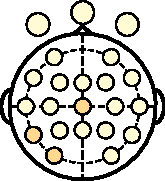
\includegraphics[width=0.17\textwidth]{./img_art_dfa/cabeza_new_MJH_30.pdf} &
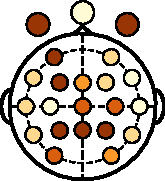
\includegraphics[width=0.17\textwidth]{./img_art_dfa/cabeza_new_JAE_30.pdf} &
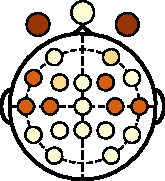
\includegraphics[width=0.17\textwidth]{./img_art_dfa/cabeza_new_GHA_30.pdf} &
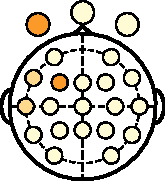
\includegraphics[width=0.17\textwidth]{./img_art_dfa/cabeza_new_MFGR_30.pdf} \\
\midrule
CLO & RLO & RRU & JGZ & AEFP \\
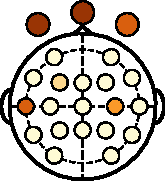
\includegraphics[width=0.17\textwidth]{./img_art_dfa/cabeza_new_CLO_30.pdf} &
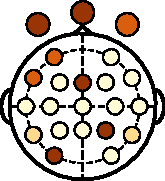
\includegraphics[width=0.17\textwidth]{./img_art_dfa/cabeza_new_RLO_30.pdf} &
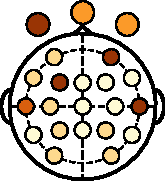
\includegraphics[width=0.17\textwidth]{./img_art_dfa/cabeza_new_RRU_30.pdf} &
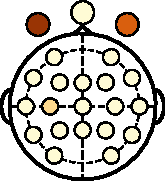
\includegraphics[width=0.17\textwidth]{./img_art_dfa/cabeza_new_JGZ_30.pdf} &
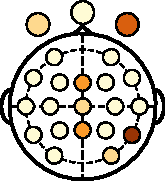
\includegraphics[width=0.17\textwidth]{./img_art_dfa/cabeza_new_AEFP_30.pdf} \\
\end{tabular} \\

\includegraphics[scale=.7]{./img_art_dfa/escala.pdf} \\
\caption{Regiones donde la cantidad de ventanas estacionarias es significativamente diferente 
durante sueño MOR y NMOR, usando ventanas de 30 segundos}
\label{cabeza_new}
\end{figure}

Se repitió la comparación a un nivel grupal, usando la prueba $U$ de  Mann-Whitney.
Se encontraron diferencias significativas para el grupo CTL en los canales P3, P4, PZ, 
ROG y EMG; en el grupo PDC se observaron tales diferencias sólo en P4.
%
Las proporciones muestran tendencias que, quizá, resultaron no ser significativas
por el tamaño pequeño de la muestra: los canales P3 y PZ podrían ser diferentes también para
individuos del grupo PDC, y el canal LOG podría ser diferente durante sueño MOR y NMOR.
%
Así mismo se hipotetiza que para el grupo CTL, en todos los canales, el sueño MOR
es presenta menor cantidad de épocas estacionarias.

Se concluye que
no se puede establecer diferencias entre las medias grupales para esta cantidad (proporción de
épocas estacionarias, medidas en el sentido de PSR), debido a la gran variabilidad entre sujetos.

\begin{figure}
\centering
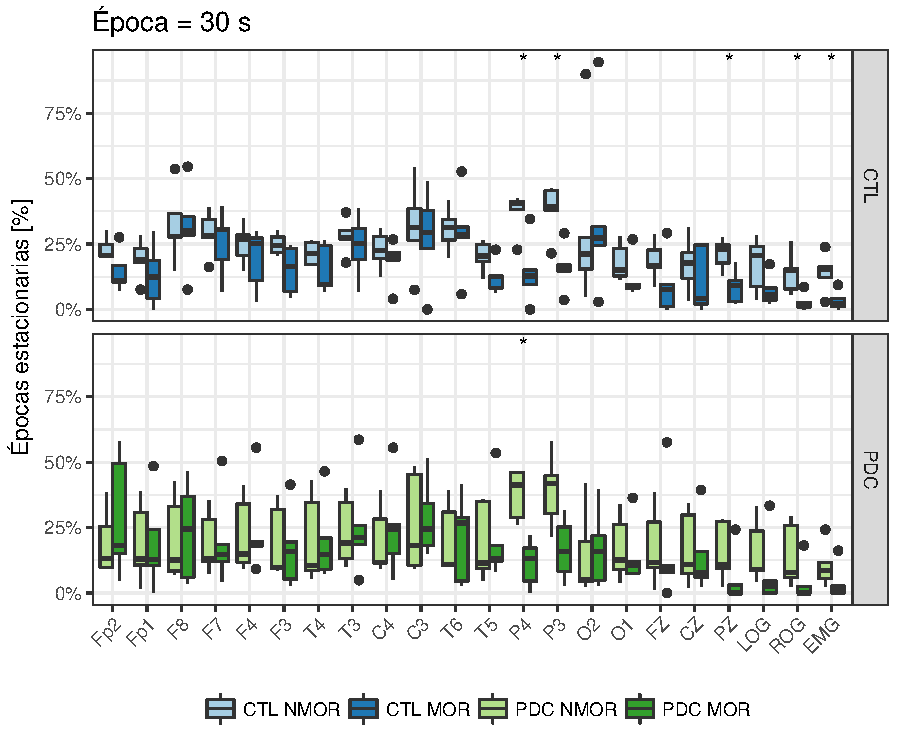
\includegraphics[width=\linewidth]
{./img_art_dfa/Comparacion_gpos_CTL_PDC_v3.pdf}
\caption{Proporciones de épocas estacionarias, durante sueño MOR y NMOR.}
\label{comparacion_verde}
\end{figure}

\begin{figure}
\centering
\includegraphics[width=\linewidth]
{./img_art_dfa/Comparacion_gpos_MOR_NMOR_v3.pdf}
\caption{Proporciones de épocas estacionarias, grupos CTL y PDC.}
\label{comparacion_graf}
\end{figure}

%%%%%%%%%%%%%%%%%%%%%%%%%%%%%%%%%%%%%%%%%%%%%%%%%%%%%%%%%%%%%%%%%%%%%%%%%%%%%%%%%%%%%%%%%%%%%%%%%%%
%%%%%%%%%%%%%%%%%%%%%%%%%%%%%%%%%%%%%%%%%%%%%%%%%%%%%%%%%%%%%%%%%%%%%%%%%%%%%%%%%%%%%%%%%%%%%%%%%%%
%%%%%%%%%%%%%%%%%%%%%%%%%%%%%%%%%%%%%%%%%%%%%%%%%%%%%%%%%%%%%%%%%%%%%%%%%%%%%%%%%%%%%%%%%%%%%%%%%%%

\chapter{Discusión y conclusiones}

Una práctica común en el análisis de señales electrofisiológicas es el suponer que una serie de 
tiempo \textit{suficientemente} corta pueda considerarse estacionaria, cuando menos en el sentido
débil; anteriormente se ha señalado que se trata de un efecto de muestras pequeñas \cite{Melard89},
y paralelamente se han incorporado a los diseños experimentales motivos para mantener este supuesto
\cite{Kaiser00}.

Este trabajo parte de la hipótesis de que adultos mayores con PDC presentan en mayor medida 
estacionariedad débil en sus registros de PSG; al comparar sujetos de los grupo Nn (control) y Mn 
(PDC), no se observaron cambios significativos en la porción de tiempo durante la cual el registro 
de PSG se comporta como débilmente estacionario. 
Esto puede interpretarse como que los cambios en la corteza cerebral durante el deterioro 
cognitivo, no provocan que  la señal se vuelva más \textit{simple} en el sentido de 
\textit{volverse} estacionaria.

Comparando grupalmente la cantidad de épocas estacionarias durante MOR y NMOR, se encontró que en 
el grupo Nn había diferencias significativas en sitios de la región frontal y que no eran presentes
en el grupo Mn; para poder establecer una relación con el PDC haría falta un mayor grupo muestral, 
o bien nuevos registros de PSG para los mismos sujetos, o incluso analizar registros de EEG durante 
otro tipo de actividades y confirmar las diferencias encontradas.

Cabe destacar que la evidencia aportada indica que el PSG es un conjunto de señales que se comportan
como no-estacionarias durante la mayor parte del sueño, lo cual confirma el supuesto usual de que 
las señales de origen biológico son por naturaleza no-estacionarias. 
%\subsection{Efecto del tamaño de las época}

%En el apéndice X se explica que si disminuye el tamaño de época el test de PSR disminuye su 
%potencia, de modo que es más propensa a dar falsos negativos (rechazar la hipótesis de 
%estacionariedad cuando debía aceptarse); entonces, en épocas más pequeñas debería haber más épocas 
%clasificadas como no-estacionarias.
%Sin embargo, al \textit{graficar} la estacionariedad para diferentes tamaños de época (figura
%\ref{comp_VCR}) ocurre que es más frecuente el efecto contrario.
%
%\begin{figure}
%\centering
%\includegraphics[width=\linewidth]{./img_diagramas/epocas_diferentes_v2.pdf}
%\caption{Efecto del tamaño de ventana sobre la clasificación de estacionariedad}
%\label{epocas_diferentes}
%\end{figure}
%
%Se propone que este efecto puede ser explicado si los registros de PSG son \textbf{localmente
%estacionarios}, una propiedad introducida por Dahlhaus \cite{Dahlhaus97} y que consiste en que un
%proceso no-estacionario pueda ser aproximado a trozos \textit{ensamblando} procesos estacionarios
%definidos para intervalos pequeños de tiempo.
%Esta caracterización del EEG ha sido usada anteriormente de manera fructífera pero problemática
%[??].
%
%En el contexto particular del presente trabajo, la presencia de estacionariedad local puede ser
%explicada fisiológicamente por el contenido heterogéneo de ritmos cerebrales de las etapas de 
%sueño; como ejemplo, en la etapa N3 aparecen husos de sueño mezcladas con ritmos Alfa, de modo
%que es posible hallar un fragmento de época en sueño N3 con únicamente un tren de ondas Alfa
%o un tren de husos de sueño.
%Este fenómeno es ilustrado de manera esquemática en la figura \ref{epocas_diferentes}.
%
%
%
%Entonces, se propone que los registros de PSG se comportan como procesos localmente estacionarios; 
%más aún, se propone que esta característica cambia cualitativamente en adultos mayores con PDC,
%para los cuales el \textit{nivel de homogeneidad} del PSG es muy similar durante MOR y NMOR.

%%%%%%%%%%%%%%%%%%%%%%%%%%%%%%%%%%%%%%%%%%%%%%%%%%%%%%%%%%%%%%%%%%%%%%%%%%%%%%%%%%%%%%%%%%%%%%%%%%%
%%%%%%%%%%%%%%%%%%%%%%%%%%%%%%%%%%%%%%%%%%%%%%%%%%%%%%%%%%%%%%%%%%%%%%%%%%%%%%%%%%%%%%%%%%%%%%%%%%%

\section{Conclusiones}

Se concluye que
es posible la ocurrencia de fragmentos arbitrariamente cortos de registros de PSG que no 
son débilmente estacionarios. Paralelamente, la presencia de estos fragmentos se ve influida por el
estado de actividad del cerebro.
%
Como consecuencia directa de este fenómeno, es posible limitar los efectos \textit{distorsivos} de 
la no-estacionariedad, para lo cual basta un diseño experimental que distinga adecuadamente el
estado de actividad a estudiar. 

En otro ámbito, es en principio posible usar la
proporción de estacionariedad (\textit{densidad} de ventanas estacionarias en el sentido de
PSR) en el EEG para caracterizar estados de actividad cerebral. Para ello, falta 
investigar las características particulares de la etapa que se busca identificar, así como otras
etapas cercanas en el tiempo.

%%%%%%%%%%%%%%%%%%%%%%%%%%%%%%%%%%%%%%%%%%%%%%%%%%%%%%%%%%%%%%%%%%%%%%%%%%%%%%%%%%%%%%%%%%%%%%%%%%%
%%%%%%%%%%%%%%%%%%%%%%%%%%%%%%%%%%%%%%%%%%%%%%%%%%%%%%%%%%%%%%%%%%%%%%%%%%%%%%%%%%%%%%%%%%%%%%%%%%%

\section{Trabajo a futuro}

Una vez que se ha identificado un marcador para el PDC usando un grupo de laboratorio,
conviene automatizar los análisis para su uso clínico sobre un público más general.
%
Un uso más amplio de la técnica asegura una mayor población para poder estudiar la 
efectividad y sensibilidad de la prueba
Y más que eso, se espera que puedan ser sinceramente beneficiosos para los pacientes. Siguiendo el
protocolo usual, los marcadores presentados no serán usados como único recurso para generar
un diagnóstico clínico, sino como un apoyo a las herramientas existentes.

El uso de marcadores basados en registros de PSG --basados en el EEG en general-- aporta una
base fisiológica al diagnóstico de deterioro cognitivo, misma que no es posible usando
únicamente pruebas neuropsicológicas.
%
Conviene destacar que, de entre las herramientas para el registro fisiológico del sistema nervioso
central, las técnicas electrofisiológicas son las más económicas y menos invasivas;
generar marcadores basados en ellas facilita su uso por el público general como herramienta 
diagnóstica, sobre todo en ausencia de síntomas.

%%%%%%%%%%%%%%%%%%%%%%%%%%%%%%%%%%%%%%%%%%%%%%%%%%%%%%%%%%%%%%%%%%%%%%%%%%%%%%%%%%%%%%%%%%%%%%%%%%%
%%%%%%%%%%%%%%%%%%%%%%%%%%%%%%%%%%%%%%%%%%%%%%%%%%%%%%%%%%%%%%%%%%%%%%%%%%%%%%%%%%%%%%%%%%%%%%%%%%%
%%%%%%%%%%%%%%%%%%%%%%%%%%%%%%%%%%%%%%%%%%%%%%%%%%%%%%%%%%%%%%%%%%%%%%%%%%%%%%%%%%%%%%%%%%%%%%%%%%%


\appendix

%%%%%%%%%%%%%%%%%%%%%%%%%%%%%%%%%%%%%%%%%%%%%%%%%%%%%%%%%%%%%%%%%%%%%%%%%%%%%%%%%%%%%%%%%%%%%%%%%%%
%%%%%%%%%%%%%%%%%%%%%%%%%%%%%%%%%%%%%%%%%%%%%%%%%%%%%%%%%%%%%%%%%%%%%%%%%%%%%%%%%%%%%%%%%%%%%%%%%%%
%%%%%%%%%%%%%%%%%%%%%%%%%%%%%%%%%%%%%%%%%%%%%%%%%%%%%%%%%%%%%%%%%%%%%%%%%%%%%%%%%%%%%%%%%%%%%%%%%%%
%%%%%%%%%%%%%%%%%%%%%%%%%%%%%%%%%%%%%%%%%%%%%%%%%%%%%%%%%%%%%%%%%%%%%%%%%%%%%%%%%%%%%%%%%%%%%%%%%%%

\chapter{Compilados gráficos}

En este apéndice se muestran los compilados gráficos mencionados en la parte de resultados,
y que representan la
distribución temporal y pseudo-espacial de las ocurrencia de épocas PSG dentro de los registros 
para cada paciente. 

Primeramente se presentan los compilados gráficos en los que se ha destacado el sueño MOR;
posteriormente se presentan los mismos gráficos resaltando los patrones visuales
propuestos, que parecen estar relacionados con la aparición de sueño MOR.


%% parche de relleno
%\begin{figure}
%\centering
%\includegraphics[width=.9\linewidth]{./img_resultados/cabeza_VCR.pdf}
%%\caption{Porcentajes de épocas estacionarias, VCR (VCNNS1)}
%\end{figure}

\begin{figure}
\centering
{\small
\begin{tabular}{lccccc}
\toprule
{\small Tamaño de} & \multicolumn{5}{c}{Grupo CTL} \\
    \cmidrule{2-6}
{\small ventana [s]}    & VCR & MJH & JAE & GHA & MFGR \\
\midrule
$30 \times 2^1$ &
\includegraphics[width=0.13\textwidth]{./img_art_dfa/cabeza_new_VCR_60.pdf} &
\includegraphics[width=0.13\textwidth]{./img_art_dfa/cabeza_new_MJH_60.pdf} &
\includegraphics[width=0.13\textwidth]{./img_art_dfa/cabeza_new_JAE_60.pdf} &
\includegraphics[width=0.13\textwidth]{./img_art_dfa/cabeza_new_GHA_60.pdf} &
\includegraphics[width=0.13\textwidth]{./img_art_dfa/cabeza_new_MFGR_60.pdf} \\
\midrule
$30 \times 2^0$ &
\includegraphics[width=0.13\textwidth]{./img_art_dfa/cabeza_new_VCR_30.pdf} &
\includegraphics[width=0.13\textwidth]{./img_art_dfa/cabeza_new_MJH_30.pdf} &
\includegraphics[width=0.13\textwidth]{./img_art_dfa/cabeza_new_JAE_30.pdf} &
\includegraphics[width=0.13\textwidth]{./img_art_dfa/cabeza_new_GHA_30.pdf} &
\includegraphics[width=0.13\textwidth]{./img_art_dfa/cabeza_new_MFGR_30.pdf} \\
\midrule
$30 \times 2^{-1}$ &
\includegraphics[width=0.13\textwidth]{./img_art_dfa/cabeza_new_VCR_15.pdf} &
\includegraphics[width=0.13\textwidth]{./img_art_dfa/cabeza_new_MJH_15.pdf} &
\includegraphics[width=0.13\textwidth]{./img_art_dfa/cabeza_new_JAE_15.pdf} &
\includegraphics[width=0.13\textwidth]{./img_art_dfa/cabeza_new_GHA_15.pdf} &
\includegraphics[width=0.13\textwidth]{./img_art_dfa/cabeza_new_MFGR_15.pdf} \\
\bottomrule
\end{tabular}\\
\includegraphics[scale=.7]{./img_art_dfa/escala.pdf} \\
}
\end{figure}

\begin{figure}
\centering
{\small
\begin{tabular}{lccccc}
\toprule
{ Tamaño de} & \multicolumn{5}{c}{Grupo PDC} \\
    \cmidrule{2-6}
{ ventana [s]}    & CLO & RLO & RRU & JGZ & AEFP \\
\midrule
$30 \times 2^1$ &
\includegraphics[width=0.13\textwidth]{./img_art_dfa/cabeza_new_CLO_60.pdf} &
\includegraphics[width=0.13\textwidth]{./img_art_dfa/cabeza_new_RLO_60.pdf} &
\includegraphics[width=0.13\textwidth]{./img_art_dfa/cabeza_new_RRU_60.pdf} &
\includegraphics[width=0.13\textwidth]{./img_art_dfa/cabeza_new_JGZ_60.pdf} &
\includegraphics[width=0.13\textwidth]{./img_art_dfa/cabeza_new_AEFP_60.pdf} \\
\midrule
$30 \times 2^0$ &
\includegraphics[width=0.13\textwidth]{./img_art_dfa/cabeza_new_CLO_30.pdf} &
\includegraphics[width=0.13\textwidth]{./img_art_dfa/cabeza_new_RLO_30.pdf} &
\includegraphics[width=0.13\textwidth]{./img_art_dfa/cabeza_new_RRU_30.pdf} &
\includegraphics[width=0.13\textwidth]{./img_art_dfa/cabeza_new_JGZ_30.pdf} &
\includegraphics[width=0.13\textwidth]{./img_art_dfa/cabeza_new_AEFP_30.pdf} \\
\midrule
$30 \times 2^{-1}$ &
\includegraphics[width=0.13\textwidth]{./img_art_dfa/cabeza_new_CLO_15.pdf} &
\includegraphics[width=0.13\textwidth]{./img_art_dfa/cabeza_new_RLO_15.pdf} &
\includegraphics[width=0.13\textwidth]{./img_art_dfa/cabeza_new_RRU_15.pdf} &
\includegraphics[width=0.13\textwidth]{./img_art_dfa/cabeza_new_JGZ_15.pdf} &
\includegraphics[width=0.13\textwidth]{./img_art_dfa/cabeza_new_AEFP_15.pdf} \\
\bottomrule
\end{tabular} \\
\includegraphics[scale=.7]{./img_art_dfa/escala.pdf} \\
}
\caption{Regiones donde la cantidad  de ventanas estacionarias es significativamente diferente
durante MOR y NMOR. Diferentes tamaños de ventana}
\end{figure}

%%%%%%%%%%%%%%%%%%%%%%%%%%%%%%%%%%%%%%%%%%%%%%%%%%%%%%%%%%%%%%%%%%%%%%%%%%%%%%%%%%%%%%%%%%%%%%%%%%%
%%%%%%%%%%%%%%%%%%%%%%%%%%%%%%%%%%%%%%%%%%%%%%%%%%%%%%%%%%%%%%%%%%%%%%%%%%%%%%%%%%%%%%%%%%%%%%%%%%%

\begin{figure}
\begin{subfigure}{\textwidth}
\centering
\includegraphics[width=0.9\linewidth]
{./img_ejemplos/VCNNS1_comp_est_.png} 
\caption{Épocas estacionarias usando diferentes tamaños de ventana}
\end{subfigure}
\end{figure}

\begin{figure}
\ContinuedFloat
\begin{subfigure}{\linewidth}
\centering
\includegraphics[width=0.9\linewidth]
{./enlentecimiento/VCNNS1_espectral_total.png} 
\caption{Espectro de potencias de banda ancha}
\end{subfigure}
\end{figure}

\begin{figure}
\ContinuedFloat
\begin{subfigure}{\linewidth}
\centering
\includegraphics[width=0.9\linewidth]
{./img_resultados/VCNNS1_combinado_.png} 
\caption{Espectro de potencias y análisis de estacionariedad para los canales LOG, ROG y EMG}
\end{subfigure}
\end{figure}

\begin{figure}
\ContinuedFloat
\begin{subfigure}{\linewidth}
\centering
\includegraphics[width=.9\linewidth]{./img_resultados/cabeza_VCR.pdf}
%\caption{Porcentajes de épocas estacionarias, VCR (VCNNS1)}
\caption{Resumen de épocas estacionarias según tamaño de ventana}
\end{subfigure}
\caption{Gráficos individuales para el sujeto VCR}
\end{figure}

%%%%%%%%%%%%%%%%%%%%%%%%%%%%%%%%%%%%%%%%%%%%%%%%%

%\begin{figure}
%\centering
%\includegraphics[width=0.9\linewidth]
%{./img_ejemplos/MJNNVIGILOS_comp_est_.png} 
%\end{figure}
%
%\begin{figure}
%\centering
%\includegraphics[width=0.9\linewidth]
%{./enlentecimiento/MJNNVIGILOS_espectral_total.png} 
%\end{figure}
%
%\begin{figure}
%\centering
%\includegraphics[width=0.9\linewidth]
%{./img_resultados/MJNNVIGILOS_combinado_.png} 
%\end{figure}
%
%\begin{figure}
%\centering
%\includegraphics[width=.9\linewidth]{./img_resultados/cabeza_MJH.pdf}
%%\caption{Porcentajes de épocas estacionarias, MJH (MJNNVIGILOS)}
%\end{figure}
%
%%%%%%%%%%%%%%%%%%%%%%%%%%%%%%%%%%%%%%%%%%%%%%%%%%
%
%\begin{figure}
%\centering
%\includegraphics[width=0.9\linewidth]
%{./img_ejemplos/JANASUE_comp_est_.png} 
%\end{figure}
%\begin{figure}
%\centering
%\includegraphics[width=0.9\linewidth]
%{./enlentecimiento/JANASUE_espectral_total.png} 
%\end{figure}
%\begin{figure}
%\centering
%\includegraphics[width=0.9\linewidth]
%{./img_resultados/JANASUE_combinado_.png} 
%\end{figure}
%
%\begin{figure}
%\centering
%\includegraphics[width=.9\linewidth]{./img_resultados/cabeza_JAE.pdf}
%%\caption{Porcentajes de épocas estacionarias, JAE (JANASUE)}
%\end{figure}
%
%%%%%%%%%%%%%%%%%%%%%%%%%%%%%%%%%%%%%%%%%%%%%%%%%%
%
%\begin{figure}
%\centering
%\includegraphics[width=0.9\linewidth]
%{./img_ejemplos/GH24031950SUENO_comp_est_.png} 
%\end{figure}
%\begin{figure}
%\centering
%\includegraphics[width=0.9\linewidth]
%{./enlentecimiento/GH24031950SUENO_espectral_total.png} 
%\end{figure}
%\begin{figure}
%\centering
%\includegraphics[width=0.9\linewidth]
%{./img_resultados/GH24031950SUENO_combinado_.png} 
%\end{figure}
%
%\begin{figure}
%\centering
%\includegraphics[width=.9\linewidth]{./img_resultados/cabeza_GHA.pdf}
%%\caption{Porcentajes de épocas estacionarias, GHA (GH24031950SUEÑO)}
%\end{figure}
%
%%%%%%%%%%%%%%%%%%%%%%%%%%%%%%%%%%%%%%%%%%%%%%%%%%
%
%\begin{figure}
%\centering
%\includegraphics[width=0.9\linewidth]
%{./img_ejemplos/GURM251148SUE_comp_est_.png} 
%\end{figure}
%\begin{figure}
%\centering
%\includegraphics[width=0.9\linewidth]
%{./enlentecimiento/GURM251148SUE_espectral_total.png} 
%\end{figure}
%\begin{figure}
%\centering
%\includegraphics[width=0.9\linewidth]
%{./img_resultados/GURM251148SUE_combinado_.png} 
%\end{figure}
%
%\begin{figure}
%\centering
%\includegraphics[width=.9\linewidth]{./img_resultados/cabeza_MFGR.pdf}
%%\caption{Porcentajes de épocas estacionarias MFGR (GURM251148SUE)}
%\end{figure}
%
%%%%%%%%%%%%%%%%%%%%%%%%%%%%%%%%%%%%%%
%%%%%%%%%%%%%%%%%%%%%%%%%%%%%%%%%%%%%%
%%%%%%%%%%%%%%%%%%%%%%%%%%%%%%%%%%%%%%
%
%\begin{figure}
%\centering
%\includegraphics[width=0.9\linewidth]
%{./img_ejemplos/CLMN10SUE_comp_est_.png} 
%\end{figure}
%
%\begin{figure}
%\centering
%\includegraphics[width=0.9\linewidth]
%{./enlentecimiento/CLMN10SUE_espectral_total.png} 
%\end{figure}
%
%\begin{figure}
%\centering
%\includegraphics[width=0.9\linewidth]
%{./img_resultados/CLMN10SUE_combinado_.png} 
%\end{figure}
%
%\begin{figure}
%\centering
%\includegraphics[width=.9\linewidth]{./img_resultados/cabeza_CLO.pdf}
%%\caption{Porcentajes de épocas estacionarias, CLO (CLMN10SUE)}
%\end{figure}
%
%%%%%%%%%%%%%%%%%%%%%%%%%%%%%%%%%%%%%%
%
%\begin{figure}
%\centering
%\includegraphics[width=0.9\linewidth]
%{./img_ejemplos/RLMN10SUE_comp_est_.png} 
%\end{figure}
%\begin{figure}
%\centering
%\includegraphics[width=0.9\linewidth]
%{./enlentecimiento/RLMN10SUE_espectral_total.png}
%\end{figure}
%\begin{figure}
%\centering
%\includegraphics[width=0.9\linewidth]
%{./img_ejemplos/RLMN10SUE_comp_est_.png} 
%\end{figure}
%
%\begin{figure}
%\centering
%\includegraphics[width=.9\linewidth]{./img_resultados/cabeza_RLO.pdf}
%%\caption{Porcentajes de épocas estacionarias, RLO (RLMN10SUE)}
%\end{figure}
%
%%%%%%%%%%%%%%%%%%%%%%%%%%%%%%%%%%%%%%
%
%\begin{figure}
%\centering
%\includegraphics[width=0.9\linewidth]
%{./img_ejemplos/RRMNS_comp_est_.png} 
%\end{figure}
%
%\begin{figure}
%\centering
%\includegraphics[width=0.9\linewidth]
%{./enlentecimiento/RRMNS_espectral_total.png}
%\end{figure}
%
%\begin{figure}
%\centering
%\includegraphics[width=0.9\linewidth]
%{./img_resultados/RRMNS_combinado_.png} 
%\end{figure}
%
%\begin{figure}
%\centering
%\includegraphics[width=.9\linewidth]{./img_resultados/cabeza_RRU.pdf}
%%\caption{Porcentajes de épocas estacionarias, RRU (RRMNS)}
%\end{figure}
%
%%%%%%%%%%%%%%%%%%%%%%%%%%%%%%%%%%%%%%
%
%\begin{figure}
%\centering
%\includegraphics[width=0.9\linewidth]
%{./img_ejemplos/JGMN6SUE_comp_est_.png} 
%\end{figure}
%
%\begin{figure}
%\centering
%\includegraphics[width=0.9\linewidth]
%{./enlentecimiento/JGMN6SUE_espectral_total.png} 
%\end{figure}
%
%\begin{figure}
%\centering
%\includegraphics[width=0.9\linewidth]
%{./img_resultados/JGMN6SUE_combinado_.png} 
%\end{figure}
%
%\begin{figure}
%\centering
%\includegraphics[width=.9\linewidth]{./img_resultados/cabeza_JGZ.pdf}
%%\caption{Porcentajes de épocas estacionarias, JGZ (JGMN6SUE)}
%\end{figure}
%
%%%%%%%%%%%%%%%%%%%%%%%%%%%%%%%%%%%%%%
%%%%%%%%%%%%%%%%%%%%%%%%%%%%%%%%%%%%%%
%%%%%%%%%%%%%%%%%%%%%%%%%%%%%%%%%%%%%%
%
%%\begin{figure}
%%\centering
%%\includegraphics[width=0.9\linewidth]
%%{./img_ejemplos/FGHSUE_comp_est_.png} 
%%\end{figure}
%%\begin{figure}
%%\centering
%%\includegraphics[width=0.9\linewidth]
%%{./img_resultados/FGHSUE_espectral_total.png} 
%%\end{figure}
%%\begin{figure}
%%\centering
%%\includegraphics[width=0.9\linewidth]
%%{./img_resultados/FGHSUE_combinado_.png} 
%%\end{figure}
%%
%%\begin{figure}
%%\centering
%%\includegraphics[width=.9\linewidth]{./img_resultados/cabeza_FGH.pdf}
%%%\caption{Porcentajes de épocas estacionarias, FGH (FGHSUE)}
%%\end{figure}
%
%%%%%%%%%%%%%%%%%%%%%%%%%%%%%%%%%%%%%%
%
%%\begin{figure}
%%\centering
%%\includegraphics[width=0.9\linewidth]
%%{./img_ejemplos/MGNA5SUE_comp_est_.png} 
%%\end{figure}
%%\begin{figure}
%%\centering
%%\includegraphics[width=0.9\linewidth]
%%{./img_resultados/MGNA5SUE_espectral_total.png} 
%%\end{figure}
%%\begin{figure}
%%\centering
%%\includegraphics[width=0.9\linewidth]
%%{./img_resultados/MGNA5SUE_combinado_.png} 
%%\end{figure}
%%
%%\begin{figure}
%%\centering
%%\includegraphics[width=.9\linewidth]{./img_resultados/cabeza_MGG.pdf}
%%%\caption{Porcentajes de épocas estacionarias, MGG (MGNA5SUE)}
%%\end{figure}
%
%%%%%%%%%%%%%%%%%%%%%%%%%%%%%%%%%%%%%%
%
%%\begin{figure}
%%\centering
%%\includegraphics[width=0.9\linewidth]
%%{./img_ejemplos/EMNNS_comp_est_.png} 
%%\end{figure}
%%\begin{figure}
%%\centering
%%\includegraphics[width=0.9\linewidth]
%%{./img_ejemplos/EMNNS_comp_est_.png} 
%%\end{figure}
%%\begin{figure}
%%\centering
%%\includegraphics[width=0.9\linewidth]
%%{./img_ejemplos/EMNNS_comp_est_.png} 
%%\end{figure}
%%
%%\begin{figure}
%%\centering
%%\includegraphics[width=.9\linewidth]{./img_resultados/cabeza_EMT.pdf}
%%%\caption{Porcentajes de épocas estacionarias EMT (EMNNS)}
%%\end{figure}
%
%%%%%%%%%%%%%%%%%%%%%%%%%%%%%%%%%%%%%%
%
%%\begin{figure}
%%\bordes{1.5}
%%\begin{tabular}{l}
%%\Large{{Patrones visuales}}\\
%%\begin{tabular}{c}
%%\includegraphics[width=0.45\textwidth]
%%{./img_ejemplos/zoom_VCR.pdf}
%%\includegraphics[width=0.45\textwidth]
%%{./img_ejemplos/zoom_MJH.pdf}
%%\\
%%\includegraphics[width=0.45\textwidth]
%%{./img_ejemplos/zoom_JAE.pdf}
%%\includegraphics[width=0.45\textwidth]
%%{./img_ejemplos/zoom_GHA.pdf}
%%\\
%%\includegraphics[width=0.45\textwidth]
%%{./img_ejemplos/zoom_MFGR.pdf}
%%\end{tabular}
%%\end{tabular}
%%\end{figure}
%
%%%%%%%%%%%%%%%%%%%%%%%%%%%%%%%%%%%%%%%%%%%%%%%%%%%%%%%%%%%%%%%%%%%%%%%%%%%%%%%%%%%%%%%%%%%%%%%%%%%%
%%%%%%%%%%%%%%%%%%%%%%%%%%%%%%%%%%%%%%%%%%%%%%%%%%%%%%%%%%%%%%%%%%%%%%%%%%%%%%%%%%%%%%%%%%%%%%%%%%%%
%%%%%%%%%%%%%%%%%%%%%%%%%%%%%%%%%%%%%%%%%%%%%%%%%%%%%%%%%%%%%%%%%%%%%%%%%%%%%%%%%%%%%%%%%%%%%%%%%%%%
%%%%%%%%%%%%%%%%%%%%%%%%%%%%%%%%%%%%%%%%%%%%%%%%%%%%%%%%%%%%%%%%%%%%%%%%%%%%%%%%%%%%%%%%%%%%%%%%%%%%


%%%%%%%%%%%%%%%%%%%%%%%%%%%%%%%%%%%%%%%%%%%%%%%%%%%%%%%%%%%%%%%%%%%%%%%%%%%%%%%%%%%%%%%%%%%%%%%%%%%
%%%%%%%%%%%%%%%%%%%%%%%%%%%%%%%%%%%%%%%%%%%%%%%%%%%%%%%%%%%%%%%%%%%%%%%%%%%%%%%%%%%%%%%%%%%%%%%%%%%

\chapter*{Glosario}
\addcontentsline{toc}{chapter}{Glosario}

{
\setlength{\leftskip}{2em}
\setlength{\parindent}{-2em}

\textbf{AABFM:} Actividad de Amplitud Baja y Frecuencias Mixtas \\
Actividad de amplitud relativamente baja ($<10$ \mv), visualmente desorganizada.
No tiene una forma sinusoidal clara.

\textbf{AASM:} American Academy of Sleep Medicine \\
Sociedad estadounidense dedicada al estudio de la \textit{Medicina del sueño} (relativo al 
diagnóstico y tratamiento de trastornos del sueño).
En dicha área, los estándares establecidos por esta organización se encuentran ampliamente 
difundidos.

\textbf{DCL:} Deterioro Cognitivo Leve \\
Conjunto de deficiencias cognitivas \textit{objetivas}, respecto a un estado anterior, que no cumplen los criterios para ser clasificadas como demencia. 
Para ello se entiende que una deficiencia es objetiva si puede confirmarse usando pruebas neuropsicológicas, en contraposición al reporte subjetiva por parte del individuo.

\textbf{EEG:}  Electroencefalografía \\
Lectura de la actividad eléctrica en la corteza cerebral, la cual se origina por la actividad postsináptica de las neuronas en dicha región. 
En el presente trabajo, el término EEG se limita a registros obtenidos mediante electrodos colocados en el cuero cabelludo del individuo, siendo que otros autores también engloban registros obtenidos con microelectrodos insertos en el cerebro por ejemplo.

\textbf{EMG:}  Electromiografía \\
Lectura de la actividad eléctrica en las fibras musculares, la cual se origina por el reclutamiento y activación de fibras musculares por parte del sistema nervioso.
En el presente trabajo, se limita el uso del EMG para distinguir la mayor o menor presencia de \textit{tono muscular}, fenómeno característico de fibras musculares en actividad latente.

\textbf{EOG:}  Electrooculografía \\

\textbf{MOR:} [Sueño de] Movimientos Oculares Rápidos \\
%Etapa del sueño profundo caracterizada por la presencia de movimientos oculares rápidos, disminución del tono muscular, y actividad eléctrica cerebral de baja intensidad y frecuencias mixtas.
Etapa de sueño nombrada con base la presencia típica de movimientos oculares rápidos. También se le conoce como \textit{sueño paradójico} debido a que la actividad cerebral es similar a la vigilia pese a ser la etapa más profunda del sueño. Según los estándares de la AASM en 2007 también se le conoce como \textit{fase R}.

\textbf{NMOR:} [Sueño] No-MOR \\
Contempla el sueño fuera de la etapa MOR, presentando características radicalmente diferentes.
%También se conoce como \textit{sueño de ondas lentas} por las ondas
Pese a su definición negativa, se divide en sub-etapas con características distintivas claras.
Según los estándares de la AASM en 2007 también se le conoce como \textit{fase N}.

\textbf{PSG:}  Polisomnografía \\
Registro conjunto durante el sueño de varias señales electrofisiológicas u otros indicadores fisiológicos.

\textbf{PDC:}  Posible Deterioro Cognitivo [Leve] \\
Diagnóstico positivo para deterioro cognitivo usando únicamente los resultados de pruebas neuropsicológicas, y en particular las usadas en el presente trabajo.
Debido a los estándares cautelosos de la psicología clínica, para otorgar el diagnóstico de \textit{deterioro cognitivo leve} no puede otorgarse deben tomarse en cuenta varios estudios complementarios, como imagenología del cerebro por ejemplo.

}

\section*{Catálogo de funciones comunes}
{
\setlength{\leftskip}{2em}
\setlength{\parindent}{-2em}

\textbf{Delta de Kroneker ($\delta$)} \\
Usada para facilitar la descripción de productos ortogonales.
\begin{equation*}
\delta(i,j) = \begin{cases}
1 &, i = j \\
0 &, i \neq j
\end{cases}
\end{equation*}

\textbf{H de Heavyside ($H$)} \\
Usada para facilitar la descripción de \textit{ondas cuadradas}.
\begin{equation*}
H(x) = \begin{cases}
1 &, x>0 \\
0 &, x=0 \\
-1 &, x<0
\end{cases}
\end{equation*}

\textbf{O mayúscula de Landau ($\mathcal{O}$)} \\
Sean $f, g : \R \rightarrow \R$ dos funciones y $x_0 \in \R \cup \{ -\infty, \infty\}$ arbitrario. Se dice que $f$ es \textit{de orden $g$ alrededor de $x_0$} si existe $C \in \R$ tal que
\begin{equation*}
\lim_{x \rightarrow x_0} \frac{f(x)}{g(x)} = C
\end{equation*} 
en cuyo caso se dice $f = \orden{g}$
}

%%%%%%%%%%%%%%%%%%%%%%%%%%%%%%%%%%%%%%%%%%%%%%%%%%%%%%%%%%%%%%%%%%%%%%%%%%%%%%%%%%%%%%%%%%%%%%%%%%%
%%%%%%%%%%%%%%%%%%%%%%%%%%%%%%%%%%%%%%%%%%%%%%%%%%%%%%%%%%%%%%%%%%%%%%%%%%%%%%%%%%%%%%%%%%%%%%%%%%%

\pagestyle{plain}

\bibliographystyle{bababbrv-lf}
\bibliography{referencias_estacionariedad,referencias_fisiologia,referencias_otros,referencias_mixto}%{}

%%%%%%%%%%%%%%%%%%%%%%%%%%%%%%%%%%%%%%%%%%%%%%%%%%%%%%%%%%%%%%%%%%%%%%%%%%%%%%%%%%%%%%%%%%%%%%%%%%%
%%%%%%%%%%%%%%%%%%%%%%%%%%%%%%%%%%%%%%%%%%%%%%%%%%%%%%%%%%%%%%%%%%%%%%%%%%%%%%%%%%%%%%%%%%%%%%%%%%%

\end{document}

%%%%%%%%%%%%%%%%%%%%%%%%%%%%%%%%%%%%%%%%%%%%%%%%%%%%%%%%%%%%%%%%%%%%%%%%%%%%%%%%%%%%%%%%%%%%%%%%%%%
%%%%%%%%%%%%%%%%%%%%%%%%%%%%%%%%%%%%%%%%%%%%%%%%%%%%%%%%%%%%%%%%%%%%%%%%%%%%%%%%%%%%%%%%%%%%%%%%%%%
%%%%%%%%%%%%%%%%%%%%%%%%%%%%%%%%%%%%%%%%%%%%%%%%%%%%%%%%%%%%%%%%%%%%%%%%%%%%%%%%%%%%%%%%%%%%%%%%%%%
%%%%%%%%%%%%%%%%%%%%%%%%%%%%%%%%%%%%%%%%%%%%%%%%%%%%%%%%%%%%%%%%%%%%%%%%%%%%%%%%%%%%%%%%%%%%%%%%%%%